\documentclass[twoside]{book}

% Packages required by doxygen
\usepackage{fixltx2e}
\usepackage{calc}
\usepackage{doxygen}
\usepackage[export]{adjustbox} % also loads graphicx
\usepackage{graphicx}
\usepackage[utf8]{inputenc}
\usepackage{makeidx}
\usepackage{multicol}
\usepackage{multirow}
\PassOptionsToPackage{warn}{textcomp}
\usepackage{textcomp}
\usepackage[nointegrals]{wasysym}
\usepackage[table]{xcolor}

% Font selection
\usepackage[T1]{fontenc}
\usepackage[scaled=.90]{helvet}
\usepackage{courier}
\usepackage{amssymb}
\usepackage{sectsty}
\renewcommand{\familydefault}{\sfdefault}
\allsectionsfont{%
  \fontseries{bc}\selectfont%
  \color{darkgray}%
}
\renewcommand{\DoxyLabelFont}{%
  \fontseries{bc}\selectfont%
  \color{darkgray}%
}
\newcommand{\+}{\discretionary{\mbox{\scriptsize$\hookleftarrow$}}{}{}}

% Page & text layout
\usepackage{geometry}
\geometry{%
  a4paper,%
  top=2.5cm,%
  bottom=2.5cm,%
  left=2.5cm,%
  right=2.5cm%
}
\tolerance=750
\hfuzz=15pt
\hbadness=750
\setlength{\emergencystretch}{15pt}
\setlength{\parindent}{0cm}
\setlength{\parskip}{3ex plus 2ex minus 2ex}
\makeatletter
\renewcommand{\paragraph}{%
  \@startsection{paragraph}{4}{0ex}{-1.0ex}{1.0ex}{%
    \normalfont\normalsize\bfseries\SS@parafont%
  }%
}
\renewcommand{\subparagraph}{%
  \@startsection{subparagraph}{5}{0ex}{-1.0ex}{1.0ex}{%
    \normalfont\normalsize\bfseries\SS@subparafont%
  }%
}
\makeatother

% Headers & footers
\usepackage{fancyhdr}
\pagestyle{fancyplain}
\fancyhead[LE]{\fancyplain{}{\bfseries\thepage}}
\fancyhead[CE]{\fancyplain{}{}}
\fancyhead[RE]{\fancyplain{}{\bfseries\leftmark}}
\fancyhead[LO]{\fancyplain{}{\bfseries\rightmark}}
\fancyhead[CO]{\fancyplain{}{}}
\fancyhead[RO]{\fancyplain{}{\bfseries\thepage}}
\fancyfoot[LE]{\fancyplain{}{}}
\fancyfoot[CE]{\fancyplain{}{}}
\fancyfoot[RE]{\fancyplain{}{\bfseries\scriptsize Generated by Doxygen }}
\fancyfoot[LO]{\fancyplain{}{\bfseries\scriptsize Generated by Doxygen }}
\fancyfoot[CO]{\fancyplain{}{}}
\fancyfoot[RO]{\fancyplain{}{}}
\renewcommand{\footrulewidth}{0.4pt}
\renewcommand{\chaptermark}[1]{%
  \markboth{#1}{}%
}
\renewcommand{\sectionmark}[1]{%
  \markright{\thesection\ #1}%
}

% Indices & bibliography
\usepackage{natbib}
\usepackage[titles]{tocloft}
\setcounter{tocdepth}{3}
\setcounter{secnumdepth}{5}
\makeindex

% Hyperlinks (required, but should be loaded last)
\usepackage{ifpdf}
\ifpdf
  \usepackage[pdftex,pagebackref=true]{hyperref}
\else
  \usepackage[ps2pdf,pagebackref=true]{hyperref}
\fi
\hypersetup{%
  colorlinks=true,%
  linkcolor=blue,%
  citecolor=blue,%
  unicode%
}

% Custom commands
\newcommand{\clearemptydoublepage}{%
  \newpage{\pagestyle{empty}\cleardoublepage}%
}

\usepackage{caption}
\captionsetup{labelsep=space,justification=centering,font={bf},singlelinecheck=off,skip=4pt,position=top}

%===== C O N T E N T S =====

\begin{document}

% Titlepage & ToC
\hypersetup{pageanchor=false,
             bookmarksnumbered=true,
             pdfencoding=unicode
            }
\pagenumbering{roman}
\begin{titlepage}
\vspace*{7cm}
\begin{center}%
{\Large My Project }\\
\vspace*{1cm}
{\large Generated by Doxygen 1.8.11}\\
\end{center}
\end{titlepage}
\clearemptydoublepage
\tableofcontents
\clearemptydoublepage
\pagenumbering{arabic}
\hypersetup{pageanchor=true}

%--- Begin generated contents ---
\chapter{Namespace Index}
\section{Namespace List}
Here is a list of all namespaces with brief descriptions\+:\begin{DoxyCompactList}
\item\contentsline{section}{\hyperlink{namespace_k}{K} }{\pageref{namespace_k}}{}
\end{DoxyCompactList}

\chapter{Hierarchical Index}
\section{Class Hierarchy}
This inheritance list is sorted roughly, but not completely, alphabetically\+:\begin{DoxyCompactList}
\item \contentsline{section}{FN}{\pageref{class_k_1_1_f_n}}{}
\item \contentsline{section}{Gw}{\pageref{class_k_1_1_gw}}{}
\item \contentsline{section}{Klass}{\pageref{class_k_1_1_klass}}{}
\begin{DoxyCompactList}
\item \contentsline{section}{DB}{\pageref{class_k_1_1_d_b}}{}
\item \contentsline{section}{EV}{\pageref{class_k_1_1_e_v}}{}
\item \contentsline{section}{GW}{\pageref{class_k_1_1_g_w}}{}
\item \contentsline{section}{k\+Lass}{\pageref{class_k_1_1k_lass}}{}
\begin{DoxyCompactList}
\item \contentsline{section}{CF}{\pageref{class_k_1_1_c_f}}{}
\end{DoxyCompactList}
\item \contentsline{section}{MG}{\pageref{class_k_1_1_m_g}}{}
\item \contentsline{section}{OG}{\pageref{class_k_1_1_o_g}}{}
\item \contentsline{section}{PG}{\pageref{class_k_1_1_p_g}}{}
\item \contentsline{section}{QE}{\pageref{class_k_1_1_q_e}}{}
\item \contentsline{section}{QP}{\pageref{class_k_1_1_q_p}}{}
\item \contentsline{section}{UI}{\pageref{class_k_1_1_u_i}}{}
\end{DoxyCompactList}
\item \contentsline{section}{m\+Level}{\pageref{struct_k_1_1m_level}}{}
\item \contentsline{section}{m\+Levels}{\pageref{struct_k_1_1m_levels}}{}
\begin{DoxyCompactList}
\item \contentsline{section}{m\+Levels\+Diff}{\pageref{struct_k_1_1m_levels_diff}}{}
\end{DoxyCompactList}
\item \contentsline{section}{m\+Order}{\pageref{struct_k_1_1m_order}}{}
\item \contentsline{section}{m\+Pair}{\pageref{struct_k_1_1m_pair}}{}
\item \contentsline{section}{m\+Position}{\pageref{struct_k_1_1m_position}}{}
\item \contentsline{section}{m\+Profit}{\pageref{struct_k_1_1m_profit}}{}
\item \contentsline{section}{m\+Quote}{\pageref{struct_k_1_1m_quote}}{}
\item \contentsline{section}{m\+Quote\+Status}{\pageref{struct_k_1_1m_quote_status}}{}
\item \contentsline{section}{m\+Quoting\+Params}{\pageref{struct_k_1_1m_quoting_params}}{}
\item \contentsline{section}{m\+Safety}{\pageref{struct_k_1_1m_safety}}{}
\item \contentsline{section}{m\+Trade}{\pageref{struct_k_1_1m_trade}}{}
\item \contentsline{section}{m\+Wallet}{\pageref{struct_k_1_1m_wallet}}{}
\item \contentsline{section}{m\+Wallets}{\pageref{struct_k_1_1m_wallets}}{}
\item \contentsline{section}{SH}{\pageref{class_k_1_1_s_h}}{}
\end{DoxyCompactList}

\chapter{Data Structure Index}
\section{Data Structures}
Here are the data structures with brief descriptions\+:\begin{DoxyCompactList}
\item\contentsline{section}{\hyperlink{class_k_1_1_c_f}{CF} }{\pageref{class_k_1_1_c_f}}{}
\item\contentsline{section}{\hyperlink{class_k_1_1_d_b}{DB} }{\pageref{class_k_1_1_d_b}}{}
\item\contentsline{section}{\hyperlink{class_k_1_1_e_v}{EV} }{\pageref{class_k_1_1_e_v}}{}
\item\contentsline{section}{\hyperlink{class_k_1_1_f_n}{FN} }{\pageref{class_k_1_1_f_n}}{}
\item\contentsline{section}{\hyperlink{class_k_1_1_g_w}{GW} }{\pageref{class_k_1_1_g_w}}{}
\item\contentsline{section}{\hyperlink{class_k_1_1_gw}{Gw} }{\pageref{class_k_1_1_gw}}{}
\item\contentsline{section}{\hyperlink{class_k_1_1_klass}{Klass} }{\pageref{class_k_1_1_klass}}{}
\item\contentsline{section}{\hyperlink{class_k_1_1k_lass}{k\+Lass} }{\pageref{class_k_1_1k_lass}}{}
\item\contentsline{section}{\hyperlink{class_k_1_1_m_g}{MG} }{\pageref{class_k_1_1_m_g}}{}
\item\contentsline{section}{\hyperlink{struct_k_1_1m_level}{m\+Level} }{\pageref{struct_k_1_1m_level}}{}
\item\contentsline{section}{\hyperlink{struct_k_1_1m_levels}{m\+Levels} }{\pageref{struct_k_1_1m_levels}}{}
\item\contentsline{section}{\hyperlink{struct_k_1_1m_levels_diff}{m\+Levels\+Diff} }{\pageref{struct_k_1_1m_levels_diff}}{}
\item\contentsline{section}{\hyperlink{struct_k_1_1m_order}{m\+Order} }{\pageref{struct_k_1_1m_order}}{}
\item\contentsline{section}{\hyperlink{struct_k_1_1m_pair}{m\+Pair} }{\pageref{struct_k_1_1m_pair}}{}
\item\contentsline{section}{\hyperlink{struct_k_1_1m_position}{m\+Position} }{\pageref{struct_k_1_1m_position}}{}
\item\contentsline{section}{\hyperlink{struct_k_1_1m_profit}{m\+Profit} }{\pageref{struct_k_1_1m_profit}}{}
\item\contentsline{section}{\hyperlink{struct_k_1_1m_quote}{m\+Quote} }{\pageref{struct_k_1_1m_quote}}{}
\item\contentsline{section}{\hyperlink{struct_k_1_1m_quote_status}{m\+Quote\+Status} }{\pageref{struct_k_1_1m_quote_status}}{}
\item\contentsline{section}{\hyperlink{struct_k_1_1m_quoting_params}{m\+Quoting\+Params} }{\pageref{struct_k_1_1m_quoting_params}}{}
\item\contentsline{section}{\hyperlink{struct_k_1_1m_safety}{m\+Safety} }{\pageref{struct_k_1_1m_safety}}{}
\item\contentsline{section}{\hyperlink{struct_k_1_1m_trade}{m\+Trade} }{\pageref{struct_k_1_1m_trade}}{}
\item\contentsline{section}{\hyperlink{struct_k_1_1m_wallet}{m\+Wallet} }{\pageref{struct_k_1_1m_wallet}}{}
\item\contentsline{section}{\hyperlink{struct_k_1_1m_wallets}{m\+Wallets} }{\pageref{struct_k_1_1m_wallets}}{}
\item\contentsline{section}{\hyperlink{class_k_1_1_o_g}{OG} }{\pageref{class_k_1_1_o_g}}{}
\item\contentsline{section}{\hyperlink{class_k_1_1_p_g}{PG} }{\pageref{class_k_1_1_p_g}}{}
\item\contentsline{section}{\hyperlink{class_k_1_1_q_e}{QE} }{\pageref{class_k_1_1_q_e}}{}
\item\contentsline{section}{\hyperlink{class_k_1_1_q_p}{QP} }{\pageref{class_k_1_1_q_p}}{}
\item\contentsline{section}{\hyperlink{class_k_1_1_s_h}{SH} }{\pageref{class_k_1_1_s_h}}{}
\item\contentsline{section}{\hyperlink{class_k_1_1_u_i}{UI} }{\pageref{class_k_1_1_u_i}}{}
\end{DoxyCompactList}

\chapter{File Index}
\section{File List}
Here is a list of all files with brief descriptions\+:\begin{DoxyCompactList}
\item\contentsline{section}{\hyperlink{cf_8h}{cf.\+h} }{\pageref{cf_8h}}{}
\item\contentsline{section}{\hyperlink{db_8h}{db.\+h} }{\pageref{db_8h}}{}
\item\contentsline{section}{\hyperlink{ev_8h}{ev.\+h} }{\pageref{ev_8h}}{}
\item\contentsline{section}{\hyperlink{fn_8h}{fn.\+h} }{\pageref{fn_8h}}{}
\item\contentsline{section}{\hyperlink{gw_8h}{gw.\+h} }{\pageref{gw_8h}}{}
\item\contentsline{section}{\hyperlink{_k_8cxx}{K.\+cxx} }{\pageref{_k_8cxx}}{}
\item\contentsline{section}{\hyperlink{km_8h}{km.\+h} }{\pageref{km_8h}}{}
\item\contentsline{section}{\hyperlink{mg_8h}{mg.\+h} }{\pageref{mg_8h}}{}
\item\contentsline{section}{\hyperlink{og_8h}{og.\+h} }{\pageref{og_8h}}{}
\item\contentsline{section}{\hyperlink{pg_8h}{pg.\+h} }{\pageref{pg_8h}}{}
\item\contentsline{section}{\hyperlink{qe_8h}{qe.\+h} }{\pageref{qe_8h}}{}
\item\contentsline{section}{\hyperlink{qp_8h}{qp.\+h} }{\pageref{qp_8h}}{}
\item\contentsline{section}{\hyperlink{sh_8h}{sh.\+h} }{\pageref{sh_8h}}{}
\item\contentsline{section}{\hyperlink{ui_8h}{ui.\+h} }{\pageref{ui_8h}}{}
\end{DoxyCompactList}

\chapter{Namespace Documentation}
\hypertarget{namespace_k}{}\section{K Namespace Reference}
\label{namespace_k}\index{K@{K}}
\subsection*{Data Structures}
\begin{DoxyCompactItemize}
\item 
class \hyperlink{class_k_1_1_c_f}{CF}
\item 
class \hyperlink{class_k_1_1_d_b}{DB}
\item 
class \hyperlink{class_k_1_1_e_v}{EV}
\item 
class \hyperlink{class_k_1_1_f_n}{FN}
\item 
class \hyperlink{class_k_1_1_g_w}{GW}
\item 
class \hyperlink{class_k_1_1_gw}{Gw}
\item 
class \hyperlink{class_k_1_1_klass}{Klass}
\item 
class \hyperlink{class_k_1_1k_lass}{k\+Lass}
\item 
class \hyperlink{class_k_1_1_m_g}{MG}
\item 
struct \hyperlink{struct_k_1_1m_level}{m\+Level}
\item 
struct \hyperlink{struct_k_1_1m_levels}{m\+Levels}
\item 
struct \hyperlink{struct_k_1_1m_levels_diff}{m\+Levels\+Diff}
\item 
struct \hyperlink{struct_k_1_1m_order}{m\+Order}
\item 
struct \hyperlink{struct_k_1_1m_pair}{m\+Pair}
\item 
struct \hyperlink{struct_k_1_1m_position}{m\+Position}
\item 
struct \hyperlink{struct_k_1_1m_profit}{m\+Profit}
\item 
struct \hyperlink{struct_k_1_1m_quote}{m\+Quote}
\item 
struct \hyperlink{struct_k_1_1m_quote_status}{m\+Quote\+Status}
\item 
struct \hyperlink{struct_k_1_1m_quoting_params}{m\+Quoting\+Params}
\item 
struct \hyperlink{struct_k_1_1m_safety}{m\+Safety}
\item 
struct \hyperlink{struct_k_1_1m_trade}{m\+Trade}
\item 
struct \hyperlink{struct_k_1_1m_wallet}{m\+Wallet}
\item 
struct \hyperlink{struct_k_1_1m_wallets}{m\+Wallets}
\item 
class \hyperlink{class_k_1_1_o_g}{OG}
\item 
class \hyperlink{class_k_1_1_p_g}{PG}
\item 
class \hyperlink{class_k_1_1_q_e}{QE}
\item 
class \hyperlink{class_k_1_1_q_p}{QP}
\item 
class \hyperlink{class_k_1_1_s_h}{SH}
\item 
class \hyperlink{class_k_1_1_u_i}{UI}
\end{DoxyCompactItemize}
\subsection*{Enumerations}
\begin{DoxyCompactItemize}
\item 
enum \hyperlink{namespace_k_a7ab53d1849aa2c29d90459c21afa8c17}{m\+Exchange} \+: unsigned int \{ \\*
\hyperlink{namespace_k_a7ab53d1849aa2c29d90459c21afa8c17abbb93ef26e3c101ff11cdd21cab08a94}{Null}, 
\hyperlink{namespace_k_a7ab53d1849aa2c29d90459c21afa8c17ae05277537bf941fa13c912696bf55c2f}{Hit\+Btc}, 
\hyperlink{namespace_k_a7ab53d1849aa2c29d90459c21afa8c17a6af33051ce1839b748ad2f59cb203e0f}{Ok\+Coin}, 
\hyperlink{namespace_k_a7ab53d1849aa2c29d90459c21afa8c17a28d13ddddf18afba2c3727253ba0d42f}{Coinbase}, 
\\*
\hyperlink{namespace_k_a7ab53d1849aa2c29d90459c21afa8c17a4e7d470f48dde438b7e7ee118231262d}{Bitfinex}, 
\hyperlink{namespace_k_a7ab53d1849aa2c29d90459c21afa8c17a049a956dfeb0eb2e19c417a1dde4d680}{Kraken}, 
\hyperlink{namespace_k_a7ab53d1849aa2c29d90459c21afa8c17a1299d85e255e3e8967042390b25dffd3}{Ok\+Ex}, 
\hyperlink{namespace_k_a7ab53d1849aa2c29d90459c21afa8c17ac17831afdb4609a6f28e6f361c67b55f}{Bitfinex\+Margin}, 
\\*
\hyperlink{namespace_k_a7ab53d1849aa2c29d90459c21afa8c17a58fbcde0e62c0d61a359ac2cab9418c6}{Korbit}, 
\hyperlink{namespace_k_a7ab53d1849aa2c29d90459c21afa8c17a90239374e2208c9b3ad9d6ead6d875b8}{Poloniex}
 \}
\item 
enum \hyperlink{namespace_k_a3da250819294c55d5728586148bfa19e}{m\+Connectivity} \+: unsigned int \{ \hyperlink{namespace_k_a3da250819294c55d5728586148bfa19eaef70e46fd3bbc21e3e1f0b6815e750c0}{Disconnected}, 
\hyperlink{namespace_k_a3da250819294c55d5728586148bfa19ea2ec0d16e4ca169baedb9b2d50ec5c6d7}{Connected}
 \}
\item 
enum \hyperlink{namespace_k_a9ca92b450f3b1738c485770d136ac9e0}{m\+Status} \+: unsigned int \{ \hyperlink{namespace_k_a9ca92b450f3b1738c485770d136ac9e0a03c2e7e41ffc181a4e84080b4710e81e}{New}, 
\hyperlink{namespace_k_a9ca92b450f3b1738c485770d136ac9e0a829eadc8e29caab50cc26bc6a451a1f1}{Working}, 
\hyperlink{namespace_k_a9ca92b450f3b1738c485770d136ac9e0aae94f80b3ce82062a5dd7815daa04f9d}{Complete}, 
\hyperlink{namespace_k_a9ca92b450f3b1738c485770d136ac9e0aa149e85a44aeec9140e92733d9ed694e}{Cancelled}
 \}
\item 
enum \hyperlink{namespace_k_a0b7d0fa0ffc9f87da1d6499cbcee7e94}{m\+Side} \+: unsigned int \{ \hyperlink{namespace_k_a0b7d0fa0ffc9f87da1d6499cbcee7e94ae36ba1e187ae2b3ebcfd0a4c68367caf}{Bid}, 
\hyperlink{namespace_k_a0b7d0fa0ffc9f87da1d6499cbcee7e94aa0b271a9d8aa8e7473922164d6a1c03c}{Ask}, 
\hyperlink{namespace_k_a0b7d0fa0ffc9f87da1d6499cbcee7e94a130c5b3473c57faa76e2a1c54e26f88e}{Both}
 \}
\item 
enum \hyperlink{namespace_k_a290fccb3fc7d447fdbb93a61f6dfba44}{m\+Time\+In\+Force} \+: unsigned int \{ \hyperlink{namespace_k_a290fccb3fc7d447fdbb93a61f6dfba44a7245a636843f38ae56d5862d502a4303}{I\+OC}, 
\hyperlink{namespace_k_a290fccb3fc7d447fdbb93a61f6dfba44a9650d9d6d673551228bb1042f482459f}{F\+OK}, 
\hyperlink{namespace_k_a290fccb3fc7d447fdbb93a61f6dfba44a87b20a4d7f9fae0a5b12c2b9c680584b}{G\+TC}
 \}
\item 
enum \hyperlink{namespace_k_a131435180aff10fab1bf3da09af62b0d}{m\+Order\+Type} \+: unsigned int \{ \hyperlink{namespace_k_a131435180aff10fab1bf3da09af62b0da80d2677cf518f4d04320042f4ea6c146}{Limit}, 
\hyperlink{namespace_k_a131435180aff10fab1bf3da09af62b0da31840a66a8d6d223e5b0540138768838}{Market}
 \}
\item 
enum \hyperlink{namespace_k_a9d7dedf4873c0cda3ab0c919395b667c}{m\+Ping\+At} \+: unsigned int \{ \\*
\hyperlink{namespace_k_a9d7dedf4873c0cda3ab0c919395b667cad20455e0ed8edbd95fbbb7dff3d61503}{Both\+Sides}, 
\hyperlink{namespace_k_a9d7dedf4873c0cda3ab0c919395b667ca50d6b07d51e9c2741ce22c2ed476e018}{Bid\+Side}, 
\hyperlink{namespace_k_a9d7dedf4873c0cda3ab0c919395b667ca29381a34d014b448d3316e216610d1ce}{Ask\+Side}, 
\hyperlink{namespace_k_a9d7dedf4873c0cda3ab0c919395b667cac2f26a4dd047de7d95959ab8bdb109f4}{Depleted\+Side}, 
\\*
\hyperlink{namespace_k_a9d7dedf4873c0cda3ab0c919395b667ca4063c4f19b53c5df60ae4c05c9dd9a54}{Depleted\+Bid\+Side}, 
\hyperlink{namespace_k_a9d7dedf4873c0cda3ab0c919395b667caae428d5bdebd6c7b80f502858b11c8ba}{Depleted\+Ask\+Side}, 
\hyperlink{namespace_k_a9d7dedf4873c0cda3ab0c919395b667ca1ec3d10862ac7f958aad8b62285b08e9}{Stop\+Pings}
 \}
\item 
enum \hyperlink{namespace_k_a6bd1ffa01a02e9cf1302f02774ba013f}{m\+Pong\+At} \+: unsigned int \{ \\*
\hyperlink{namespace_k_a6bd1ffa01a02e9cf1302f02774ba013fa102eaf65c3a5f9be2898b918b50c0a09}{Short\+Ping\+Fair}, 
\hyperlink{namespace_k_a6bd1ffa01a02e9cf1302f02774ba013fae839dfe48819b12d62924214b21c41bb}{Average\+Ping\+Fair}, 
\hyperlink{namespace_k_a6bd1ffa01a02e9cf1302f02774ba013faea50308be4005a5288ab9ca9835eb264}{Long\+Ping\+Fair}, 
\hyperlink{namespace_k_a6bd1ffa01a02e9cf1302f02774ba013faf6faf434c7dc6b4c4c2c25e80910be93}{Short\+Ping\+Aggressive}, 
\\*
\hyperlink{namespace_k_a6bd1ffa01a02e9cf1302f02774ba013fa7ddcfa83b293abeb8713b2ce5b37ed67}{Average\+Ping\+Aggressive}, 
\hyperlink{namespace_k_a6bd1ffa01a02e9cf1302f02774ba013faef372043d682faaebb32c65219ae0b0d}{Long\+Ping\+Aggressive}
 \}
\item 
enum \hyperlink{namespace_k_aad47eca41d4abcf27209f4b673e7b9e9}{m\+Quoting\+Mode} \+: unsigned int \{ \\*
\hyperlink{namespace_k_aad47eca41d4abcf27209f4b673e7b9e9aa4ffdcf0dc1f31b9acaf295d75b51d00}{Top}, 
\hyperlink{namespace_k_aad47eca41d4abcf27209f4b673e7b9e9a55c6b09cbca39ef0cdb728eb112a5049}{Mid}, 
\hyperlink{namespace_k_aad47eca41d4abcf27209f4b673e7b9e9aa286d9991c6a547ae25a5f5216164b8f}{Join}, 
\hyperlink{namespace_k_aad47eca41d4abcf27209f4b673e7b9e9a56c381ec4d4882fef3875344e31366c4}{Inverse\+Join}, 
\\*
\hyperlink{namespace_k_aad47eca41d4abcf27209f4b673e7b9e9ad405435761161126203a203ceceb2bf6}{Inverse\+Top}, 
\hyperlink{namespace_k_aad47eca41d4abcf27209f4b673e7b9e9ade25a4b5bc9f51863b89a863fc98fdc3}{Hamelin\+Rat}, 
\hyperlink{namespace_k_aad47eca41d4abcf27209f4b673e7b9e9a675056ad1441b6375b2c5abd48c27ef1}{Depth}
 \}
\item 
enum \hyperlink{namespace_k_a89330b32d78089edeaa5bc6fe48d605d}{m\+Quoting\+Safety} \+: unsigned int \{ \hyperlink{namespace_k_a89330b32d78089edeaa5bc6fe48d605dad15305d7a4e34e02489c74a5ef542f36}{Off}, 
\hyperlink{namespace_k_a89330b32d78089edeaa5bc6fe48d605da99e52704462d3580db3528cad7ea9660}{Ping\+Pong}, 
\hyperlink{namespace_k_a89330b32d78089edeaa5bc6fe48d605da8c9d96b1ef82662dd41a42e8528876b6}{Boomerang}, 
\hyperlink{namespace_k_a89330b32d78089edeaa5bc6fe48d605da412070b7feb8fc0fe4859d864cf83596}{A\+K47}
 \}
\item 
enum \hyperlink{namespace_k_a76b6774ff9252e574d375a353ecf6736}{m\+Quote\+State} \+: unsigned int \{ \\*
\hyperlink{namespace_k_a76b6774ff9252e574d375a353ecf6736a955ad3298db330b5ee880c2c9e6f23a0}{Live}, 
\hyperlink{namespace_k_a76b6774ff9252e574d375a353ecf6736aef70e46fd3bbc21e3e1f0b6815e750c0}{Disconnected}, 
\hyperlink{namespace_k_a76b6774ff9252e574d375a353ecf6736a152243c591927afa2121aea8911cccd2}{Disabled\+Quotes}, 
\hyperlink{namespace_k_a76b6774ff9252e574d375a353ecf6736afe155956e8f33e5cffa82cc86a36afbd}{Missing\+Data}, 
\\*
\hyperlink{namespace_k_a76b6774ff9252e574d375a353ecf6736aa6dd615eded3f865e7f58d646d053222}{Unknown\+Held}, 
\hyperlink{namespace_k_a76b6774ff9252e574d375a353ecf6736aa082cb41967bd1a64dca9fd7127cb7cc}{T\+B\+P\+Held}, 
\hyperlink{namespace_k_a76b6774ff9252e574d375a353ecf6736a5faf2570a6605866bf01a5675538e511}{Max\+Trades\+Seconds}, 
\hyperlink{namespace_k_a76b6774ff9252e574d375a353ecf6736a9642b3e14fbadab3e7acfbd02cd8cc73}{Waiting\+Ping}, 
\\*
\hyperlink{namespace_k_a76b6774ff9252e574d375a353ecf6736ac390c66e7e7a9d6c107cc9f63d16fb77}{Depleted\+Funds}, 
\hyperlink{namespace_k_a76b6774ff9252e574d375a353ecf6736a23709652ceedf22aad4bbb6a355b83e2}{Crossed}, 
\hyperlink{namespace_k_a76b6774ff9252e574d375a353ecf6736abe667931a6504eeaed8bc383e0176c80}{Up\+Trend\+Held}, 
\hyperlink{namespace_k_a76b6774ff9252e574d375a353ecf6736a2d25ded63a54e99883cace0cc0877cd8}{Down\+Trend\+Held}
 \}
\item 
enum \hyperlink{namespace_k_ae4a47201f2511ecc8ab5b412e872b9dd}{m\+Fair\+Value\+Model} \+: unsigned int \{ \hyperlink{namespace_k_ae4a47201f2511ecc8ab5b412e872b9dda2a723053ab15920e0c2ecd25a2ede6f9}{B\+BO}, 
\hyperlink{namespace_k_ae4a47201f2511ecc8ab5b412e872b9ddab7a93074edb29bebc9b6144134fa4975}{w\+B\+BO}
 \}
\item 
enum \hyperlink{namespace_k_a8708a45c314b4d4bb9e7221009ccee8a}{m\+Auto\+Position\+Mode} \+: unsigned int \{ \hyperlink{namespace_k_a8708a45c314b4d4bb9e7221009ccee8aae1ba155a9f2e8c3be94020eef32a0301}{Manual}, 
\hyperlink{namespace_k_a8708a45c314b4d4bb9e7221009ccee8aab539e10bdc606700e99b1e0cff611765}{E\+W\+M\+A\+\_\+\+LS}, 
\hyperlink{namespace_k_a8708a45c314b4d4bb9e7221009ccee8aa7a06abe21a1d39768d5df863d1c9cfc4}{E\+W\+M\+A\+\_\+\+L\+MS}, 
\hyperlink{namespace_k_a8708a45c314b4d4bb9e7221009ccee8aaf907e979e96417055b1b3174b18689fd}{E\+W\+M\+A\+\_\+4}
 \}
\item 
enum \hyperlink{namespace_k_ac928319d6f2b7d9709cd3ca9fa6cb5a7}{m\+P\+Div\+Mode} \+: unsigned int \{ \\*
\hyperlink{namespace_k_ac928319d6f2b7d9709cd3ca9fa6cb5a7ae1ba155a9f2e8c3be94020eef32a0301}{Manual}, 
\hyperlink{namespace_k_ac928319d6f2b7d9709cd3ca9fa6cb5a7a32a843da6ea40ab3b17a3421ccdf671b}{Linear}, 
\hyperlink{namespace_k_ac928319d6f2b7d9709cd3ca9fa6cb5a7a6ca9e2d793f678aba7c1b19526592a46}{Sine}, 
\hyperlink{namespace_k_ac928319d6f2b7d9709cd3ca9fa6cb5a7a36875f2500a09ee35d0bb7eb8c0b91b0}{S\+Q\+RT}, 
\\*
\hyperlink{namespace_k_ac928319d6f2b7d9709cd3ca9fa6cb5a7abbc155fb2b111bf61c4f5ff892915e6b}{Switch}
 \}
\item 
enum \hyperlink{namespace_k_a8fb2f5e34d77eef380ac27a7737a3a25}{m\+A\+PR} \+: unsigned int \{ \hyperlink{namespace_k_a8fb2f5e34d77eef380ac27a7737a3a25ad15305d7a4e34e02489c74a5ef542f36}{Off}, 
\hyperlink{namespace_k_a8fb2f5e34d77eef380ac27a7737a3a25a6f6cb72d544962fa333e2e34ce64f719}{Size}, 
\hyperlink{namespace_k_a8fb2f5e34d77eef380ac27a7737a3a25a521e68d07542f40555e0bd6361547f8a}{Size\+Width}
 \}
\item 
enum \hyperlink{namespace_k_a2f7964509b276df1811f64989ee56ca5}{m\+S\+OP} \+: unsigned int \{ \hyperlink{namespace_k_a2f7964509b276df1811f64989ee56ca5ad15305d7a4e34e02489c74a5ef542f36}{Off}, 
\hyperlink{namespace_k_a2f7964509b276df1811f64989ee56ca5a18da2603c92b826445472937933895e5}{Trades}, 
\hyperlink{namespace_k_a2f7964509b276df1811f64989ee56ca5a6f6cb72d544962fa333e2e34ce64f719}{Size}, 
\hyperlink{namespace_k_a2f7964509b276df1811f64989ee56ca5a307b9b6d2f7f31e05110e3391dabb83e}{Trades\+Size}
 \}
\item 
enum \hyperlink{namespace_k_a648db17031757556a30a6ba51a9ce636}{m\+S\+T\+D\+EV} \+: unsigned int \{ \\*
\hyperlink{namespace_k_a648db17031757556a30a6ba51a9ce636ad15305d7a4e34e02489c74a5ef542f36}{Off}, 
\hyperlink{namespace_k_a648db17031757556a30a6ba51a9ce636aba195c1980354f4259bcb71e0ec84790}{On\+FV}, 
\hyperlink{namespace_k_a648db17031757556a30a6ba51a9ce636a2f95269c5b49e4c173f4434c77a5c44e}{On\+F\+V\+A\+P\+R\+Off}, 
\hyperlink{namespace_k_a648db17031757556a30a6ba51a9ce636a3cfe59668dcf743c426719e30e92a11f}{On\+Tops}, 
\\*
\hyperlink{namespace_k_a648db17031757556a30a6ba51a9ce636aca34048591922a10fc48621fc379aa11}{On\+Tops\+A\+P\+R\+Off}, 
\hyperlink{namespace_k_a648db17031757556a30a6ba51a9ce636ae1eab7ec616da449c7890bcd3f85bfa2}{On\+Top}, 
\hyperlink{namespace_k_a648db17031757556a30a6ba51a9ce636a173c34596b864ac314738d30f204a4ec}{On\+Top\+A\+P\+R\+Off}
 \}
\item 
enum \hyperlink{namespace_k_a211862d8b09ec46a051464b6859c1306}{m\+Hotkey} \+: int \{ \hyperlink{namespace_k_a211862d8b09ec46a051464b6859c1306a6351aefd1e5e1b62c76f8580116964be}{E\+SC} = 27, 
\hyperlink{namespace_k_a211862d8b09ec46a051464b6859c1306af09564c9ca56850d4cd6b3319e541aee}{Q} = 81, 
\hyperlink{namespace_k_a211862d8b09ec46a051464b6859c1306a7694f4a66316e53c8cdd9d9954bd611d}{q} = 113
 \}
\item 
enum \hyperlink{namespace_k_ab6a388ee7614dc94c1d933688d49b3bb}{m\+Portal} \+: unsigned char \{ \hyperlink{namespace_k_ab6a388ee7614dc94c1d933688d49b3bba8b1a9953c4611296a827abf8c47804d7}{Hello} = \textquotesingle{}=\textquotesingle{}, 
\hyperlink{namespace_k_ab6a388ee7614dc94c1d933688d49b3bbad61fad2618362cf5c2392d4880e3f4b4}{Kiss} = \textquotesingle{}-\/\textquotesingle{}
 \}
\item 
enum \hyperlink{namespace_k_a06e0333f0bcd3fc79835735bb9cda73d}{m\+Matter} \+: unsigned char \{ \\*
\hyperlink{namespace_k_a06e0333f0bcd3fc79835735bb9cda73da95c17992a2bcf98203f6a1048774b1f7}{Fair\+Value} = \textquotesingle{}a\textquotesingle{}, 
\hyperlink{namespace_k_a06e0333f0bcd3fc79835735bb9cda73dac48e929b2b1eabba2ba036884433345e}{Quote} = \textquotesingle{}b\textquotesingle{}, 
\hyperlink{namespace_k_a06e0333f0bcd3fc79835735bb9cda73daf18f5fdb8e039d60196b4065580640b7}{Active\+Subscription} = \textquotesingle{}c\textquotesingle{}, 
\hyperlink{namespace_k_a06e0333f0bcd3fc79835735bb9cda73da9bd9d0ebc081bd74f5bef4e136bb1aed}{Connectivity} = \textquotesingle{}d\textquotesingle{}, 
\\*
\hyperlink{namespace_k_a06e0333f0bcd3fc79835735bb9cda73dac2230c6e4d01b8865ebc4ad0aef9db94}{Market\+Data} = \textquotesingle{}e\textquotesingle{}, 
\hyperlink{namespace_k_a06e0333f0bcd3fc79835735bb9cda73daac974900d8b102bac26cc80ab192f8fb}{Quoting\+Parameters} = \textquotesingle{}f\textquotesingle{}, 
\hyperlink{namespace_k_a06e0333f0bcd3fc79835735bb9cda73dada6fe8bd0dd6e070b6638a40fed954e2}{Safety\+Settings} = \textquotesingle{}g\textquotesingle{}, 
\hyperlink{namespace_k_a06e0333f0bcd3fc79835735bb9cda73dadeb10517653c255364175796ace3553f}{Product} = \textquotesingle{}h\textquotesingle{}, 
\\*
\hyperlink{namespace_k_a06e0333f0bcd3fc79835735bb9cda73daef06507b3899c1e8b810bb8cbeba2b76}{Order\+Status\+Reports} = \textquotesingle{}i\textquotesingle{}, 
\hyperlink{namespace_k_a06e0333f0bcd3fc79835735bb9cda73da13728e0c13d8f5168df144b86053ba3c}{Product\+Advertisement} = \textquotesingle{}j\textquotesingle{}, 
\hyperlink{namespace_k_a06e0333f0bcd3fc79835735bb9cda73da06d51239dde617fbf765978bd622115c}{Application\+State} = \textquotesingle{}k\textquotesingle{}, 
\hyperlink{namespace_k_a06e0333f0bcd3fc79835735bb9cda73dad47922653f65611f6f38d4eef7b93e61}{Notepad} = \textquotesingle{}l\textquotesingle{}, 
\\*
\hyperlink{namespace_k_a06e0333f0bcd3fc79835735bb9cda73da24d3ff5461155ee60f97c12c3cb38622}{Toggle\+Settings} = \textquotesingle{}m\textquotesingle{}, 
\hyperlink{namespace_k_a06e0333f0bcd3fc79835735bb9cda73da52f5e0bc3859bc5f5e25130b6c7e8881}{Position} = \textquotesingle{}n\textquotesingle{}, 
\hyperlink{namespace_k_a06e0333f0bcd3fc79835735bb9cda73daaf1815bda3e84b3854a3b0d697437590}{Submit\+New\+Order} = \textquotesingle{}p\textquotesingle{}, 
\hyperlink{namespace_k_a06e0333f0bcd3fc79835735bb9cda73da80d0877777fae74f6486c79734cb4643}{Cancel\+Order} = \textquotesingle{}q\textquotesingle{}, 
\\*
\hyperlink{namespace_k_a06e0333f0bcd3fc79835735bb9cda73da3aac00a7768e3c27223f6bebe8675380}{Market\+Trade} = \textquotesingle{}r\textquotesingle{}, 
\hyperlink{namespace_k_a06e0333f0bcd3fc79835735bb9cda73da18da2603c92b826445472937933895e5}{Trades} = \textquotesingle{}s\textquotesingle{}, 
\hyperlink{namespace_k_a06e0333f0bcd3fc79835735bb9cda73daa47103a2cc61c37ef564115155eb5a1b}{External\+Valuation} = \textquotesingle{}t\textquotesingle{}, 
\hyperlink{namespace_k_a06e0333f0bcd3fc79835735bb9cda73da87c2649b2d5af994788d90af72bc3a9c}{Quote\+Status} = \textquotesingle{}u\textquotesingle{}, 
\\*
\hyperlink{namespace_k_a06e0333f0bcd3fc79835735bb9cda73dabe5c6be5c4decaf0b568f57bde929b6e}{Target\+Base\+Position} = \textquotesingle{}v\textquotesingle{}, 
\hyperlink{namespace_k_a06e0333f0bcd3fc79835735bb9cda73da3143c73288384c4f3a490f6f34bb13d1}{Trade\+Safety\+Value} = \textquotesingle{}w\textquotesingle{}, 
\hyperlink{namespace_k_a06e0333f0bcd3fc79835735bb9cda73da6c19795cf93135bf16da1fab6f9cba0e}{Cancel\+All\+Orders} = \textquotesingle{}x\textquotesingle{}, 
\hyperlink{namespace_k_a06e0333f0bcd3fc79835735bb9cda73da6c4ce2d599005fa9492740a337698cbe}{Clean\+All\+Closed\+Trades} = \textquotesingle{}y\textquotesingle{}, 
\\*
\hyperlink{namespace_k_a06e0333f0bcd3fc79835735bb9cda73da719380cf4b51f1b6f511440e6d486b92}{Clean\+All\+Trades} = \textquotesingle{}z\textquotesingle{}, 
\hyperlink{namespace_k_a06e0333f0bcd3fc79835735bb9cda73dac8ac95f3aeb53cabf4e9c847e13145c3}{Clean\+Trade} = \textquotesingle{}A\textquotesingle{}, 
\hyperlink{namespace_k_a06e0333f0bcd3fc79835735bb9cda73dabf01452e31130adbd0472aad7ab1fe69}{Trades\+Chart} = \textquotesingle{}B\textquotesingle{}, 
\hyperlink{namespace_k_a06e0333f0bcd3fc79835735bb9cda73dadcaaff7eb89d9559a14ee9e0ce2648b3}{Wallet\+Chart} = \textquotesingle{}C\textquotesingle{}, 
\\*
\hyperlink{namespace_k_a06e0333f0bcd3fc79835735bb9cda73dac68b9ff55f400f5dd9adcd7a3f5372e4}{E\+W\+M\+A\+Chart} = \textquotesingle{}D\textquotesingle{}, 
\hyperlink{namespace_k_a06e0333f0bcd3fc79835735bb9cda73da5b1db54b38dd6c252bda6e022ee26d04}{Market\+Data\+Long\+Term} = \textquotesingle{}G\textquotesingle{}
 \}
\end{DoxyCompactItemize}
\subsection*{Variables}
\begin{DoxyCompactItemize}
\item 
string \hyperlink{namespace_k_a8cf9916382d8c2046656233c4422022d}{tracelog}
\item 
vector$<$ function$<$ void()$>$ $\ast$ $>$ \hyperlink{namespace_k_a1c3ecbe3046298af183be61349de6900}{ending\+Fn}
\item 
char \hyperlink{namespace_k_a1203c8bea34ade1c1d524b0df5bfdf37}{R\+B\+L\+A\+CK} \mbox{[}$\,$\mbox{]} = \char`\"{}\textbackslash{}033\mbox{[}0;30m\char`\"{}
\item 
char \hyperlink{namespace_k_ae976a2e4e900318926db4fa1624bc30a}{R\+R\+ED} \mbox{[}$\,$\mbox{]} = \char`\"{}\textbackslash{}033\mbox{[}0;31m\char`\"{}
\item 
char \hyperlink{namespace_k_a9c4858b8b93beb509648e92071d727ca}{R\+G\+R\+E\+EN} \mbox{[}$\,$\mbox{]} = \char`\"{}\textbackslash{}033\mbox{[}0;32m\char`\"{}
\item 
char \hyperlink{namespace_k_abd378d9900fa5f1effc177ef1a3eaf88}{R\+Y\+E\+L\+L\+OW} \mbox{[}$\,$\mbox{]} = \char`\"{}\textbackslash{}033\mbox{[}0;33m\char`\"{}
\item 
char \hyperlink{namespace_k_a035ca76c4d8abd4253d53e1dfb952368}{R\+B\+L\+UE} \mbox{[}$\,$\mbox{]} = \char`\"{}\textbackslash{}033\mbox{[}0;34m\char`\"{}
\item 
char \hyperlink{namespace_k_a16f016905667739f3d64b6ab7e4d7f95}{R\+P\+U\+R\+P\+LE} \mbox{[}$\,$\mbox{]} = \char`\"{}\textbackslash{}033\mbox{[}0;35m\char`\"{}
\item 
char \hyperlink{namespace_k_a816b9af371d1741fead9f73abb978052}{R\+C\+Y\+AN} \mbox{[}$\,$\mbox{]} = \char`\"{}\textbackslash{}033\mbox{[}0;36m\char`\"{}
\item 
char \hyperlink{namespace_k_a37a06065638319240adf83b5bdfdf313}{R\+W\+H\+I\+TE} \mbox{[}$\,$\mbox{]} = \char`\"{}\textbackslash{}033\mbox{[}0;37m\char`\"{}
\item 
char \hyperlink{namespace_k_a1b5ebfb775cf88920f1beb1b59c80137}{B\+B\+L\+A\+CK} \mbox{[}$\,$\mbox{]} = \char`\"{}\textbackslash{}033\mbox{[}1;30m\char`\"{}
\item 
char \hyperlink{namespace_k_ae09107156acfd00c2e31f049f70b622a}{B\+R\+ED} \mbox{[}$\,$\mbox{]} = \char`\"{}\textbackslash{}033\mbox{[}1;31m\char`\"{}
\item 
char \hyperlink{namespace_k_aa83d8d71c463813bdbd57fab20312b7d}{B\+G\+R\+E\+EN} \mbox{[}$\,$\mbox{]} = \char`\"{}\textbackslash{}033\mbox{[}1;32m\char`\"{}
\item 
char \hyperlink{namespace_k_aa522b04bcf50df65fd4819d0b46d6664}{B\+Y\+E\+L\+L\+OW} \mbox{[}$\,$\mbox{]} = \char`\"{}\textbackslash{}033\mbox{[}1;33m\char`\"{}
\item 
char \hyperlink{namespace_k_a2fcd49453f10ffd3ccb5aebe30f5d0c0}{B\+B\+L\+UE} \mbox{[}$\,$\mbox{]} = \char`\"{}\textbackslash{}033\mbox{[}1;34m\char`\"{}
\item 
char \hyperlink{namespace_k_adcaba86455bd5bd0cbdeac28c4fced2b}{B\+P\+U\+R\+P\+LE} \mbox{[}$\,$\mbox{]} = \char`\"{}\textbackslash{}033\mbox{[}1;35m\char`\"{}
\item 
char \hyperlink{namespace_k_a2c3e50cb34db635087047ef75ab1ca52}{B\+C\+Y\+AN} \mbox{[}$\,$\mbox{]} = \char`\"{}\textbackslash{}033\mbox{[}1;36m\char`\"{}
\item 
char \hyperlink{namespace_k_a723a80b3fad44765a8c6371fd4841609}{B\+W\+H\+I\+TE} \mbox{[}$\,$\mbox{]} = \char`\"{}\textbackslash{}033\mbox{[}1;37m\char`\"{}
\item 
char \hyperlink{namespace_k_a610d2184e75b6475eaf1f16700be824e}{R\+R\+E\+S\+ET} \mbox{[}$\,$\mbox{]} = \char`\"{}\textbackslash{}033\mbox{[}0m\char`\"{}
\end{DoxyCompactItemize}


\subsection{Enumeration Type Documentation}
\index{K@{K}!m\+A\+PR@{m\+A\+PR}}
\index{m\+A\+PR@{m\+A\+PR}!K@{K}}
\subsubsection[{\texorpdfstring{m\+A\+PR}{mAPR}}]{\setlength{\rightskip}{0pt plus 5cm}enum {\bf m\+A\+PR} \+: unsigned int\hspace{0.3cm}{\ttfamily [strong]}}\hypertarget{namespace_k_a8fb2f5e34d77eef380ac27a7737a3a25}{}\label{namespace_k_a8fb2f5e34d77eef380ac27a7737a3a25}
\begin{Desc}
\item[Enumerator]\par
\begin{description}
\index{Off@{Off}!K@{K}}\index{K@{K}!Off@{Off}}\item[{\em 
Off\hypertarget{namespace_k_a8fb2f5e34d77eef380ac27a7737a3a25ad15305d7a4e34e02489c74a5ef542f36}{}\label{namespace_k_a8fb2f5e34d77eef380ac27a7737a3a25ad15305d7a4e34e02489c74a5ef542f36}
}]\index{Size@{Size}!K@{K}}\index{K@{K}!Size@{Size}}\item[{\em 
Size\hypertarget{namespace_k_a8fb2f5e34d77eef380ac27a7737a3a25a6f6cb72d544962fa333e2e34ce64f719}{}\label{namespace_k_a8fb2f5e34d77eef380ac27a7737a3a25a6f6cb72d544962fa333e2e34ce64f719}
}]\index{Size\+Width@{Size\+Width}!K@{K}}\index{K@{K}!Size\+Width@{Size\+Width}}\item[{\em 
Size\+Width\hypertarget{namespace_k_a8fb2f5e34d77eef380ac27a7737a3a25a521e68d07542f40555e0bd6361547f8a}{}\label{namespace_k_a8fb2f5e34d77eef380ac27a7737a3a25a521e68d07542f40555e0bd6361547f8a}
}]\end{description}
\end{Desc}


Definition at line 25 of file km.\+h.

\index{K@{K}!m\+Auto\+Position\+Mode@{m\+Auto\+Position\+Mode}}
\index{m\+Auto\+Position\+Mode@{m\+Auto\+Position\+Mode}!K@{K}}
\subsubsection[{\texorpdfstring{m\+Auto\+Position\+Mode}{mAutoPositionMode}}]{\setlength{\rightskip}{0pt plus 5cm}enum {\bf m\+Auto\+Position\+Mode} \+: unsigned int\hspace{0.3cm}{\ttfamily [strong]}}\hypertarget{namespace_k_a8708a45c314b4d4bb9e7221009ccee8a}{}\label{namespace_k_a8708a45c314b4d4bb9e7221009ccee8a}
\begin{Desc}
\item[Enumerator]\par
\begin{description}
\index{Manual@{Manual}!K@{K}}\index{K@{K}!Manual@{Manual}}\item[{\em 
Manual\hypertarget{namespace_k_a8708a45c314b4d4bb9e7221009ccee8aae1ba155a9f2e8c3be94020eef32a0301}{}\label{namespace_k_a8708a45c314b4d4bb9e7221009ccee8aae1ba155a9f2e8c3be94020eef32a0301}
}]\index{E\+W\+M\+A\+\_\+\+LS@{E\+W\+M\+A\+\_\+\+LS}!K@{K}}\index{K@{K}!E\+W\+M\+A\+\_\+\+LS@{E\+W\+M\+A\+\_\+\+LS}}\item[{\em 
E\+W\+M\+A\+\_\+\+LS\hypertarget{namespace_k_a8708a45c314b4d4bb9e7221009ccee8aab539e10bdc606700e99b1e0cff611765}{}\label{namespace_k_a8708a45c314b4d4bb9e7221009ccee8aab539e10bdc606700e99b1e0cff611765}
}]\index{E\+W\+M\+A\+\_\+\+L\+MS@{E\+W\+M\+A\+\_\+\+L\+MS}!K@{K}}\index{K@{K}!E\+W\+M\+A\+\_\+\+L\+MS@{E\+W\+M\+A\+\_\+\+L\+MS}}\item[{\em 
E\+W\+M\+A\+\_\+\+L\+MS\hypertarget{namespace_k_a8708a45c314b4d4bb9e7221009ccee8aa7a06abe21a1d39768d5df863d1c9cfc4}{}\label{namespace_k_a8708a45c314b4d4bb9e7221009ccee8aa7a06abe21a1d39768d5df863d1c9cfc4}
}]\index{E\+W\+M\+A\+\_\+4@{E\+W\+M\+A\+\_\+4}!K@{K}}\index{K@{K}!E\+W\+M\+A\+\_\+4@{E\+W\+M\+A\+\_\+4}}\item[{\em 
E\+W\+M\+A\+\_\+4\hypertarget{namespace_k_a8708a45c314b4d4bb9e7221009ccee8aaf907e979e96417055b1b3174b18689fd}{}\label{namespace_k_a8708a45c314b4d4bb9e7221009ccee8aaf907e979e96417055b1b3174b18689fd}
}]\end{description}
\end{Desc}


Definition at line 23 of file km.\+h.

\index{K@{K}!m\+Connectivity@{m\+Connectivity}}
\index{m\+Connectivity@{m\+Connectivity}!K@{K}}
\subsubsection[{\texorpdfstring{m\+Connectivity}{mConnectivity}}]{\setlength{\rightskip}{0pt plus 5cm}enum {\bf m\+Connectivity} \+: unsigned int\hspace{0.3cm}{\ttfamily [strong]}}\hypertarget{namespace_k_a3da250819294c55d5728586148bfa19e}{}\label{namespace_k_a3da250819294c55d5728586148bfa19e}
\begin{Desc}
\item[Enumerator]\par
\begin{description}
\index{Disconnected@{Disconnected}!K@{K}}\index{K@{K}!Disconnected@{Disconnected}}\item[{\em 
Disconnected\hypertarget{namespace_k_a3da250819294c55d5728586148bfa19eaef70e46fd3bbc21e3e1f0b6815e750c0}{}\label{namespace_k_a3da250819294c55d5728586148bfa19eaef70e46fd3bbc21e3e1f0b6815e750c0}
}]\index{Connected@{Connected}!K@{K}}\index{K@{K}!Connected@{Connected}}\item[{\em 
Connected\hypertarget{namespace_k_a3da250819294c55d5728586148bfa19ea2ec0d16e4ca169baedb9b2d50ec5c6d7}{}\label{namespace_k_a3da250819294c55d5728586148bfa19ea2ec0d16e4ca169baedb9b2d50ec5c6d7}
}]\end{description}
\end{Desc}


Definition at line 12 of file km.\+h.

\index{K@{K}!m\+Exchange@{m\+Exchange}}
\index{m\+Exchange@{m\+Exchange}!K@{K}}
\subsubsection[{\texorpdfstring{m\+Exchange}{mExchange}}]{\setlength{\rightskip}{0pt plus 5cm}enum {\bf m\+Exchange} \+: unsigned int\hspace{0.3cm}{\ttfamily [strong]}}\hypertarget{namespace_k_a7ab53d1849aa2c29d90459c21afa8c17}{}\label{namespace_k_a7ab53d1849aa2c29d90459c21afa8c17}
\begin{Desc}
\item[Enumerator]\par
\begin{description}
\index{Null@{Null}!K@{K}}\index{K@{K}!Null@{Null}}\item[{\em 
Null\hypertarget{namespace_k_a7ab53d1849aa2c29d90459c21afa8c17abbb93ef26e3c101ff11cdd21cab08a94}{}\label{namespace_k_a7ab53d1849aa2c29d90459c21afa8c17abbb93ef26e3c101ff11cdd21cab08a94}
}]\index{Hit\+Btc@{Hit\+Btc}!K@{K}}\index{K@{K}!Hit\+Btc@{Hit\+Btc}}\item[{\em 
Hit\+Btc\hypertarget{namespace_k_a7ab53d1849aa2c29d90459c21afa8c17ae05277537bf941fa13c912696bf55c2f}{}\label{namespace_k_a7ab53d1849aa2c29d90459c21afa8c17ae05277537bf941fa13c912696bf55c2f}
}]\index{Ok\+Coin@{Ok\+Coin}!K@{K}}\index{K@{K}!Ok\+Coin@{Ok\+Coin}}\item[{\em 
Ok\+Coin\hypertarget{namespace_k_a7ab53d1849aa2c29d90459c21afa8c17a6af33051ce1839b748ad2f59cb203e0f}{}\label{namespace_k_a7ab53d1849aa2c29d90459c21afa8c17a6af33051ce1839b748ad2f59cb203e0f}
}]\index{Coinbase@{Coinbase}!K@{K}}\index{K@{K}!Coinbase@{Coinbase}}\item[{\em 
Coinbase\hypertarget{namespace_k_a7ab53d1849aa2c29d90459c21afa8c17a28d13ddddf18afba2c3727253ba0d42f}{}\label{namespace_k_a7ab53d1849aa2c29d90459c21afa8c17a28d13ddddf18afba2c3727253ba0d42f}
}]\index{Bitfinex@{Bitfinex}!K@{K}}\index{K@{K}!Bitfinex@{Bitfinex}}\item[{\em 
Bitfinex\hypertarget{namespace_k_a7ab53d1849aa2c29d90459c21afa8c17a4e7d470f48dde438b7e7ee118231262d}{}\label{namespace_k_a7ab53d1849aa2c29d90459c21afa8c17a4e7d470f48dde438b7e7ee118231262d}
}]\index{Kraken@{Kraken}!K@{K}}\index{K@{K}!Kraken@{Kraken}}\item[{\em 
Kraken\hypertarget{namespace_k_a7ab53d1849aa2c29d90459c21afa8c17a049a956dfeb0eb2e19c417a1dde4d680}{}\label{namespace_k_a7ab53d1849aa2c29d90459c21afa8c17a049a956dfeb0eb2e19c417a1dde4d680}
}]\index{Ok\+Ex@{Ok\+Ex}!K@{K}}\index{K@{K}!Ok\+Ex@{Ok\+Ex}}\item[{\em 
Ok\+Ex\hypertarget{namespace_k_a7ab53d1849aa2c29d90459c21afa8c17a1299d85e255e3e8967042390b25dffd3}{}\label{namespace_k_a7ab53d1849aa2c29d90459c21afa8c17a1299d85e255e3e8967042390b25dffd3}
}]\index{Bitfinex\+Margin@{Bitfinex\+Margin}!K@{K}}\index{K@{K}!Bitfinex\+Margin@{Bitfinex\+Margin}}\item[{\em 
Bitfinex\+Margin\hypertarget{namespace_k_a7ab53d1849aa2c29d90459c21afa8c17ac17831afdb4609a6f28e6f361c67b55f}{}\label{namespace_k_a7ab53d1849aa2c29d90459c21afa8c17ac17831afdb4609a6f28e6f361c67b55f}
}]\index{Korbit@{Korbit}!K@{K}}\index{K@{K}!Korbit@{Korbit}}\item[{\em 
Korbit\hypertarget{namespace_k_a7ab53d1849aa2c29d90459c21afa8c17a58fbcde0e62c0d61a359ac2cab9418c6}{}\label{namespace_k_a7ab53d1849aa2c29d90459c21afa8c17a58fbcde0e62c0d61a359ac2cab9418c6}
}]\index{Poloniex@{Poloniex}!K@{K}}\index{K@{K}!Poloniex@{Poloniex}}\item[{\em 
Poloniex\hypertarget{namespace_k_a7ab53d1849aa2c29d90459c21afa8c17a90239374e2208c9b3ad9d6ead6d875b8}{}\label{namespace_k_a7ab53d1849aa2c29d90459c21afa8c17a90239374e2208c9b3ad9d6ead6d875b8}
}]\end{description}
\end{Desc}


Definition at line 11 of file km.\+h.

\index{K@{K}!m\+Fair\+Value\+Model@{m\+Fair\+Value\+Model}}
\index{m\+Fair\+Value\+Model@{m\+Fair\+Value\+Model}!K@{K}}
\subsubsection[{\texorpdfstring{m\+Fair\+Value\+Model}{mFairValueModel}}]{\setlength{\rightskip}{0pt plus 5cm}enum {\bf m\+Fair\+Value\+Model} \+: unsigned int\hspace{0.3cm}{\ttfamily [strong]}}\hypertarget{namespace_k_ae4a47201f2511ecc8ab5b412e872b9dd}{}\label{namespace_k_ae4a47201f2511ecc8ab5b412e872b9dd}
\begin{Desc}
\item[Enumerator]\par
\begin{description}
\index{B\+BO@{B\+BO}!K@{K}}\index{K@{K}!B\+BO@{B\+BO}}\item[{\em 
B\+BO\hypertarget{namespace_k_ae4a47201f2511ecc8ab5b412e872b9dda2a723053ab15920e0c2ecd25a2ede6f9}{}\label{namespace_k_ae4a47201f2511ecc8ab5b412e872b9dda2a723053ab15920e0c2ecd25a2ede6f9}
}]\index{w\+B\+BO@{w\+B\+BO}!K@{K}}\index{K@{K}!w\+B\+BO@{w\+B\+BO}}\item[{\em 
w\+B\+BO\hypertarget{namespace_k_ae4a47201f2511ecc8ab5b412e872b9ddab7a93074edb29bebc9b6144134fa4975}{}\label{namespace_k_ae4a47201f2511ecc8ab5b412e872b9ddab7a93074edb29bebc9b6144134fa4975}
}]\end{description}
\end{Desc}


Definition at line 22 of file km.\+h.

\index{K@{K}!m\+Hotkey@{m\+Hotkey}}
\index{m\+Hotkey@{m\+Hotkey}!K@{K}}
\subsubsection[{\texorpdfstring{m\+Hotkey}{mHotkey}}]{\setlength{\rightskip}{0pt plus 5cm}enum {\bf m\+Hotkey} \+: int\hspace{0.3cm}{\ttfamily [strong]}}\hypertarget{namespace_k_a211862d8b09ec46a051464b6859c1306}{}\label{namespace_k_a211862d8b09ec46a051464b6859c1306}
\begin{Desc}
\item[Enumerator]\par
\begin{description}
\index{E\+SC@{E\+SC}!K@{K}}\index{K@{K}!E\+SC@{E\+SC}}\item[{\em 
E\+SC\hypertarget{namespace_k_a211862d8b09ec46a051464b6859c1306a6351aefd1e5e1b62c76f8580116964be}{}\label{namespace_k_a211862d8b09ec46a051464b6859c1306a6351aefd1e5e1b62c76f8580116964be}
}]\index{Q@{Q}!K@{K}}\index{K@{K}!Q@{Q}}\item[{\em 
Q\hypertarget{namespace_k_a211862d8b09ec46a051464b6859c1306af09564c9ca56850d4cd6b3319e541aee}{}\label{namespace_k_a211862d8b09ec46a051464b6859c1306af09564c9ca56850d4cd6b3319e541aee}
}]\index{q@{q}!K@{K}}\index{K@{K}!q@{q}}\item[{\em 
q\hypertarget{namespace_k_a211862d8b09ec46a051464b6859c1306a7694f4a66316e53c8cdd9d9954bd611d}{}\label{namespace_k_a211862d8b09ec46a051464b6859c1306a7694f4a66316e53c8cdd9d9954bd611d}
}]\end{description}
\end{Desc}


Definition at line 28 of file km.\+h.

\index{K@{K}!m\+Matter@{m\+Matter}}
\index{m\+Matter@{m\+Matter}!K@{K}}
\subsubsection[{\texorpdfstring{m\+Matter}{mMatter}}]{\setlength{\rightskip}{0pt plus 5cm}enum {\bf m\+Matter} \+: unsigned char\hspace{0.3cm}{\ttfamily [strong]}}\hypertarget{namespace_k_a06e0333f0bcd3fc79835735bb9cda73d}{}\label{namespace_k_a06e0333f0bcd3fc79835735bb9cda73d}
\begin{Desc}
\item[Enumerator]\par
\begin{description}
\index{Fair\+Value@{Fair\+Value}!K@{K}}\index{K@{K}!Fair\+Value@{Fair\+Value}}\item[{\em 
Fair\+Value\hypertarget{namespace_k_a06e0333f0bcd3fc79835735bb9cda73da95c17992a2bcf98203f6a1048774b1f7}{}\label{namespace_k_a06e0333f0bcd3fc79835735bb9cda73da95c17992a2bcf98203f6a1048774b1f7}
}]\index{Quote@{Quote}!K@{K}}\index{K@{K}!Quote@{Quote}}\item[{\em 
Quote\hypertarget{namespace_k_a06e0333f0bcd3fc79835735bb9cda73dac48e929b2b1eabba2ba036884433345e}{}\label{namespace_k_a06e0333f0bcd3fc79835735bb9cda73dac48e929b2b1eabba2ba036884433345e}
}]\index{Active\+Subscription@{Active\+Subscription}!K@{K}}\index{K@{K}!Active\+Subscription@{Active\+Subscription}}\item[{\em 
Active\+Subscription\hypertarget{namespace_k_a06e0333f0bcd3fc79835735bb9cda73daf18f5fdb8e039d60196b4065580640b7}{}\label{namespace_k_a06e0333f0bcd3fc79835735bb9cda73daf18f5fdb8e039d60196b4065580640b7}
}]\index{Connectivity@{Connectivity}!K@{K}}\index{K@{K}!Connectivity@{Connectivity}}\item[{\em 
Connectivity\hypertarget{namespace_k_a06e0333f0bcd3fc79835735bb9cda73da9bd9d0ebc081bd74f5bef4e136bb1aed}{}\label{namespace_k_a06e0333f0bcd3fc79835735bb9cda73da9bd9d0ebc081bd74f5bef4e136bb1aed}
}]\index{Market\+Data@{Market\+Data}!K@{K}}\index{K@{K}!Market\+Data@{Market\+Data}}\item[{\em 
Market\+Data\hypertarget{namespace_k_a06e0333f0bcd3fc79835735bb9cda73dac2230c6e4d01b8865ebc4ad0aef9db94}{}\label{namespace_k_a06e0333f0bcd3fc79835735bb9cda73dac2230c6e4d01b8865ebc4ad0aef9db94}
}]\index{Quoting\+Parameters@{Quoting\+Parameters}!K@{K}}\index{K@{K}!Quoting\+Parameters@{Quoting\+Parameters}}\item[{\em 
Quoting\+Parameters\hypertarget{namespace_k_a06e0333f0bcd3fc79835735bb9cda73daac974900d8b102bac26cc80ab192f8fb}{}\label{namespace_k_a06e0333f0bcd3fc79835735bb9cda73daac974900d8b102bac26cc80ab192f8fb}
}]\index{Safety\+Settings@{Safety\+Settings}!K@{K}}\index{K@{K}!Safety\+Settings@{Safety\+Settings}}\item[{\em 
Safety\+Settings\hypertarget{namespace_k_a06e0333f0bcd3fc79835735bb9cda73dada6fe8bd0dd6e070b6638a40fed954e2}{}\label{namespace_k_a06e0333f0bcd3fc79835735bb9cda73dada6fe8bd0dd6e070b6638a40fed954e2}
}]\index{Product@{Product}!K@{K}}\index{K@{K}!Product@{Product}}\item[{\em 
Product\hypertarget{namespace_k_a06e0333f0bcd3fc79835735bb9cda73dadeb10517653c255364175796ace3553f}{}\label{namespace_k_a06e0333f0bcd3fc79835735bb9cda73dadeb10517653c255364175796ace3553f}
}]\index{Order\+Status\+Reports@{Order\+Status\+Reports}!K@{K}}\index{K@{K}!Order\+Status\+Reports@{Order\+Status\+Reports}}\item[{\em 
Order\+Status\+Reports\hypertarget{namespace_k_a06e0333f0bcd3fc79835735bb9cda73daef06507b3899c1e8b810bb8cbeba2b76}{}\label{namespace_k_a06e0333f0bcd3fc79835735bb9cda73daef06507b3899c1e8b810bb8cbeba2b76}
}]\index{Product\+Advertisement@{Product\+Advertisement}!K@{K}}\index{K@{K}!Product\+Advertisement@{Product\+Advertisement}}\item[{\em 
Product\+Advertisement\hypertarget{namespace_k_a06e0333f0bcd3fc79835735bb9cda73da13728e0c13d8f5168df144b86053ba3c}{}\label{namespace_k_a06e0333f0bcd3fc79835735bb9cda73da13728e0c13d8f5168df144b86053ba3c}
}]\index{Application\+State@{Application\+State}!K@{K}}\index{K@{K}!Application\+State@{Application\+State}}\item[{\em 
Application\+State\hypertarget{namespace_k_a06e0333f0bcd3fc79835735bb9cda73da06d51239dde617fbf765978bd622115c}{}\label{namespace_k_a06e0333f0bcd3fc79835735bb9cda73da06d51239dde617fbf765978bd622115c}
}]\index{Notepad@{Notepad}!K@{K}}\index{K@{K}!Notepad@{Notepad}}\item[{\em 
Notepad\hypertarget{namespace_k_a06e0333f0bcd3fc79835735bb9cda73dad47922653f65611f6f38d4eef7b93e61}{}\label{namespace_k_a06e0333f0bcd3fc79835735bb9cda73dad47922653f65611f6f38d4eef7b93e61}
}]\index{Toggle\+Settings@{Toggle\+Settings}!K@{K}}\index{K@{K}!Toggle\+Settings@{Toggle\+Settings}}\item[{\em 
Toggle\+Settings\hypertarget{namespace_k_a06e0333f0bcd3fc79835735bb9cda73da24d3ff5461155ee60f97c12c3cb38622}{}\label{namespace_k_a06e0333f0bcd3fc79835735bb9cda73da24d3ff5461155ee60f97c12c3cb38622}
}]\index{Position@{Position}!K@{K}}\index{K@{K}!Position@{Position}}\item[{\em 
Position\hypertarget{namespace_k_a06e0333f0bcd3fc79835735bb9cda73da52f5e0bc3859bc5f5e25130b6c7e8881}{}\label{namespace_k_a06e0333f0bcd3fc79835735bb9cda73da52f5e0bc3859bc5f5e25130b6c7e8881}
}]\index{Submit\+New\+Order@{Submit\+New\+Order}!K@{K}}\index{K@{K}!Submit\+New\+Order@{Submit\+New\+Order}}\item[{\em 
Submit\+New\+Order\hypertarget{namespace_k_a06e0333f0bcd3fc79835735bb9cda73daaf1815bda3e84b3854a3b0d697437590}{}\label{namespace_k_a06e0333f0bcd3fc79835735bb9cda73daaf1815bda3e84b3854a3b0d697437590}
}]\index{Cancel\+Order@{Cancel\+Order}!K@{K}}\index{K@{K}!Cancel\+Order@{Cancel\+Order}}\item[{\em 
Cancel\+Order\hypertarget{namespace_k_a06e0333f0bcd3fc79835735bb9cda73da80d0877777fae74f6486c79734cb4643}{}\label{namespace_k_a06e0333f0bcd3fc79835735bb9cda73da80d0877777fae74f6486c79734cb4643}
}]\index{Market\+Trade@{Market\+Trade}!K@{K}}\index{K@{K}!Market\+Trade@{Market\+Trade}}\item[{\em 
Market\+Trade\hypertarget{namespace_k_a06e0333f0bcd3fc79835735bb9cda73da3aac00a7768e3c27223f6bebe8675380}{}\label{namespace_k_a06e0333f0bcd3fc79835735bb9cda73da3aac00a7768e3c27223f6bebe8675380}
}]\index{Trades@{Trades}!K@{K}}\index{K@{K}!Trades@{Trades}}\item[{\em 
Trades\hypertarget{namespace_k_a06e0333f0bcd3fc79835735bb9cda73da18da2603c92b826445472937933895e5}{}\label{namespace_k_a06e0333f0bcd3fc79835735bb9cda73da18da2603c92b826445472937933895e5}
}]\index{External\+Valuation@{External\+Valuation}!K@{K}}\index{K@{K}!External\+Valuation@{External\+Valuation}}\item[{\em 
External\+Valuation\hypertarget{namespace_k_a06e0333f0bcd3fc79835735bb9cda73daa47103a2cc61c37ef564115155eb5a1b}{}\label{namespace_k_a06e0333f0bcd3fc79835735bb9cda73daa47103a2cc61c37ef564115155eb5a1b}
}]\index{Quote\+Status@{Quote\+Status}!K@{K}}\index{K@{K}!Quote\+Status@{Quote\+Status}}\item[{\em 
Quote\+Status\hypertarget{namespace_k_a06e0333f0bcd3fc79835735bb9cda73da87c2649b2d5af994788d90af72bc3a9c}{}\label{namespace_k_a06e0333f0bcd3fc79835735bb9cda73da87c2649b2d5af994788d90af72bc3a9c}
}]\index{Target\+Base\+Position@{Target\+Base\+Position}!K@{K}}\index{K@{K}!Target\+Base\+Position@{Target\+Base\+Position}}\item[{\em 
Target\+Base\+Position\hypertarget{namespace_k_a06e0333f0bcd3fc79835735bb9cda73dabe5c6be5c4decaf0b568f57bde929b6e}{}\label{namespace_k_a06e0333f0bcd3fc79835735bb9cda73dabe5c6be5c4decaf0b568f57bde929b6e}
}]\index{Trade\+Safety\+Value@{Trade\+Safety\+Value}!K@{K}}\index{K@{K}!Trade\+Safety\+Value@{Trade\+Safety\+Value}}\item[{\em 
Trade\+Safety\+Value\hypertarget{namespace_k_a06e0333f0bcd3fc79835735bb9cda73da3143c73288384c4f3a490f6f34bb13d1}{}\label{namespace_k_a06e0333f0bcd3fc79835735bb9cda73da3143c73288384c4f3a490f6f34bb13d1}
}]\index{Cancel\+All\+Orders@{Cancel\+All\+Orders}!K@{K}}\index{K@{K}!Cancel\+All\+Orders@{Cancel\+All\+Orders}}\item[{\em 
Cancel\+All\+Orders\hypertarget{namespace_k_a06e0333f0bcd3fc79835735bb9cda73da6c19795cf93135bf16da1fab6f9cba0e}{}\label{namespace_k_a06e0333f0bcd3fc79835735bb9cda73da6c19795cf93135bf16da1fab6f9cba0e}
}]\index{Clean\+All\+Closed\+Trades@{Clean\+All\+Closed\+Trades}!K@{K}}\index{K@{K}!Clean\+All\+Closed\+Trades@{Clean\+All\+Closed\+Trades}}\item[{\em 
Clean\+All\+Closed\+Trades\hypertarget{namespace_k_a06e0333f0bcd3fc79835735bb9cda73da6c4ce2d599005fa9492740a337698cbe}{}\label{namespace_k_a06e0333f0bcd3fc79835735bb9cda73da6c4ce2d599005fa9492740a337698cbe}
}]\index{Clean\+All\+Trades@{Clean\+All\+Trades}!K@{K}}\index{K@{K}!Clean\+All\+Trades@{Clean\+All\+Trades}}\item[{\em 
Clean\+All\+Trades\hypertarget{namespace_k_a06e0333f0bcd3fc79835735bb9cda73da719380cf4b51f1b6f511440e6d486b92}{}\label{namespace_k_a06e0333f0bcd3fc79835735bb9cda73da719380cf4b51f1b6f511440e6d486b92}
}]\index{Clean\+Trade@{Clean\+Trade}!K@{K}}\index{K@{K}!Clean\+Trade@{Clean\+Trade}}\item[{\em 
Clean\+Trade\hypertarget{namespace_k_a06e0333f0bcd3fc79835735bb9cda73dac8ac95f3aeb53cabf4e9c847e13145c3}{}\label{namespace_k_a06e0333f0bcd3fc79835735bb9cda73dac8ac95f3aeb53cabf4e9c847e13145c3}
}]\index{Trades\+Chart@{Trades\+Chart}!K@{K}}\index{K@{K}!Trades\+Chart@{Trades\+Chart}}\item[{\em 
Trades\+Chart\hypertarget{namespace_k_a06e0333f0bcd3fc79835735bb9cda73dabf01452e31130adbd0472aad7ab1fe69}{}\label{namespace_k_a06e0333f0bcd3fc79835735bb9cda73dabf01452e31130adbd0472aad7ab1fe69}
}]\index{Wallet\+Chart@{Wallet\+Chart}!K@{K}}\index{K@{K}!Wallet\+Chart@{Wallet\+Chart}}\item[{\em 
Wallet\+Chart\hypertarget{namespace_k_a06e0333f0bcd3fc79835735bb9cda73dadcaaff7eb89d9559a14ee9e0ce2648b3}{}\label{namespace_k_a06e0333f0bcd3fc79835735bb9cda73dadcaaff7eb89d9559a14ee9e0ce2648b3}
}]\index{E\+W\+M\+A\+Chart@{E\+W\+M\+A\+Chart}!K@{K}}\index{K@{K}!E\+W\+M\+A\+Chart@{E\+W\+M\+A\+Chart}}\item[{\em 
E\+W\+M\+A\+Chart\hypertarget{namespace_k_a06e0333f0bcd3fc79835735bb9cda73dac68b9ff55f400f5dd9adcd7a3f5372e4}{}\label{namespace_k_a06e0333f0bcd3fc79835735bb9cda73dac68b9ff55f400f5dd9adcd7a3f5372e4}
}]\index{Market\+Data\+Long\+Term@{Market\+Data\+Long\+Term}!K@{K}}\index{K@{K}!Market\+Data\+Long\+Term@{Market\+Data\+Long\+Term}}\item[{\em 
Market\+Data\+Long\+Term\hypertarget{namespace_k_a06e0333f0bcd3fc79835735bb9cda73da5b1db54b38dd6c252bda6e022ee26d04}{}\label{namespace_k_a06e0333f0bcd3fc79835735bb9cda73da5b1db54b38dd6c252bda6e022ee26d04}
}]\end{description}
\end{Desc}


Definition at line 30 of file km.\+h.

\index{K@{K}!m\+Order\+Type@{m\+Order\+Type}}
\index{m\+Order\+Type@{m\+Order\+Type}!K@{K}}
\subsubsection[{\texorpdfstring{m\+Order\+Type}{mOrderType}}]{\setlength{\rightskip}{0pt plus 5cm}enum {\bf m\+Order\+Type} \+: unsigned int\hspace{0.3cm}{\ttfamily [strong]}}\hypertarget{namespace_k_a131435180aff10fab1bf3da09af62b0d}{}\label{namespace_k_a131435180aff10fab1bf3da09af62b0d}
\begin{Desc}
\item[Enumerator]\par
\begin{description}
\index{Limit@{Limit}!K@{K}}\index{K@{K}!Limit@{Limit}}\item[{\em 
Limit\hypertarget{namespace_k_a131435180aff10fab1bf3da09af62b0da80d2677cf518f4d04320042f4ea6c146}{}\label{namespace_k_a131435180aff10fab1bf3da09af62b0da80d2677cf518f4d04320042f4ea6c146}
}]\index{Market@{Market}!K@{K}}\index{K@{K}!Market@{Market}}\item[{\em 
Market\hypertarget{namespace_k_a131435180aff10fab1bf3da09af62b0da31840a66a8d6d223e5b0540138768838}{}\label{namespace_k_a131435180aff10fab1bf3da09af62b0da31840a66a8d6d223e5b0540138768838}
}]\end{description}
\end{Desc}


Definition at line 16 of file km.\+h.

\index{K@{K}!m\+P\+Div\+Mode@{m\+P\+Div\+Mode}}
\index{m\+P\+Div\+Mode@{m\+P\+Div\+Mode}!K@{K}}
\subsubsection[{\texorpdfstring{m\+P\+Div\+Mode}{mPDivMode}}]{\setlength{\rightskip}{0pt plus 5cm}enum {\bf m\+P\+Div\+Mode} \+: unsigned int\hspace{0.3cm}{\ttfamily [strong]}}\hypertarget{namespace_k_ac928319d6f2b7d9709cd3ca9fa6cb5a7}{}\label{namespace_k_ac928319d6f2b7d9709cd3ca9fa6cb5a7}
\begin{Desc}
\item[Enumerator]\par
\begin{description}
\index{Manual@{Manual}!K@{K}}\index{K@{K}!Manual@{Manual}}\item[{\em 
Manual\hypertarget{namespace_k_ac928319d6f2b7d9709cd3ca9fa6cb5a7ae1ba155a9f2e8c3be94020eef32a0301}{}\label{namespace_k_ac928319d6f2b7d9709cd3ca9fa6cb5a7ae1ba155a9f2e8c3be94020eef32a0301}
}]\index{Linear@{Linear}!K@{K}}\index{K@{K}!Linear@{Linear}}\item[{\em 
Linear\hypertarget{namespace_k_ac928319d6f2b7d9709cd3ca9fa6cb5a7a32a843da6ea40ab3b17a3421ccdf671b}{}\label{namespace_k_ac928319d6f2b7d9709cd3ca9fa6cb5a7a32a843da6ea40ab3b17a3421ccdf671b}
}]\index{Sine@{Sine}!K@{K}}\index{K@{K}!Sine@{Sine}}\item[{\em 
Sine\hypertarget{namespace_k_ac928319d6f2b7d9709cd3ca9fa6cb5a7a6ca9e2d793f678aba7c1b19526592a46}{}\label{namespace_k_ac928319d6f2b7d9709cd3ca9fa6cb5a7a6ca9e2d793f678aba7c1b19526592a46}
}]\index{S\+Q\+RT@{S\+Q\+RT}!K@{K}}\index{K@{K}!S\+Q\+RT@{S\+Q\+RT}}\item[{\em 
S\+Q\+RT\hypertarget{namespace_k_ac928319d6f2b7d9709cd3ca9fa6cb5a7a36875f2500a09ee35d0bb7eb8c0b91b0}{}\label{namespace_k_ac928319d6f2b7d9709cd3ca9fa6cb5a7a36875f2500a09ee35d0bb7eb8c0b91b0}
}]\index{Switch@{Switch}!K@{K}}\index{K@{K}!Switch@{Switch}}\item[{\em 
Switch\hypertarget{namespace_k_ac928319d6f2b7d9709cd3ca9fa6cb5a7abbc155fb2b111bf61c4f5ff892915e6b}{}\label{namespace_k_ac928319d6f2b7d9709cd3ca9fa6cb5a7abbc155fb2b111bf61c4f5ff892915e6b}
}]\end{description}
\end{Desc}


Definition at line 24 of file km.\+h.

\index{K@{K}!m\+Ping\+At@{m\+Ping\+At}}
\index{m\+Ping\+At@{m\+Ping\+At}!K@{K}}
\subsubsection[{\texorpdfstring{m\+Ping\+At}{mPingAt}}]{\setlength{\rightskip}{0pt plus 5cm}enum {\bf m\+Ping\+At} \+: unsigned int\hspace{0.3cm}{\ttfamily [strong]}}\hypertarget{namespace_k_a9d7dedf4873c0cda3ab0c919395b667c}{}\label{namespace_k_a9d7dedf4873c0cda3ab0c919395b667c}
\begin{Desc}
\item[Enumerator]\par
\begin{description}
\index{Both\+Sides@{Both\+Sides}!K@{K}}\index{K@{K}!Both\+Sides@{Both\+Sides}}\item[{\em 
Both\+Sides\hypertarget{namespace_k_a9d7dedf4873c0cda3ab0c919395b667cad20455e0ed8edbd95fbbb7dff3d61503}{}\label{namespace_k_a9d7dedf4873c0cda3ab0c919395b667cad20455e0ed8edbd95fbbb7dff3d61503}
}]\index{Bid\+Side@{Bid\+Side}!K@{K}}\index{K@{K}!Bid\+Side@{Bid\+Side}}\item[{\em 
Bid\+Side\hypertarget{namespace_k_a9d7dedf4873c0cda3ab0c919395b667ca50d6b07d51e9c2741ce22c2ed476e018}{}\label{namespace_k_a9d7dedf4873c0cda3ab0c919395b667ca50d6b07d51e9c2741ce22c2ed476e018}
}]\index{Ask\+Side@{Ask\+Side}!K@{K}}\index{K@{K}!Ask\+Side@{Ask\+Side}}\item[{\em 
Ask\+Side\hypertarget{namespace_k_a9d7dedf4873c0cda3ab0c919395b667ca29381a34d014b448d3316e216610d1ce}{}\label{namespace_k_a9d7dedf4873c0cda3ab0c919395b667ca29381a34d014b448d3316e216610d1ce}
}]\index{Depleted\+Side@{Depleted\+Side}!K@{K}}\index{K@{K}!Depleted\+Side@{Depleted\+Side}}\item[{\em 
Depleted\+Side\hypertarget{namespace_k_a9d7dedf4873c0cda3ab0c919395b667cac2f26a4dd047de7d95959ab8bdb109f4}{}\label{namespace_k_a9d7dedf4873c0cda3ab0c919395b667cac2f26a4dd047de7d95959ab8bdb109f4}
}]\index{Depleted\+Bid\+Side@{Depleted\+Bid\+Side}!K@{K}}\index{K@{K}!Depleted\+Bid\+Side@{Depleted\+Bid\+Side}}\item[{\em 
Depleted\+Bid\+Side\hypertarget{namespace_k_a9d7dedf4873c0cda3ab0c919395b667ca4063c4f19b53c5df60ae4c05c9dd9a54}{}\label{namespace_k_a9d7dedf4873c0cda3ab0c919395b667ca4063c4f19b53c5df60ae4c05c9dd9a54}
}]\index{Depleted\+Ask\+Side@{Depleted\+Ask\+Side}!K@{K}}\index{K@{K}!Depleted\+Ask\+Side@{Depleted\+Ask\+Side}}\item[{\em 
Depleted\+Ask\+Side\hypertarget{namespace_k_a9d7dedf4873c0cda3ab0c919395b667caae428d5bdebd6c7b80f502858b11c8ba}{}\label{namespace_k_a9d7dedf4873c0cda3ab0c919395b667caae428d5bdebd6c7b80f502858b11c8ba}
}]\index{Stop\+Pings@{Stop\+Pings}!K@{K}}\index{K@{K}!Stop\+Pings@{Stop\+Pings}}\item[{\em 
Stop\+Pings\hypertarget{namespace_k_a9d7dedf4873c0cda3ab0c919395b667ca1ec3d10862ac7f958aad8b62285b08e9}{}\label{namespace_k_a9d7dedf4873c0cda3ab0c919395b667ca1ec3d10862ac7f958aad8b62285b08e9}
}]\end{description}
\end{Desc}


Definition at line 17 of file km.\+h.

\index{K@{K}!m\+Pong\+At@{m\+Pong\+At}}
\index{m\+Pong\+At@{m\+Pong\+At}!K@{K}}
\subsubsection[{\texorpdfstring{m\+Pong\+At}{mPongAt}}]{\setlength{\rightskip}{0pt plus 5cm}enum {\bf m\+Pong\+At} \+: unsigned int\hspace{0.3cm}{\ttfamily [strong]}}\hypertarget{namespace_k_a6bd1ffa01a02e9cf1302f02774ba013f}{}\label{namespace_k_a6bd1ffa01a02e9cf1302f02774ba013f}
\begin{Desc}
\item[Enumerator]\par
\begin{description}
\index{Short\+Ping\+Fair@{Short\+Ping\+Fair}!K@{K}}\index{K@{K}!Short\+Ping\+Fair@{Short\+Ping\+Fair}}\item[{\em 
Short\+Ping\+Fair\hypertarget{namespace_k_a6bd1ffa01a02e9cf1302f02774ba013fa102eaf65c3a5f9be2898b918b50c0a09}{}\label{namespace_k_a6bd1ffa01a02e9cf1302f02774ba013fa102eaf65c3a5f9be2898b918b50c0a09}
}]\index{Average\+Ping\+Fair@{Average\+Ping\+Fair}!K@{K}}\index{K@{K}!Average\+Ping\+Fair@{Average\+Ping\+Fair}}\item[{\em 
Average\+Ping\+Fair\hypertarget{namespace_k_a6bd1ffa01a02e9cf1302f02774ba013fae839dfe48819b12d62924214b21c41bb}{}\label{namespace_k_a6bd1ffa01a02e9cf1302f02774ba013fae839dfe48819b12d62924214b21c41bb}
}]\index{Long\+Ping\+Fair@{Long\+Ping\+Fair}!K@{K}}\index{K@{K}!Long\+Ping\+Fair@{Long\+Ping\+Fair}}\item[{\em 
Long\+Ping\+Fair\hypertarget{namespace_k_a6bd1ffa01a02e9cf1302f02774ba013faea50308be4005a5288ab9ca9835eb264}{}\label{namespace_k_a6bd1ffa01a02e9cf1302f02774ba013faea50308be4005a5288ab9ca9835eb264}
}]\index{Short\+Ping\+Aggressive@{Short\+Ping\+Aggressive}!K@{K}}\index{K@{K}!Short\+Ping\+Aggressive@{Short\+Ping\+Aggressive}}\item[{\em 
Short\+Ping\+Aggressive\hypertarget{namespace_k_a6bd1ffa01a02e9cf1302f02774ba013faf6faf434c7dc6b4c4c2c25e80910be93}{}\label{namespace_k_a6bd1ffa01a02e9cf1302f02774ba013faf6faf434c7dc6b4c4c2c25e80910be93}
}]\index{Average\+Ping\+Aggressive@{Average\+Ping\+Aggressive}!K@{K}}\index{K@{K}!Average\+Ping\+Aggressive@{Average\+Ping\+Aggressive}}\item[{\em 
Average\+Ping\+Aggressive\hypertarget{namespace_k_a6bd1ffa01a02e9cf1302f02774ba013fa7ddcfa83b293abeb8713b2ce5b37ed67}{}\label{namespace_k_a6bd1ffa01a02e9cf1302f02774ba013fa7ddcfa83b293abeb8713b2ce5b37ed67}
}]\index{Long\+Ping\+Aggressive@{Long\+Ping\+Aggressive}!K@{K}}\index{K@{K}!Long\+Ping\+Aggressive@{Long\+Ping\+Aggressive}}\item[{\em 
Long\+Ping\+Aggressive\hypertarget{namespace_k_a6bd1ffa01a02e9cf1302f02774ba013faef372043d682faaebb32c65219ae0b0d}{}\label{namespace_k_a6bd1ffa01a02e9cf1302f02774ba013faef372043d682faaebb32c65219ae0b0d}
}]\end{description}
\end{Desc}


Definition at line 18 of file km.\+h.

\index{K@{K}!m\+Portal@{m\+Portal}}
\index{m\+Portal@{m\+Portal}!K@{K}}
\subsubsection[{\texorpdfstring{m\+Portal}{mPortal}}]{\setlength{\rightskip}{0pt plus 5cm}enum {\bf m\+Portal} \+: unsigned char\hspace{0.3cm}{\ttfamily [strong]}}\hypertarget{namespace_k_ab6a388ee7614dc94c1d933688d49b3bb}{}\label{namespace_k_ab6a388ee7614dc94c1d933688d49b3bb}
\begin{Desc}
\item[Enumerator]\par
\begin{description}
\index{Hello@{Hello}!K@{K}}\index{K@{K}!Hello@{Hello}}\item[{\em 
Hello\hypertarget{namespace_k_ab6a388ee7614dc94c1d933688d49b3bba8b1a9953c4611296a827abf8c47804d7}{}\label{namespace_k_ab6a388ee7614dc94c1d933688d49b3bba8b1a9953c4611296a827abf8c47804d7}
}]\index{Kiss@{Kiss}!K@{K}}\index{K@{K}!Kiss@{Kiss}}\item[{\em 
Kiss\hypertarget{namespace_k_ab6a388ee7614dc94c1d933688d49b3bbad61fad2618362cf5c2392d4880e3f4b4}{}\label{namespace_k_ab6a388ee7614dc94c1d933688d49b3bbad61fad2618362cf5c2392d4880e3f4b4}
}]\end{description}
\end{Desc}


Definition at line 29 of file km.\+h.

\index{K@{K}!m\+Quote\+State@{m\+Quote\+State}}
\index{m\+Quote\+State@{m\+Quote\+State}!K@{K}}
\subsubsection[{\texorpdfstring{m\+Quote\+State}{mQuoteState}}]{\setlength{\rightskip}{0pt plus 5cm}enum {\bf m\+Quote\+State} \+: unsigned int\hspace{0.3cm}{\ttfamily [strong]}}\hypertarget{namespace_k_a76b6774ff9252e574d375a353ecf6736}{}\label{namespace_k_a76b6774ff9252e574d375a353ecf6736}
\begin{Desc}
\item[Enumerator]\par
\begin{description}
\index{Live@{Live}!K@{K}}\index{K@{K}!Live@{Live}}\item[{\em 
Live\hypertarget{namespace_k_a76b6774ff9252e574d375a353ecf6736a955ad3298db330b5ee880c2c9e6f23a0}{}\label{namespace_k_a76b6774ff9252e574d375a353ecf6736a955ad3298db330b5ee880c2c9e6f23a0}
}]\index{Disconnected@{Disconnected}!K@{K}}\index{K@{K}!Disconnected@{Disconnected}}\item[{\em 
Disconnected\hypertarget{namespace_k_a76b6774ff9252e574d375a353ecf6736aef70e46fd3bbc21e3e1f0b6815e750c0}{}\label{namespace_k_a76b6774ff9252e574d375a353ecf6736aef70e46fd3bbc21e3e1f0b6815e750c0}
}]\index{Disabled\+Quotes@{Disabled\+Quotes}!K@{K}}\index{K@{K}!Disabled\+Quotes@{Disabled\+Quotes}}\item[{\em 
Disabled\+Quotes\hypertarget{namespace_k_a76b6774ff9252e574d375a353ecf6736a152243c591927afa2121aea8911cccd2}{}\label{namespace_k_a76b6774ff9252e574d375a353ecf6736a152243c591927afa2121aea8911cccd2}
}]\index{Missing\+Data@{Missing\+Data}!K@{K}}\index{K@{K}!Missing\+Data@{Missing\+Data}}\item[{\em 
Missing\+Data\hypertarget{namespace_k_a76b6774ff9252e574d375a353ecf6736afe155956e8f33e5cffa82cc86a36afbd}{}\label{namespace_k_a76b6774ff9252e574d375a353ecf6736afe155956e8f33e5cffa82cc86a36afbd}
}]\index{Unknown\+Held@{Unknown\+Held}!K@{K}}\index{K@{K}!Unknown\+Held@{Unknown\+Held}}\item[{\em 
Unknown\+Held\hypertarget{namespace_k_a76b6774ff9252e574d375a353ecf6736aa6dd615eded3f865e7f58d646d053222}{}\label{namespace_k_a76b6774ff9252e574d375a353ecf6736aa6dd615eded3f865e7f58d646d053222}
}]\index{T\+B\+P\+Held@{T\+B\+P\+Held}!K@{K}}\index{K@{K}!T\+B\+P\+Held@{T\+B\+P\+Held}}\item[{\em 
T\+B\+P\+Held\hypertarget{namespace_k_a76b6774ff9252e574d375a353ecf6736aa082cb41967bd1a64dca9fd7127cb7cc}{}\label{namespace_k_a76b6774ff9252e574d375a353ecf6736aa082cb41967bd1a64dca9fd7127cb7cc}
}]\index{Max\+Trades\+Seconds@{Max\+Trades\+Seconds}!K@{K}}\index{K@{K}!Max\+Trades\+Seconds@{Max\+Trades\+Seconds}}\item[{\em 
Max\+Trades\+Seconds\hypertarget{namespace_k_a76b6774ff9252e574d375a353ecf6736a5faf2570a6605866bf01a5675538e511}{}\label{namespace_k_a76b6774ff9252e574d375a353ecf6736a5faf2570a6605866bf01a5675538e511}
}]\index{Waiting\+Ping@{Waiting\+Ping}!K@{K}}\index{K@{K}!Waiting\+Ping@{Waiting\+Ping}}\item[{\em 
Waiting\+Ping\hypertarget{namespace_k_a76b6774ff9252e574d375a353ecf6736a9642b3e14fbadab3e7acfbd02cd8cc73}{}\label{namespace_k_a76b6774ff9252e574d375a353ecf6736a9642b3e14fbadab3e7acfbd02cd8cc73}
}]\index{Depleted\+Funds@{Depleted\+Funds}!K@{K}}\index{K@{K}!Depleted\+Funds@{Depleted\+Funds}}\item[{\em 
Depleted\+Funds\hypertarget{namespace_k_a76b6774ff9252e574d375a353ecf6736ac390c66e7e7a9d6c107cc9f63d16fb77}{}\label{namespace_k_a76b6774ff9252e574d375a353ecf6736ac390c66e7e7a9d6c107cc9f63d16fb77}
}]\index{Crossed@{Crossed}!K@{K}}\index{K@{K}!Crossed@{Crossed}}\item[{\em 
Crossed\hypertarget{namespace_k_a76b6774ff9252e574d375a353ecf6736a23709652ceedf22aad4bbb6a355b83e2}{}\label{namespace_k_a76b6774ff9252e574d375a353ecf6736a23709652ceedf22aad4bbb6a355b83e2}
}]\index{Up\+Trend\+Held@{Up\+Trend\+Held}!K@{K}}\index{K@{K}!Up\+Trend\+Held@{Up\+Trend\+Held}}\item[{\em 
Up\+Trend\+Held\hypertarget{namespace_k_a76b6774ff9252e574d375a353ecf6736abe667931a6504eeaed8bc383e0176c80}{}\label{namespace_k_a76b6774ff9252e574d375a353ecf6736abe667931a6504eeaed8bc383e0176c80}
}]\index{Down\+Trend\+Held@{Down\+Trend\+Held}!K@{K}}\index{K@{K}!Down\+Trend\+Held@{Down\+Trend\+Held}}\item[{\em 
Down\+Trend\+Held\hypertarget{namespace_k_a76b6774ff9252e574d375a353ecf6736a2d25ded63a54e99883cace0cc0877cd8}{}\label{namespace_k_a76b6774ff9252e574d375a353ecf6736a2d25ded63a54e99883cace0cc0877cd8}
}]\end{description}
\end{Desc}


Definition at line 21 of file km.\+h.

\index{K@{K}!m\+Quoting\+Mode@{m\+Quoting\+Mode}}
\index{m\+Quoting\+Mode@{m\+Quoting\+Mode}!K@{K}}
\subsubsection[{\texorpdfstring{m\+Quoting\+Mode}{mQuotingMode}}]{\setlength{\rightskip}{0pt plus 5cm}enum {\bf m\+Quoting\+Mode} \+: unsigned int\hspace{0.3cm}{\ttfamily [strong]}}\hypertarget{namespace_k_aad47eca41d4abcf27209f4b673e7b9e9}{}\label{namespace_k_aad47eca41d4abcf27209f4b673e7b9e9}
\begin{Desc}
\item[Enumerator]\par
\begin{description}
\index{Top@{Top}!K@{K}}\index{K@{K}!Top@{Top}}\item[{\em 
Top\hypertarget{namespace_k_aad47eca41d4abcf27209f4b673e7b9e9aa4ffdcf0dc1f31b9acaf295d75b51d00}{}\label{namespace_k_aad47eca41d4abcf27209f4b673e7b9e9aa4ffdcf0dc1f31b9acaf295d75b51d00}
}]\index{Mid@{Mid}!K@{K}}\index{K@{K}!Mid@{Mid}}\item[{\em 
Mid\hypertarget{namespace_k_aad47eca41d4abcf27209f4b673e7b9e9a55c6b09cbca39ef0cdb728eb112a5049}{}\label{namespace_k_aad47eca41d4abcf27209f4b673e7b9e9a55c6b09cbca39ef0cdb728eb112a5049}
}]\index{Join@{Join}!K@{K}}\index{K@{K}!Join@{Join}}\item[{\em 
Join\hypertarget{namespace_k_aad47eca41d4abcf27209f4b673e7b9e9aa286d9991c6a547ae25a5f5216164b8f}{}\label{namespace_k_aad47eca41d4abcf27209f4b673e7b9e9aa286d9991c6a547ae25a5f5216164b8f}
}]\index{Inverse\+Join@{Inverse\+Join}!K@{K}}\index{K@{K}!Inverse\+Join@{Inverse\+Join}}\item[{\em 
Inverse\+Join\hypertarget{namespace_k_aad47eca41d4abcf27209f4b673e7b9e9a56c381ec4d4882fef3875344e31366c4}{}\label{namespace_k_aad47eca41d4abcf27209f4b673e7b9e9a56c381ec4d4882fef3875344e31366c4}
}]\index{Inverse\+Top@{Inverse\+Top}!K@{K}}\index{K@{K}!Inverse\+Top@{Inverse\+Top}}\item[{\em 
Inverse\+Top\hypertarget{namespace_k_aad47eca41d4abcf27209f4b673e7b9e9ad405435761161126203a203ceceb2bf6}{}\label{namespace_k_aad47eca41d4abcf27209f4b673e7b9e9ad405435761161126203a203ceceb2bf6}
}]\index{Hamelin\+Rat@{Hamelin\+Rat}!K@{K}}\index{K@{K}!Hamelin\+Rat@{Hamelin\+Rat}}\item[{\em 
Hamelin\+Rat\hypertarget{namespace_k_aad47eca41d4abcf27209f4b673e7b9e9ade25a4b5bc9f51863b89a863fc98fdc3}{}\label{namespace_k_aad47eca41d4abcf27209f4b673e7b9e9ade25a4b5bc9f51863b89a863fc98fdc3}
}]\index{Depth@{Depth}!K@{K}}\index{K@{K}!Depth@{Depth}}\item[{\em 
Depth\hypertarget{namespace_k_aad47eca41d4abcf27209f4b673e7b9e9a675056ad1441b6375b2c5abd48c27ef1}{}\label{namespace_k_aad47eca41d4abcf27209f4b673e7b9e9a675056ad1441b6375b2c5abd48c27ef1}
}]\end{description}
\end{Desc}


Definition at line 19 of file km.\+h.

\index{K@{K}!m\+Quoting\+Safety@{m\+Quoting\+Safety}}
\index{m\+Quoting\+Safety@{m\+Quoting\+Safety}!K@{K}}
\subsubsection[{\texorpdfstring{m\+Quoting\+Safety}{mQuotingSafety}}]{\setlength{\rightskip}{0pt plus 5cm}enum {\bf m\+Quoting\+Safety} \+: unsigned int\hspace{0.3cm}{\ttfamily [strong]}}\hypertarget{namespace_k_a89330b32d78089edeaa5bc6fe48d605d}{}\label{namespace_k_a89330b32d78089edeaa5bc6fe48d605d}
\begin{Desc}
\item[Enumerator]\par
\begin{description}
\index{Off@{Off}!K@{K}}\index{K@{K}!Off@{Off}}\item[{\em 
Off\hypertarget{namespace_k_a89330b32d78089edeaa5bc6fe48d605dad15305d7a4e34e02489c74a5ef542f36}{}\label{namespace_k_a89330b32d78089edeaa5bc6fe48d605dad15305d7a4e34e02489c74a5ef542f36}
}]\index{Ping\+Pong@{Ping\+Pong}!K@{K}}\index{K@{K}!Ping\+Pong@{Ping\+Pong}}\item[{\em 
Ping\+Pong\hypertarget{namespace_k_a89330b32d78089edeaa5bc6fe48d605da99e52704462d3580db3528cad7ea9660}{}\label{namespace_k_a89330b32d78089edeaa5bc6fe48d605da99e52704462d3580db3528cad7ea9660}
}]\index{Boomerang@{Boomerang}!K@{K}}\index{K@{K}!Boomerang@{Boomerang}}\item[{\em 
Boomerang\hypertarget{namespace_k_a89330b32d78089edeaa5bc6fe48d605da8c9d96b1ef82662dd41a42e8528876b6}{}\label{namespace_k_a89330b32d78089edeaa5bc6fe48d605da8c9d96b1ef82662dd41a42e8528876b6}
}]\index{A\+K47@{A\+K47}!K@{K}}\index{K@{K}!A\+K47@{A\+K47}}\item[{\em 
A\+K47\hypertarget{namespace_k_a89330b32d78089edeaa5bc6fe48d605da412070b7feb8fc0fe4859d864cf83596}{}\label{namespace_k_a89330b32d78089edeaa5bc6fe48d605da412070b7feb8fc0fe4859d864cf83596}
}]\end{description}
\end{Desc}


Definition at line 20 of file km.\+h.

\index{K@{K}!m\+Side@{m\+Side}}
\index{m\+Side@{m\+Side}!K@{K}}
\subsubsection[{\texorpdfstring{m\+Side}{mSide}}]{\setlength{\rightskip}{0pt plus 5cm}enum {\bf m\+Side} \+: unsigned int\hspace{0.3cm}{\ttfamily [strong]}}\hypertarget{namespace_k_a0b7d0fa0ffc9f87da1d6499cbcee7e94}{}\label{namespace_k_a0b7d0fa0ffc9f87da1d6499cbcee7e94}
\begin{Desc}
\item[Enumerator]\par
\begin{description}
\index{Bid@{Bid}!K@{K}}\index{K@{K}!Bid@{Bid}}\item[{\em 
Bid\hypertarget{namespace_k_a0b7d0fa0ffc9f87da1d6499cbcee7e94ae36ba1e187ae2b3ebcfd0a4c68367caf}{}\label{namespace_k_a0b7d0fa0ffc9f87da1d6499cbcee7e94ae36ba1e187ae2b3ebcfd0a4c68367caf}
}]\index{Ask@{Ask}!K@{K}}\index{K@{K}!Ask@{Ask}}\item[{\em 
Ask\hypertarget{namespace_k_a0b7d0fa0ffc9f87da1d6499cbcee7e94aa0b271a9d8aa8e7473922164d6a1c03c}{}\label{namespace_k_a0b7d0fa0ffc9f87da1d6499cbcee7e94aa0b271a9d8aa8e7473922164d6a1c03c}
}]\index{Both@{Both}!K@{K}}\index{K@{K}!Both@{Both}}\item[{\em 
Both\hypertarget{namespace_k_a0b7d0fa0ffc9f87da1d6499cbcee7e94a130c5b3473c57faa76e2a1c54e26f88e}{}\label{namespace_k_a0b7d0fa0ffc9f87da1d6499cbcee7e94a130c5b3473c57faa76e2a1c54e26f88e}
}]\end{description}
\end{Desc}


Definition at line 14 of file km.\+h.

\index{K@{K}!m\+S\+OP@{m\+S\+OP}}
\index{m\+S\+OP@{m\+S\+OP}!K@{K}}
\subsubsection[{\texorpdfstring{m\+S\+OP}{mSOP}}]{\setlength{\rightskip}{0pt plus 5cm}enum {\bf m\+S\+OP} \+: unsigned int\hspace{0.3cm}{\ttfamily [strong]}}\hypertarget{namespace_k_a2f7964509b276df1811f64989ee56ca5}{}\label{namespace_k_a2f7964509b276df1811f64989ee56ca5}
\begin{Desc}
\item[Enumerator]\par
\begin{description}
\index{Off@{Off}!K@{K}}\index{K@{K}!Off@{Off}}\item[{\em 
Off\hypertarget{namespace_k_a2f7964509b276df1811f64989ee56ca5ad15305d7a4e34e02489c74a5ef542f36}{}\label{namespace_k_a2f7964509b276df1811f64989ee56ca5ad15305d7a4e34e02489c74a5ef542f36}
}]\index{Trades@{Trades}!K@{K}}\index{K@{K}!Trades@{Trades}}\item[{\em 
Trades\hypertarget{namespace_k_a2f7964509b276df1811f64989ee56ca5a18da2603c92b826445472937933895e5}{}\label{namespace_k_a2f7964509b276df1811f64989ee56ca5a18da2603c92b826445472937933895e5}
}]\index{Size@{Size}!K@{K}}\index{K@{K}!Size@{Size}}\item[{\em 
Size\hypertarget{namespace_k_a2f7964509b276df1811f64989ee56ca5a6f6cb72d544962fa333e2e34ce64f719}{}\label{namespace_k_a2f7964509b276df1811f64989ee56ca5a6f6cb72d544962fa333e2e34ce64f719}
}]\index{Trades\+Size@{Trades\+Size}!K@{K}}\index{K@{K}!Trades\+Size@{Trades\+Size}}\item[{\em 
Trades\+Size\hypertarget{namespace_k_a2f7964509b276df1811f64989ee56ca5a307b9b6d2f7f31e05110e3391dabb83e}{}\label{namespace_k_a2f7964509b276df1811f64989ee56ca5a307b9b6d2f7f31e05110e3391dabb83e}
}]\end{description}
\end{Desc}


Definition at line 26 of file km.\+h.

\index{K@{K}!m\+Status@{m\+Status}}
\index{m\+Status@{m\+Status}!K@{K}}
\subsubsection[{\texorpdfstring{m\+Status}{mStatus}}]{\setlength{\rightskip}{0pt plus 5cm}enum {\bf m\+Status} \+: unsigned int\hspace{0.3cm}{\ttfamily [strong]}}\hypertarget{namespace_k_a9ca92b450f3b1738c485770d136ac9e0}{}\label{namespace_k_a9ca92b450f3b1738c485770d136ac9e0}
\begin{Desc}
\item[Enumerator]\par
\begin{description}
\index{New@{New}!K@{K}}\index{K@{K}!New@{New}}\item[{\em 
New\hypertarget{namespace_k_a9ca92b450f3b1738c485770d136ac9e0a03c2e7e41ffc181a4e84080b4710e81e}{}\label{namespace_k_a9ca92b450f3b1738c485770d136ac9e0a03c2e7e41ffc181a4e84080b4710e81e}
}]\index{Working@{Working}!K@{K}}\index{K@{K}!Working@{Working}}\item[{\em 
Working\hypertarget{namespace_k_a9ca92b450f3b1738c485770d136ac9e0a829eadc8e29caab50cc26bc6a451a1f1}{}\label{namespace_k_a9ca92b450f3b1738c485770d136ac9e0a829eadc8e29caab50cc26bc6a451a1f1}
}]\index{Complete@{Complete}!K@{K}}\index{K@{K}!Complete@{Complete}}\item[{\em 
Complete\hypertarget{namespace_k_a9ca92b450f3b1738c485770d136ac9e0aae94f80b3ce82062a5dd7815daa04f9d}{}\label{namespace_k_a9ca92b450f3b1738c485770d136ac9e0aae94f80b3ce82062a5dd7815daa04f9d}
}]\index{Cancelled@{Cancelled}!K@{K}}\index{K@{K}!Cancelled@{Cancelled}}\item[{\em 
Cancelled\hypertarget{namespace_k_a9ca92b450f3b1738c485770d136ac9e0aa149e85a44aeec9140e92733d9ed694e}{}\label{namespace_k_a9ca92b450f3b1738c485770d136ac9e0aa149e85a44aeec9140e92733d9ed694e}
}]\end{description}
\end{Desc}


Definition at line 13 of file km.\+h.

\index{K@{K}!m\+S\+T\+D\+EV@{m\+S\+T\+D\+EV}}
\index{m\+S\+T\+D\+EV@{m\+S\+T\+D\+EV}!K@{K}}
\subsubsection[{\texorpdfstring{m\+S\+T\+D\+EV}{mSTDEV}}]{\setlength{\rightskip}{0pt plus 5cm}enum {\bf m\+S\+T\+D\+EV} \+: unsigned int\hspace{0.3cm}{\ttfamily [strong]}}\hypertarget{namespace_k_a648db17031757556a30a6ba51a9ce636}{}\label{namespace_k_a648db17031757556a30a6ba51a9ce636}
\begin{Desc}
\item[Enumerator]\par
\begin{description}
\index{Off@{Off}!K@{K}}\index{K@{K}!Off@{Off}}\item[{\em 
Off\hypertarget{namespace_k_a648db17031757556a30a6ba51a9ce636ad15305d7a4e34e02489c74a5ef542f36}{}\label{namespace_k_a648db17031757556a30a6ba51a9ce636ad15305d7a4e34e02489c74a5ef542f36}
}]\index{On\+FV@{On\+FV}!K@{K}}\index{K@{K}!On\+FV@{On\+FV}}\item[{\em 
On\+FV\hypertarget{namespace_k_a648db17031757556a30a6ba51a9ce636aba195c1980354f4259bcb71e0ec84790}{}\label{namespace_k_a648db17031757556a30a6ba51a9ce636aba195c1980354f4259bcb71e0ec84790}
}]\index{On\+F\+V\+A\+P\+R\+Off@{On\+F\+V\+A\+P\+R\+Off}!K@{K}}\index{K@{K}!On\+F\+V\+A\+P\+R\+Off@{On\+F\+V\+A\+P\+R\+Off}}\item[{\em 
On\+F\+V\+A\+P\+R\+Off\hypertarget{namespace_k_a648db17031757556a30a6ba51a9ce636a2f95269c5b49e4c173f4434c77a5c44e}{}\label{namespace_k_a648db17031757556a30a6ba51a9ce636a2f95269c5b49e4c173f4434c77a5c44e}
}]\index{On\+Tops@{On\+Tops}!K@{K}}\index{K@{K}!On\+Tops@{On\+Tops}}\item[{\em 
On\+Tops\hypertarget{namespace_k_a648db17031757556a30a6ba51a9ce636a3cfe59668dcf743c426719e30e92a11f}{}\label{namespace_k_a648db17031757556a30a6ba51a9ce636a3cfe59668dcf743c426719e30e92a11f}
}]\index{On\+Tops\+A\+P\+R\+Off@{On\+Tops\+A\+P\+R\+Off}!K@{K}}\index{K@{K}!On\+Tops\+A\+P\+R\+Off@{On\+Tops\+A\+P\+R\+Off}}\item[{\em 
On\+Tops\+A\+P\+R\+Off\hypertarget{namespace_k_a648db17031757556a30a6ba51a9ce636aca34048591922a10fc48621fc379aa11}{}\label{namespace_k_a648db17031757556a30a6ba51a9ce636aca34048591922a10fc48621fc379aa11}
}]\index{On\+Top@{On\+Top}!K@{K}}\index{K@{K}!On\+Top@{On\+Top}}\item[{\em 
On\+Top\hypertarget{namespace_k_a648db17031757556a30a6ba51a9ce636ae1eab7ec616da449c7890bcd3f85bfa2}{}\label{namespace_k_a648db17031757556a30a6ba51a9ce636ae1eab7ec616da449c7890bcd3f85bfa2}
}]\index{On\+Top\+A\+P\+R\+Off@{On\+Top\+A\+P\+R\+Off}!K@{K}}\index{K@{K}!On\+Top\+A\+P\+R\+Off@{On\+Top\+A\+P\+R\+Off}}\item[{\em 
On\+Top\+A\+P\+R\+Off\hypertarget{namespace_k_a648db17031757556a30a6ba51a9ce636a173c34596b864ac314738d30f204a4ec}{}\label{namespace_k_a648db17031757556a30a6ba51a9ce636a173c34596b864ac314738d30f204a4ec}
}]\end{description}
\end{Desc}


Definition at line 27 of file km.\+h.

\index{K@{K}!m\+Time\+In\+Force@{m\+Time\+In\+Force}}
\index{m\+Time\+In\+Force@{m\+Time\+In\+Force}!K@{K}}
\subsubsection[{\texorpdfstring{m\+Time\+In\+Force}{mTimeInForce}}]{\setlength{\rightskip}{0pt plus 5cm}enum {\bf m\+Time\+In\+Force} \+: unsigned int\hspace{0.3cm}{\ttfamily [strong]}}\hypertarget{namespace_k_a290fccb3fc7d447fdbb93a61f6dfba44}{}\label{namespace_k_a290fccb3fc7d447fdbb93a61f6dfba44}
\begin{Desc}
\item[Enumerator]\par
\begin{description}
\index{I\+OC@{I\+OC}!K@{K}}\index{K@{K}!I\+OC@{I\+OC}}\item[{\em 
I\+OC\hypertarget{namespace_k_a290fccb3fc7d447fdbb93a61f6dfba44a7245a636843f38ae56d5862d502a4303}{}\label{namespace_k_a290fccb3fc7d447fdbb93a61f6dfba44a7245a636843f38ae56d5862d502a4303}
}]\index{F\+OK@{F\+OK}!K@{K}}\index{K@{K}!F\+OK@{F\+OK}}\item[{\em 
F\+OK\hypertarget{namespace_k_a290fccb3fc7d447fdbb93a61f6dfba44a9650d9d6d673551228bb1042f482459f}{}\label{namespace_k_a290fccb3fc7d447fdbb93a61f6dfba44a9650d9d6d673551228bb1042f482459f}
}]\index{G\+TC@{G\+TC}!K@{K}}\index{K@{K}!G\+TC@{G\+TC}}\item[{\em 
G\+TC\hypertarget{namespace_k_a290fccb3fc7d447fdbb93a61f6dfba44a87b20a4d7f9fae0a5b12c2b9c680584b}{}\label{namespace_k_a290fccb3fc7d447fdbb93a61f6dfba44a87b20a4d7f9fae0a5b12c2b9c680584b}
}]\end{description}
\end{Desc}


Definition at line 15 of file km.\+h.



\subsection{Variable Documentation}
\index{K@{K}!B\+B\+L\+A\+CK@{B\+B\+L\+A\+CK}}
\index{B\+B\+L\+A\+CK@{B\+B\+L\+A\+CK}!K@{K}}
\subsubsection[{\texorpdfstring{B\+B\+L\+A\+CK}{BBLACK}}]{\setlength{\rightskip}{0pt plus 5cm}char B\+B\+L\+A\+CK\mbox{[}$\,$\mbox{]} = \char`\"{}\textbackslash{}033\mbox{[}1;30m\char`\"{}}\hypertarget{namespace_k_a1b5ebfb775cf88920f1beb1b59c80137}{}\label{namespace_k_a1b5ebfb775cf88920f1beb1b59c80137}


Definition at line 10 of file sh.\+h.

\index{K@{K}!B\+B\+L\+UE@{B\+B\+L\+UE}}
\index{B\+B\+L\+UE@{B\+B\+L\+UE}!K@{K}}
\subsubsection[{\texorpdfstring{B\+B\+L\+UE}{BBLUE}}]{\setlength{\rightskip}{0pt plus 5cm}char B\+B\+L\+UE\mbox{[}$\,$\mbox{]} = \char`\"{}\textbackslash{}033\mbox{[}1;34m\char`\"{}}\hypertarget{namespace_k_a2fcd49453f10ffd3ccb5aebe30f5d0c0}{}\label{namespace_k_a2fcd49453f10ffd3ccb5aebe30f5d0c0}


Definition at line 11 of file sh.\+h.

\index{K@{K}!B\+C\+Y\+AN@{B\+C\+Y\+AN}}
\index{B\+C\+Y\+AN@{B\+C\+Y\+AN}!K@{K}}
\subsubsection[{\texorpdfstring{B\+C\+Y\+AN}{BCYAN}}]{\setlength{\rightskip}{0pt plus 5cm}char B\+C\+Y\+AN\mbox{[}$\,$\mbox{]} = \char`\"{}\textbackslash{}033\mbox{[}1;36m\char`\"{}}\hypertarget{namespace_k_a2c3e50cb34db635087047ef75ab1ca52}{}\label{namespace_k_a2c3e50cb34db635087047ef75ab1ca52}


Definition at line 11 of file sh.\+h.

\index{K@{K}!B\+G\+R\+E\+EN@{B\+G\+R\+E\+EN}}
\index{B\+G\+R\+E\+EN@{B\+G\+R\+E\+EN}!K@{K}}
\subsubsection[{\texorpdfstring{B\+G\+R\+E\+EN}{BGREEN}}]{\setlength{\rightskip}{0pt plus 5cm}char B\+G\+R\+E\+EN\mbox{[}$\,$\mbox{]} = \char`\"{}\textbackslash{}033\mbox{[}1;32m\char`\"{}}\hypertarget{namespace_k_aa83d8d71c463813bdbd57fab20312b7d}{}\label{namespace_k_aa83d8d71c463813bdbd57fab20312b7d}


Definition at line 10 of file sh.\+h.

\index{K@{K}!B\+P\+U\+R\+P\+LE@{B\+P\+U\+R\+P\+LE}}
\index{B\+P\+U\+R\+P\+LE@{B\+P\+U\+R\+P\+LE}!K@{K}}
\subsubsection[{\texorpdfstring{B\+P\+U\+R\+P\+LE}{BPURPLE}}]{\setlength{\rightskip}{0pt plus 5cm}char B\+P\+U\+R\+P\+LE\mbox{[}$\,$\mbox{]} = \char`\"{}\textbackslash{}033\mbox{[}1;35m\char`\"{}}\hypertarget{namespace_k_adcaba86455bd5bd0cbdeac28c4fced2b}{}\label{namespace_k_adcaba86455bd5bd0cbdeac28c4fced2b}


Definition at line 11 of file sh.\+h.

\index{K@{K}!B\+R\+ED@{B\+R\+ED}}
\index{B\+R\+ED@{B\+R\+ED}!K@{K}}
\subsubsection[{\texorpdfstring{B\+R\+ED}{BRED}}]{\setlength{\rightskip}{0pt plus 5cm}char B\+R\+ED\mbox{[}$\,$\mbox{]} = \char`\"{}\textbackslash{}033\mbox{[}1;31m\char`\"{}}\hypertarget{namespace_k_ae09107156acfd00c2e31f049f70b622a}{}\label{namespace_k_ae09107156acfd00c2e31f049f70b622a}


Definition at line 10 of file sh.\+h.

\index{K@{K}!B\+W\+H\+I\+TE@{B\+W\+H\+I\+TE}}
\index{B\+W\+H\+I\+TE@{B\+W\+H\+I\+TE}!K@{K}}
\subsubsection[{\texorpdfstring{B\+W\+H\+I\+TE}{BWHITE}}]{\setlength{\rightskip}{0pt plus 5cm}char B\+W\+H\+I\+TE\mbox{[}$\,$\mbox{]} = \char`\"{}\textbackslash{}033\mbox{[}1;37m\char`\"{}}\hypertarget{namespace_k_a723a80b3fad44765a8c6371fd4841609}{}\label{namespace_k_a723a80b3fad44765a8c6371fd4841609}


Definition at line 11 of file sh.\+h.

\index{K@{K}!B\+Y\+E\+L\+L\+OW@{B\+Y\+E\+L\+L\+OW}}
\index{B\+Y\+E\+L\+L\+OW@{B\+Y\+E\+L\+L\+OW}!K@{K}}
\subsubsection[{\texorpdfstring{B\+Y\+E\+L\+L\+OW}{BYELLOW}}]{\setlength{\rightskip}{0pt plus 5cm}char B\+Y\+E\+L\+L\+OW\mbox{[}$\,$\mbox{]} = \char`\"{}\textbackslash{}033\mbox{[}1;33m\char`\"{}}\hypertarget{namespace_k_aa522b04bcf50df65fd4819d0b46d6664}{}\label{namespace_k_aa522b04bcf50df65fd4819d0b46d6664}


Definition at line 10 of file sh.\+h.

\index{K@{K}!ending\+Fn@{ending\+Fn}}
\index{ending\+Fn@{ending\+Fn}!K@{K}}
\subsubsection[{\texorpdfstring{ending\+Fn}{endingFn}}]{\setlength{\rightskip}{0pt plus 5cm}vector$<$function$<$void()$>$$\ast$$>$ ending\+Fn}\hypertarget{namespace_k_a1c3ecbe3046298af183be61349de6900}{}\label{namespace_k_a1c3ecbe3046298af183be61349de6900}


Definition at line 7 of file sh.\+h.

\index{K@{K}!R\+B\+L\+A\+CK@{R\+B\+L\+A\+CK}}
\index{R\+B\+L\+A\+CK@{R\+B\+L\+A\+CK}!K@{K}}
\subsubsection[{\texorpdfstring{R\+B\+L\+A\+CK}{RBLACK}}]{\setlength{\rightskip}{0pt plus 5cm}char R\+B\+L\+A\+CK\mbox{[}$\,$\mbox{]} = \char`\"{}\textbackslash{}033\mbox{[}0;30m\char`\"{}}\hypertarget{namespace_k_a1203c8bea34ade1c1d524b0df5bfdf37}{}\label{namespace_k_a1203c8bea34ade1c1d524b0df5bfdf37}


Definition at line 8 of file sh.\+h.

\index{K@{K}!R\+B\+L\+UE@{R\+B\+L\+UE}}
\index{R\+B\+L\+UE@{R\+B\+L\+UE}!K@{K}}
\subsubsection[{\texorpdfstring{R\+B\+L\+UE}{RBLUE}}]{\setlength{\rightskip}{0pt plus 5cm}char R\+B\+L\+UE\mbox{[}$\,$\mbox{]} = \char`\"{}\textbackslash{}033\mbox{[}0;34m\char`\"{}}\hypertarget{namespace_k_a035ca76c4d8abd4253d53e1dfb952368}{}\label{namespace_k_a035ca76c4d8abd4253d53e1dfb952368}


Definition at line 9 of file sh.\+h.

\index{K@{K}!R\+C\+Y\+AN@{R\+C\+Y\+AN}}
\index{R\+C\+Y\+AN@{R\+C\+Y\+AN}!K@{K}}
\subsubsection[{\texorpdfstring{R\+C\+Y\+AN}{RCYAN}}]{\setlength{\rightskip}{0pt plus 5cm}char R\+C\+Y\+AN\mbox{[}$\,$\mbox{]} = \char`\"{}\textbackslash{}033\mbox{[}0;36m\char`\"{}}\hypertarget{namespace_k_a816b9af371d1741fead9f73abb978052}{}\label{namespace_k_a816b9af371d1741fead9f73abb978052}


Definition at line 9 of file sh.\+h.

\index{K@{K}!R\+G\+R\+E\+EN@{R\+G\+R\+E\+EN}}
\index{R\+G\+R\+E\+EN@{R\+G\+R\+E\+EN}!K@{K}}
\subsubsection[{\texorpdfstring{R\+G\+R\+E\+EN}{RGREEN}}]{\setlength{\rightskip}{0pt plus 5cm}char R\+G\+R\+E\+EN\mbox{[}$\,$\mbox{]} = \char`\"{}\textbackslash{}033\mbox{[}0;32m\char`\"{}}\hypertarget{namespace_k_a9c4858b8b93beb509648e92071d727ca}{}\label{namespace_k_a9c4858b8b93beb509648e92071d727ca}


Definition at line 8 of file sh.\+h.

\index{K@{K}!R\+P\+U\+R\+P\+LE@{R\+P\+U\+R\+P\+LE}}
\index{R\+P\+U\+R\+P\+LE@{R\+P\+U\+R\+P\+LE}!K@{K}}
\subsubsection[{\texorpdfstring{R\+P\+U\+R\+P\+LE}{RPURPLE}}]{\setlength{\rightskip}{0pt plus 5cm}char R\+P\+U\+R\+P\+LE\mbox{[}$\,$\mbox{]} = \char`\"{}\textbackslash{}033\mbox{[}0;35m\char`\"{}}\hypertarget{namespace_k_a16f016905667739f3d64b6ab7e4d7f95}{}\label{namespace_k_a16f016905667739f3d64b6ab7e4d7f95}


Definition at line 9 of file sh.\+h.

\index{K@{K}!R\+R\+ED@{R\+R\+ED}}
\index{R\+R\+ED@{R\+R\+ED}!K@{K}}
\subsubsection[{\texorpdfstring{R\+R\+ED}{RRED}}]{\setlength{\rightskip}{0pt plus 5cm}char R\+R\+ED\mbox{[}$\,$\mbox{]} = \char`\"{}\textbackslash{}033\mbox{[}0;31m\char`\"{}}\hypertarget{namespace_k_ae976a2e4e900318926db4fa1624bc30a}{}\label{namespace_k_ae976a2e4e900318926db4fa1624bc30a}


Definition at line 8 of file sh.\+h.

\index{K@{K}!R\+R\+E\+S\+ET@{R\+R\+E\+S\+ET}}
\index{R\+R\+E\+S\+ET@{R\+R\+E\+S\+ET}!K@{K}}
\subsubsection[{\texorpdfstring{R\+R\+E\+S\+ET}{RRESET}}]{\setlength{\rightskip}{0pt plus 5cm}char R\+R\+E\+S\+ET\mbox{[}$\,$\mbox{]} = \char`\"{}\textbackslash{}033\mbox{[}0m\char`\"{}}\hypertarget{namespace_k_a610d2184e75b6475eaf1f16700be824e}{}\label{namespace_k_a610d2184e75b6475eaf1f16700be824e}


Definition at line 12 of file sh.\+h.

\index{K@{K}!R\+W\+H\+I\+TE@{R\+W\+H\+I\+TE}}
\index{R\+W\+H\+I\+TE@{R\+W\+H\+I\+TE}!K@{K}}
\subsubsection[{\texorpdfstring{R\+W\+H\+I\+TE}{RWHITE}}]{\setlength{\rightskip}{0pt plus 5cm}char R\+W\+H\+I\+TE\mbox{[}$\,$\mbox{]} = \char`\"{}\textbackslash{}033\mbox{[}0;37m\char`\"{}}\hypertarget{namespace_k_a37a06065638319240adf83b5bdfdf313}{}\label{namespace_k_a37a06065638319240adf83b5bdfdf313}


Definition at line 9 of file sh.\+h.

\index{K@{K}!R\+Y\+E\+L\+L\+OW@{R\+Y\+E\+L\+L\+OW}}
\index{R\+Y\+E\+L\+L\+OW@{R\+Y\+E\+L\+L\+OW}!K@{K}}
\subsubsection[{\texorpdfstring{R\+Y\+E\+L\+L\+OW}{RYELLOW}}]{\setlength{\rightskip}{0pt plus 5cm}char R\+Y\+E\+L\+L\+OW\mbox{[}$\,$\mbox{]} = \char`\"{}\textbackslash{}033\mbox{[}0;33m\char`\"{}}\hypertarget{namespace_k_abd378d9900fa5f1effc177ef1a3eaf88}{}\label{namespace_k_abd378d9900fa5f1effc177ef1a3eaf88}


Definition at line 8 of file sh.\+h.

\index{K@{K}!tracelog@{tracelog}}
\index{tracelog@{tracelog}!K@{K}}
\subsubsection[{\texorpdfstring{tracelog}{tracelog}}]{\setlength{\rightskip}{0pt plus 5cm}string tracelog}\hypertarget{namespace_k_a8cf9916382d8c2046656233c4422022d}{}\label{namespace_k_a8cf9916382d8c2046656233c4422022d}


Definition at line 7 of file ev.\+h.


\chapter{Data Structure Documentation}
\hypertarget{class_k_1_1_c_f}{}\section{CF Class Reference}
\label{class_k_1_1_c_f}\index{CF@{CF}}


{\ttfamily \#include $<$cf.\+h$>$}



Inheritance diagram for CF\+:
\nopagebreak
\begin{figure}[H]
\begin{center}
\leavevmode
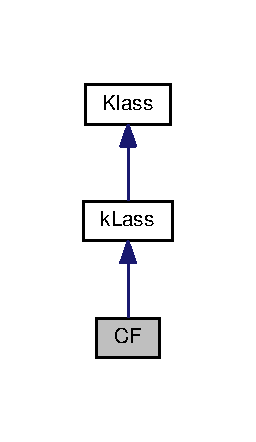
\includegraphics[width=123pt]{class_k_1_1_c_f__inherit__graph}
\end{center}
\end{figure}


Collaboration diagram for CF\+:
\nopagebreak
\begin{figure}[H]
\begin{center}
\leavevmode
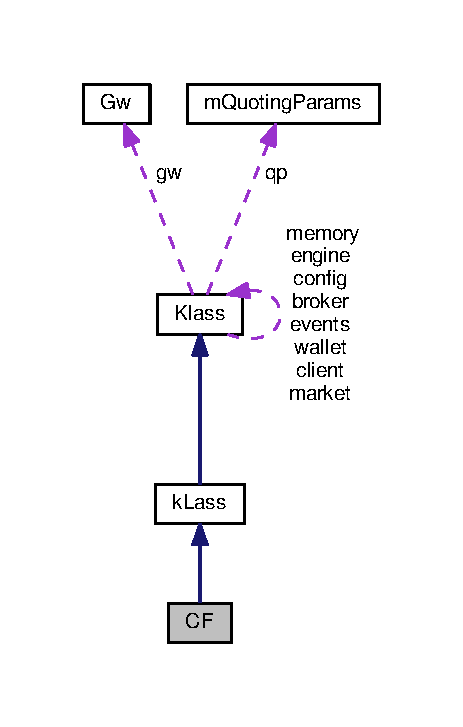
\includegraphics[width=222pt]{class_k_1_1_c_f__coll__graph}
\end{center}
\end{figure}
\subsection*{Public Member Functions}
\begin{DoxyCompactItemize}
\item 
\hyperlink{class_k_1_1_c_f_a5958a0f9f5083d45c036b0180ca70ebb}{CF} ()
\end{DoxyCompactItemize}
\subsection*{Data Fields}
\begin{DoxyCompactItemize}
\item 
int \hyperlink{class_k_1_1_c_f_ad8e21fbf694230c7356085f6a4c33946}{arg\+Port} = 3000
\item 
int \hyperlink{class_k_1_1_c_f_a4a280cd3b15e44c13dd04b093185f3d4}{arg\+Colors} = 0
\item 
int \hyperlink{class_k_1_1_c_f_adf3bd2e6fb3d053f4fbeb11b358355e7}{arg\+Debug} = 0
\item 
int \hyperlink{class_k_1_1_c_f_ab49089fd0430e11c5523a6266bcdeffb}{arg\+Debug\+Secret} = 0
\item 
int \hyperlink{class_k_1_1_c_f_a1d898d118f79784dbc862a2e89569b67}{arg\+Debug\+Events} = 0
\item 
int \hyperlink{class_k_1_1_c_f_a2573f341e6f95ab629a7ecefe25b657e}{arg\+Debug\+Orders} = 0
\item 
int \hyperlink{class_k_1_1_c_f_a7899599cb07687ad7b516452524f1ca0}{arg\+Debug\+Quotes} = 0
\item 
int \hyperlink{class_k_1_1_c_f_a15dc35f4e159f3ba1a145a89eef7ac46}{arg\+Debug\+Wallet} = 0
\item 
int \hyperlink{class_k_1_1_c_f_a71b0bc0bf8c0ade7768ed08a3163ae0b}{arg\+Without\+S\+SL} = 0
\item 
int \hyperlink{class_k_1_1_c_f_a4f93aa825293f552b554aa0f75eba23f}{arg\+Headless} = 0
\item 
int \hyperlink{class_k_1_1_c_f_a7a0670a55b62f58567ce174c4e2e7014}{arg\+Dustybot} = 0
\item 
int \hyperlink{class_k_1_1_c_f_acbb9fc24d192987c8caf829bfc12bec5}{arg\+Lifetime} = 0
\item 
int \hyperlink{class_k_1_1_c_f_ac2e0f5f7736fa94e4ae19da2bc1d9351}{arg\+Autobot} = 0
\item 
int \hyperlink{class_k_1_1_c_f_a3717f53c2ee309adbb6eec21c1d162c4}{arg\+Naked} = 0
\item 
int \hyperlink{class_k_1_1_c_f_a41db2c0e2e4ceca1dfff39f0ba30d72e}{arg\+Free} = 0
\item 
int \hyperlink{class_k_1_1_c_f_aa34daf182d57defef5e7f4557fff68e6}{arg\+Ignore\+Sun} = 0
\item 
int \hyperlink{class_k_1_1_c_f_a5aa7cca99b139409412af69133db10b1}{arg\+Ignore\+Moon} = 0
\item 
int \hyperlink{class_k_1_1_c_f_ab055f0fe04365bf08537040c5ba9d3ef}{arg\+Max\+Levels} = 0
\item 
int \hyperlink{class_k_1_1_c_f_a470f837189c8cb88935532c65444c298}{arg\+Test\+Chamber} = 0
\item 
\hyperlink{km_8h_ad4d00888c55a47a8a40ed8020d176086}{m\+Amount} \hyperlink{class_k_1_1_c_f_a6ba243e087d2134aa546907459589dbb}{arg\+Max\+Wallet} = 0
\item 
\hyperlink{km_8h_a392f9b7f384aa3539bbb890b059f5b8c}{m\+Price} \hyperlink{class_k_1_1_c_f_a62ca6f9cc06fae85d045ddb3b452b0d7}{arg\+Ewma\+U\+Short} = 0
\item 
\hyperlink{km_8h_a392f9b7f384aa3539bbb890b059f5b8c}{m\+Price} \hyperlink{class_k_1_1_c_f_a456df187a38686bcf173a862674b25ed}{arg\+Ewma\+X\+Short} = 0
\item 
\hyperlink{km_8h_a392f9b7f384aa3539bbb890b059f5b8c}{m\+Price} \hyperlink{class_k_1_1_c_f_aa863f101457aeab235daf34a708dd186}{arg\+Ewma\+Short} = 0
\item 
\hyperlink{km_8h_a392f9b7f384aa3539bbb890b059f5b8c}{m\+Price} \hyperlink{class_k_1_1_c_f_a33148205e367f7baa36de43f6c2b54d1}{arg\+Ewma\+Medium} = 0
\item 
\hyperlink{km_8h_a392f9b7f384aa3539bbb890b059f5b8c}{m\+Price} \hyperlink{class_k_1_1_c_f_a542c9f055f8a89a6fb9963d750be3417}{arg\+Ewma\+Long} = 0
\item 
\hyperlink{km_8h_a392f9b7f384aa3539bbb890b059f5b8c}{m\+Price} \hyperlink{class_k_1_1_c_f_a31294e3847b4d176d0b67dfc500fe268}{arg\+Ewma\+Very\+Long} = 0
\item 
string \hyperlink{class_k_1_1_c_f_ad88b2c38f30af5bfb88ddec1e06b6ead}{arg\+Title} = \char`\"{}K.\+sh\char`\"{}
\item 
string \hyperlink{class_k_1_1_c_f_a9e868129a03788dd992ba0e7548a6ea9}{arg\+Matryoshka} = \char`\"{}https\+://www.\+example.\+com/\char`\"{}
\item 
string \hyperlink{class_k_1_1_c_f_a892f38e1aca5d77e44a7b21f70710ebe}{arg\+User} = \char`\"{}N\+U\+LL\char`\"{}
\item 
string \hyperlink{class_k_1_1_c_f_a362e285d551ece07b51b724e25a7bc68}{arg\+Pass} = \char`\"{}N\+U\+LL\char`\"{}
\item 
string \hyperlink{class_k_1_1_c_f_ac2c90c943260d1f24bb92efa33e2f7ff}{arg\+Exchange} = \char`\"{}N\+U\+LL\char`\"{}
\item 
string \hyperlink{class_k_1_1_c_f_a8c9947131171d2d20bc1ea5b3423a395}{arg\+Currency} = \char`\"{}N\+U\+LL\char`\"{}
\item 
string \hyperlink{class_k_1_1_c_f_a88cf02a0929b4bc9d403c64fc0635d8e}{arg\+Apikey} = \char`\"{}N\+U\+LL\char`\"{}
\item 
string \hyperlink{class_k_1_1_c_f_a7f00f6255755b37220ad45131ae0ad28}{arg\+Secret} = \char`\"{}N\+U\+LL\char`\"{}
\item 
string \hyperlink{class_k_1_1_c_f_a330672ad82dc3b07df05e5515d1bc0c1}{arg\+Username} = \char`\"{}N\+U\+LL\char`\"{}
\item 
string \hyperlink{class_k_1_1_c_f_aab55dec94bd05605b7931510960734b6}{arg\+Passphrase} = \char`\"{}N\+U\+LL\char`\"{}
\item 
string \hyperlink{class_k_1_1_c_f_aa00ec893e8f2756c08b219b8ef6ccad8}{arg\+Http} = \char`\"{}N\+U\+LL\char`\"{}
\item 
string \hyperlink{class_k_1_1_c_f_ab6402172f1adc2b82968e480816c5df8}{arg\+Wss} = \char`\"{}N\+U\+LL\char`\"{}
\item 
string \hyperlink{class_k_1_1_c_f_a1554afb0c30eb312e1b19b476b9bed36}{arg\+Database} = \char`\"{}\char`\"{}
\item 
string \hyperlink{class_k_1_1_c_f_a82308ee2afc2d7517b4067a23e783b49}{arg\+Diskdata} = \char`\"{}\char`\"{}
\item 
string \hyperlink{class_k_1_1_c_f_a007fd80e3d8d6bc1f57ce7fb36e6f7e7}{arg\+Whitelist} = \char`\"{}\char`\"{}
\end{DoxyCompactItemize}
\subsection*{Protected Member Functions}
\begin{DoxyCompactItemize}
\item 
void \hyperlink{class_k_1_1_c_f_aa7590ffe947041a741bb86945e1aa572}{load} (int argc, char $\ast$$\ast$argv)
\item 
void \hyperlink{class_k_1_1_c_f_a13a43e6d814de94978c515cb084873b1}{run} ()
\end{DoxyCompactItemize}
\subsection*{Additional Inherited Members}


\subsection{Detailed Description}


Definition at line 5 of file cf.\+h.



\subsection{Constructor \& Destructor Documentation}
\index{K\+::\+CF@{K\+::\+CF}!CF@{CF}}
\index{CF@{CF}!K\+::\+CF@{K\+::\+CF}}
\subsubsection[{\texorpdfstring{C\+F()}{CF()}}]{\setlength{\rightskip}{0pt plus 5cm}{\bf CF} (
\begin{DoxyParamCaption}
{}
\end{DoxyParamCaption}
)\hspace{0.3cm}{\ttfamily [inline]}}\hypertarget{class_k_1_1_c_f_a5958a0f9f5083d45c036b0180ca70ebb}{}\label{class_k_1_1_c_f_a5958a0f9f5083d45c036b0180ca70ebb}


Definition at line 26 of file cf.\+h.



\subsection{Member Function Documentation}
\index{K\+::\+CF@{K\+::\+CF}!load@{load}}
\index{load@{load}!K\+::\+CF@{K\+::\+CF}}
\subsubsection[{\texorpdfstring{load(int argc, char $\ast$$\ast$argv)}{load(int argc, char **argv)}}]{\setlength{\rightskip}{0pt plus 5cm}void load (
\begin{DoxyParamCaption}
\item[{int}]{argc, }
\item[{char $\ast$$\ast$}]{argv}
\end{DoxyParamCaption}
)\hspace{0.3cm}{\ttfamily [inline]}, {\ttfamily [protected]}, {\ttfamily [virtual]}}\hypertarget{class_k_1_1_c_f_aa7590ffe947041a741bb86945e1aa572}{}\label{class_k_1_1_c_f_aa7590ffe947041a741bb86945e1aa572}


Reimplemented from \hyperlink{class_k_1_1_klass_af62dc66ce38ed384a91677aa1485eb1f}{Klass}.



Definition at line 30 of file cf.\+h.

\index{K\+::\+CF@{K\+::\+CF}!run@{run}}
\index{run@{run}!K\+::\+CF@{K\+::\+CF}}
\subsubsection[{\texorpdfstring{run()}{run()}}]{\setlength{\rightskip}{0pt plus 5cm}void run (
\begin{DoxyParamCaption}
{}
\end{DoxyParamCaption}
)\hspace{0.3cm}{\ttfamily [inline]}, {\ttfamily [protected]}, {\ttfamily [virtual]}}\hypertarget{class_k_1_1_c_f_a13a43e6d814de94978c515cb084873b1}{}\label{class_k_1_1_c_f_a13a43e6d814de94978c515cb084873b1}


Reimplemented from \hyperlink{class_k_1_1_klass_a72fcb26a14f6beb1c3fbace9ab3e7dbb}{Klass}.



Definition at line 201 of file cf.\+h.



\subsection{Field Documentation}
\index{K\+::\+CF@{K\+::\+CF}!arg\+Apikey@{arg\+Apikey}}
\index{arg\+Apikey@{arg\+Apikey}!K\+::\+CF@{K\+::\+CF}}
\subsubsection[{\texorpdfstring{arg\+Apikey}{argApikey}}]{\setlength{\rightskip}{0pt plus 5cm}string arg\+Apikey = \char`\"{}N\+U\+LL\char`\"{}}\hypertarget{class_k_1_1_c_f_a88cf02a0929b4bc9d403c64fc0635d8e}{}\label{class_k_1_1_c_f_a88cf02a0929b4bc9d403c64fc0635d8e}


Definition at line 20 of file cf.\+h.

\index{K\+::\+CF@{K\+::\+CF}!arg\+Autobot@{arg\+Autobot}}
\index{arg\+Autobot@{arg\+Autobot}!K\+::\+CF@{K\+::\+CF}}
\subsubsection[{\texorpdfstring{arg\+Autobot}{argAutobot}}]{\setlength{\rightskip}{0pt plus 5cm}int arg\+Autobot = 0}\hypertarget{class_k_1_1_c_f_ac2e0f5f7736fa94e4ae19da2bc1d9351}{}\label{class_k_1_1_c_f_ac2e0f5f7736fa94e4ae19da2bc1d9351}


Definition at line 11 of file cf.\+h.

\index{K\+::\+CF@{K\+::\+CF}!arg\+Colors@{arg\+Colors}}
\index{arg\+Colors@{arg\+Colors}!K\+::\+CF@{K\+::\+CF}}
\subsubsection[{\texorpdfstring{arg\+Colors}{argColors}}]{\setlength{\rightskip}{0pt plus 5cm}int arg\+Colors = 0}\hypertarget{class_k_1_1_c_f_a4a280cd3b15e44c13dd04b093185f3d4}{}\label{class_k_1_1_c_f_a4a280cd3b15e44c13dd04b093185f3d4}


Definition at line 7 of file cf.\+h.

\index{K\+::\+CF@{K\+::\+CF}!arg\+Currency@{arg\+Currency}}
\index{arg\+Currency@{arg\+Currency}!K\+::\+CF@{K\+::\+CF}}
\subsubsection[{\texorpdfstring{arg\+Currency}{argCurrency}}]{\setlength{\rightskip}{0pt plus 5cm}string arg\+Currency = \char`\"{}N\+U\+LL\char`\"{}}\hypertarget{class_k_1_1_c_f_a8c9947131171d2d20bc1ea5b3423a395}{}\label{class_k_1_1_c_f_a8c9947131171d2d20bc1ea5b3423a395}


Definition at line 19 of file cf.\+h.

\index{K\+::\+CF@{K\+::\+CF}!arg\+Database@{arg\+Database}}
\index{arg\+Database@{arg\+Database}!K\+::\+CF@{K\+::\+CF}}
\subsubsection[{\texorpdfstring{arg\+Database}{argDatabase}}]{\setlength{\rightskip}{0pt plus 5cm}string arg\+Database = \char`\"{}\char`\"{}}\hypertarget{class_k_1_1_c_f_a1554afb0c30eb312e1b19b476b9bed36}{}\label{class_k_1_1_c_f_a1554afb0c30eb312e1b19b476b9bed36}


Definition at line 23 of file cf.\+h.

\index{K\+::\+CF@{K\+::\+CF}!arg\+Debug@{arg\+Debug}}
\index{arg\+Debug@{arg\+Debug}!K\+::\+CF@{K\+::\+CF}}
\subsubsection[{\texorpdfstring{arg\+Debug}{argDebug}}]{\setlength{\rightskip}{0pt plus 5cm}int arg\+Debug = 0}\hypertarget{class_k_1_1_c_f_adf3bd2e6fb3d053f4fbeb11b358355e7}{}\label{class_k_1_1_c_f_adf3bd2e6fb3d053f4fbeb11b358355e7}


Definition at line 7 of file cf.\+h.

\index{K\+::\+CF@{K\+::\+CF}!arg\+Debug\+Events@{arg\+Debug\+Events}}
\index{arg\+Debug\+Events@{arg\+Debug\+Events}!K\+::\+CF@{K\+::\+CF}}
\subsubsection[{\texorpdfstring{arg\+Debug\+Events}{argDebugEvents}}]{\setlength{\rightskip}{0pt plus 5cm}int arg\+Debug\+Events = 0}\hypertarget{class_k_1_1_c_f_a1d898d118f79784dbc862a2e89569b67}{}\label{class_k_1_1_c_f_a1d898d118f79784dbc862a2e89569b67}


Definition at line 8 of file cf.\+h.

\index{K\+::\+CF@{K\+::\+CF}!arg\+Debug\+Orders@{arg\+Debug\+Orders}}
\index{arg\+Debug\+Orders@{arg\+Debug\+Orders}!K\+::\+CF@{K\+::\+CF}}
\subsubsection[{\texorpdfstring{arg\+Debug\+Orders}{argDebugOrders}}]{\setlength{\rightskip}{0pt plus 5cm}int arg\+Debug\+Orders = 0}\hypertarget{class_k_1_1_c_f_a2573f341e6f95ab629a7ecefe25b657e}{}\label{class_k_1_1_c_f_a2573f341e6f95ab629a7ecefe25b657e}


Definition at line 8 of file cf.\+h.

\index{K\+::\+CF@{K\+::\+CF}!arg\+Debug\+Quotes@{arg\+Debug\+Quotes}}
\index{arg\+Debug\+Quotes@{arg\+Debug\+Quotes}!K\+::\+CF@{K\+::\+CF}}
\subsubsection[{\texorpdfstring{arg\+Debug\+Quotes}{argDebugQuotes}}]{\setlength{\rightskip}{0pt plus 5cm}int arg\+Debug\+Quotes = 0}\hypertarget{class_k_1_1_c_f_a7899599cb07687ad7b516452524f1ca0}{}\label{class_k_1_1_c_f_a7899599cb07687ad7b516452524f1ca0}


Definition at line 9 of file cf.\+h.

\index{K\+::\+CF@{K\+::\+CF}!arg\+Debug\+Secret@{arg\+Debug\+Secret}}
\index{arg\+Debug\+Secret@{arg\+Debug\+Secret}!K\+::\+CF@{K\+::\+CF}}
\subsubsection[{\texorpdfstring{arg\+Debug\+Secret}{argDebugSecret}}]{\setlength{\rightskip}{0pt plus 5cm}int arg\+Debug\+Secret = 0}\hypertarget{class_k_1_1_c_f_ab49089fd0430e11c5523a6266bcdeffb}{}\label{class_k_1_1_c_f_ab49089fd0430e11c5523a6266bcdeffb}


Definition at line 8 of file cf.\+h.

\index{K\+::\+CF@{K\+::\+CF}!arg\+Debug\+Wallet@{arg\+Debug\+Wallet}}
\index{arg\+Debug\+Wallet@{arg\+Debug\+Wallet}!K\+::\+CF@{K\+::\+CF}}
\subsubsection[{\texorpdfstring{arg\+Debug\+Wallet}{argDebugWallet}}]{\setlength{\rightskip}{0pt plus 5cm}int arg\+Debug\+Wallet = 0}\hypertarget{class_k_1_1_c_f_a15dc35f4e159f3ba1a145a89eef7ac46}{}\label{class_k_1_1_c_f_a15dc35f4e159f3ba1a145a89eef7ac46}


Definition at line 9 of file cf.\+h.

\index{K\+::\+CF@{K\+::\+CF}!arg\+Diskdata@{arg\+Diskdata}}
\index{arg\+Diskdata@{arg\+Diskdata}!K\+::\+CF@{K\+::\+CF}}
\subsubsection[{\texorpdfstring{arg\+Diskdata}{argDiskdata}}]{\setlength{\rightskip}{0pt plus 5cm}string arg\+Diskdata = \char`\"{}\char`\"{}}\hypertarget{class_k_1_1_c_f_a82308ee2afc2d7517b4067a23e783b49}{}\label{class_k_1_1_c_f_a82308ee2afc2d7517b4067a23e783b49}


Definition at line 23 of file cf.\+h.

\index{K\+::\+CF@{K\+::\+CF}!arg\+Dustybot@{arg\+Dustybot}}
\index{arg\+Dustybot@{arg\+Dustybot}!K\+::\+CF@{K\+::\+CF}}
\subsubsection[{\texorpdfstring{arg\+Dustybot}{argDustybot}}]{\setlength{\rightskip}{0pt plus 5cm}int arg\+Dustybot = 0}\hypertarget{class_k_1_1_c_f_a7a0670a55b62f58567ce174c4e2e7014}{}\label{class_k_1_1_c_f_a7a0670a55b62f58567ce174c4e2e7014}


Definition at line 10 of file cf.\+h.

\index{K\+::\+CF@{K\+::\+CF}!arg\+Ewma\+Long@{arg\+Ewma\+Long}}
\index{arg\+Ewma\+Long@{arg\+Ewma\+Long}!K\+::\+CF@{K\+::\+CF}}
\subsubsection[{\texorpdfstring{arg\+Ewma\+Long}{argEwmaLong}}]{\setlength{\rightskip}{0pt plus 5cm}{\bf m\+Price} arg\+Ewma\+Long = 0}\hypertarget{class_k_1_1_c_f_a542c9f055f8a89a6fb9963d750be3417}{}\label{class_k_1_1_c_f_a542c9f055f8a89a6fb9963d750be3417}


Definition at line 16 of file cf.\+h.

\index{K\+::\+CF@{K\+::\+CF}!arg\+Ewma\+Medium@{arg\+Ewma\+Medium}}
\index{arg\+Ewma\+Medium@{arg\+Ewma\+Medium}!K\+::\+CF@{K\+::\+CF}}
\subsubsection[{\texorpdfstring{arg\+Ewma\+Medium}{argEwmaMedium}}]{\setlength{\rightskip}{0pt plus 5cm}{\bf m\+Price} arg\+Ewma\+Medium = 0}\hypertarget{class_k_1_1_c_f_a33148205e367f7baa36de43f6c2b54d1}{}\label{class_k_1_1_c_f_a33148205e367f7baa36de43f6c2b54d1}


Definition at line 16 of file cf.\+h.

\index{K\+::\+CF@{K\+::\+CF}!arg\+Ewma\+Short@{arg\+Ewma\+Short}}
\index{arg\+Ewma\+Short@{arg\+Ewma\+Short}!K\+::\+CF@{K\+::\+CF}}
\subsubsection[{\texorpdfstring{arg\+Ewma\+Short}{argEwmaShort}}]{\setlength{\rightskip}{0pt plus 5cm}{\bf m\+Price} arg\+Ewma\+Short = 0}\hypertarget{class_k_1_1_c_f_aa863f101457aeab235daf34a708dd186}{}\label{class_k_1_1_c_f_aa863f101457aeab235daf34a708dd186}


Definition at line 15 of file cf.\+h.

\index{K\+::\+CF@{K\+::\+CF}!arg\+Ewma\+U\+Short@{arg\+Ewma\+U\+Short}}
\index{arg\+Ewma\+U\+Short@{arg\+Ewma\+U\+Short}!K\+::\+CF@{K\+::\+CF}}
\subsubsection[{\texorpdfstring{arg\+Ewma\+U\+Short}{argEwmaUShort}}]{\setlength{\rightskip}{0pt plus 5cm}{\bf m\+Price} arg\+Ewma\+U\+Short = 0}\hypertarget{class_k_1_1_c_f_a62ca6f9cc06fae85d045ddb3b452b0d7}{}\label{class_k_1_1_c_f_a62ca6f9cc06fae85d045ddb3b452b0d7}


Definition at line 15 of file cf.\+h.

\index{K\+::\+CF@{K\+::\+CF}!arg\+Ewma\+Very\+Long@{arg\+Ewma\+Very\+Long}}
\index{arg\+Ewma\+Very\+Long@{arg\+Ewma\+Very\+Long}!K\+::\+CF@{K\+::\+CF}}
\subsubsection[{\texorpdfstring{arg\+Ewma\+Very\+Long}{argEwmaVeryLong}}]{\setlength{\rightskip}{0pt plus 5cm}{\bf m\+Price} arg\+Ewma\+Very\+Long = 0}\hypertarget{class_k_1_1_c_f_a31294e3847b4d176d0b67dfc500fe268}{}\label{class_k_1_1_c_f_a31294e3847b4d176d0b67dfc500fe268}


Definition at line 16 of file cf.\+h.

\index{K\+::\+CF@{K\+::\+CF}!arg\+Ewma\+X\+Short@{arg\+Ewma\+X\+Short}}
\index{arg\+Ewma\+X\+Short@{arg\+Ewma\+X\+Short}!K\+::\+CF@{K\+::\+CF}}
\subsubsection[{\texorpdfstring{arg\+Ewma\+X\+Short}{argEwmaXShort}}]{\setlength{\rightskip}{0pt plus 5cm}{\bf m\+Price} arg\+Ewma\+X\+Short = 0}\hypertarget{class_k_1_1_c_f_a456df187a38686bcf173a862674b25ed}{}\label{class_k_1_1_c_f_a456df187a38686bcf173a862674b25ed}


Definition at line 15 of file cf.\+h.

\index{K\+::\+CF@{K\+::\+CF}!arg\+Exchange@{arg\+Exchange}}
\index{arg\+Exchange@{arg\+Exchange}!K\+::\+CF@{K\+::\+CF}}
\subsubsection[{\texorpdfstring{arg\+Exchange}{argExchange}}]{\setlength{\rightskip}{0pt plus 5cm}string arg\+Exchange = \char`\"{}N\+U\+LL\char`\"{}}\hypertarget{class_k_1_1_c_f_ac2c90c943260d1f24bb92efa33e2f7ff}{}\label{class_k_1_1_c_f_ac2c90c943260d1f24bb92efa33e2f7ff}


Definition at line 19 of file cf.\+h.

\index{K\+::\+CF@{K\+::\+CF}!arg\+Free@{arg\+Free}}
\index{arg\+Free@{arg\+Free}!K\+::\+CF@{K\+::\+CF}}
\subsubsection[{\texorpdfstring{arg\+Free}{argFree}}]{\setlength{\rightskip}{0pt plus 5cm}int arg\+Free = 0}\hypertarget{class_k_1_1_c_f_a41db2c0e2e4ceca1dfff39f0ba30d72e}{}\label{class_k_1_1_c_f_a41db2c0e2e4ceca1dfff39f0ba30d72e}


Definition at line 11 of file cf.\+h.

\index{K\+::\+CF@{K\+::\+CF}!arg\+Headless@{arg\+Headless}}
\index{arg\+Headless@{arg\+Headless}!K\+::\+CF@{K\+::\+CF}}
\subsubsection[{\texorpdfstring{arg\+Headless}{argHeadless}}]{\setlength{\rightskip}{0pt plus 5cm}int arg\+Headless = 0}\hypertarget{class_k_1_1_c_f_a4f93aa825293f552b554aa0f75eba23f}{}\label{class_k_1_1_c_f_a4f93aa825293f552b554aa0f75eba23f}


Definition at line 10 of file cf.\+h.

\index{K\+::\+CF@{K\+::\+CF}!arg\+Http@{arg\+Http}}
\index{arg\+Http@{arg\+Http}!K\+::\+CF@{K\+::\+CF}}
\subsubsection[{\texorpdfstring{arg\+Http}{argHttp}}]{\setlength{\rightskip}{0pt plus 5cm}string arg\+Http = \char`\"{}N\+U\+LL\char`\"{}}\hypertarget{class_k_1_1_c_f_aa00ec893e8f2756c08b219b8ef6ccad8}{}\label{class_k_1_1_c_f_aa00ec893e8f2756c08b219b8ef6ccad8}


Definition at line 22 of file cf.\+h.

\index{K\+::\+CF@{K\+::\+CF}!arg\+Ignore\+Moon@{arg\+Ignore\+Moon}}
\index{arg\+Ignore\+Moon@{arg\+Ignore\+Moon}!K\+::\+CF@{K\+::\+CF}}
\subsubsection[{\texorpdfstring{arg\+Ignore\+Moon}{argIgnoreMoon}}]{\setlength{\rightskip}{0pt plus 5cm}int arg\+Ignore\+Moon = 0}\hypertarget{class_k_1_1_c_f_a5aa7cca99b139409412af69133db10b1}{}\label{class_k_1_1_c_f_a5aa7cca99b139409412af69133db10b1}


Definition at line 12 of file cf.\+h.

\index{K\+::\+CF@{K\+::\+CF}!arg\+Ignore\+Sun@{arg\+Ignore\+Sun}}
\index{arg\+Ignore\+Sun@{arg\+Ignore\+Sun}!K\+::\+CF@{K\+::\+CF}}
\subsubsection[{\texorpdfstring{arg\+Ignore\+Sun}{argIgnoreSun}}]{\setlength{\rightskip}{0pt plus 5cm}int arg\+Ignore\+Sun = 0}\hypertarget{class_k_1_1_c_f_aa34daf182d57defef5e7f4557fff68e6}{}\label{class_k_1_1_c_f_aa34daf182d57defef5e7f4557fff68e6}


Definition at line 12 of file cf.\+h.

\index{K\+::\+CF@{K\+::\+CF}!arg\+Lifetime@{arg\+Lifetime}}
\index{arg\+Lifetime@{arg\+Lifetime}!K\+::\+CF@{K\+::\+CF}}
\subsubsection[{\texorpdfstring{arg\+Lifetime}{argLifetime}}]{\setlength{\rightskip}{0pt plus 5cm}int arg\+Lifetime = 0}\hypertarget{class_k_1_1_c_f_acbb9fc24d192987c8caf829bfc12bec5}{}\label{class_k_1_1_c_f_acbb9fc24d192987c8caf829bfc12bec5}


Definition at line 10 of file cf.\+h.

\index{K\+::\+CF@{K\+::\+CF}!arg\+Matryoshka@{arg\+Matryoshka}}
\index{arg\+Matryoshka@{arg\+Matryoshka}!K\+::\+CF@{K\+::\+CF}}
\subsubsection[{\texorpdfstring{arg\+Matryoshka}{argMatryoshka}}]{\setlength{\rightskip}{0pt plus 5cm}string arg\+Matryoshka = \char`\"{}https\+://www.\+example.\+com/\char`\"{}}\hypertarget{class_k_1_1_c_f_a9e868129a03788dd992ba0e7548a6ea9}{}\label{class_k_1_1_c_f_a9e868129a03788dd992ba0e7548a6ea9}


Definition at line 17 of file cf.\+h.

\index{K\+::\+CF@{K\+::\+CF}!arg\+Max\+Levels@{arg\+Max\+Levels}}
\index{arg\+Max\+Levels@{arg\+Max\+Levels}!K\+::\+CF@{K\+::\+CF}}
\subsubsection[{\texorpdfstring{arg\+Max\+Levels}{argMaxLevels}}]{\setlength{\rightskip}{0pt plus 5cm}int arg\+Max\+Levels = 0}\hypertarget{class_k_1_1_c_f_ab055f0fe04365bf08537040c5ba9d3ef}{}\label{class_k_1_1_c_f_ab055f0fe04365bf08537040c5ba9d3ef}


Definition at line 12 of file cf.\+h.

\index{K\+::\+CF@{K\+::\+CF}!arg\+Max\+Wallet@{arg\+Max\+Wallet}}
\index{arg\+Max\+Wallet@{arg\+Max\+Wallet}!K\+::\+CF@{K\+::\+CF}}
\subsubsection[{\texorpdfstring{arg\+Max\+Wallet}{argMaxWallet}}]{\setlength{\rightskip}{0pt plus 5cm}{\bf m\+Amount} arg\+Max\+Wallet = 0}\hypertarget{class_k_1_1_c_f_a6ba243e087d2134aa546907459589dbb}{}\label{class_k_1_1_c_f_a6ba243e087d2134aa546907459589dbb}


Definition at line 14 of file cf.\+h.

\index{K\+::\+CF@{K\+::\+CF}!arg\+Naked@{arg\+Naked}}
\index{arg\+Naked@{arg\+Naked}!K\+::\+CF@{K\+::\+CF}}
\subsubsection[{\texorpdfstring{arg\+Naked}{argNaked}}]{\setlength{\rightskip}{0pt plus 5cm}int arg\+Naked = 0}\hypertarget{class_k_1_1_c_f_a3717f53c2ee309adbb6eec21c1d162c4}{}\label{class_k_1_1_c_f_a3717f53c2ee309adbb6eec21c1d162c4}


Definition at line 11 of file cf.\+h.

\index{K\+::\+CF@{K\+::\+CF}!arg\+Pass@{arg\+Pass}}
\index{arg\+Pass@{arg\+Pass}!K\+::\+CF@{K\+::\+CF}}
\subsubsection[{\texorpdfstring{arg\+Pass}{argPass}}]{\setlength{\rightskip}{0pt plus 5cm}string arg\+Pass = \char`\"{}N\+U\+LL\char`\"{}}\hypertarget{class_k_1_1_c_f_a362e285d551ece07b51b724e25a7bc68}{}\label{class_k_1_1_c_f_a362e285d551ece07b51b724e25a7bc68}


Definition at line 18 of file cf.\+h.

\index{K\+::\+CF@{K\+::\+CF}!arg\+Passphrase@{arg\+Passphrase}}
\index{arg\+Passphrase@{arg\+Passphrase}!K\+::\+CF@{K\+::\+CF}}
\subsubsection[{\texorpdfstring{arg\+Passphrase}{argPassphrase}}]{\setlength{\rightskip}{0pt plus 5cm}string arg\+Passphrase = \char`\"{}N\+U\+LL\char`\"{}}\hypertarget{class_k_1_1_c_f_aab55dec94bd05605b7931510960734b6}{}\label{class_k_1_1_c_f_aab55dec94bd05605b7931510960734b6}


Definition at line 21 of file cf.\+h.

\index{K\+::\+CF@{K\+::\+CF}!arg\+Port@{arg\+Port}}
\index{arg\+Port@{arg\+Port}!K\+::\+CF@{K\+::\+CF}}
\subsubsection[{\texorpdfstring{arg\+Port}{argPort}}]{\setlength{\rightskip}{0pt plus 5cm}int arg\+Port = 3000}\hypertarget{class_k_1_1_c_f_ad8e21fbf694230c7356085f6a4c33946}{}\label{class_k_1_1_c_f_ad8e21fbf694230c7356085f6a4c33946}


Definition at line 7 of file cf.\+h.

\index{K\+::\+CF@{K\+::\+CF}!arg\+Secret@{arg\+Secret}}
\index{arg\+Secret@{arg\+Secret}!K\+::\+CF@{K\+::\+CF}}
\subsubsection[{\texorpdfstring{arg\+Secret}{argSecret}}]{\setlength{\rightskip}{0pt plus 5cm}string arg\+Secret = \char`\"{}N\+U\+LL\char`\"{}}\hypertarget{class_k_1_1_c_f_a7f00f6255755b37220ad45131ae0ad28}{}\label{class_k_1_1_c_f_a7f00f6255755b37220ad45131ae0ad28}


Definition at line 20 of file cf.\+h.

\index{K\+::\+CF@{K\+::\+CF}!arg\+Test\+Chamber@{arg\+Test\+Chamber}}
\index{arg\+Test\+Chamber@{arg\+Test\+Chamber}!K\+::\+CF@{K\+::\+CF}}
\subsubsection[{\texorpdfstring{arg\+Test\+Chamber}{argTestChamber}}]{\setlength{\rightskip}{0pt plus 5cm}int arg\+Test\+Chamber = 0}\hypertarget{class_k_1_1_c_f_a470f837189c8cb88935532c65444c298}{}\label{class_k_1_1_c_f_a470f837189c8cb88935532c65444c298}


Definition at line 13 of file cf.\+h.

\index{K\+::\+CF@{K\+::\+CF}!arg\+Title@{arg\+Title}}
\index{arg\+Title@{arg\+Title}!K\+::\+CF@{K\+::\+CF}}
\subsubsection[{\texorpdfstring{arg\+Title}{argTitle}}]{\setlength{\rightskip}{0pt plus 5cm}string arg\+Title = \char`\"{}K.\+sh\char`\"{}}\hypertarget{class_k_1_1_c_f_ad88b2c38f30af5bfb88ddec1e06b6ead}{}\label{class_k_1_1_c_f_ad88b2c38f30af5bfb88ddec1e06b6ead}


Definition at line 17 of file cf.\+h.

\index{K\+::\+CF@{K\+::\+CF}!arg\+User@{arg\+User}}
\index{arg\+User@{arg\+User}!K\+::\+CF@{K\+::\+CF}}
\subsubsection[{\texorpdfstring{arg\+User}{argUser}}]{\setlength{\rightskip}{0pt plus 5cm}string arg\+User = \char`\"{}N\+U\+LL\char`\"{}}\hypertarget{class_k_1_1_c_f_a892f38e1aca5d77e44a7b21f70710ebe}{}\label{class_k_1_1_c_f_a892f38e1aca5d77e44a7b21f70710ebe}


Definition at line 18 of file cf.\+h.

\index{K\+::\+CF@{K\+::\+CF}!arg\+Username@{arg\+Username}}
\index{arg\+Username@{arg\+Username}!K\+::\+CF@{K\+::\+CF}}
\subsubsection[{\texorpdfstring{arg\+Username}{argUsername}}]{\setlength{\rightskip}{0pt plus 5cm}string arg\+Username = \char`\"{}N\+U\+LL\char`\"{}}\hypertarget{class_k_1_1_c_f_a330672ad82dc3b07df05e5515d1bc0c1}{}\label{class_k_1_1_c_f_a330672ad82dc3b07df05e5515d1bc0c1}


Definition at line 21 of file cf.\+h.

\index{K\+::\+CF@{K\+::\+CF}!arg\+Whitelist@{arg\+Whitelist}}
\index{arg\+Whitelist@{arg\+Whitelist}!K\+::\+CF@{K\+::\+CF}}
\subsubsection[{\texorpdfstring{arg\+Whitelist}{argWhitelist}}]{\setlength{\rightskip}{0pt plus 5cm}string arg\+Whitelist = \char`\"{}\char`\"{}}\hypertarget{class_k_1_1_c_f_a007fd80e3d8d6bc1f57ce7fb36e6f7e7}{}\label{class_k_1_1_c_f_a007fd80e3d8d6bc1f57ce7fb36e6f7e7}


Definition at line 24 of file cf.\+h.

\index{K\+::\+CF@{K\+::\+CF}!arg\+Without\+S\+SL@{arg\+Without\+S\+SL}}
\index{arg\+Without\+S\+SL@{arg\+Without\+S\+SL}!K\+::\+CF@{K\+::\+CF}}
\subsubsection[{\texorpdfstring{arg\+Without\+S\+SL}{argWithoutSSL}}]{\setlength{\rightskip}{0pt plus 5cm}int arg\+Without\+S\+SL = 0}\hypertarget{class_k_1_1_c_f_a71b0bc0bf8c0ade7768ed08a3163ae0b}{}\label{class_k_1_1_c_f_a71b0bc0bf8c0ade7768ed08a3163ae0b}


Definition at line 9 of file cf.\+h.

\index{K\+::\+CF@{K\+::\+CF}!arg\+Wss@{arg\+Wss}}
\index{arg\+Wss@{arg\+Wss}!K\+::\+CF@{K\+::\+CF}}
\subsubsection[{\texorpdfstring{arg\+Wss}{argWss}}]{\setlength{\rightskip}{0pt plus 5cm}string arg\+Wss = \char`\"{}N\+U\+LL\char`\"{}}\hypertarget{class_k_1_1_c_f_ab6402172f1adc2b82968e480816c5df8}{}\label{class_k_1_1_c_f_ab6402172f1adc2b82968e480816c5df8}


Definition at line 22 of file cf.\+h.



The documentation for this class was generated from the following file\+:\begin{DoxyCompactItemize}
\item 
\hyperlink{cf_8h}{cf.\+h}\end{DoxyCompactItemize}

\hypertarget{class_k_1_1_d_b}{}\section{DB Class Reference}
\label{class_k_1_1_d_b}\index{DB@{DB}}


{\ttfamily \#include $<$db.\+h$>$}



Inheritance diagram for DB\+:
\nopagebreak
\begin{figure}[H]
\begin{center}
\leavevmode
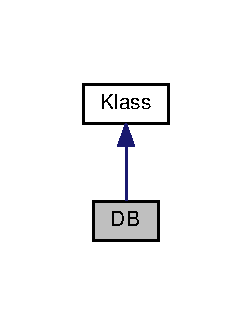
\includegraphics[width=121pt]{class_k_1_1_d_b__inherit__graph}
\end{center}
\end{figure}


Collaboration diagram for DB\+:
\nopagebreak
\begin{figure}[H]
\begin{center}
\leavevmode
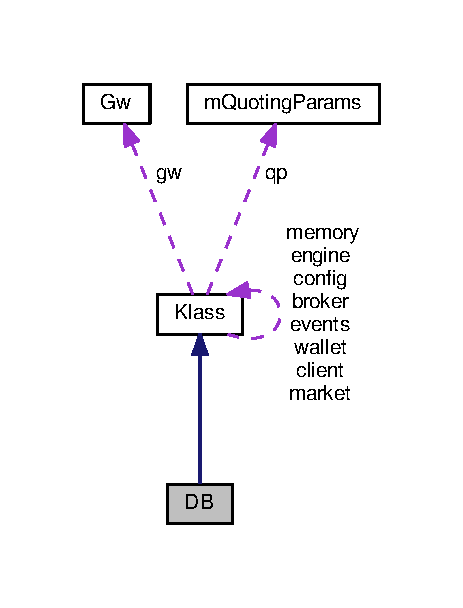
\includegraphics[width=222pt]{class_k_1_1_d_b__coll__graph}
\end{center}
\end{figure}
\subsection*{Public Member Functions}
\begin{DoxyCompactItemize}
\item 
json \hyperlink{class_k_1_1_d_b_a069b992af5564be9a2a200e810cc3dfd}{load} (const \hyperlink{namespace_k_a06e0333f0bcd3fc79835735bb9cda73d}{m\+Matter} \&table)
\item 
void \hyperlink{class_k_1_1_d_b_ad83cbb93689eee240577ca5f9c8cec07}{insert} (const \hyperlink{namespace_k_a06e0333f0bcd3fc79835735bb9cda73d}{m\+Matter} \&table, const json \&cell, const bool \&rm=true, const string \&update\+Id=\char`\"{}N\+U\+LL\char`\"{}, const \hyperlink{km_8h_ad02a70cba4c52ba2013e5e32ceaeac1c}{m\+Clock} \&rm\+Older=0)
\end{DoxyCompactItemize}
\subsection*{Data Fields}
\begin{DoxyCompactItemize}
\item 
function$<$ unsigned int()$>$ \hyperlink{class_k_1_1_d_b_a0101f5929df54174b492135ea931b3dc}{size} = \mbox{[}$\,$\mbox{]}() \{ return 0; \}
\end{DoxyCompactItemize}
\subsection*{Protected Member Functions}
\begin{DoxyCompactItemize}
\item 
void \hyperlink{class_k_1_1_d_b_a78f61ac2dd03bcba8e09ca20cd7d68e3}{load} ()
\item 
void \hyperlink{class_k_1_1_d_b_a13a43e6d814de94978c515cb084873b1}{run} ()
\end{DoxyCompactItemize}
\subsection*{Additional Inherited Members}


\subsection{Detailed Description}


Definition at line 7 of file db.\+h.



\subsection{Member Function Documentation}
\index{K\+::\+DB@{K\+::\+DB}!insert@{insert}}
\index{insert@{insert}!K\+::\+DB@{K\+::\+DB}}
\subsubsection[{\texorpdfstring{insert(const m\+Matter \&table, const json \&cell, const bool \&rm=true, const string \&update\+Id=""N\+U\+LL"", const m\+Clock \&rm\+Older=0)}{insert(const mMatter &table, const json &cell, const bool &rm=true, const string &updateId="NULL", const mClock &rmOlder=0)}}]{\setlength{\rightskip}{0pt plus 5cm}void insert (
\begin{DoxyParamCaption}
\item[{const {\bf m\+Matter} \&}]{table, }
\item[{const json \&}]{cell, }
\item[{const bool \&}]{rm = {\ttfamily true}, }
\item[{const string \&}]{update\+Id = {\ttfamily \char`\"{}NULL\char`\"{}}, }
\item[{const {\bf m\+Clock} \&}]{rm\+Older = {\ttfamily 0}}
\end{DoxyParamCaption}
)\hspace{0.3cm}{\ttfamily [inline]}}\hypertarget{class_k_1_1_d_b_ad83cbb93689eee240577ca5f9c8cec07}{}\label{class_k_1_1_d_b_ad83cbb93689eee240577ca5f9c8cec07}


Definition at line 39 of file db.\+h.

\index{K\+::\+DB@{K\+::\+DB}!load@{load}}
\index{load@{load}!K\+::\+DB@{K\+::\+DB}}
\subsubsection[{\texorpdfstring{load()}{load()}}]{\setlength{\rightskip}{0pt plus 5cm}void load (
\begin{DoxyParamCaption}
{}
\end{DoxyParamCaption}
)\hspace{0.3cm}{\ttfamily [inline]}, {\ttfamily [protected]}, {\ttfamily [virtual]}}\hypertarget{class_k_1_1_d_b_a78f61ac2dd03bcba8e09ca20cd7d68e3}{}\label{class_k_1_1_d_b_a78f61ac2dd03bcba8e09ca20cd7d68e3}


Reimplemented from \hyperlink{class_k_1_1_klass_a5588964fff1d1025245d134e159b60ee}{Klass}.



Definition at line 12 of file db.\+h.

\index{K\+::\+DB@{K\+::\+DB}!load@{load}}
\index{load@{load}!K\+::\+DB@{K\+::\+DB}}
\subsubsection[{\texorpdfstring{load(const m\+Matter \&table)}{load(const mMatter &table)}}]{\setlength{\rightskip}{0pt plus 5cm}json load (
\begin{DoxyParamCaption}
\item[{const {\bf m\+Matter} \&}]{table}
\end{DoxyParamCaption}
)\hspace{0.3cm}{\ttfamily [inline]}}\hypertarget{class_k_1_1_d_b_a069b992af5564be9a2a200e810cc3dfd}{}\label{class_k_1_1_d_b_a069b992af5564be9a2a200e810cc3dfd}


Definition at line 30 of file db.\+h.

\index{K\+::\+DB@{K\+::\+DB}!run@{run}}
\index{run@{run}!K\+::\+DB@{K\+::\+DB}}
\subsubsection[{\texorpdfstring{run()}{run()}}]{\setlength{\rightskip}{0pt plus 5cm}void run (
\begin{DoxyParamCaption}
{}
\end{DoxyParamCaption}
)\hspace{0.3cm}{\ttfamily [inline]}, {\ttfamily [protected]}, {\ttfamily [virtual]}}\hypertarget{class_k_1_1_d_b_a13a43e6d814de94978c515cb084873b1}{}\label{class_k_1_1_d_b_a13a43e6d814de94978c515cb084873b1}


Reimplemented from \hyperlink{class_k_1_1_klass_a72fcb26a14f6beb1c3fbace9ab3e7dbb}{Klass}.



Definition at line 21 of file db.\+h.



\subsection{Field Documentation}
\index{K\+::\+DB@{K\+::\+DB}!size@{size}}
\index{size@{size}!K\+::\+DB@{K\+::\+DB}}
\subsubsection[{\texorpdfstring{size}{size}}]{\setlength{\rightskip}{0pt plus 5cm}function$<$unsigned int()$>$ size = \mbox{[}$\,$\mbox{]}() \{ return 0; \}}\hypertarget{class_k_1_1_d_b_a0101f5929df54174b492135ea931b3dc}{}\label{class_k_1_1_d_b_a0101f5929df54174b492135ea931b3dc}


Definition at line 60 of file db.\+h.



The documentation for this class was generated from the following file\+:\begin{DoxyCompactItemize}
\item 
\hyperlink{db_8h}{db.\+h}\end{DoxyCompactItemize}

\hypertarget{class_k_1_1_e_v}{}\section{EV Class Reference}
\label{class_k_1_1_e_v}\index{EV@{EV}}


{\ttfamily \#include $<$ev.\+h$>$}



Inheritance diagram for EV\+:
\nopagebreak
\begin{figure}[H]
\begin{center}
\leavevmode
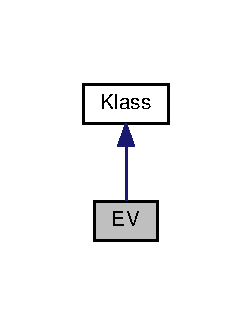
\includegraphics[width=121pt]{class_k_1_1_e_v__inherit__graph}
\end{center}
\end{figure}


Collaboration diagram for EV\+:
\nopagebreak
\begin{figure}[H]
\begin{center}
\leavevmode
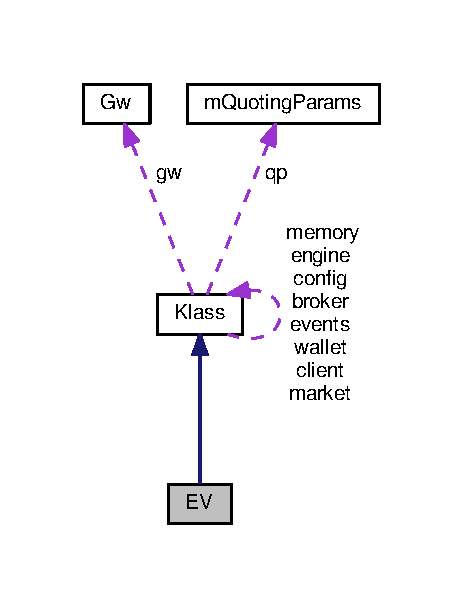
\includegraphics[width=222pt]{class_k_1_1_e_v__coll__graph}
\end{center}
\end{figure}
\subsection*{Public Member Functions}
\begin{DoxyCompactItemize}
\item 
void \hyperlink{class_k_1_1_e_v_a60de64d75454385b23995437f1d72669}{start} ()
\item 
void \hyperlink{class_k_1_1_e_v_a9b9c0a09ee1c1f71eed99acb7911d9af}{stop} (const function$<$ void()$>$ \&gw\+Cancel\+All)
\item 
void \hyperlink{class_k_1_1_e_v_a458bbe4cf81360301586b2e62a7f9dd2}{listen} ()
\item 
void \hyperlink{class_k_1_1_e_v_ab2cd59fade125e3516d94a02ce3b8579}{deferred} (const function$<$ void()$>$ \&fn)
\item 
void \hyperlink{class_k_1_1_e_v_aded8c7be8e73860a133e2f261c53b071}{async} (const function$<$ bool()$>$ \&fn)
\end{DoxyCompactItemize}
\subsection*{Data Fields}
\begin{DoxyCompactItemize}
\item 
u\+W\+S\+::\+Group$<$ u\+W\+S\+::\+S\+E\+R\+V\+ER $>$ $\ast$ \hyperlink{class_k_1_1_e_v_a9224c71ab6f6621adf6069f9c9adc751}{ui\+Group} = nullptr
\item 
Timer $\ast$ \hyperlink{class_k_1_1_e_v_a3528df0e9a2cf9a83ad1a92b6a79a5d4}{t\+Server} = nullptr
\item 
Timer $\ast$ \hyperlink{class_k_1_1_e_v_ae69ff430a805e08decf0feee8938b9b7}{t\+Client} = nullptr
\item 
function$<$ void(string)$>$ \hyperlink{class_k_1_1_e_v_ab04bc4fb6f845a182c6ee0a32c67550c}{debug}
\end{DoxyCompactItemize}
\subsection*{Protected Member Functions}
\begin{DoxyCompactItemize}
\item 
void \hyperlink{class_k_1_1_e_v_a78f61ac2dd03bcba8e09ca20cd7d68e3}{load} ()
\item 
void \hyperlink{class_k_1_1_e_v_aa9a0f090ee360e2a9f967200d30f4a22}{wait\+Data} ()
\item 
void \hyperlink{class_k_1_1_e_v_ade4c89163dbda531e71c8c75eb2868b4}{wait\+Time} ()
\item 
void \hyperlink{class_k_1_1_e_v_aa3f7b56799f5915cfbc902f6426c2bb2}{wait\+User} ()
\item 
void \hyperlink{class_k_1_1_e_v_a13a43e6d814de94978c515cb084873b1}{run} ()
\end{DoxyCompactItemize}
\subsection*{Additional Inherited Members}


\subsection{Detailed Description}


Definition at line 8 of file ev.\+h.



\subsection{Member Function Documentation}
\index{K\+::\+EV@{K\+::\+EV}!async@{async}}
\index{async@{async}!K\+::\+EV@{K\+::\+EV}}
\subsubsection[{\texorpdfstring{async(const function$<$ bool()$>$ \&fn)}{async(const function< bool()> &fn)}}]{\setlength{\rightskip}{0pt plus 5cm}void async (
\begin{DoxyParamCaption}
\item[{const function$<$ bool()$>$ \&}]{fn}
\end{DoxyParamCaption}
)\hspace{0.3cm}{\ttfamily [inline]}}\hypertarget{class_k_1_1_e_v_aded8c7be8e73860a133e2f261c53b071}{}\label{class_k_1_1_e_v_aded8c7be8e73860a133e2f261c53b071}


Definition at line 81 of file ev.\+h.

\index{K\+::\+EV@{K\+::\+EV}!deferred@{deferred}}
\index{deferred@{deferred}!K\+::\+EV@{K\+::\+EV}}
\subsubsection[{\texorpdfstring{deferred(const function$<$ void()$>$ \&fn)}{deferred(const function< void()> &fn)}}]{\setlength{\rightskip}{0pt plus 5cm}void deferred (
\begin{DoxyParamCaption}
\item[{const function$<$ void()$>$ \&}]{fn}
\end{DoxyParamCaption}
)\hspace{0.3cm}{\ttfamily [inline]}}\hypertarget{class_k_1_1_e_v_ab2cd59fade125e3516d94a02ce3b8579}{}\label{class_k_1_1_e_v_ab2cd59fade125e3516d94a02ce3b8579}


Definition at line 77 of file ev.\+h.

\index{K\+::\+EV@{K\+::\+EV}!listen@{listen}}
\index{listen@{listen}!K\+::\+EV@{K\+::\+EV}}
\subsubsection[{\texorpdfstring{listen()}{listen()}}]{\setlength{\rightskip}{0pt plus 5cm}void listen (
\begin{DoxyParamCaption}
{}
\end{DoxyParamCaption}
)\hspace{0.3cm}{\ttfamily [inline]}}\hypertarget{class_k_1_1_e_v_a458bbe4cf81360301586b2e62a7f9dd2}{}\label{class_k_1_1_e_v_a458bbe4cf81360301586b2e62a7f9dd2}


Definition at line 65 of file ev.\+h.

\index{K\+::\+EV@{K\+::\+EV}!load@{load}}
\index{load@{load}!K\+::\+EV@{K\+::\+EV}}
\subsubsection[{\texorpdfstring{load()}{load()}}]{\setlength{\rightskip}{0pt plus 5cm}void load (
\begin{DoxyParamCaption}
{}
\end{DoxyParamCaption}
)\hspace{0.3cm}{\ttfamily [inline]}, {\ttfamily [protected]}, {\ttfamily [virtual]}}\hypertarget{class_k_1_1_e_v_a78f61ac2dd03bcba8e09ca20cd7d68e3}{}\label{class_k_1_1_e_v_a78f61ac2dd03bcba8e09ca20cd7d68e3}


Reimplemented from \hyperlink{class_k_1_1_klass_a5588964fff1d1025245d134e159b60ee}{Klass}.



Definition at line 18 of file ev.\+h.

\index{K\+::\+EV@{K\+::\+EV}!run@{run}}
\index{run@{run}!K\+::\+EV@{K\+::\+EV}}
\subsubsection[{\texorpdfstring{run()}{run()}}]{\setlength{\rightskip}{0pt plus 5cm}void run (
\begin{DoxyParamCaption}
{}
\end{DoxyParamCaption}
)\hspace{0.3cm}{\ttfamily [inline]}, {\ttfamily [protected]}, {\ttfamily [virtual]}}\hypertarget{class_k_1_1_e_v_a13a43e6d814de94978c515cb084873b1}{}\label{class_k_1_1_e_v_a13a43e6d814de94978c515cb084873b1}


Reimplemented from \hyperlink{class_k_1_1_klass_a72fcb26a14f6beb1c3fbace9ab3e7dbb}{Klass}.



Definition at line 47 of file ev.\+h.

\index{K\+::\+EV@{K\+::\+EV}!start@{start}}
\index{start@{start}!K\+::\+EV@{K\+::\+EV}}
\subsubsection[{\texorpdfstring{start()}{start()}}]{\setlength{\rightskip}{0pt plus 5cm}void start (
\begin{DoxyParamCaption}
{}
\end{DoxyParamCaption}
)\hspace{0.3cm}{\ttfamily [inline]}}\hypertarget{class_k_1_1_e_v_a60de64d75454385b23995437f1d72669}{}\label{class_k_1_1_e_v_a60de64d75454385b23995437f1d72669}


Definition at line 52 of file ev.\+h.

\index{K\+::\+EV@{K\+::\+EV}!stop@{stop}}
\index{stop@{stop}!K\+::\+EV@{K\+::\+EV}}
\subsubsection[{\texorpdfstring{stop(const function$<$ void()$>$ \&gw\+Cancel\+All)}{stop(const function< void()> &gwCancelAll)}}]{\setlength{\rightskip}{0pt plus 5cm}void stop (
\begin{DoxyParamCaption}
\item[{const function$<$ void()$>$ \&}]{gw\+Cancel\+All}
\end{DoxyParamCaption}
)\hspace{0.3cm}{\ttfamily [inline]}}\hypertarget{class_k_1_1_e_v_a9b9c0a09ee1c1f71eed99acb7911d9af}{}\label{class_k_1_1_e_v_a9b9c0a09ee1c1f71eed99acb7911d9af}


Definition at line 56 of file ev.\+h.

\index{K\+::\+EV@{K\+::\+EV}!wait\+Data@{wait\+Data}}
\index{wait\+Data@{wait\+Data}!K\+::\+EV@{K\+::\+EV}}
\subsubsection[{\texorpdfstring{wait\+Data()}{waitData()}}]{\setlength{\rightskip}{0pt plus 5cm}void wait\+Data (
\begin{DoxyParamCaption}
{}
\end{DoxyParamCaption}
)\hspace{0.3cm}{\ttfamily [inline]}, {\ttfamily [protected]}, {\ttfamily [virtual]}}\hypertarget{class_k_1_1_e_v_aa9a0f090ee360e2a9f967200d30f4a22}{}\label{class_k_1_1_e_v_aa9a0f090ee360e2a9f967200d30f4a22}


Reimplemented from \hyperlink{class_k_1_1_klass_a62a6bf36d7c8bec9dcf7af20c9d21d74}{Klass}.



Definition at line 31 of file ev.\+h.

\index{K\+::\+EV@{K\+::\+EV}!wait\+Time@{wait\+Time}}
\index{wait\+Time@{wait\+Time}!K\+::\+EV@{K\+::\+EV}}
\subsubsection[{\texorpdfstring{wait\+Time()}{waitTime()}}]{\setlength{\rightskip}{0pt plus 5cm}void wait\+Time (
\begin{DoxyParamCaption}
{}
\end{DoxyParamCaption}
)\hspace{0.3cm}{\ttfamily [inline]}, {\ttfamily [protected]}, {\ttfamily [virtual]}}\hypertarget{class_k_1_1_e_v_ade4c89163dbda531e71c8c75eb2868b4}{}\label{class_k_1_1_e_v_ade4c89163dbda531e71c8c75eb2868b4}


Reimplemented from \hyperlink{class_k_1_1_klass_a60afdc2eaa268d8c41a2d6897fbf4fff}{Klass}.



Definition at line 40 of file ev.\+h.

\index{K\+::\+EV@{K\+::\+EV}!wait\+User@{wait\+User}}
\index{wait\+User@{wait\+User}!K\+::\+EV@{K\+::\+EV}}
\subsubsection[{\texorpdfstring{wait\+User()}{waitUser()}}]{\setlength{\rightskip}{0pt plus 5cm}void wait\+User (
\begin{DoxyParamCaption}
{}
\end{DoxyParamCaption}
)\hspace{0.3cm}{\ttfamily [inline]}, {\ttfamily [protected]}, {\ttfamily [virtual]}}\hypertarget{class_k_1_1_e_v_aa3f7b56799f5915cfbc902f6426c2bb2}{}\label{class_k_1_1_e_v_aa3f7b56799f5915cfbc902f6426c2bb2}


Reimplemented from \hyperlink{class_k_1_1_klass_af4f5201bed25a292d8a7f40470d83923}{Klass}.



Definition at line 44 of file ev.\+h.



\subsection{Field Documentation}
\index{K\+::\+EV@{K\+::\+EV}!debug@{debug}}
\index{debug@{debug}!K\+::\+EV@{K\+::\+EV}}
\subsubsection[{\texorpdfstring{debug}{debug}}]{\setlength{\rightskip}{0pt plus 5cm}function$<$void(string)$>$ debug}\hypertarget{class_k_1_1_e_v_ab04bc4fb6f845a182c6ee0a32c67550c}{}\label{class_k_1_1_e_v_ab04bc4fb6f845a182c6ee0a32c67550c}
{\bfseries Initial value\+:}
\begin{DoxyCode}
= [&](\textcolor{keyword}{const} \textcolor{keywordtype}{string} k) \{
        ((SH*)\hyperlink{class_k_1_1_klass_a5819639653d62dde47c40c9d0c06f7ac}{screen})->log(\textcolor{stringliteral}{"DEBUG"}, \textcolor{keywordtype}{string}(\textcolor{stringliteral}{"EV "}) + k);
      \}
\end{DoxyCode}


Definition at line 84 of file ev.\+h.

\index{K\+::\+EV@{K\+::\+EV}!t\+Client@{t\+Client}}
\index{t\+Client@{t\+Client}!K\+::\+EV@{K\+::\+EV}}
\subsubsection[{\texorpdfstring{t\+Client}{tClient}}]{\setlength{\rightskip}{0pt plus 5cm}Timer $\ast$ t\+Client = nullptr}\hypertarget{class_k_1_1_e_v_ae69ff430a805e08decf0feee8938b9b7}{}\label{class_k_1_1_e_v_ae69ff430a805e08decf0feee8938b9b7}


Definition at line 16 of file ev.\+h.

\index{K\+::\+EV@{K\+::\+EV}!t\+Server@{t\+Server}}
\index{t\+Server@{t\+Server}!K\+::\+EV@{K\+::\+EV}}
\subsubsection[{\texorpdfstring{t\+Server}{tServer}}]{\setlength{\rightskip}{0pt plus 5cm}Timer$\ast$ t\+Server = nullptr}\hypertarget{class_k_1_1_e_v_a3528df0e9a2cf9a83ad1a92b6a79a5d4}{}\label{class_k_1_1_e_v_a3528df0e9a2cf9a83ad1a92b6a79a5d4}


Definition at line 15 of file ev.\+h.

\index{K\+::\+EV@{K\+::\+EV}!ui\+Group@{ui\+Group}}
\index{ui\+Group@{ui\+Group}!K\+::\+EV@{K\+::\+EV}}
\subsubsection[{\texorpdfstring{ui\+Group}{uiGroup}}]{\setlength{\rightskip}{0pt plus 5cm}u\+W\+S\+::\+Group$<$u\+W\+S\+::\+S\+E\+R\+V\+ER$>$$\ast$ ui\+Group = nullptr}\hypertarget{class_k_1_1_e_v_a9224c71ab6f6621adf6069f9c9adc751}{}\label{class_k_1_1_e_v_a9224c71ab6f6621adf6069f9c9adc751}


Definition at line 14 of file ev.\+h.



The documentation for this class was generated from the following file\+:\begin{DoxyCompactItemize}
\item 
\hyperlink{ev_8h}{ev.\+h}\end{DoxyCompactItemize}

\hypertarget{class_k_1_1_f_n}{}\section{FN Class Reference}
\label{class_k_1_1_f_n}\index{FN@{FN}}


{\ttfamily \#include $<$fn.\+h$>$}

\subsection*{Static Public Member Functions}
\begin{DoxyCompactItemize}
\item 
static string \hyperlink{class_k_1_1_f_n_a1b6d5774c1eeed7eff76ede3a7bbd13a}{strX} (double d, unsigned int X)
\item 
static string \hyperlink{class_k_1_1_f_n_ae63dba2964cf9ff6d985f498dd9d0e57}{str8} (double d)
\item 
static string \hyperlink{class_k_1_1_f_n_a460668948200f2d6f51f78ea5673c3c9}{strL} (string s)
\item 
static string \hyperlink{class_k_1_1_f_n_a7f5fedf629fc35cbc6e06fa8a82827f2}{strU} (string s)
\item 
static bool \hyperlink{class_k_1_1_f_n_ab7a5b67f0e6ddd1e760401469c7d4990}{true\+Once} (bool $\ast$k)
\item 
static unsigned long long \hyperlink{class_k_1_1_f_n_a0e202b7fc871ab32aa9a786c26f9cee6}{int64} ()
\item 
static string \hyperlink{class_k_1_1_f_n_aac21ced5ebe5b0212be0da3dffbfb043}{int45\+Id} ()
\item 
static string \hyperlink{class_k_1_1_f_n_a10dcefb4f25405633cffdb33e4da258f}{int32\+Id} ()
\item 
static string \hyperlink{class_k_1_1_f_n_a1cfe809d6b44a9393408bcb1f8c9b53a}{char16\+Id} ()
\item 
static string \hyperlink{class_k_1_1_f_n_a714d7fe61d0f6e7f3621da6ddd3a6c5b}{uuid36\+Id} ()
\item 
static string \hyperlink{class_k_1_1_f_n_af6ef395dc8c8e8068f14451885c134ed}{uuid32\+Id} ()
\item 
static string \hyperlink{class_k_1_1_f_n_af003c81215a8d604e11f13d9082c9dc7}{o\+Zip} (string k)
\item 
static string \hyperlink{class_k_1_1_f_n_a636ddfc4dd5ea2469428d24ff73f4eb7}{o\+Hex} (string k)
\item 
static string \hyperlink{class_k_1_1_f_n_aa6f11ec4cc9fb2c8081554136e6fb4c3}{o\+B64} (string k)
\item 
static string \hyperlink{class_k_1_1_f_n_a7d0940dbcd680f2b0f1698f407f0ad6f}{o\+B64decode} (string k)
\item 
static string \hyperlink{class_k_1_1_f_n_a82442456a74ace356f60a2c6d907a421}{o\+Md5} (string k)
\item 
static string \hyperlink{class_k_1_1_f_n_a8668abb434e8316627202df2d93d8a6a}{o\+Sha256} (string k)
\item 
static string \hyperlink{class_k_1_1_f_n_a981af6006d24e45aed12a6f18d1f42e0}{o\+Sha512} (string k)
\item 
static string \hyperlink{class_k_1_1_f_n_a05af96aaa10a37950cb128d44da09d2c}{o\+Hmac256} (string p, string s, bool hex=false)
\item 
static string \hyperlink{class_k_1_1_f_n_ac6c21d0743a06277a6013ac7b59b59d5}{o\+Hmac512} (string p, string s)
\item 
static string \hyperlink{class_k_1_1_f_n_ac7f32a87fb8ee80afe87aef14144c75d}{o\+Hmac384} (string p, string s)
\item 
static string \hyperlink{class_k_1_1_f_n_ab3fdd85f18a0ef53c8b2fab520722313}{output} (string cmd)
\item 
static json \hyperlink{class_k_1_1_f_n_a9abcc9b6ec123debc6fdb01b287f27a7}{w\+Jet} (string k, long timeout=13)
\item 
static json \hyperlink{class_k_1_1_f_n_a96eaac01bd3fe54e2f00af94ae98f7e6}{w\+Jet} (string k, string p)
\item 
static json \hyperlink{class_k_1_1_f_n_a8ee0e8aae4bfa054a0615e078cad4d4f}{w\+Jet} (string k, string t, bool auth)
\item 
static json \hyperlink{class_k_1_1_f_n_a9f6ace95f24096e70f4e729dee2094d9}{w\+Jet} (string k, bool p, string a, string s, string n)
\item 
static json \hyperlink{class_k_1_1_f_n_a42f6c1a3864f204756520e0e9f25944c}{w\+Jet} (string k, bool a, string p, string s)
\item 
static json \hyperlink{class_k_1_1_f_n_a4cbb8cb9a97200bf5dd14c8d0806ab4d}{w\+Jet} (string k, string p, string s, bool post)
\item 
static json \hyperlink{class_k_1_1_f_n_a3c0e2880afa0e2662fec10849c816481}{w\+Jet} (string k, string p, string a, string s)
\item 
static json \hyperlink{class_k_1_1_f_n_a2a256e086ceceadcf4f38f8df77bd5f1}{w\+Jet} (string k, string p, string a, string s, bool post)
\item 
static json \hyperlink{class_k_1_1_f_n_a1ef653dcd13e9627722d298fb3551765}{w\+Jet} (string k, string p, string a, string s, bool post, bool auth)
\item 
static json \hyperlink{class_k_1_1_f_n_afaf404bde9e217db17bf7aeb41fb4296}{w\+Jet} (string k, string t, string a, string s, string p, bool d=false)
\item 
static json \hyperlink{class_k_1_1_f_n_a376cf61047d808ceda4e3309f69b9a0e}{curl\+\_\+perform} (string url, function$<$ void(C\+U\+RL $\ast$curl)$>$ curl\+\_\+setopt, bool debug=true)
\item 
static size\+\_\+t \hyperlink{class_k_1_1_f_n_a358853a7bc992288b92b06216cd0953f}{curl\+\_\+write} (void $\ast$buf, size\+\_\+t size, size\+\_\+t nmemb, void $\ast$up)
\end{DoxyCompactItemize}


\subsection{Detailed Description}


Definition at line 26 of file fn.\+h.



\subsection{Member Function Documentation}
\index{K\+::\+FN@{K\+::\+FN}!char16\+Id@{char16\+Id}}
\index{char16\+Id@{char16\+Id}!K\+::\+FN@{K\+::\+FN}}
\subsubsection[{\texorpdfstring{char16\+Id()}{char16Id()}}]{\setlength{\rightskip}{0pt plus 5cm}static string char16\+Id (
\begin{DoxyParamCaption}
{}
\end{DoxyParamCaption}
)\hspace{0.3cm}{\ttfamily [inline]}, {\ttfamily [static]}}\hypertarget{class_k_1_1_f_n_a1cfe809d6b44a9393408bcb1f8c9b53a}{}\label{class_k_1_1_f_n_a1cfe809d6b44a9393408bcb1f8c9b53a}


Definition at line 44 of file fn.\+h.

\index{K\+::\+FN@{K\+::\+FN}!curl\+\_\+perform@{curl\+\_\+perform}}
\index{curl\+\_\+perform@{curl\+\_\+perform}!K\+::\+FN@{K\+::\+FN}}
\subsubsection[{\texorpdfstring{curl\+\_\+perform(string url, function$<$ void(\+C\+U\+R\+L $\ast$curl)$>$ curl\+\_\+setopt, bool debug=true)}{curl_perform(string url, function< void(CURL *curl)> curl_setopt, bool debug=true)}}]{\setlength{\rightskip}{0pt plus 5cm}static json curl\+\_\+perform (
\begin{DoxyParamCaption}
\item[{string}]{url, }
\item[{function$<$ void(C\+U\+RL $\ast$curl)$>$}]{curl\+\_\+setopt, }
\item[{bool}]{debug = {\ttfamily true}}
\end{DoxyParamCaption}
)\hspace{0.3cm}{\ttfamily [inline]}, {\ttfamily [static]}}\hypertarget{class_k_1_1_f_n_a376cf61047d808ceda4e3309f69b9a0e}{}\label{class_k_1_1_f_n_a376cf61047d808ceda4e3309f69b9a0e}


Definition at line 267 of file fn.\+h.

\index{K\+::\+FN@{K\+::\+FN}!curl\+\_\+write@{curl\+\_\+write}}
\index{curl\+\_\+write@{curl\+\_\+write}!K\+::\+FN@{K\+::\+FN}}
\subsubsection[{\texorpdfstring{curl\+\_\+write(void $\ast$buf, size\+\_\+t size, size\+\_\+t nmemb, void $\ast$up)}{curl_write(void *buf, size_t size, size_t nmemb, void *up)}}]{\setlength{\rightskip}{0pt plus 5cm}static size\+\_\+t curl\+\_\+write (
\begin{DoxyParamCaption}
\item[{void $\ast$}]{buf, }
\item[{size\+\_\+t}]{size, }
\item[{size\+\_\+t}]{nmemb, }
\item[{void $\ast$}]{up}
\end{DoxyParamCaption}
)\hspace{0.3cm}{\ttfamily [inline]}, {\ttfamily [static]}}\hypertarget{class_k_1_1_f_n_a358853a7bc992288b92b06216cd0953f}{}\label{class_k_1_1_f_n_a358853a7bc992288b92b06216cd0953f}


Definition at line 285 of file fn.\+h.

\index{K\+::\+FN@{K\+::\+FN}!int32\+Id@{int32\+Id}}
\index{int32\+Id@{int32\+Id}!K\+::\+FN@{K\+::\+FN}}
\subsubsection[{\texorpdfstring{int32\+Id()}{int32Id()}}]{\setlength{\rightskip}{0pt plus 5cm}static string int32\+Id (
\begin{DoxyParamCaption}
{}
\end{DoxyParamCaption}
)\hspace{0.3cm}{\ttfamily [inline]}, {\ttfamily [static]}}\hypertarget{class_k_1_1_f_n_a10dcefb4f25405633cffdb33e4da258f}{}\label{class_k_1_1_f_n_a10dcefb4f25405633cffdb33e4da258f}


Definition at line 41 of file fn.\+h.

\index{K\+::\+FN@{K\+::\+FN}!int45\+Id@{int45\+Id}}
\index{int45\+Id@{int45\+Id}!K\+::\+FN@{K\+::\+FN}}
\subsubsection[{\texorpdfstring{int45\+Id()}{int45Id()}}]{\setlength{\rightskip}{0pt plus 5cm}static string int45\+Id (
\begin{DoxyParamCaption}
{}
\end{DoxyParamCaption}
)\hspace{0.3cm}{\ttfamily [inline]}, {\ttfamily [static]}}\hypertarget{class_k_1_1_f_n_aac21ced5ebe5b0212be0da3dffbfb043}{}\label{class_k_1_1_f_n_aac21ced5ebe5b0212be0da3dffbfb043}


Definition at line 38 of file fn.\+h.

\index{K\+::\+FN@{K\+::\+FN}!int64@{int64}}
\index{int64@{int64}!K\+::\+FN@{K\+::\+FN}}
\subsubsection[{\texorpdfstring{int64()}{int64()}}]{\setlength{\rightskip}{0pt plus 5cm}static unsigned long long int64 (
\begin{DoxyParamCaption}
{}
\end{DoxyParamCaption}
)\hspace{0.3cm}{\ttfamily [inline]}, {\ttfamily [static]}}\hypertarget{class_k_1_1_f_n_a0e202b7fc871ab32aa9a786c26f9cee6}{}\label{class_k_1_1_f_n_a0e202b7fc871ab32aa9a786c26f9cee6}


Definition at line 33 of file fn.\+h.

\index{K\+::\+FN@{K\+::\+FN}!o\+B64@{o\+B64}}
\index{o\+B64@{o\+B64}!K\+::\+FN@{K\+::\+FN}}
\subsubsection[{\texorpdfstring{o\+B64(string k)}{oB64(string k)}}]{\setlength{\rightskip}{0pt plus 5cm}static string o\+B64 (
\begin{DoxyParamCaption}
\item[{string}]{k}
\end{DoxyParamCaption}
)\hspace{0.3cm}{\ttfamily [inline]}, {\ttfamily [static]}}\hypertarget{class_k_1_1_f_n_aa6f11ec4cc9fb2c8081554136e6fb4c3}{}\label{class_k_1_1_f_n_aa6f11ec4cc9fb2c8081554136e6fb4c3}


Definition at line 100 of file fn.\+h.

\index{K\+::\+FN@{K\+::\+FN}!o\+B64decode@{o\+B64decode}}
\index{o\+B64decode@{o\+B64decode}!K\+::\+FN@{K\+::\+FN}}
\subsubsection[{\texorpdfstring{o\+B64decode(string k)}{oB64decode(string k)}}]{\setlength{\rightskip}{0pt plus 5cm}static string o\+B64decode (
\begin{DoxyParamCaption}
\item[{string}]{k}
\end{DoxyParamCaption}
)\hspace{0.3cm}{\ttfamily [inline]}, {\ttfamily [static]}}\hypertarget{class_k_1_1_f_n_a7d0940dbcd680f2b0f1698f407f0ad6f}{}\label{class_k_1_1_f_n_a7d0940dbcd680f2b0f1698f407f0ad6f}


Definition at line 114 of file fn.\+h.

\index{K\+::\+FN@{K\+::\+FN}!o\+Hex@{o\+Hex}}
\index{o\+Hex@{o\+Hex}!K\+::\+FN@{K\+::\+FN}}
\subsubsection[{\texorpdfstring{o\+Hex(string k)}{oHex(string k)}}]{\setlength{\rightskip}{0pt plus 5cm}static string o\+Hex (
\begin{DoxyParamCaption}
\item[{string}]{k}
\end{DoxyParamCaption}
)\hspace{0.3cm}{\ttfamily [inline]}, {\ttfamily [static]}}\hypertarget{class_k_1_1_f_n_a636ddfc4dd5ea2469428d24ff73f4eb7}{}\label{class_k_1_1_f_n_a636ddfc4dd5ea2469428d24ff73f4eb7}


Definition at line 90 of file fn.\+h.

\index{K\+::\+FN@{K\+::\+FN}!o\+Hmac256@{o\+Hmac256}}
\index{o\+Hmac256@{o\+Hmac256}!K\+::\+FN@{K\+::\+FN}}
\subsubsection[{\texorpdfstring{o\+Hmac256(string p, string s, bool hex=false)}{oHmac256(string p, string s, bool hex=false)}}]{\setlength{\rightskip}{0pt plus 5cm}static string o\+Hmac256 (
\begin{DoxyParamCaption}
\item[{string}]{p, }
\item[{string}]{s, }
\item[{bool}]{hex = {\ttfamily false}}
\end{DoxyParamCaption}
)\hspace{0.3cm}{\ttfamily [inline]}, {\ttfamily [static]}}\hypertarget{class_k_1_1_f_n_a05af96aaa10a37950cb128d44da09d2c}{}\label{class_k_1_1_f_n_a05af96aaa10a37950cb128d44da09d2c}


Definition at line 147 of file fn.\+h.

\index{K\+::\+FN@{K\+::\+FN}!o\+Hmac384@{o\+Hmac384}}
\index{o\+Hmac384@{o\+Hmac384}!K\+::\+FN@{K\+::\+FN}}
\subsubsection[{\texorpdfstring{o\+Hmac384(string p, string s)}{oHmac384(string p, string s)}}]{\setlength{\rightskip}{0pt plus 5cm}static string o\+Hmac384 (
\begin{DoxyParamCaption}
\item[{string}]{p, }
\item[{string}]{s}
\end{DoxyParamCaption}
)\hspace{0.3cm}{\ttfamily [inline]}, {\ttfamily [static]}}\hypertarget{class_k_1_1_f_n_ac7f32a87fb8ee80afe87aef14144c75d}{}\label{class_k_1_1_f_n_ac7f32a87fb8ee80afe87aef14144c75d}


Definition at line 161 of file fn.\+h.

\index{K\+::\+FN@{K\+::\+FN}!o\+Hmac512@{o\+Hmac512}}
\index{o\+Hmac512@{o\+Hmac512}!K\+::\+FN@{K\+::\+FN}}
\subsubsection[{\texorpdfstring{o\+Hmac512(string p, string s)}{oHmac512(string p, string s)}}]{\setlength{\rightskip}{0pt plus 5cm}static string o\+Hmac512 (
\begin{DoxyParamCaption}
\item[{string}]{p, }
\item[{string}]{s}
\end{DoxyParamCaption}
)\hspace{0.3cm}{\ttfamily [inline]}, {\ttfamily [static]}}\hypertarget{class_k_1_1_f_n_ac6c21d0743a06277a6013ac7b59b59d5}{}\label{class_k_1_1_f_n_ac6c21d0743a06277a6013ac7b59b59d5}


Definition at line 154 of file fn.\+h.

\index{K\+::\+FN@{K\+::\+FN}!o\+Md5@{o\+Md5}}
\index{o\+Md5@{o\+Md5}!K\+::\+FN@{K\+::\+FN}}
\subsubsection[{\texorpdfstring{o\+Md5(string k)}{oMd5(string k)}}]{\setlength{\rightskip}{0pt plus 5cm}static string o\+Md5 (
\begin{DoxyParamCaption}
\item[{string}]{k}
\end{DoxyParamCaption}
)\hspace{0.3cm}{\ttfamily [inline]}, {\ttfamily [static]}}\hypertarget{class_k_1_1_f_n_a82442456a74ace356f60a2c6d907a421}{}\label{class_k_1_1_f_n_a82442456a74ace356f60a2c6d907a421}


Definition at line 126 of file fn.\+h.

\index{K\+::\+FN@{K\+::\+FN}!o\+Sha256@{o\+Sha256}}
\index{o\+Sha256@{o\+Sha256}!K\+::\+FN@{K\+::\+FN}}
\subsubsection[{\texorpdfstring{o\+Sha256(string k)}{oSha256(string k)}}]{\setlength{\rightskip}{0pt plus 5cm}static string o\+Sha256 (
\begin{DoxyParamCaption}
\item[{string}]{k}
\end{DoxyParamCaption}
)\hspace{0.3cm}{\ttfamily [inline]}, {\ttfamily [static]}}\hypertarget{class_k_1_1_f_n_a8668abb434e8316627202df2d93d8a6a}{}\label{class_k_1_1_f_n_a8668abb434e8316627202df2d93d8a6a}


Definition at line 133 of file fn.\+h.

\index{K\+::\+FN@{K\+::\+FN}!o\+Sha512@{o\+Sha512}}
\index{o\+Sha512@{o\+Sha512}!K\+::\+FN@{K\+::\+FN}}
\subsubsection[{\texorpdfstring{o\+Sha512(string k)}{oSha512(string k)}}]{\setlength{\rightskip}{0pt plus 5cm}static string o\+Sha512 (
\begin{DoxyParamCaption}
\item[{string}]{k}
\end{DoxyParamCaption}
)\hspace{0.3cm}{\ttfamily [inline]}, {\ttfamily [static]}}\hypertarget{class_k_1_1_f_n_a981af6006d24e45aed12a6f18d1f42e0}{}\label{class_k_1_1_f_n_a981af6006d24e45aed12a6f18d1f42e0}


Definition at line 140 of file fn.\+h.

\index{K\+::\+FN@{K\+::\+FN}!output@{output}}
\index{output@{output}!K\+::\+FN@{K\+::\+FN}}
\subsubsection[{\texorpdfstring{output(string cmd)}{output(string cmd)}}]{\setlength{\rightskip}{0pt plus 5cm}static string output (
\begin{DoxyParamCaption}
\item[{string}]{cmd}
\end{DoxyParamCaption}
)\hspace{0.3cm}{\ttfamily [inline]}, {\ttfamily [static]}}\hypertarget{class_k_1_1_f_n_ab3fdd85f18a0ef53c8b2fab520722313}{}\label{class_k_1_1_f_n_ab3fdd85f18a0ef53c8b2fab520722313}


Definition at line 168 of file fn.\+h.

\index{K\+::\+FN@{K\+::\+FN}!o\+Zip@{o\+Zip}}
\index{o\+Zip@{o\+Zip}!K\+::\+FN@{K\+::\+FN}}
\subsubsection[{\texorpdfstring{o\+Zip(string k)}{oZip(string k)}}]{\setlength{\rightskip}{0pt plus 5cm}static string o\+Zip (
\begin{DoxyParamCaption}
\item[{string}]{k}
\end{DoxyParamCaption}
)\hspace{0.3cm}{\ttfamily [inline]}, {\ttfamily [static]}}\hypertarget{class_k_1_1_f_n_af003c81215a8d604e11f13d9082c9dc7}{}\label{class_k_1_1_f_n_af003c81215a8d604e11f13d9082c9dc7}


Definition at line 71 of file fn.\+h.

\index{K\+::\+FN@{K\+::\+FN}!str8@{str8}}
\index{str8@{str8}!K\+::\+FN@{K\+::\+FN}}
\subsubsection[{\texorpdfstring{str8(double d)}{str8(double d)}}]{\setlength{\rightskip}{0pt plus 5cm}static string str8 (
\begin{DoxyParamCaption}
\item[{double}]{d}
\end{DoxyParamCaption}
)\hspace{0.3cm}{\ttfamily [inline]}, {\ttfamily [static]}}\hypertarget{class_k_1_1_f_n_ae63dba2964cf9ff6d985f498dd9d0e57}{}\label{class_k_1_1_f_n_ae63dba2964cf9ff6d985f498dd9d0e57}


Definition at line 29 of file fn.\+h.

\index{K\+::\+FN@{K\+::\+FN}!strL@{strL}}
\index{strL@{strL}!K\+::\+FN@{K\+::\+FN}}
\subsubsection[{\texorpdfstring{str\+L(string s)}{strL(string s)}}]{\setlength{\rightskip}{0pt plus 5cm}static string strL (
\begin{DoxyParamCaption}
\item[{string}]{s}
\end{DoxyParamCaption}
)\hspace{0.3cm}{\ttfamily [inline]}, {\ttfamily [static]}}\hypertarget{class_k_1_1_f_n_a460668948200f2d6f51f78ea5673c3c9}{}\label{class_k_1_1_f_n_a460668948200f2d6f51f78ea5673c3c9}


Definition at line 30 of file fn.\+h.

\index{K\+::\+FN@{K\+::\+FN}!strU@{strU}}
\index{strU@{strU}!K\+::\+FN@{K\+::\+FN}}
\subsubsection[{\texorpdfstring{str\+U(string s)}{strU(string s)}}]{\setlength{\rightskip}{0pt plus 5cm}static string strU (
\begin{DoxyParamCaption}
\item[{string}]{s}
\end{DoxyParamCaption}
)\hspace{0.3cm}{\ttfamily [inline]}, {\ttfamily [static]}}\hypertarget{class_k_1_1_f_n_a7f5fedf629fc35cbc6e06fa8a82827f2}{}\label{class_k_1_1_f_n_a7f5fedf629fc35cbc6e06fa8a82827f2}


Definition at line 31 of file fn.\+h.

\index{K\+::\+FN@{K\+::\+FN}!strX@{strX}}
\index{strX@{strX}!K\+::\+FN@{K\+::\+FN}}
\subsubsection[{\texorpdfstring{str\+X(double d, unsigned int X)}{strX(double d, unsigned int X)}}]{\setlength{\rightskip}{0pt plus 5cm}static string strX (
\begin{DoxyParamCaption}
\item[{double}]{d, }
\item[{unsigned int}]{X}
\end{DoxyParamCaption}
)\hspace{0.3cm}{\ttfamily [inline]}, {\ttfamily [static]}}\hypertarget{class_k_1_1_f_n_a1b6d5774c1eeed7eff76ede3a7bbd13a}{}\label{class_k_1_1_f_n_a1b6d5774c1eeed7eff76ede3a7bbd13a}


Definition at line 28 of file fn.\+h.

\index{K\+::\+FN@{K\+::\+FN}!true\+Once@{true\+Once}}
\index{true\+Once@{true\+Once}!K\+::\+FN@{K\+::\+FN}}
\subsubsection[{\texorpdfstring{true\+Once(bool $\ast$k)}{trueOnce(bool *k)}}]{\setlength{\rightskip}{0pt plus 5cm}static bool true\+Once (
\begin{DoxyParamCaption}
\item[{bool $\ast$}]{k}
\end{DoxyParamCaption}
)\hspace{0.3cm}{\ttfamily [inline]}, {\ttfamily [static]}}\hypertarget{class_k_1_1_f_n_ab7a5b67f0e6ddd1e760401469c7d4990}{}\label{class_k_1_1_f_n_ab7a5b67f0e6ddd1e760401469c7d4990}


Definition at line 32 of file fn.\+h.

\index{K\+::\+FN@{K\+::\+FN}!uuid32\+Id@{uuid32\+Id}}
\index{uuid32\+Id@{uuid32\+Id}!K\+::\+FN@{K\+::\+FN}}
\subsubsection[{\texorpdfstring{uuid32\+Id()}{uuid32Id()}}]{\setlength{\rightskip}{0pt plus 5cm}static string uuid32\+Id (
\begin{DoxyParamCaption}
{}
\end{DoxyParamCaption}
)\hspace{0.3cm}{\ttfamily [inline]}, {\ttfamily [static]}}\hypertarget{class_k_1_1_f_n_af6ef395dc8c8e8068f14451885c134ed}{}\label{class_k_1_1_f_n_af6ef395dc8c8e8068f14451885c134ed}


Definition at line 66 of file fn.\+h.

\index{K\+::\+FN@{K\+::\+FN}!uuid36\+Id@{uuid36\+Id}}
\index{uuid36\+Id@{uuid36\+Id}!K\+::\+FN@{K\+::\+FN}}
\subsubsection[{\texorpdfstring{uuid36\+Id()}{uuid36Id()}}]{\setlength{\rightskip}{0pt plus 5cm}static string uuid36\+Id (
\begin{DoxyParamCaption}
{}
\end{DoxyParamCaption}
)\hspace{0.3cm}{\ttfamily [inline]}, {\ttfamily [static]}}\hypertarget{class_k_1_1_f_n_a714d7fe61d0f6e7f3621da6ddd3a6c5b}{}\label{class_k_1_1_f_n_a714d7fe61d0f6e7f3621da6ddd3a6c5b}


Definition at line 49 of file fn.\+h.

\index{K\+::\+FN@{K\+::\+FN}!w\+Jet@{w\+Jet}}
\index{w\+Jet@{w\+Jet}!K\+::\+FN@{K\+::\+FN}}
\subsubsection[{\texorpdfstring{w\+Jet(string k, long timeout=13)}{wJet(string k, long timeout=13)}}]{\setlength{\rightskip}{0pt plus 5cm}static json w\+Jet (
\begin{DoxyParamCaption}
\item[{string}]{k, }
\item[{long}]{timeout = {\ttfamily 13}}
\end{DoxyParamCaption}
)\hspace{0.3cm}{\ttfamily [inline]}, {\ttfamily [static]}}\hypertarget{class_k_1_1_f_n_a9abcc9b6ec123debc6fdb01b287f27a7}{}\label{class_k_1_1_f_n_a9abcc9b6ec123debc6fdb01b287f27a7}


Definition at line 181 of file fn.\+h.

\index{K\+::\+FN@{K\+::\+FN}!w\+Jet@{w\+Jet}}
\index{w\+Jet@{w\+Jet}!K\+::\+FN@{K\+::\+FN}}
\subsubsection[{\texorpdfstring{w\+Jet(string k, string p)}{wJet(string k, string p)}}]{\setlength{\rightskip}{0pt plus 5cm}static json w\+Jet (
\begin{DoxyParamCaption}
\item[{string}]{k, }
\item[{string}]{p}
\end{DoxyParamCaption}
)\hspace{0.3cm}{\ttfamily [inline]}, {\ttfamily [static]}}\hypertarget{class_k_1_1_f_n_a96eaac01bd3fe54e2f00af94ae98f7e6}{}\label{class_k_1_1_f_n_a96eaac01bd3fe54e2f00af94ae98f7e6}


Definition at line 186 of file fn.\+h.

\index{K\+::\+FN@{K\+::\+FN}!w\+Jet@{w\+Jet}}
\index{w\+Jet@{w\+Jet}!K\+::\+FN@{K\+::\+FN}}
\subsubsection[{\texorpdfstring{w\+Jet(string k, string t, bool auth)}{wJet(string k, string t, bool auth)}}]{\setlength{\rightskip}{0pt plus 5cm}static json w\+Jet (
\begin{DoxyParamCaption}
\item[{string}]{k, }
\item[{string}]{t, }
\item[{bool}]{auth}
\end{DoxyParamCaption}
)\hspace{0.3cm}{\ttfamily [inline]}, {\ttfamily [static]}}\hypertarget{class_k_1_1_f_n_a8ee0e8aae4bfa054a0615e078cad4d4f}{}\label{class_k_1_1_f_n_a8ee0e8aae4bfa054a0615e078cad4d4f}


Definition at line 194 of file fn.\+h.

\index{K\+::\+FN@{K\+::\+FN}!w\+Jet@{w\+Jet}}
\index{w\+Jet@{w\+Jet}!K\+::\+FN@{K\+::\+FN}}
\subsubsection[{\texorpdfstring{w\+Jet(string k, bool p, string a, string s, string n)}{wJet(string k, bool p, string a, string s, string n)}}]{\setlength{\rightskip}{0pt plus 5cm}static json w\+Jet (
\begin{DoxyParamCaption}
\item[{string}]{k, }
\item[{bool}]{p, }
\item[{string}]{a, }
\item[{string}]{s, }
\item[{string}]{n}
\end{DoxyParamCaption}
)\hspace{0.3cm}{\ttfamily [inline]}, {\ttfamily [static]}}\hypertarget{class_k_1_1_f_n_a9f6ace95f24096e70f4e729dee2094d9}{}\label{class_k_1_1_f_n_a9f6ace95f24096e70f4e729dee2094d9}


Definition at line 201 of file fn.\+h.

\index{K\+::\+FN@{K\+::\+FN}!w\+Jet@{w\+Jet}}
\index{w\+Jet@{w\+Jet}!K\+::\+FN@{K\+::\+FN}}
\subsubsection[{\texorpdfstring{w\+Jet(string k, bool a, string p, string s)}{wJet(string k, bool a, string p, string s)}}]{\setlength{\rightskip}{0pt plus 5cm}static json w\+Jet (
\begin{DoxyParamCaption}
\item[{string}]{k, }
\item[{bool}]{a, }
\item[{string}]{p, }
\item[{string}]{s}
\end{DoxyParamCaption}
)\hspace{0.3cm}{\ttfamily [inline]}, {\ttfamily [static]}}\hypertarget{class_k_1_1_f_n_a42f6c1a3864f204756520e0e9f25944c}{}\label{class_k_1_1_f_n_a42f6c1a3864f204756520e0e9f25944c}


Definition at line 210 of file fn.\+h.

\index{K\+::\+FN@{K\+::\+FN}!w\+Jet@{w\+Jet}}
\index{w\+Jet@{w\+Jet}!K\+::\+FN@{K\+::\+FN}}
\subsubsection[{\texorpdfstring{w\+Jet(string k, string p, string s, bool post)}{wJet(string k, string p, string s, bool post)}}]{\setlength{\rightskip}{0pt plus 5cm}static json w\+Jet (
\begin{DoxyParamCaption}
\item[{string}]{k, }
\item[{string}]{p, }
\item[{string}]{s, }
\item[{bool}]{post}
\end{DoxyParamCaption}
)\hspace{0.3cm}{\ttfamily [inline]}, {\ttfamily [static]}}\hypertarget{class_k_1_1_f_n_a4cbb8cb9a97200bf5dd14c8d0806ab4d}{}\label{class_k_1_1_f_n_a4cbb8cb9a97200bf5dd14c8d0806ab4d}


Definition at line 219 of file fn.\+h.

\index{K\+::\+FN@{K\+::\+FN}!w\+Jet@{w\+Jet}}
\index{w\+Jet@{w\+Jet}!K\+::\+FN@{K\+::\+FN}}
\subsubsection[{\texorpdfstring{w\+Jet(string k, string p, string a, string s)}{wJet(string k, string p, string a, string s)}}]{\setlength{\rightskip}{0pt plus 5cm}static json w\+Jet (
\begin{DoxyParamCaption}
\item[{string}]{k, }
\item[{string}]{p, }
\item[{string}]{a, }
\item[{string}]{s}
\end{DoxyParamCaption}
)\hspace{0.3cm}{\ttfamily [inline]}, {\ttfamily [static]}}\hypertarget{class_k_1_1_f_n_a3c0e2880afa0e2662fec10849c816481}{}\label{class_k_1_1_f_n_a3c0e2880afa0e2662fec10849c816481}


Definition at line 227 of file fn.\+h.

\index{K\+::\+FN@{K\+::\+FN}!w\+Jet@{w\+Jet}}
\index{w\+Jet@{w\+Jet}!K\+::\+FN@{K\+::\+FN}}
\subsubsection[{\texorpdfstring{w\+Jet(string k, string p, string a, string s, bool post)}{wJet(string k, string p, string a, string s, bool post)}}]{\setlength{\rightskip}{0pt plus 5cm}static json w\+Jet (
\begin{DoxyParamCaption}
\item[{string}]{k, }
\item[{string}]{p, }
\item[{string}]{a, }
\item[{string}]{s, }
\item[{bool}]{post}
\end{DoxyParamCaption}
)\hspace{0.3cm}{\ttfamily [inline]}, {\ttfamily [static]}}\hypertarget{class_k_1_1_f_n_a2a256e086ceceadcf4f38f8df77bd5f1}{}\label{class_k_1_1_f_n_a2a256e086ceceadcf4f38f8df77bd5f1}


Definition at line 237 of file fn.\+h.

\index{K\+::\+FN@{K\+::\+FN}!w\+Jet@{w\+Jet}}
\index{w\+Jet@{w\+Jet}!K\+::\+FN@{K\+::\+FN}}
\subsubsection[{\texorpdfstring{w\+Jet(string k, string p, string a, string s, bool post, bool auth)}{wJet(string k, string p, string a, string s, bool post, bool auth)}}]{\setlength{\rightskip}{0pt plus 5cm}static json w\+Jet (
\begin{DoxyParamCaption}
\item[{string}]{k, }
\item[{string}]{p, }
\item[{string}]{a, }
\item[{string}]{s, }
\item[{bool}]{post, }
\item[{bool}]{auth}
\end{DoxyParamCaption}
)\hspace{0.3cm}{\ttfamily [inline]}, {\ttfamily [static]}}\hypertarget{class_k_1_1_f_n_a1ef653dcd13e9627722d298fb3551765}{}\label{class_k_1_1_f_n_a1ef653dcd13e9627722d298fb3551765}


Definition at line 247 of file fn.\+h.

\index{K\+::\+FN@{K\+::\+FN}!w\+Jet@{w\+Jet}}
\index{w\+Jet@{w\+Jet}!K\+::\+FN@{K\+::\+FN}}
\subsubsection[{\texorpdfstring{w\+Jet(string k, string t, string a, string s, string p, bool d=false)}{wJet(string k, string t, string a, string s, string p, bool d=false)}}]{\setlength{\rightskip}{0pt plus 5cm}static json w\+Jet (
\begin{DoxyParamCaption}
\item[{string}]{k, }
\item[{string}]{t, }
\item[{string}]{a, }
\item[{string}]{s, }
\item[{string}]{p, }
\item[{bool}]{d = {\ttfamily false}}
\end{DoxyParamCaption}
)\hspace{0.3cm}{\ttfamily [inline]}, {\ttfamily [static]}}\hypertarget{class_k_1_1_f_n_afaf404bde9e217db17bf7aeb41fb4296}{}\label{class_k_1_1_f_n_afaf404bde9e217db17bf7aeb41fb4296}


Definition at line 256 of file fn.\+h.



The documentation for this class was generated from the following file\+:\begin{DoxyCompactItemize}
\item 
\hyperlink{fn_8h}{fn.\+h}\end{DoxyCompactItemize}

\hypertarget{class_k_1_1_g_w}{}\section{GW Class Reference}
\label{class_k_1_1_g_w}\index{GW@{GW}}


{\ttfamily \#include $<$gw.\+h$>$}



Inheritance diagram for GW\+:
\nopagebreak
\begin{figure}[H]
\begin{center}
\leavevmode
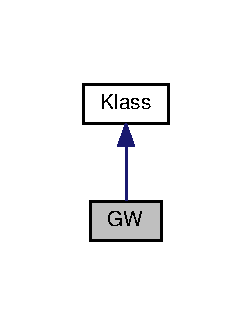
\includegraphics[width=121pt]{class_k_1_1_g_w__inherit__graph}
\end{center}
\end{figure}


Collaboration diagram for GW\+:
\nopagebreak
\begin{figure}[H]
\begin{center}
\leavevmode
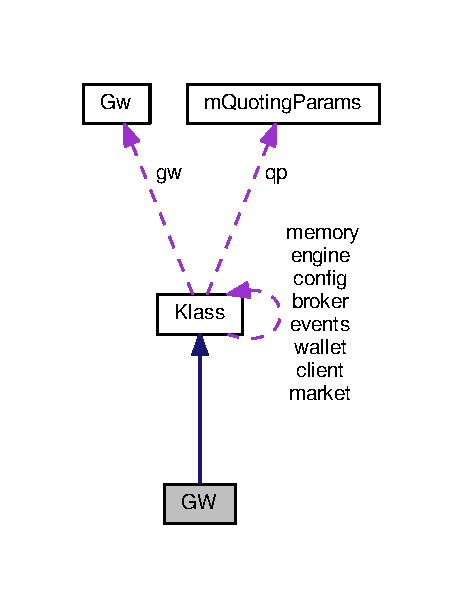
\includegraphics[width=222pt]{class_k_1_1_g_w__coll__graph}
\end{center}
\end{figure}
\subsection*{Protected Member Functions}
\begin{DoxyCompactItemize}
\item 
void \hyperlink{class_k_1_1_g_w_a78f61ac2dd03bcba8e09ca20cd7d68e3}{load} ()
\item 
void \hyperlink{class_k_1_1_g_w_aa9a0f090ee360e2a9f967200d30f4a22}{wait\+Data} ()
\item 
void \hyperlink{class_k_1_1_g_w_ade4c89163dbda531e71c8c75eb2868b4}{wait\+Time} ()
\item 
void \hyperlink{class_k_1_1_g_w_aa3f7b56799f5915cfbc902f6426c2bb2}{wait\+User} ()
\item 
void \hyperlink{class_k_1_1_g_w_a13a43e6d814de94978c515cb084873b1}{run} ()
\end{DoxyCompactItemize}
\subsection*{Additional Inherited Members}


\subsection{Detailed Description}


Definition at line 5 of file gw.\+h.



\subsection{Member Function Documentation}
\index{K\+::\+GW@{K\+::\+GW}!load@{load}}
\index{load@{load}!K\+::\+GW@{K\+::\+GW}}
\subsubsection[{\texorpdfstring{load()}{load()}}]{\setlength{\rightskip}{0pt plus 5cm}void load (
\begin{DoxyParamCaption}
{}
\end{DoxyParamCaption}
)\hspace{0.3cm}{\ttfamily [inline]}, {\ttfamily [protected]}, {\ttfamily [virtual]}}\hypertarget{class_k_1_1_g_w_a78f61ac2dd03bcba8e09ca20cd7d68e3}{}\label{class_k_1_1_g_w_a78f61ac2dd03bcba8e09ca20cd7d68e3}


Reimplemented from \hyperlink{class_k_1_1_klass_a5588964fff1d1025245d134e159b60ee}{Klass}.



Definition at line 18 of file gw.\+h.

\index{K\+::\+GW@{K\+::\+GW}!run@{run}}
\index{run@{run}!K\+::\+GW@{K\+::\+GW}}
\subsubsection[{\texorpdfstring{run()}{run()}}]{\setlength{\rightskip}{0pt plus 5cm}void run (
\begin{DoxyParamCaption}
{}
\end{DoxyParamCaption}
)\hspace{0.3cm}{\ttfamily [inline]}, {\ttfamily [protected]}, {\ttfamily [virtual]}}\hypertarget{class_k_1_1_g_w_a13a43e6d814de94978c515cb084873b1}{}\label{class_k_1_1_g_w_a13a43e6d814de94978c515cb084873b1}


Reimplemented from \hyperlink{class_k_1_1_klass_a72fcb26a14f6beb1c3fbace9ab3e7dbb}{Klass}.



Definition at line 54 of file gw.\+h.

\index{K\+::\+GW@{K\+::\+GW}!wait\+Data@{wait\+Data}}
\index{wait\+Data@{wait\+Data}!K\+::\+GW@{K\+::\+GW}}
\subsubsection[{\texorpdfstring{wait\+Data()}{waitData()}}]{\setlength{\rightskip}{0pt plus 5cm}void wait\+Data (
\begin{DoxyParamCaption}
{}
\end{DoxyParamCaption}
)\hspace{0.3cm}{\ttfamily [inline]}, {\ttfamily [protected]}, {\ttfamily [virtual]}}\hypertarget{class_k_1_1_g_w_aa9a0f090ee360e2a9f967200d30f4a22}{}\label{class_k_1_1_g_w_aa9a0f090ee360e2a9f967200d30f4a22}


Reimplemented from \hyperlink{class_k_1_1_klass_a62a6bf36d7c8bec9dcf7af20c9d21d74}{Klass}.



Definition at line 23 of file gw.\+h.

\index{K\+::\+GW@{K\+::\+GW}!wait\+Time@{wait\+Time}}
\index{wait\+Time@{wait\+Time}!K\+::\+GW@{K\+::\+GW}}
\subsubsection[{\texorpdfstring{wait\+Time()}{waitTime()}}]{\setlength{\rightskip}{0pt plus 5cm}void wait\+Time (
\begin{DoxyParamCaption}
{}
\end{DoxyParamCaption}
)\hspace{0.3cm}{\ttfamily [inline]}, {\ttfamily [protected]}, {\ttfamily [virtual]}}\hypertarget{class_k_1_1_g_w_ade4c89163dbda531e71c8c75eb2868b4}{}\label{class_k_1_1_g_w_ade4c89163dbda531e71c8c75eb2868b4}


Reimplemented from \hyperlink{class_k_1_1_klass_a60afdc2eaa268d8c41a2d6897fbf4fff}{Klass}.



Definition at line 39 of file gw.\+h.

\index{K\+::\+GW@{K\+::\+GW}!wait\+User@{wait\+User}}
\index{wait\+User@{wait\+User}!K\+::\+GW@{K\+::\+GW}}
\subsubsection[{\texorpdfstring{wait\+User()}{waitUser()}}]{\setlength{\rightskip}{0pt plus 5cm}void wait\+User (
\begin{DoxyParamCaption}
{}
\end{DoxyParamCaption}
)\hspace{0.3cm}{\ttfamily [inline]}, {\ttfamily [protected]}, {\ttfamily [virtual]}}\hypertarget{class_k_1_1_g_w_aa3f7b56799f5915cfbc902f6426c2bb2}{}\label{class_k_1_1_g_w_aa3f7b56799f5915cfbc902f6426c2bb2}


Reimplemented from \hyperlink{class_k_1_1_klass_af4f5201bed25a292d8a7f40470d83923}{Klass}.



Definition at line 49 of file gw.\+h.



The documentation for this class was generated from the following file\+:\begin{DoxyCompactItemize}
\item 
\hyperlink{gw_8h}{gw.\+h}\end{DoxyCompactItemize}

\hypertarget{class_k_1_1_gw}{}\section{Gw Class Reference}
\label{class_k_1_1_gw}\index{Gw@{Gw}}


{\ttfamily \#include $<$km.\+h$>$}

\subsection*{Public Member Functions}
\begin{DoxyCompactItemize}
\item 
virtual string \hyperlink{class_k_1_1_gw_aca39965d86b136eea65d98c8797af168}{A} ()=0
\item 
virtual void \hyperlink{class_k_1_1_gw_aaa3aac9b11f8b2d0fd549f88c049e7bb}{send} (\hyperlink{km_8h_a23233b27e494114073abc4d494b05626}{m\+Rand\+Id}, \hyperlink{km_8h_a23233b27e494114073abc4d494b05626}{m\+Rand\+Id}, \hyperlink{km_8h_a23233b27e494114073abc4d494b05626}{m\+Rand\+Id}, \hyperlink{namespace_k_a0b7d0fa0ffc9f87da1d6499cbcee7e94}{m\+Side}, string, string, \hyperlink{namespace_k_a131435180aff10fab1bf3da09af62b0d}{m\+Order\+Type}, \hyperlink{namespace_k_a290fccb3fc7d447fdbb93a61f6dfba44}{m\+Time\+In\+Force}, bool, \hyperlink{km_8h_ad02a70cba4c52ba2013e5e32ceaeac1c}{m\+Clock})=0
\item 
virtual void \hyperlink{class_k_1_1_gw_a20fa6fadc0acc192eec1f324742135ca}{cancel} (\hyperlink{km_8h_a23233b27e494114073abc4d494b05626}{m\+Rand\+Id}, \hyperlink{km_8h_a23233b27e494114073abc4d494b05626}{m\+Rand\+Id}, \hyperlink{namespace_k_a0b7d0fa0ffc9f87da1d6499cbcee7e94}{m\+Side}, \hyperlink{km_8h_ad02a70cba4c52ba2013e5e32ceaeac1c}{m\+Clock})=0
\item 
virtual void \hyperlink{class_k_1_1_gw_af6ee7eacbde6b379b68d954e44f6e549}{close} ()=0
\item 
bool \hyperlink{class_k_1_1_gw_ac4c94b7be7f6b0bfe7e42e31d965923c}{wait\+For\+Data} ()
\item 
virtual bool \hyperlink{class_k_1_1_gw_ad1293382b9b42a2fb3e1119078f97ca4}{async\+\_\+levels} ()
\item 
virtual bool \hyperlink{class_k_1_1_gw_aadf97204c27f5ef667c159182fac5e26}{async\+\_\+trades} ()
\item 
virtual bool \hyperlink{class_k_1_1_gw_aae17c049f2524a26e52ba61080b06fda}{async\+\_\+orders} ()
\item 
virtual vector$<$ \hyperlink{struct_k_1_1m_order}{m\+Order} $>$ \hyperlink{class_k_1_1_gw_aae707e552babec2a6f663f1c79745206}{sync\+\_\+cancel\+All} ()=0
\end{DoxyCompactItemize}
\subsection*{Static Public Member Functions}
\begin{DoxyCompactItemize}
\item 
static \hyperlink{class_k_1_1_gw}{Gw} $\ast$ \hyperlink{class_k_1_1_gw_a282f7bac1cca98304b43013414a068af}{config} (\hyperlink{km_8h_a0299927fb26276a1e0f4c2b4dedb698e}{m\+Coin\+Id}, \hyperlink{km_8h_a0299927fb26276a1e0f4c2b4dedb698e}{m\+Coin\+Id}, string, int, string, string, string, string, string, string, int, int, int)
\end{DoxyCompactItemize}
\subsection*{Data Fields}
\begin{DoxyCompactItemize}
\item 
u\+W\+S\+::\+Hub $\ast$ \hyperlink{class_k_1_1_gw_a33b00844a7c4d5c91a4696d71e02bafd}{hub} = nullptr
\item 
u\+W\+S\+::\+Group$<$ u\+W\+S\+::\+C\+L\+I\+E\+NT $>$ $\ast$ \hyperlink{class_k_1_1_gw_a57ae195e4262e03d47cad44c3a0b09f1}{gw\+Group} = nullptr
\item 
function$<$ void(string)$>$ \hyperlink{class_k_1_1_gw_a45c045408bc39a1e18f99b18505a0859}{log}
\item 
function$<$ void(string)$>$ \hyperlink{class_k_1_1_gw_acedf7f89824adaf984f2ff0cbb29961a}{reconnect}
\item 
function$<$ void(\hyperlink{struct_k_1_1m_order}{m\+Order})$>$ \hyperlink{class_k_1_1_gw_adf1e832cf66132207c5b97edb28437bf}{ev\+Data\+Order}
\item 
function$<$ void(\hyperlink{struct_k_1_1m_trade}{m\+Trade})$>$ \hyperlink{class_k_1_1_gw_a6cdc51ebb4004f0a69afafb623d9d7e0}{ev\+Data\+Trade}
\item 
function$<$ void(\hyperlink{struct_k_1_1m_levels}{m\+Levels})$>$ \hyperlink{class_k_1_1_gw_a2d20ec3398210965d042521449f1d890}{ev\+Data\+Levels}
\item 
function$<$ void(\hyperlink{struct_k_1_1m_wallets}{m\+Wallets})$>$ \hyperlink{class_k_1_1_gw_ae539d2c47a0e797655fea7dcc8666408}{ev\+Data\+Wallet}
\item 
function$<$ void(\hyperlink{namespace_k_a3da250819294c55d5728586148bfa19e}{m\+Connectivity})$>$ \hyperlink{class_k_1_1_gw_a2a25d79475922457931affe36df2223f}{ev\+Connect\+Order}
\item 
function$<$ void(\hyperlink{namespace_k_a3da250819294c55d5728586148bfa19e}{m\+Connectivity})$>$ \hyperlink{class_k_1_1_gw_a9df19921d4fe9fc1aab360b9605fd451}{ev\+Connect\+Market}
\item 
\hyperlink{namespace_k_a7ab53d1849aa2c29d90459c21afa8c17}{m\+Exchange} \hyperlink{class_k_1_1_gw_ab20a118abdc21d41ee2c9a5ae01212db}{exchange} = (\hyperlink{namespace_k_a7ab53d1849aa2c29d90459c21afa8c17}{m\+Exchange})0
\item 
int \hyperlink{class_k_1_1_gw_aad880fc4455c253781e8968f2239d56f}{version} = 0
\item 
int \hyperlink{class_k_1_1_gw_a8811afa719f86cb7ddde8770eb580fdc}{max\+Level} = 0
\item 
int \hyperlink{class_k_1_1_gw_ac3e1795766a80ec63b157951b4b9a7d4}{debug} = 0
\item 
int \hyperlink{class_k_1_1_gw_a8eb87e9b99a80ee81ff9114f6241b8d4}{chamber} = 0
\item 
\hyperlink{km_8h_a392f9b7f384aa3539bbb890b059f5b8c}{m\+Price} \hyperlink{class_k_1_1_gw_a86d946748d0cea5c3fb3ab8ae81cf23a}{min\+Tick} = 0
\item 
\hyperlink{km_8h_ad4d00888c55a47a8a40ed8020d176086}{m\+Amount} \hyperlink{class_k_1_1_gw_a379233bfc2ba83fd276d17dbe2e37009}{make\+Fee} = 0
\item 
\hyperlink{km_8h_ad4d00888c55a47a8a40ed8020d176086}{m\+Amount} \hyperlink{class_k_1_1_gw_a1a5ea3c2a5f11d2100866df8ae3b32fe}{take\+Fee} = 0
\item 
\hyperlink{km_8h_ad4d00888c55a47a8a40ed8020d176086}{m\+Amount} \hyperlink{class_k_1_1_gw_a9814db79743d44d6def92893a4b43b84}{min\+Size} = 0
\item 
\hyperlink{km_8h_a0299927fb26276a1e0f4c2b4dedb698e}{m\+Coin\+Id} \hyperlink{class_k_1_1_gw_a88838a75375332fd734e38ba4d7d870c}{base} = \char`\"{}\char`\"{}
\item 
\hyperlink{km_8h_a0299927fb26276a1e0f4c2b4dedb698e}{m\+Coin\+Id} \hyperlink{class_k_1_1_gw_abb05d77de0b838cdc580fe5759070aad}{quote} = \char`\"{}\char`\"{}
\item 
string \hyperlink{class_k_1_1_gw_a8ccf841cb59e451791bcb2e1ac4f1edc}{name} = \char`\"{}\char`\"{}
\item 
string \hyperlink{class_k_1_1_gw_aa0183fad0a4c5c8a30c8fdc7b81a1279}{symbol} = \char`\"{}\char`\"{}
\item 
string \hyperlink{class_k_1_1_gw_a0372bca04753136de90e3cd45085dc45}{apikey} = \char`\"{}\char`\"{}
\item 
string \hyperlink{class_k_1_1_gw_ae27f9f88345b7cc8388e912993d34b69}{secret} = \char`\"{}\char`\"{}
\item 
string \hyperlink{class_k_1_1_gw_ae315dc7095b2ab26df1efb90a58f6345}{user} = \char`\"{}\char`\"{}
\item 
string \hyperlink{class_k_1_1_gw_a2805cc9b0dd93ef48a266ab19ebfd7c1}{pass} = \char`\"{}\char`\"{}
\item 
string \hyperlink{class_k_1_1_gw_a9a2c0c2e6f162d2d9155ba02e513d978}{ws} = \char`\"{}\char`\"{}
\item 
string \hyperlink{class_k_1_1_gw_a316cb611c8cb905b1c208e7c4f38bb4e}{http} = \char`\"{}\char`\"{}
\item 
bool \hyperlink{class_k_1_1_gw_a8bdead4768d804f7a81639dee1e456f2}{force\+Update} = false
\item 
\hyperlink{km_8h_a23233b27e494114073abc4d494b05626}{m\+Rand\+Id}($\ast$ \hyperlink{class_k_1_1_gw_ae3eceb5a8284748fe41ebb9e201cffbf}{rand\+Id} )()=0
\item 
function$<$ bool()$>$ \hyperlink{class_k_1_1_gw_a2381015e1bae39f4cfd8e158bec8161a}{wallet} = \mbox{[}\&\mbox{]}() \{ return !(\hyperlink{class_k_1_1_gw_a69bd12a2ef6f58b5a44c15b3801c2ef2}{async\+\_\+wallet}() or !\hyperlink{class_k_1_1_gw_af6748577cac6d6171379036bcd243228}{ask\+For}(\hyperlink{class_k_1_1_gw_af1978cbd97d41a4197e481dc8fdfa5eb}{reply\+Wallets}, \mbox{[}\&\mbox{]}() \{ return \hyperlink{class_k_1_1_gw_a45b0afcbe68c422db35af9b503831be5}{sync\+\_\+wallet}(); \})); \}
\item 
function$<$ bool()$>$ \hyperlink{class_k_1_1_gw_a167ae09c2d39a1aee89c080bf58c7fb3}{levels} = \mbox{[}\&\mbox{]}() \{ return \hyperlink{class_k_1_1_gw_af6748577cac6d6171379036bcd243228}{ask\+For}(\hyperlink{class_k_1_1_gw_a37ee3b756d9b6633e81ff28125314fab}{reply\+Levels}, \mbox{[}\&\mbox{]}() \{ return \hyperlink{class_k_1_1_gw_ac20ee1cedc4725a39815f28d36470fa1}{sync\+\_\+levels}(); \}); \}
\item 
function$<$ bool()$>$ \hyperlink{class_k_1_1_gw_a2e04da03fb9d2f9179864a70244aedb9}{trades} = \mbox{[}\&\mbox{]}() \{ return \hyperlink{class_k_1_1_gw_af6748577cac6d6171379036bcd243228}{ask\+For}(\hyperlink{class_k_1_1_gw_a3648d850c8042fbb808b77b0ebec8087}{reply\+Trades}, \mbox{[}\&\mbox{]}() \{ return \hyperlink{class_k_1_1_gw_a41fa6e2cd171072202fa1e44fbd780c5}{sync\+\_\+trades}(); \}); \}
\item 
function$<$ bool()$>$ \hyperlink{class_k_1_1_gw_ab56786d35b5f78826316091dfb92b300}{orders} = \mbox{[}\&\mbox{]}() \{ return \hyperlink{class_k_1_1_gw_af6748577cac6d6171379036bcd243228}{ask\+For}(\hyperlink{class_k_1_1_gw_ab6cf63a19336c99e031b44359e68814f}{reply\+Orders}, \mbox{[}\&\mbox{]}() \{ return \hyperlink{class_k_1_1_gw_a96bb7b05334000c911a75894711853c4}{sync\+\_\+orders}(); \}); \}
\item 
function$<$ bool()$>$ \hyperlink{class_k_1_1_gw_a14d117d8e7284953667f53db89f1700c}{cancel\+All} = \mbox{[}\&\mbox{]}() \{ return \hyperlink{class_k_1_1_gw_af6748577cac6d6171379036bcd243228}{ask\+For}(\hyperlink{class_k_1_1_gw_a02a0f0472ebae5925916a1d6661f8375}{reply\+Cancel\+All}, \mbox{[}\&\mbox{]}() \{ return \hyperlink{class_k_1_1_gw_aae707e552babec2a6f663f1c79745206}{sync\+\_\+cancel\+All}(); \}); \}
\end{DoxyCompactItemize}
\subsection*{Protected Member Functions}
\begin{DoxyCompactItemize}
\item 
virtual bool \hyperlink{class_k_1_1_gw_a69bd12a2ef6f58b5a44c15b3801c2ef2}{async\+\_\+wallet} ()
\item 
virtual vector$<$ \hyperlink{struct_k_1_1m_wallets}{m\+Wallets} $>$ \hyperlink{class_k_1_1_gw_a45b0afcbe68c422db35af9b503831be5}{sync\+\_\+wallet} ()
\item 
virtual vector$<$ \hyperlink{struct_k_1_1m_levels}{m\+Levels} $>$ \hyperlink{class_k_1_1_gw_ac20ee1cedc4725a39815f28d36470fa1}{sync\+\_\+levels} ()
\item 
virtual vector$<$ \hyperlink{struct_k_1_1m_trade}{m\+Trade} $>$ \hyperlink{class_k_1_1_gw_a41fa6e2cd171072202fa1e44fbd780c5}{sync\+\_\+trades} ()
\item 
virtual vector$<$ \hyperlink{struct_k_1_1m_order}{m\+Order} $>$ \hyperlink{class_k_1_1_gw_a96bb7b05334000c911a75894711853c4}{sync\+\_\+orders} ()
\item 
{\footnotesize template$<$typename m\+Data , typename sync $>$ }\\bool \hyperlink{class_k_1_1_gw_af6748577cac6d6171379036bcd243228}{ask\+For} (future$<$ vector$<$ m\+Data $>$$>$ \&reply, sync fn)
\item 
{\footnotesize template$<$typename m\+Data $>$ }\\unsigned int \hyperlink{class_k_1_1_gw_a96ddc8b55247c87b0ecbbba76c71b01a}{wait\+For} (future$<$ vector$<$ m\+Data $>$$>$ \&reply, function$<$ void(m\+Data)$>$ \&fn)
\end{DoxyCompactItemize}
\subsection*{Protected Attributes}
\begin{DoxyCompactItemize}
\item 
future$<$ vector$<$ \hyperlink{struct_k_1_1m_wallets}{m\+Wallets} $>$ $>$ \hyperlink{class_k_1_1_gw_af1978cbd97d41a4197e481dc8fdfa5eb}{reply\+Wallets}
\item 
future$<$ vector$<$ \hyperlink{struct_k_1_1m_levels}{m\+Levels} $>$ $>$ \hyperlink{class_k_1_1_gw_a37ee3b756d9b6633e81ff28125314fab}{reply\+Levels}
\item 
future$<$ vector$<$ \hyperlink{struct_k_1_1m_trade}{m\+Trade} $>$ $>$ \hyperlink{class_k_1_1_gw_a3648d850c8042fbb808b77b0ebec8087}{reply\+Trades}
\item 
future$<$ vector$<$ \hyperlink{struct_k_1_1m_order}{m\+Order} $>$ $>$ \hyperlink{class_k_1_1_gw_ab6cf63a19336c99e031b44359e68814f}{reply\+Orders}
\item 
future$<$ vector$<$ \hyperlink{struct_k_1_1m_order}{m\+Order} $>$ $>$ \hyperlink{class_k_1_1_gw_a02a0f0472ebae5925916a1d6661f8375}{reply\+Cancel\+All}
\end{DoxyCompactItemize}


\subsection{Detailed Description}


Definition at line 655 of file km.\+h.



\subsection{Member Function Documentation}
\index{K\+::\+Gw@{K\+::\+Gw}!A@{A}}
\index{A@{A}!K\+::\+Gw@{K\+::\+Gw}}
\subsubsection[{\texorpdfstring{A()=0}{A()=0}}]{\setlength{\rightskip}{0pt plus 5cm}virtual string A (
\begin{DoxyParamCaption}
{}
\end{DoxyParamCaption}
)\hspace{0.3cm}{\ttfamily [pure virtual]}}\hypertarget{class_k_1_1_gw_aca39965d86b136eea65d98c8797af168}{}\label{class_k_1_1_gw_aca39965d86b136eea65d98c8797af168}
\index{K\+::\+Gw@{K\+::\+Gw}!ask\+For@{ask\+For}}
\index{ask\+For@{ask\+For}!K\+::\+Gw@{K\+::\+Gw}}
\subsubsection[{\texorpdfstring{ask\+For(future$<$ vector$<$ m\+Data $>$$>$ \&reply, sync fn)}{askFor(future< vector< mData >> &reply, sync fn)}}]{\setlength{\rightskip}{0pt plus 5cm}bool ask\+For (
\begin{DoxyParamCaption}
\item[{future$<$ vector$<$ m\+Data $>$$>$ \&}]{reply, }
\item[{sync}]{fn}
\end{DoxyParamCaption}
)\hspace{0.3cm}{\ttfamily [inline]}, {\ttfamily [protected]}}\hypertarget{class_k_1_1_gw_af6748577cac6d6171379036bcd243228}{}\label{class_k_1_1_gw_af6748577cac6d6171379036bcd243228}


Definition at line 712 of file km.\+h.

\index{K\+::\+Gw@{K\+::\+Gw}!async\+\_\+levels@{async\+\_\+levels}}
\index{async\+\_\+levels@{async\+\_\+levels}!K\+::\+Gw@{K\+::\+Gw}}
\subsubsection[{\texorpdfstring{async\+\_\+levels()}{async_levels()}}]{\setlength{\rightskip}{0pt plus 5cm}virtual bool async\+\_\+levels (
\begin{DoxyParamCaption}
{}
\end{DoxyParamCaption}
)\hspace{0.3cm}{\ttfamily [inline]}, {\ttfamily [virtual]}}\hypertarget{class_k_1_1_gw_ad1293382b9b42a2fb3e1119078f97ca4}{}\label{class_k_1_1_gw_ad1293382b9b42a2fb3e1119078f97ca4}


Definition at line 697 of file km.\+h.

\index{K\+::\+Gw@{K\+::\+Gw}!async\+\_\+orders@{async\+\_\+orders}}
\index{async\+\_\+orders@{async\+\_\+orders}!K\+::\+Gw@{K\+::\+Gw}}
\subsubsection[{\texorpdfstring{async\+\_\+orders()}{async_orders()}}]{\setlength{\rightskip}{0pt plus 5cm}virtual bool async\+\_\+orders (
\begin{DoxyParamCaption}
{}
\end{DoxyParamCaption}
)\hspace{0.3cm}{\ttfamily [inline]}, {\ttfamily [virtual]}}\hypertarget{class_k_1_1_gw_aae17c049f2524a26e52ba61080b06fda}{}\label{class_k_1_1_gw_aae17c049f2524a26e52ba61080b06fda}


Definition at line 699 of file km.\+h.

\index{K\+::\+Gw@{K\+::\+Gw}!async\+\_\+trades@{async\+\_\+trades}}
\index{async\+\_\+trades@{async\+\_\+trades}!K\+::\+Gw@{K\+::\+Gw}}
\subsubsection[{\texorpdfstring{async\+\_\+trades()}{async_trades()}}]{\setlength{\rightskip}{0pt plus 5cm}virtual bool async\+\_\+trades (
\begin{DoxyParamCaption}
{}
\end{DoxyParamCaption}
)\hspace{0.3cm}{\ttfamily [inline]}, {\ttfamily [virtual]}}\hypertarget{class_k_1_1_gw_aadf97204c27f5ef667c159182fac5e26}{}\label{class_k_1_1_gw_aadf97204c27f5ef667c159182fac5e26}


Definition at line 698 of file km.\+h.

\index{K\+::\+Gw@{K\+::\+Gw}!async\+\_\+wallet@{async\+\_\+wallet}}
\index{async\+\_\+wallet@{async\+\_\+wallet}!K\+::\+Gw@{K\+::\+Gw}}
\subsubsection[{\texorpdfstring{async\+\_\+wallet()}{async_wallet()}}]{\setlength{\rightskip}{0pt plus 5cm}virtual bool async\+\_\+wallet (
\begin{DoxyParamCaption}
{}
\end{DoxyParamCaption}
)\hspace{0.3cm}{\ttfamily [inline]}, {\ttfamily [protected]}, {\ttfamily [virtual]}}\hypertarget{class_k_1_1_gw_a69bd12a2ef6f58b5a44c15b3801c2ef2}{}\label{class_k_1_1_gw_a69bd12a2ef6f58b5a44c15b3801c2ef2}


Definition at line 702 of file km.\+h.

\index{K\+::\+Gw@{K\+::\+Gw}!cancel@{cancel}}
\index{cancel@{cancel}!K\+::\+Gw@{K\+::\+Gw}}
\subsubsection[{\texorpdfstring{cancel(m\+Rand\+Id, m\+Rand\+Id, m\+Side, m\+Clock)=0}{cancel(mRandId, mRandId, mSide, mClock)=0}}]{\setlength{\rightskip}{0pt plus 5cm}virtual void cancel (
\begin{DoxyParamCaption}
\item[{{\bf m\+Rand\+Id}}]{, }
\item[{{\bf m\+Rand\+Id}}]{, }
\item[{{\bf m\+Side}}]{, }
\item[{{\bf m\+Clock}}]{}
\end{DoxyParamCaption}
)\hspace{0.3cm}{\ttfamily [pure virtual]}}\hypertarget{class_k_1_1_gw_a20fa6fadc0acc192eec1f324742135ca}{}\label{class_k_1_1_gw_a20fa6fadc0acc192eec1f324742135ca}
\index{K\+::\+Gw@{K\+::\+Gw}!close@{close}}
\index{close@{close}!K\+::\+Gw@{K\+::\+Gw}}
\subsubsection[{\texorpdfstring{close()=0}{close()=0}}]{\setlength{\rightskip}{0pt plus 5cm}virtual void close (
\begin{DoxyParamCaption}
{}
\end{DoxyParamCaption}
)\hspace{0.3cm}{\ttfamily [pure virtual]}}\hypertarget{class_k_1_1_gw_af6ee7eacbde6b379b68d954e44f6e549}{}\label{class_k_1_1_gw_af6ee7eacbde6b379b68d954e44f6e549}
\index{K\+::\+Gw@{K\+::\+Gw}!config@{config}}
\index{config@{config}!K\+::\+Gw@{K\+::\+Gw}}
\subsubsection[{\texorpdfstring{config(m\+Coin\+Id, m\+Coin\+Id, string, int, string, string, string, string, string, string, int, int, int)}{config(mCoinId, mCoinId, string, int, string, string, string, string, string, string, int, int, int)}}]{\setlength{\rightskip}{0pt plus 5cm}static {\bf Gw}$\ast$ config (
\begin{DoxyParamCaption}
\item[{{\bf m\+Coin\+Id}}]{, }
\item[{{\bf m\+Coin\+Id}}]{, }
\item[{string}]{, }
\item[{int}]{, }
\item[{string}]{, }
\item[{string}]{, }
\item[{string}]{, }
\item[{string}]{, }
\item[{string}]{, }
\item[{string}]{, }
\item[{int}]{, }
\item[{int}]{, }
\item[{int}]{}
\end{DoxyParamCaption}
)\hspace{0.3cm}{\ttfamily [static]}}\hypertarget{class_k_1_1_gw_a282f7bac1cca98304b43013414a068af}{}\label{class_k_1_1_gw_a282f7bac1cca98304b43013414a068af}
\index{K\+::\+Gw@{K\+::\+Gw}!send@{send}}
\index{send@{send}!K\+::\+Gw@{K\+::\+Gw}}
\subsubsection[{\texorpdfstring{send(m\+Rand\+Id, m\+Rand\+Id, m\+Rand\+Id, m\+Side, string, string, m\+Order\+Type, m\+Time\+In\+Force, bool, m\+Clock)=0}{send(mRandId, mRandId, mRandId, mSide, string, string, mOrderType, mTimeInForce, bool, mClock)=0}}]{\setlength{\rightskip}{0pt plus 5cm}virtual void send (
\begin{DoxyParamCaption}
\item[{{\bf m\+Rand\+Id}}]{, }
\item[{{\bf m\+Rand\+Id}}]{, }
\item[{{\bf m\+Rand\+Id}}]{, }
\item[{{\bf m\+Side}}]{, }
\item[{string}]{, }
\item[{string}]{, }
\item[{{\bf m\+Order\+Type}}]{, }
\item[{{\bf m\+Time\+In\+Force}}]{, }
\item[{bool}]{, }
\item[{{\bf m\+Clock}}]{}
\end{DoxyParamCaption}
)\hspace{0.3cm}{\ttfamily [pure virtual]}}\hypertarget{class_k_1_1_gw_aaa3aac9b11f8b2d0fd549f88c049e7bb}{}\label{class_k_1_1_gw_aaa3aac9b11f8b2d0fd549f88c049e7bb}
\index{K\+::\+Gw@{K\+::\+Gw}!sync\+\_\+cancel\+All@{sync\+\_\+cancel\+All}}
\index{sync\+\_\+cancel\+All@{sync\+\_\+cancel\+All}!K\+::\+Gw@{K\+::\+Gw}}
\subsubsection[{\texorpdfstring{sync\+\_\+cancel\+All()=0}{sync_cancelAll()=0}}]{\setlength{\rightskip}{0pt plus 5cm}virtual vector$<${\bf m\+Order}$>$ sync\+\_\+cancel\+All (
\begin{DoxyParamCaption}
{}
\end{DoxyParamCaption}
)\hspace{0.3cm}{\ttfamily [pure virtual]}}\hypertarget{class_k_1_1_gw_aae707e552babec2a6f663f1c79745206}{}\label{class_k_1_1_gw_aae707e552babec2a6f663f1c79745206}
\index{K\+::\+Gw@{K\+::\+Gw}!sync\+\_\+levels@{sync\+\_\+levels}}
\index{sync\+\_\+levels@{sync\+\_\+levels}!K\+::\+Gw@{K\+::\+Gw}}
\subsubsection[{\texorpdfstring{sync\+\_\+levels()}{sync_levels()}}]{\setlength{\rightskip}{0pt plus 5cm}virtual vector$<${\bf m\+Levels}$>$ sync\+\_\+levels (
\begin{DoxyParamCaption}
{}
\end{DoxyParamCaption}
)\hspace{0.3cm}{\ttfamily [inline]}, {\ttfamily [protected]}, {\ttfamily [virtual]}}\hypertarget{class_k_1_1_gw_ac20ee1cedc4725a39815f28d36470fa1}{}\label{class_k_1_1_gw_ac20ee1cedc4725a39815f28d36470fa1}


Definition at line 704 of file km.\+h.

\index{K\+::\+Gw@{K\+::\+Gw}!sync\+\_\+orders@{sync\+\_\+orders}}
\index{sync\+\_\+orders@{sync\+\_\+orders}!K\+::\+Gw@{K\+::\+Gw}}
\subsubsection[{\texorpdfstring{sync\+\_\+orders()}{sync_orders()}}]{\setlength{\rightskip}{0pt plus 5cm}virtual vector$<${\bf m\+Order}$>$ sync\+\_\+orders (
\begin{DoxyParamCaption}
{}
\end{DoxyParamCaption}
)\hspace{0.3cm}{\ttfamily [inline]}, {\ttfamily [protected]}, {\ttfamily [virtual]}}\hypertarget{class_k_1_1_gw_a96bb7b05334000c911a75894711853c4}{}\label{class_k_1_1_gw_a96bb7b05334000c911a75894711853c4}


Definition at line 706 of file km.\+h.

\index{K\+::\+Gw@{K\+::\+Gw}!sync\+\_\+trades@{sync\+\_\+trades}}
\index{sync\+\_\+trades@{sync\+\_\+trades}!K\+::\+Gw@{K\+::\+Gw}}
\subsubsection[{\texorpdfstring{sync\+\_\+trades()}{sync_trades()}}]{\setlength{\rightskip}{0pt plus 5cm}virtual vector$<${\bf m\+Trade}$>$ sync\+\_\+trades (
\begin{DoxyParamCaption}
{}
\end{DoxyParamCaption}
)\hspace{0.3cm}{\ttfamily [inline]}, {\ttfamily [protected]}, {\ttfamily [virtual]}}\hypertarget{class_k_1_1_gw_a41fa6e2cd171072202fa1e44fbd780c5}{}\label{class_k_1_1_gw_a41fa6e2cd171072202fa1e44fbd780c5}


Definition at line 705 of file km.\+h.

\index{K\+::\+Gw@{K\+::\+Gw}!sync\+\_\+wallet@{sync\+\_\+wallet}}
\index{sync\+\_\+wallet@{sync\+\_\+wallet}!K\+::\+Gw@{K\+::\+Gw}}
\subsubsection[{\texorpdfstring{sync\+\_\+wallet()}{sync_wallet()}}]{\setlength{\rightskip}{0pt plus 5cm}virtual vector$<${\bf m\+Wallets}$>$ sync\+\_\+wallet (
\begin{DoxyParamCaption}
{}
\end{DoxyParamCaption}
)\hspace{0.3cm}{\ttfamily [inline]}, {\ttfamily [protected]}, {\ttfamily [virtual]}}\hypertarget{class_k_1_1_gw_a45b0afcbe68c422db35af9b503831be5}{}\label{class_k_1_1_gw_a45b0afcbe68c422db35af9b503831be5}


Definition at line 703 of file km.\+h.

\index{K\+::\+Gw@{K\+::\+Gw}!wait\+For@{wait\+For}}
\index{wait\+For@{wait\+For}!K\+::\+Gw@{K\+::\+Gw}}
\subsubsection[{\texorpdfstring{wait\+For(future$<$ vector$<$ m\+Data $>$$>$ \&reply, function$<$ void(m\+Data)$>$ \&fn)}{waitFor(future< vector< mData >> &reply, function< void(mData)> &fn)}}]{\setlength{\rightskip}{0pt plus 5cm}unsigned int wait\+For (
\begin{DoxyParamCaption}
\item[{future$<$ vector$<$ m\+Data $>$$>$ \&}]{reply, }
\item[{function$<$ void(m\+Data)$>$ \&}]{fn}
\end{DoxyParamCaption}
)\hspace{0.3cm}{\ttfamily [inline]}, {\ttfamily [protected]}}\hypertarget{class_k_1_1_gw_a96ddc8b55247c87b0ecbbba76c71b01a}{}\label{class_k_1_1_gw_a96ddc8b55247c87b0ecbbba76c71b01a}


Definition at line 720 of file km.\+h.

\index{K\+::\+Gw@{K\+::\+Gw}!wait\+For\+Data@{wait\+For\+Data}}
\index{wait\+For\+Data@{wait\+For\+Data}!K\+::\+Gw@{K\+::\+Gw}}
\subsubsection[{\texorpdfstring{wait\+For\+Data()}{waitForData()}}]{\setlength{\rightskip}{0pt plus 5cm}bool wait\+For\+Data (
\begin{DoxyParamCaption}
{}
\end{DoxyParamCaption}
)\hspace{0.3cm}{\ttfamily [inline]}}\hypertarget{class_k_1_1_gw_ac4c94b7be7f6b0bfe7e42e31d965923c}{}\label{class_k_1_1_gw_ac4c94b7be7f6b0bfe7e42e31d965923c}


Definition at line 685 of file km.\+h.



\subsection{Field Documentation}
\index{K\+::\+Gw@{K\+::\+Gw}!apikey@{apikey}}
\index{apikey@{apikey}!K\+::\+Gw@{K\+::\+Gw}}
\subsubsection[{\texorpdfstring{apikey}{apikey}}]{\setlength{\rightskip}{0pt plus 5cm}string apikey = \char`\"{}\char`\"{}}\hypertarget{class_k_1_1_gw_a0372bca04753136de90e3cd45085dc45}{}\label{class_k_1_1_gw_a0372bca04753136de90e3cd45085dc45}


Definition at line 677 of file km.\+h.

\index{K\+::\+Gw@{K\+::\+Gw}!base@{base}}
\index{base@{base}!K\+::\+Gw@{K\+::\+Gw}}
\subsubsection[{\texorpdfstring{base}{base}}]{\setlength{\rightskip}{0pt plus 5cm}{\bf m\+Coin\+Id} base = \char`\"{}\char`\"{}}\hypertarget{class_k_1_1_gw_a88838a75375332fd734e38ba4d7d870c}{}\label{class_k_1_1_gw_a88838a75375332fd734e38ba4d7d870c}


Definition at line 675 of file km.\+h.

\index{K\+::\+Gw@{K\+::\+Gw}!cancel\+All@{cancel\+All}}
\index{cancel\+All@{cancel\+All}!K\+::\+Gw@{K\+::\+Gw}}
\subsubsection[{\texorpdfstring{cancel\+All}{cancelAll}}]{\setlength{\rightskip}{0pt plus 5cm}function$<$bool()$>$ cancel\+All = \mbox{[}\&\mbox{]}() \{ return {\bf ask\+For}({\bf reply\+Cancel\+All}, \mbox{[}\&\mbox{]}() \{ return {\bf sync\+\_\+cancel\+All}(); \}); \}}\hypertarget{class_k_1_1_gw_a14d117d8e7284953667f53db89f1700c}{}\label{class_k_1_1_gw_a14d117d8e7284953667f53db89f1700c}


Definition at line 696 of file km.\+h.

\index{K\+::\+Gw@{K\+::\+Gw}!chamber@{chamber}}
\index{chamber@{chamber}!K\+::\+Gw@{K\+::\+Gw}}
\subsubsection[{\texorpdfstring{chamber}{chamber}}]{\setlength{\rightskip}{0pt plus 5cm}int chamber = 0}\hypertarget{class_k_1_1_gw_a8eb87e9b99a80ee81ff9114f6241b8d4}{}\label{class_k_1_1_gw_a8eb87e9b99a80ee81ff9114f6241b8d4}


Definition at line 671 of file km.\+h.

\index{K\+::\+Gw@{K\+::\+Gw}!debug@{debug}}
\index{debug@{debug}!K\+::\+Gw@{K\+::\+Gw}}
\subsubsection[{\texorpdfstring{debug}{debug}}]{\setlength{\rightskip}{0pt plus 5cm}int debug = 0}\hypertarget{class_k_1_1_gw_ac3e1795766a80ec63b157951b4b9a7d4}{}\label{class_k_1_1_gw_ac3e1795766a80ec63b157951b4b9a7d4}


Definition at line 671 of file km.\+h.

\index{K\+::\+Gw@{K\+::\+Gw}!ev\+Connect\+Market@{ev\+Connect\+Market}}
\index{ev\+Connect\+Market@{ev\+Connect\+Market}!K\+::\+Gw@{K\+::\+Gw}}
\subsubsection[{\texorpdfstring{ev\+Connect\+Market}{evConnectMarket}}]{\setlength{\rightskip}{0pt plus 5cm}function$<$void({\bf m\+Connectivity})$>$ ev\+Connect\+Market}\hypertarget{class_k_1_1_gw_a9df19921d4fe9fc1aab360b9605fd451}{}\label{class_k_1_1_gw_a9df19921d4fe9fc1aab360b9605fd451}


Definition at line 667 of file km.\+h.

\index{K\+::\+Gw@{K\+::\+Gw}!ev\+Connect\+Order@{ev\+Connect\+Order}}
\index{ev\+Connect\+Order@{ev\+Connect\+Order}!K\+::\+Gw@{K\+::\+Gw}}
\subsubsection[{\texorpdfstring{ev\+Connect\+Order}{evConnectOrder}}]{\setlength{\rightskip}{0pt plus 5cm}function$<$void({\bf m\+Connectivity})$>$ ev\+Connect\+Order}\hypertarget{class_k_1_1_gw_a2a25d79475922457931affe36df2223f}{}\label{class_k_1_1_gw_a2a25d79475922457931affe36df2223f}


Definition at line 667 of file km.\+h.

\index{K\+::\+Gw@{K\+::\+Gw}!ev\+Data\+Levels@{ev\+Data\+Levels}}
\index{ev\+Data\+Levels@{ev\+Data\+Levels}!K\+::\+Gw@{K\+::\+Gw}}
\subsubsection[{\texorpdfstring{ev\+Data\+Levels}{evDataLevels}}]{\setlength{\rightskip}{0pt plus 5cm}function$<$void({\bf m\+Levels})$>$ ev\+Data\+Levels}\hypertarget{class_k_1_1_gw_a2d20ec3398210965d042521449f1d890}{}\label{class_k_1_1_gw_a2d20ec3398210965d042521449f1d890}


Definition at line 665 of file km.\+h.

\index{K\+::\+Gw@{K\+::\+Gw}!ev\+Data\+Order@{ev\+Data\+Order}}
\index{ev\+Data\+Order@{ev\+Data\+Order}!K\+::\+Gw@{K\+::\+Gw}}
\subsubsection[{\texorpdfstring{ev\+Data\+Order}{evDataOrder}}]{\setlength{\rightskip}{0pt plus 5cm}function$<$void({\bf m\+Order})$>$ ev\+Data\+Order}\hypertarget{class_k_1_1_gw_adf1e832cf66132207c5b97edb28437bf}{}\label{class_k_1_1_gw_adf1e832cf66132207c5b97edb28437bf}


Definition at line 663 of file km.\+h.

\index{K\+::\+Gw@{K\+::\+Gw}!ev\+Data\+Trade@{ev\+Data\+Trade}}
\index{ev\+Data\+Trade@{ev\+Data\+Trade}!K\+::\+Gw@{K\+::\+Gw}}
\subsubsection[{\texorpdfstring{ev\+Data\+Trade}{evDataTrade}}]{\setlength{\rightskip}{0pt plus 5cm}function$<$void({\bf m\+Trade})$>$ ev\+Data\+Trade}\hypertarget{class_k_1_1_gw_a6cdc51ebb4004f0a69afafb623d9d7e0}{}\label{class_k_1_1_gw_a6cdc51ebb4004f0a69afafb623d9d7e0}


Definition at line 664 of file km.\+h.

\index{K\+::\+Gw@{K\+::\+Gw}!ev\+Data\+Wallet@{ev\+Data\+Wallet}}
\index{ev\+Data\+Wallet@{ev\+Data\+Wallet}!K\+::\+Gw@{K\+::\+Gw}}
\subsubsection[{\texorpdfstring{ev\+Data\+Wallet}{evDataWallet}}]{\setlength{\rightskip}{0pt plus 5cm}function$<$void({\bf m\+Wallets})$>$ ev\+Data\+Wallet}\hypertarget{class_k_1_1_gw_ae539d2c47a0e797655fea7dcc8666408}{}\label{class_k_1_1_gw_ae539d2c47a0e797655fea7dcc8666408}


Definition at line 666 of file km.\+h.

\index{K\+::\+Gw@{K\+::\+Gw}!exchange@{exchange}}
\index{exchange@{exchange}!K\+::\+Gw@{K\+::\+Gw}}
\subsubsection[{\texorpdfstring{exchange}{exchange}}]{\setlength{\rightskip}{0pt plus 5cm}{\bf m\+Exchange} exchange = ({\bf m\+Exchange})0}\hypertarget{class_k_1_1_gw_ab20a118abdc21d41ee2c9a5ae01212db}{}\label{class_k_1_1_gw_ab20a118abdc21d41ee2c9a5ae01212db}


Definition at line 669 of file km.\+h.

\index{K\+::\+Gw@{K\+::\+Gw}!force\+Update@{force\+Update}}
\index{force\+Update@{force\+Update}!K\+::\+Gw@{K\+::\+Gw}}
\subsubsection[{\texorpdfstring{force\+Update}{forceUpdate}}]{\setlength{\rightskip}{0pt plus 5cm}bool force\+Update = false}\hypertarget{class_k_1_1_gw_a8bdead4768d804f7a81639dee1e456f2}{}\label{class_k_1_1_gw_a8bdead4768d804f7a81639dee1e456f2}


Definition at line 680 of file km.\+h.

\index{K\+::\+Gw@{K\+::\+Gw}!gw\+Group@{gw\+Group}}
\index{gw\+Group@{gw\+Group}!K\+::\+Gw@{K\+::\+Gw}}
\subsubsection[{\texorpdfstring{gw\+Group}{gwGroup}}]{\setlength{\rightskip}{0pt plus 5cm}u\+W\+S\+::\+Group$<$u\+W\+S\+::\+C\+L\+I\+E\+NT$>$$\ast$ gw\+Group = nullptr}\hypertarget{class_k_1_1_gw_a57ae195e4262e03d47cad44c3a0b09f1}{}\label{class_k_1_1_gw_a57ae195e4262e03d47cad44c3a0b09f1}


Definition at line 659 of file km.\+h.

\index{K\+::\+Gw@{K\+::\+Gw}!http@{http}}
\index{http@{http}!K\+::\+Gw@{K\+::\+Gw}}
\subsubsection[{\texorpdfstring{http}{http}}]{\setlength{\rightskip}{0pt plus 5cm}string http = \char`\"{}\char`\"{}}\hypertarget{class_k_1_1_gw_a316cb611c8cb905b1c208e7c4f38bb4e}{}\label{class_k_1_1_gw_a316cb611c8cb905b1c208e7c4f38bb4e}


Definition at line 679 of file km.\+h.

\index{K\+::\+Gw@{K\+::\+Gw}!hub@{hub}}
\index{hub@{hub}!K\+::\+Gw@{K\+::\+Gw}}
\subsubsection[{\texorpdfstring{hub}{hub}}]{\setlength{\rightskip}{0pt plus 5cm}u\+W\+S\+::\+Hub$\ast$ hub = nullptr}\hypertarget{class_k_1_1_gw_a33b00844a7c4d5c91a4696d71e02bafd}{}\label{class_k_1_1_gw_a33b00844a7c4d5c91a4696d71e02bafd}


Definition at line 658 of file km.\+h.

\index{K\+::\+Gw@{K\+::\+Gw}!levels@{levels}}
\index{levels@{levels}!K\+::\+Gw@{K\+::\+Gw}}
\subsubsection[{\texorpdfstring{levels}{levels}}]{\setlength{\rightskip}{0pt plus 5cm}function$<$bool()$>$ levels = \mbox{[}\&\mbox{]}() \{ return {\bf ask\+For}({\bf reply\+Levels}, \mbox{[}\&\mbox{]}() \{ return {\bf sync\+\_\+levels}(); \}); \}}\hypertarget{class_k_1_1_gw_a167ae09c2d39a1aee89c080bf58c7fb3}{}\label{class_k_1_1_gw_a167ae09c2d39a1aee89c080bf58c7fb3}


Definition at line 693 of file km.\+h.

\index{K\+::\+Gw@{K\+::\+Gw}!log@{log}}
\index{log@{log}!K\+::\+Gw@{K\+::\+Gw}}
\subsubsection[{\texorpdfstring{log}{log}}]{\setlength{\rightskip}{0pt plus 5cm}function$<$void(string)$>$ log}\hypertarget{class_k_1_1_gw_a45c045408bc39a1e18f99b18505a0859}{}\label{class_k_1_1_gw_a45c045408bc39a1e18f99b18505a0859}


Definition at line 661 of file km.\+h.

\index{K\+::\+Gw@{K\+::\+Gw}!make\+Fee@{make\+Fee}}
\index{make\+Fee@{make\+Fee}!K\+::\+Gw@{K\+::\+Gw}}
\subsubsection[{\texorpdfstring{make\+Fee}{makeFee}}]{\setlength{\rightskip}{0pt plus 5cm}{\bf m\+Amount} make\+Fee = 0}\hypertarget{class_k_1_1_gw_a379233bfc2ba83fd276d17dbe2e37009}{}\label{class_k_1_1_gw_a379233bfc2ba83fd276d17dbe2e37009}


Definition at line 673 of file km.\+h.

\index{K\+::\+Gw@{K\+::\+Gw}!max\+Level@{max\+Level}}
\index{max\+Level@{max\+Level}!K\+::\+Gw@{K\+::\+Gw}}
\subsubsection[{\texorpdfstring{max\+Level}{maxLevel}}]{\setlength{\rightskip}{0pt plus 5cm}int max\+Level = 0}\hypertarget{class_k_1_1_gw_a8811afa719f86cb7ddde8770eb580fdc}{}\label{class_k_1_1_gw_a8811afa719f86cb7ddde8770eb580fdc}


Definition at line 670 of file km.\+h.

\index{K\+::\+Gw@{K\+::\+Gw}!min\+Size@{min\+Size}}
\index{min\+Size@{min\+Size}!K\+::\+Gw@{K\+::\+Gw}}
\subsubsection[{\texorpdfstring{min\+Size}{minSize}}]{\setlength{\rightskip}{0pt plus 5cm}{\bf m\+Amount} min\+Size = 0}\hypertarget{class_k_1_1_gw_a9814db79743d44d6def92893a4b43b84}{}\label{class_k_1_1_gw_a9814db79743d44d6def92893a4b43b84}


Definition at line 674 of file km.\+h.

\index{K\+::\+Gw@{K\+::\+Gw}!min\+Tick@{min\+Tick}}
\index{min\+Tick@{min\+Tick}!K\+::\+Gw@{K\+::\+Gw}}
\subsubsection[{\texorpdfstring{min\+Tick}{minTick}}]{\setlength{\rightskip}{0pt plus 5cm}{\bf m\+Price} min\+Tick = 0}\hypertarget{class_k_1_1_gw_a86d946748d0cea5c3fb3ab8ae81cf23a}{}\label{class_k_1_1_gw_a86d946748d0cea5c3fb3ab8ae81cf23a}


Definition at line 672 of file km.\+h.

\index{K\+::\+Gw@{K\+::\+Gw}!name@{name}}
\index{name@{name}!K\+::\+Gw@{K\+::\+Gw}}
\subsubsection[{\texorpdfstring{name}{name}}]{\setlength{\rightskip}{0pt plus 5cm}string name = \char`\"{}\char`\"{}}\hypertarget{class_k_1_1_gw_a8ccf841cb59e451791bcb2e1ac4f1edc}{}\label{class_k_1_1_gw_a8ccf841cb59e451791bcb2e1ac4f1edc}


Definition at line 676 of file km.\+h.

\index{K\+::\+Gw@{K\+::\+Gw}!orders@{orders}}
\index{orders@{orders}!K\+::\+Gw@{K\+::\+Gw}}
\subsubsection[{\texorpdfstring{orders}{orders}}]{\setlength{\rightskip}{0pt plus 5cm}function$<$bool()$>$ orders = \mbox{[}\&\mbox{]}() \{ return {\bf ask\+For}({\bf reply\+Orders}, \mbox{[}\&\mbox{]}() \{ return {\bf sync\+\_\+orders}(); \}); \}}\hypertarget{class_k_1_1_gw_ab56786d35b5f78826316091dfb92b300}{}\label{class_k_1_1_gw_ab56786d35b5f78826316091dfb92b300}


Definition at line 695 of file km.\+h.

\index{K\+::\+Gw@{K\+::\+Gw}!pass@{pass}}
\index{pass@{pass}!K\+::\+Gw@{K\+::\+Gw}}
\subsubsection[{\texorpdfstring{pass}{pass}}]{\setlength{\rightskip}{0pt plus 5cm}string pass = \char`\"{}\char`\"{}}\hypertarget{class_k_1_1_gw_a2805cc9b0dd93ef48a266ab19ebfd7c1}{}\label{class_k_1_1_gw_a2805cc9b0dd93ef48a266ab19ebfd7c1}


Definition at line 678 of file km.\+h.

\index{K\+::\+Gw@{K\+::\+Gw}!quote@{quote}}
\index{quote@{quote}!K\+::\+Gw@{K\+::\+Gw}}
\subsubsection[{\texorpdfstring{quote}{quote}}]{\setlength{\rightskip}{0pt plus 5cm}{\bf m\+Coin\+Id} quote = \char`\"{}\char`\"{}}\hypertarget{class_k_1_1_gw_abb05d77de0b838cdc580fe5759070aad}{}\label{class_k_1_1_gw_abb05d77de0b838cdc580fe5759070aad}


Definition at line 675 of file km.\+h.

\index{K\+::\+Gw@{K\+::\+Gw}!rand\+Id@{rand\+Id}}
\index{rand\+Id@{rand\+Id}!K\+::\+Gw@{K\+::\+Gw}}
\subsubsection[{\texorpdfstring{rand\+Id}{randId}}]{\setlength{\rightskip}{0pt plus 5cm}{\bf m\+Rand\+Id}($\ast$ rand\+Id) ()=0}\hypertarget{class_k_1_1_gw_ae3eceb5a8284748fe41ebb9e201cffbf}{}\label{class_k_1_1_gw_ae3eceb5a8284748fe41ebb9e201cffbf}


Definition at line 681 of file km.\+h.

\index{K\+::\+Gw@{K\+::\+Gw}!reconnect@{reconnect}}
\index{reconnect@{reconnect}!K\+::\+Gw@{K\+::\+Gw}}
\subsubsection[{\texorpdfstring{reconnect}{reconnect}}]{\setlength{\rightskip}{0pt plus 5cm}function$<$void(string)$>$ reconnect}\hypertarget{class_k_1_1_gw_acedf7f89824adaf984f2ff0cbb29961a}{}\label{class_k_1_1_gw_acedf7f89824adaf984f2ff0cbb29961a}


Definition at line 661 of file km.\+h.

\index{K\+::\+Gw@{K\+::\+Gw}!reply\+Cancel\+All@{reply\+Cancel\+All}}
\index{reply\+Cancel\+All@{reply\+Cancel\+All}!K\+::\+Gw@{K\+::\+Gw}}
\subsubsection[{\texorpdfstring{reply\+Cancel\+All}{replyCancelAll}}]{\setlength{\rightskip}{0pt plus 5cm}future$<$vector$<${\bf m\+Order}$>$ $>$ reply\+Cancel\+All\hspace{0.3cm}{\ttfamily [protected]}}\hypertarget{class_k_1_1_gw_a02a0f0472ebae5925916a1d6661f8375}{}\label{class_k_1_1_gw_a02a0f0472ebae5925916a1d6661f8375}


Definition at line 711 of file km.\+h.

\index{K\+::\+Gw@{K\+::\+Gw}!reply\+Levels@{reply\+Levels}}
\index{reply\+Levels@{reply\+Levels}!K\+::\+Gw@{K\+::\+Gw}}
\subsubsection[{\texorpdfstring{reply\+Levels}{replyLevels}}]{\setlength{\rightskip}{0pt plus 5cm}future$<$vector$<${\bf m\+Levels}$>$ $>$ reply\+Levels\hspace{0.3cm}{\ttfamily [protected]}}\hypertarget{class_k_1_1_gw_a37ee3b756d9b6633e81ff28125314fab}{}\label{class_k_1_1_gw_a37ee3b756d9b6633e81ff28125314fab}


Definition at line 708 of file km.\+h.

\index{K\+::\+Gw@{K\+::\+Gw}!reply\+Orders@{reply\+Orders}}
\index{reply\+Orders@{reply\+Orders}!K\+::\+Gw@{K\+::\+Gw}}
\subsubsection[{\texorpdfstring{reply\+Orders}{replyOrders}}]{\setlength{\rightskip}{0pt plus 5cm}future$<$vector$<${\bf m\+Order}$>$ $>$ reply\+Orders\hspace{0.3cm}{\ttfamily [protected]}}\hypertarget{class_k_1_1_gw_ab6cf63a19336c99e031b44359e68814f}{}\label{class_k_1_1_gw_ab6cf63a19336c99e031b44359e68814f}


Definition at line 710 of file km.\+h.

\index{K\+::\+Gw@{K\+::\+Gw}!reply\+Trades@{reply\+Trades}}
\index{reply\+Trades@{reply\+Trades}!K\+::\+Gw@{K\+::\+Gw}}
\subsubsection[{\texorpdfstring{reply\+Trades}{replyTrades}}]{\setlength{\rightskip}{0pt plus 5cm}future$<$vector$<${\bf m\+Trade}$>$ $>$ reply\+Trades\hspace{0.3cm}{\ttfamily [protected]}}\hypertarget{class_k_1_1_gw_a3648d850c8042fbb808b77b0ebec8087}{}\label{class_k_1_1_gw_a3648d850c8042fbb808b77b0ebec8087}


Definition at line 709 of file km.\+h.

\index{K\+::\+Gw@{K\+::\+Gw}!reply\+Wallets@{reply\+Wallets}}
\index{reply\+Wallets@{reply\+Wallets}!K\+::\+Gw@{K\+::\+Gw}}
\subsubsection[{\texorpdfstring{reply\+Wallets}{replyWallets}}]{\setlength{\rightskip}{0pt plus 5cm}future$<$vector$<${\bf m\+Wallets}$>$ $>$ reply\+Wallets\hspace{0.3cm}{\ttfamily [protected]}}\hypertarget{class_k_1_1_gw_af1978cbd97d41a4197e481dc8fdfa5eb}{}\label{class_k_1_1_gw_af1978cbd97d41a4197e481dc8fdfa5eb}


Definition at line 706 of file km.\+h.

\index{K\+::\+Gw@{K\+::\+Gw}!secret@{secret}}
\index{secret@{secret}!K\+::\+Gw@{K\+::\+Gw}}
\subsubsection[{\texorpdfstring{secret}{secret}}]{\setlength{\rightskip}{0pt plus 5cm}string secret = \char`\"{}\char`\"{}}\hypertarget{class_k_1_1_gw_ae27f9f88345b7cc8388e912993d34b69}{}\label{class_k_1_1_gw_ae27f9f88345b7cc8388e912993d34b69}


Definition at line 677 of file km.\+h.

\index{K\+::\+Gw@{K\+::\+Gw}!symbol@{symbol}}
\index{symbol@{symbol}!K\+::\+Gw@{K\+::\+Gw}}
\subsubsection[{\texorpdfstring{symbol}{symbol}}]{\setlength{\rightskip}{0pt plus 5cm}string symbol = \char`\"{}\char`\"{}}\hypertarget{class_k_1_1_gw_aa0183fad0a4c5c8a30c8fdc7b81a1279}{}\label{class_k_1_1_gw_aa0183fad0a4c5c8a30c8fdc7b81a1279}


Definition at line 676 of file km.\+h.

\index{K\+::\+Gw@{K\+::\+Gw}!take\+Fee@{take\+Fee}}
\index{take\+Fee@{take\+Fee}!K\+::\+Gw@{K\+::\+Gw}}
\subsubsection[{\texorpdfstring{take\+Fee}{takeFee}}]{\setlength{\rightskip}{0pt plus 5cm}{\bf m\+Amount} take\+Fee = 0}\hypertarget{class_k_1_1_gw_a1a5ea3c2a5f11d2100866df8ae3b32fe}{}\label{class_k_1_1_gw_a1a5ea3c2a5f11d2100866df8ae3b32fe}


Definition at line 673 of file km.\+h.

\index{K\+::\+Gw@{K\+::\+Gw}!trades@{trades}}
\index{trades@{trades}!K\+::\+Gw@{K\+::\+Gw}}
\subsubsection[{\texorpdfstring{trades}{trades}}]{\setlength{\rightskip}{0pt plus 5cm}function$<$bool()$>$ trades = \mbox{[}\&\mbox{]}() \{ return {\bf ask\+For}({\bf reply\+Trades}, \mbox{[}\&\mbox{]}() \{ return {\bf sync\+\_\+trades}(); \}); \}}\hypertarget{class_k_1_1_gw_a2e04da03fb9d2f9179864a70244aedb9}{}\label{class_k_1_1_gw_a2e04da03fb9d2f9179864a70244aedb9}


Definition at line 694 of file km.\+h.

\index{K\+::\+Gw@{K\+::\+Gw}!user@{user}}
\index{user@{user}!K\+::\+Gw@{K\+::\+Gw}}
\subsubsection[{\texorpdfstring{user}{user}}]{\setlength{\rightskip}{0pt plus 5cm}string user = \char`\"{}\char`\"{}}\hypertarget{class_k_1_1_gw_ae315dc7095b2ab26df1efb90a58f6345}{}\label{class_k_1_1_gw_ae315dc7095b2ab26df1efb90a58f6345}


Definition at line 678 of file km.\+h.

\index{K\+::\+Gw@{K\+::\+Gw}!version@{version}}
\index{version@{version}!K\+::\+Gw@{K\+::\+Gw}}
\subsubsection[{\texorpdfstring{version}{version}}]{\setlength{\rightskip}{0pt plus 5cm}int version = 0}\hypertarget{class_k_1_1_gw_aad880fc4455c253781e8968f2239d56f}{}\label{class_k_1_1_gw_aad880fc4455c253781e8968f2239d56f}


Definition at line 670 of file km.\+h.

\index{K\+::\+Gw@{K\+::\+Gw}!wallet@{wallet}}
\index{wallet@{wallet}!K\+::\+Gw@{K\+::\+Gw}}
\subsubsection[{\texorpdfstring{wallet}{wallet}}]{\setlength{\rightskip}{0pt plus 5cm}function$<$bool()$>$ wallet = \mbox{[}\&\mbox{]}() \{ return !({\bf async\+\_\+wallet}() or !{\bf ask\+For}({\bf reply\+Wallets}, \mbox{[}\&\mbox{]}() \{ return {\bf sync\+\_\+wallet}(); \})); \}}\hypertarget{class_k_1_1_gw_a2381015e1bae39f4cfd8e158bec8161a}{}\label{class_k_1_1_gw_a2381015e1bae39f4cfd8e158bec8161a}


Definition at line 692 of file km.\+h.

\index{K\+::\+Gw@{K\+::\+Gw}!ws@{ws}}
\index{ws@{ws}!K\+::\+Gw@{K\+::\+Gw}}
\subsubsection[{\texorpdfstring{ws}{ws}}]{\setlength{\rightskip}{0pt plus 5cm}string ws = \char`\"{}\char`\"{}}\hypertarget{class_k_1_1_gw_a9a2c0c2e6f162d2d9155ba02e513d978}{}\label{class_k_1_1_gw_a9a2c0c2e6f162d2d9155ba02e513d978}


Definition at line 679 of file km.\+h.



The documentation for this class was generated from the following file\+:\begin{DoxyCompactItemize}
\item 
\hyperlink{km_8h}{km.\+h}\end{DoxyCompactItemize}

\hypertarget{class_k_1_1_klass}{}\section{Klass Class Reference}
\label{class_k_1_1_klass}\index{Klass@{Klass}}


{\ttfamily \#include $<$km.\+h$>$}



Inheritance diagram for Klass\+:
\nopagebreak
\begin{figure}[H]
\begin{center}
\leavevmode
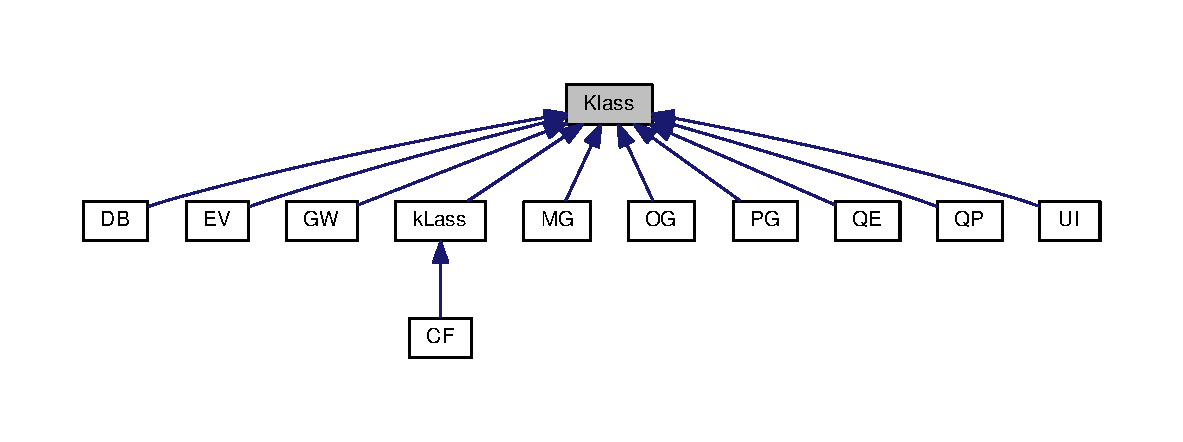
\includegraphics[width=350pt]{class_k_1_1_klass__inherit__graph}
\end{center}
\end{figure}


Collaboration diagram for Klass\+:
\nopagebreak
\begin{figure}[H]
\begin{center}
\leavevmode
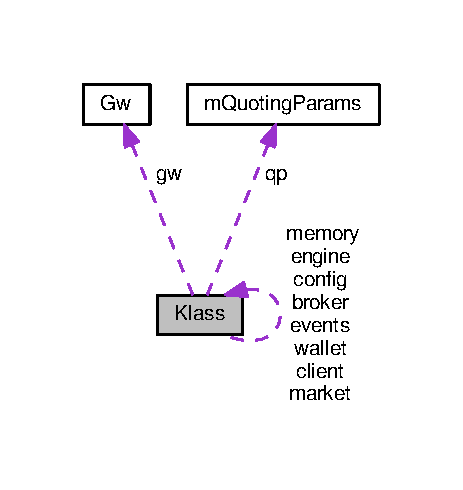
\includegraphics[width=222pt]{class_k_1_1_klass__coll__graph}
\end{center}
\end{figure}
\subsection*{Public Member Functions}
\begin{DoxyCompactItemize}
\item 
void \hyperlink{class_k_1_1_klass_a70db8bd1d499619f7ff9c1ca2ff3c8df}{main} (int argc, char $\ast$$\ast$argv)
\item 
void \hyperlink{class_k_1_1_klass_aa3b21853f890838c88d047d6c2786917}{wait} ()
\item 
void \hyperlink{class_k_1_1_klass_ae5e4326dac127aa27fb0456657a9f49c}{gw\+Link} (\hyperlink{class_k_1_1_gw}{Gw} $\ast$k)
\item 
void \hyperlink{class_k_1_1_klass_a2d610572e6c73a1b702ada2e878a947c}{qp\+Link} (\hyperlink{struct_k_1_1m_quoting_params}{m\+Quoting\+Params} $\ast$k)
\item 
void \hyperlink{class_k_1_1_klass_a39b2f3998c689b256683fd17a651064b}{sh\+Link} (void $\ast$k)
\item 
void \hyperlink{class_k_1_1_klass_ad41a4f32fb16b477ff5bd12ed6e832fa}{cf\+Link} (\hyperlink{class_k_1_1_klass}{Klass} \&k)
\item 
void \hyperlink{class_k_1_1_klass_a07cc2e2fb5c51342a2488d3011d08898}{ev\+Link} (\hyperlink{class_k_1_1_klass}{Klass} \&k)
\item 
void \hyperlink{class_k_1_1_klass_ab0f3d3683bdcb890246728071d683b15}{db\+Link} (\hyperlink{class_k_1_1_klass}{Klass} \&k)
\item 
void \hyperlink{class_k_1_1_klass_aabe268d262e8fbb2210944cbfbb04fb6}{ui\+Link} (\hyperlink{class_k_1_1_klass}{Klass} \&k)
\item 
void \hyperlink{class_k_1_1_klass_ab0a07660f3119715c50624b502227de0}{og\+Link} (\hyperlink{class_k_1_1_klass}{Klass} \&k)
\item 
void \hyperlink{class_k_1_1_klass_a2dbe67fd13e13f6f65f66609b74870d9}{mg\+Link} (\hyperlink{class_k_1_1_klass}{Klass} \&k)
\item 
void \hyperlink{class_k_1_1_klass_a94f13606ea1cae0d00b5d7dce2feda38}{pg\+Link} (\hyperlink{class_k_1_1_klass}{Klass} \&k)
\item 
void \hyperlink{class_k_1_1_klass_a407bab1bd4f3c1511ab8d8f97d7dc78e}{qe\+Link} (\hyperlink{class_k_1_1_klass}{Klass} \&k)
\end{DoxyCompactItemize}
\subsection*{Protected Member Functions}
\begin{DoxyCompactItemize}
\item 
virtual void \hyperlink{class_k_1_1_klass_af62dc66ce38ed384a91677aa1485eb1f}{load} (int argc, char $\ast$$\ast$argv)
\item 
virtual void \hyperlink{class_k_1_1_klass_a5588964fff1d1025245d134e159b60ee}{load} ()
\item 
virtual void \hyperlink{class_k_1_1_klass_a62a6bf36d7c8bec9dcf7af20c9d21d74}{wait\+Data} ()
\item 
virtual void \hyperlink{class_k_1_1_klass_a60afdc2eaa268d8c41a2d6897fbf4fff}{wait\+Time} ()
\item 
virtual void \hyperlink{class_k_1_1_klass_af4f5201bed25a292d8a7f40470d83923}{wait\+User} ()
\item 
virtual void \hyperlink{class_k_1_1_klass_a72fcb26a14f6beb1c3fbace9ab3e7dbb}{run} ()
\end{DoxyCompactItemize}
\subsection*{Protected Attributes}
\begin{DoxyCompactItemize}
\item 
\hyperlink{class_k_1_1_gw}{Gw} $\ast$ \hyperlink{class_k_1_1_klass_a1cc87ecfd597953b3774a8e1fa4c25ec}{gw} = nullptr
\item 
\hyperlink{struct_k_1_1m_quoting_params}{m\+Quoting\+Params} $\ast$ \hyperlink{class_k_1_1_klass_a4554a7ffab1a73a5d43f13b9ac54ffb1}{qp} = nullptr
\item 
void $\ast$ \hyperlink{class_k_1_1_klass_a5819639653d62dde47c40c9d0c06f7ac}{screen} = nullptr
\item 
\hyperlink{class_k_1_1_klass}{Klass} $\ast$ \hyperlink{class_k_1_1_klass_a50e6a746d37cecad79ebeabcb5677722}{config} = nullptr
\item 
\hyperlink{class_k_1_1_klass}{Klass} $\ast$ \hyperlink{class_k_1_1_klass_aef02c650240e6291d8a616cda222d890}{events} = nullptr
\item 
\hyperlink{class_k_1_1_klass}{Klass} $\ast$ \hyperlink{class_k_1_1_klass_afe23c0cbde1ef3bc79fdd6e56f9c120a}{memory} = nullptr
\item 
\hyperlink{class_k_1_1_klass}{Klass} $\ast$ \hyperlink{class_k_1_1_klass_ad64d722352731ddedb64ba82179e0eaa}{client} = nullptr
\item 
\hyperlink{class_k_1_1_klass}{Klass} $\ast$ \hyperlink{class_k_1_1_klass_a48fc03cfcc056aaefb1811e35942008f}{broker} = nullptr
\item 
\hyperlink{class_k_1_1_klass}{Klass} $\ast$ \hyperlink{class_k_1_1_klass_a98dbde943a8c48f1f266b879e5409777}{market} = nullptr
\item 
\hyperlink{class_k_1_1_klass}{Klass} $\ast$ \hyperlink{class_k_1_1_klass_a5943d9c958085108c746fdc756c7aad3}{wallet} = nullptr
\item 
\hyperlink{class_k_1_1_klass}{Klass} $\ast$ \hyperlink{class_k_1_1_klass_ad2746d88e168f466f52cdf9e07f67ab1}{engine} = nullptr
\end{DoxyCompactItemize}


\subsection{Detailed Description}


Definition at line 729 of file km.\+h.



\subsection{Member Function Documentation}
\index{K\+::\+Klass@{K\+::\+Klass}!cf\+Link@{cf\+Link}}
\index{cf\+Link@{cf\+Link}!K\+::\+Klass@{K\+::\+Klass}}
\subsubsection[{\texorpdfstring{cf\+Link(\+Klass \&k)}{cfLink(Klass &k)}}]{\setlength{\rightskip}{0pt plus 5cm}void cf\+Link (
\begin{DoxyParamCaption}
\item[{{\bf Klass} \&}]{k}
\end{DoxyParamCaption}
)\hspace{0.3cm}{\ttfamily [inline]}}\hypertarget{class_k_1_1_klass_ad41a4f32fb16b477ff5bd12ed6e832fa}{}\label{class_k_1_1_klass_ad41a4f32fb16b477ff5bd12ed6e832fa}


Definition at line 763 of file km.\+h.

\index{K\+::\+Klass@{K\+::\+Klass}!db\+Link@{db\+Link}}
\index{db\+Link@{db\+Link}!K\+::\+Klass@{K\+::\+Klass}}
\subsubsection[{\texorpdfstring{db\+Link(\+Klass \&k)}{dbLink(Klass &k)}}]{\setlength{\rightskip}{0pt plus 5cm}void db\+Link (
\begin{DoxyParamCaption}
\item[{{\bf Klass} \&}]{k}
\end{DoxyParamCaption}
)\hspace{0.3cm}{\ttfamily [inline]}}\hypertarget{class_k_1_1_klass_ab0f3d3683bdcb890246728071d683b15}{}\label{class_k_1_1_klass_ab0f3d3683bdcb890246728071d683b15}


Definition at line 765 of file km.\+h.

\index{K\+::\+Klass@{K\+::\+Klass}!ev\+Link@{ev\+Link}}
\index{ev\+Link@{ev\+Link}!K\+::\+Klass@{K\+::\+Klass}}
\subsubsection[{\texorpdfstring{ev\+Link(\+Klass \&k)}{evLink(Klass &k)}}]{\setlength{\rightskip}{0pt plus 5cm}void ev\+Link (
\begin{DoxyParamCaption}
\item[{{\bf Klass} \&}]{k}
\end{DoxyParamCaption}
)\hspace{0.3cm}{\ttfamily [inline]}}\hypertarget{class_k_1_1_klass_a07cc2e2fb5c51342a2488d3011d08898}{}\label{class_k_1_1_klass_a07cc2e2fb5c51342a2488d3011d08898}


Definition at line 764 of file km.\+h.

\index{K\+::\+Klass@{K\+::\+Klass}!gw\+Link@{gw\+Link}}
\index{gw\+Link@{gw\+Link}!K\+::\+Klass@{K\+::\+Klass}}
\subsubsection[{\texorpdfstring{gw\+Link(\+Gw $\ast$k)}{gwLink(Gw *k)}}]{\setlength{\rightskip}{0pt plus 5cm}void gw\+Link (
\begin{DoxyParamCaption}
\item[{{\bf Gw} $\ast$}]{k}
\end{DoxyParamCaption}
)\hspace{0.3cm}{\ttfamily [inline]}}\hypertarget{class_k_1_1_klass_ae5e4326dac127aa27fb0456657a9f49c}{}\label{class_k_1_1_klass_ae5e4326dac127aa27fb0456657a9f49c}


Definition at line 760 of file km.\+h.

\index{K\+::\+Klass@{K\+::\+Klass}!load@{load}}
\index{load@{load}!K\+::\+Klass@{K\+::\+Klass}}
\subsubsection[{\texorpdfstring{load(int argc, char $\ast$$\ast$argv)}{load(int argc, char **argv)}}]{\setlength{\rightskip}{0pt plus 5cm}virtual void load (
\begin{DoxyParamCaption}
\item[{int}]{argc, }
\item[{char $\ast$$\ast$}]{argv}
\end{DoxyParamCaption}
)\hspace{0.3cm}{\ttfamily [inline]}, {\ttfamily [protected]}, {\ttfamily [virtual]}}\hypertarget{class_k_1_1_klass_af62dc66ce38ed384a91677aa1485eb1f}{}\label{class_k_1_1_klass_af62dc66ce38ed384a91677aa1485eb1f}


Reimplemented in \hyperlink{class_k_1_1_c_f_aa7590ffe947041a741bb86945e1aa572}{CF}.



Definition at line 742 of file km.\+h.

\index{K\+::\+Klass@{K\+::\+Klass}!load@{load}}
\index{load@{load}!K\+::\+Klass@{K\+::\+Klass}}
\subsubsection[{\texorpdfstring{load()}{load()}}]{\setlength{\rightskip}{0pt plus 5cm}virtual void load (
\begin{DoxyParamCaption}
{}
\end{DoxyParamCaption}
)\hspace{0.3cm}{\ttfamily [inline]}, {\ttfamily [protected]}, {\ttfamily [virtual]}}\hypertarget{class_k_1_1_klass_a5588964fff1d1025245d134e159b60ee}{}\label{class_k_1_1_klass_a5588964fff1d1025245d134e159b60ee}


Reimplemented in \hyperlink{class_k_1_1_m_g_a78f61ac2dd03bcba8e09ca20cd7d68e3}{MG}, \hyperlink{class_k_1_1_u_i_a78f61ac2dd03bcba8e09ca20cd7d68e3}{UI}, \hyperlink{class_k_1_1_p_g_a78f61ac2dd03bcba8e09ca20cd7d68e3}{PG}, \hyperlink{class_k_1_1_e_v_a78f61ac2dd03bcba8e09ca20cd7d68e3}{EV}, \hyperlink{class_k_1_1_g_w_a78f61ac2dd03bcba8e09ca20cd7d68e3}{GW}, \hyperlink{class_k_1_1_q_e_a78f61ac2dd03bcba8e09ca20cd7d68e3}{QE}, \hyperlink{class_k_1_1_d_b_a78f61ac2dd03bcba8e09ca20cd7d68e3}{DB}, \hyperlink{class_k_1_1_o_g_a78f61ac2dd03bcba8e09ca20cd7d68e3}{OG}, and \hyperlink{class_k_1_1_q_p_a78f61ac2dd03bcba8e09ca20cd7d68e3}{QP}.



Definition at line 743 of file km.\+h.

\index{K\+::\+Klass@{K\+::\+Klass}!main@{main}}
\index{main@{main}!K\+::\+Klass@{K\+::\+Klass}}
\subsubsection[{\texorpdfstring{main(int argc, char $\ast$$\ast$argv)}{main(int argc, char **argv)}}]{\setlength{\rightskip}{0pt plus 5cm}void main (
\begin{DoxyParamCaption}
\item[{int}]{argc, }
\item[{char $\ast$$\ast$}]{argv}
\end{DoxyParamCaption}
)\hspace{0.3cm}{\ttfamily [inline]}}\hypertarget{class_k_1_1_klass_a70db8bd1d499619f7ff9c1ca2ff3c8df}{}\label{class_k_1_1_klass_a70db8bd1d499619f7ff9c1ca2ff3c8df}


Definition at line 749 of file km.\+h.

\index{K\+::\+Klass@{K\+::\+Klass}!mg\+Link@{mg\+Link}}
\index{mg\+Link@{mg\+Link}!K\+::\+Klass@{K\+::\+Klass}}
\subsubsection[{\texorpdfstring{mg\+Link(\+Klass \&k)}{mgLink(Klass &k)}}]{\setlength{\rightskip}{0pt plus 5cm}void mg\+Link (
\begin{DoxyParamCaption}
\item[{{\bf Klass} \&}]{k}
\end{DoxyParamCaption}
)\hspace{0.3cm}{\ttfamily [inline]}}\hypertarget{class_k_1_1_klass_a2dbe67fd13e13f6f65f66609b74870d9}{}\label{class_k_1_1_klass_a2dbe67fd13e13f6f65f66609b74870d9}


Definition at line 768 of file km.\+h.

\index{K\+::\+Klass@{K\+::\+Klass}!og\+Link@{og\+Link}}
\index{og\+Link@{og\+Link}!K\+::\+Klass@{K\+::\+Klass}}
\subsubsection[{\texorpdfstring{og\+Link(\+Klass \&k)}{ogLink(Klass &k)}}]{\setlength{\rightskip}{0pt plus 5cm}void og\+Link (
\begin{DoxyParamCaption}
\item[{{\bf Klass} \&}]{k}
\end{DoxyParamCaption}
)\hspace{0.3cm}{\ttfamily [inline]}}\hypertarget{class_k_1_1_klass_ab0a07660f3119715c50624b502227de0}{}\label{class_k_1_1_klass_ab0a07660f3119715c50624b502227de0}


Definition at line 767 of file km.\+h.

\index{K\+::\+Klass@{K\+::\+Klass}!pg\+Link@{pg\+Link}}
\index{pg\+Link@{pg\+Link}!K\+::\+Klass@{K\+::\+Klass}}
\subsubsection[{\texorpdfstring{pg\+Link(\+Klass \&k)}{pgLink(Klass &k)}}]{\setlength{\rightskip}{0pt plus 5cm}void pg\+Link (
\begin{DoxyParamCaption}
\item[{{\bf Klass} \&}]{k}
\end{DoxyParamCaption}
)\hspace{0.3cm}{\ttfamily [inline]}}\hypertarget{class_k_1_1_klass_a94f13606ea1cae0d00b5d7dce2feda38}{}\label{class_k_1_1_klass_a94f13606ea1cae0d00b5d7dce2feda38}


Definition at line 769 of file km.\+h.

\index{K\+::\+Klass@{K\+::\+Klass}!qe\+Link@{qe\+Link}}
\index{qe\+Link@{qe\+Link}!K\+::\+Klass@{K\+::\+Klass}}
\subsubsection[{\texorpdfstring{qe\+Link(\+Klass \&k)}{qeLink(Klass &k)}}]{\setlength{\rightskip}{0pt plus 5cm}void qe\+Link (
\begin{DoxyParamCaption}
\item[{{\bf Klass} \&}]{k}
\end{DoxyParamCaption}
)\hspace{0.3cm}{\ttfamily [inline]}}\hypertarget{class_k_1_1_klass_a407bab1bd4f3c1511ab8d8f97d7dc78e}{}\label{class_k_1_1_klass_a407bab1bd4f3c1511ab8d8f97d7dc78e}


Definition at line 770 of file km.\+h.

\index{K\+::\+Klass@{K\+::\+Klass}!qp\+Link@{qp\+Link}}
\index{qp\+Link@{qp\+Link}!K\+::\+Klass@{K\+::\+Klass}}
\subsubsection[{\texorpdfstring{qp\+Link(m\+Quoting\+Params $\ast$k)}{qpLink(mQuotingParams *k)}}]{\setlength{\rightskip}{0pt plus 5cm}void qp\+Link (
\begin{DoxyParamCaption}
\item[{{\bf m\+Quoting\+Params} $\ast$}]{k}
\end{DoxyParamCaption}
)\hspace{0.3cm}{\ttfamily [inline]}}\hypertarget{class_k_1_1_klass_a2d610572e6c73a1b702ada2e878a947c}{}\label{class_k_1_1_klass_a2d610572e6c73a1b702ada2e878a947c}


Definition at line 761 of file km.\+h.

\index{K\+::\+Klass@{K\+::\+Klass}!run@{run}}
\index{run@{run}!K\+::\+Klass@{K\+::\+Klass}}
\subsubsection[{\texorpdfstring{run()}{run()}}]{\setlength{\rightskip}{0pt plus 5cm}virtual void run (
\begin{DoxyParamCaption}
{}
\end{DoxyParamCaption}
)\hspace{0.3cm}{\ttfamily [inline]}, {\ttfamily [protected]}, {\ttfamily [virtual]}}\hypertarget{class_k_1_1_klass_a72fcb26a14f6beb1c3fbace9ab3e7dbb}{}\label{class_k_1_1_klass_a72fcb26a14f6beb1c3fbace9ab3e7dbb}


Reimplemented in \hyperlink{class_k_1_1_c_f_a13a43e6d814de94978c515cb084873b1}{CF}, \hyperlink{class_k_1_1_u_i_a13a43e6d814de94978c515cb084873b1}{UI}, \hyperlink{class_k_1_1_g_w_a13a43e6d814de94978c515cb084873b1}{GW}, \hyperlink{class_k_1_1_e_v_a13a43e6d814de94978c515cb084873b1}{EV}, \hyperlink{class_k_1_1_o_g_a13a43e6d814de94978c515cb084873b1}{OG}, \hyperlink{class_k_1_1_q_e_a13a43e6d814de94978c515cb084873b1}{QE}, \hyperlink{class_k_1_1_d_b_a13a43e6d814de94978c515cb084873b1}{DB}, and \hyperlink{class_k_1_1_q_p_a13a43e6d814de94978c515cb084873b1}{QP}.



Definition at line 747 of file km.\+h.

\index{K\+::\+Klass@{K\+::\+Klass}!sh\+Link@{sh\+Link}}
\index{sh\+Link@{sh\+Link}!K\+::\+Klass@{K\+::\+Klass}}
\subsubsection[{\texorpdfstring{sh\+Link(void $\ast$k)}{shLink(void *k)}}]{\setlength{\rightskip}{0pt plus 5cm}void sh\+Link (
\begin{DoxyParamCaption}
\item[{void $\ast$}]{k}
\end{DoxyParamCaption}
)\hspace{0.3cm}{\ttfamily [inline]}}\hypertarget{class_k_1_1_klass_a39b2f3998c689b256683fd17a651064b}{}\label{class_k_1_1_klass_a39b2f3998c689b256683fd17a651064b}


Definition at line 762 of file km.\+h.

\index{K\+::\+Klass@{K\+::\+Klass}!ui\+Link@{ui\+Link}}
\index{ui\+Link@{ui\+Link}!K\+::\+Klass@{K\+::\+Klass}}
\subsubsection[{\texorpdfstring{ui\+Link(\+Klass \&k)}{uiLink(Klass &k)}}]{\setlength{\rightskip}{0pt plus 5cm}void ui\+Link (
\begin{DoxyParamCaption}
\item[{{\bf Klass} \&}]{k}
\end{DoxyParamCaption}
)\hspace{0.3cm}{\ttfamily [inline]}}\hypertarget{class_k_1_1_klass_aabe268d262e8fbb2210944cbfbb04fb6}{}\label{class_k_1_1_klass_aabe268d262e8fbb2210944cbfbb04fb6}


Definition at line 766 of file km.\+h.

\index{K\+::\+Klass@{K\+::\+Klass}!wait@{wait}}
\index{wait@{wait}!K\+::\+Klass@{K\+::\+Klass}}
\subsubsection[{\texorpdfstring{wait()}{wait()}}]{\setlength{\rightskip}{0pt plus 5cm}void wait (
\begin{DoxyParamCaption}
{}
\end{DoxyParamCaption}
)\hspace{0.3cm}{\ttfamily [inline]}}\hypertarget{class_k_1_1_klass_aa3b21853f890838c88d047d6c2786917}{}\label{class_k_1_1_klass_aa3b21853f890838c88d047d6c2786917}


Definition at line 753 of file km.\+h.

\index{K\+::\+Klass@{K\+::\+Klass}!wait\+Data@{wait\+Data}}
\index{wait\+Data@{wait\+Data}!K\+::\+Klass@{K\+::\+Klass}}
\subsubsection[{\texorpdfstring{wait\+Data()}{waitData()}}]{\setlength{\rightskip}{0pt plus 5cm}virtual void wait\+Data (
\begin{DoxyParamCaption}
{}
\end{DoxyParamCaption}
)\hspace{0.3cm}{\ttfamily [inline]}, {\ttfamily [protected]}, {\ttfamily [virtual]}}\hypertarget{class_k_1_1_klass_a62a6bf36d7c8bec9dcf7af20c9d21d74}{}\label{class_k_1_1_klass_a62a6bf36d7c8bec9dcf7af20c9d21d74}


Reimplemented in \hyperlink{class_k_1_1_m_g_aa9a0f090ee360e2a9f967200d30f4a22}{MG}, \hyperlink{class_k_1_1_p_g_aa9a0f090ee360e2a9f967200d30f4a22}{PG}, \hyperlink{class_k_1_1_u_i_aa9a0f090ee360e2a9f967200d30f4a22}{UI}, \hyperlink{class_k_1_1_e_v_aa9a0f090ee360e2a9f967200d30f4a22}{EV}, \hyperlink{class_k_1_1_q_e_aa9a0f090ee360e2a9f967200d30f4a22}{QE}, \hyperlink{class_k_1_1_g_w_aa9a0f090ee360e2a9f967200d30f4a22}{GW}, and \hyperlink{class_k_1_1_o_g_aa9a0f090ee360e2a9f967200d30f4a22}{OG}.



Definition at line 744 of file km.\+h.

\index{K\+::\+Klass@{K\+::\+Klass}!wait\+Time@{wait\+Time}}
\index{wait\+Time@{wait\+Time}!K\+::\+Klass@{K\+::\+Klass}}
\subsubsection[{\texorpdfstring{wait\+Time()}{waitTime()}}]{\setlength{\rightskip}{0pt plus 5cm}virtual void wait\+Time (
\begin{DoxyParamCaption}
{}
\end{DoxyParamCaption}
)\hspace{0.3cm}{\ttfamily [inline]}, {\ttfamily [protected]}, {\ttfamily [virtual]}}\hypertarget{class_k_1_1_klass_a60afdc2eaa268d8c41a2d6897fbf4fff}{}\label{class_k_1_1_klass_a60afdc2eaa268d8c41a2d6897fbf4fff}


Reimplemented in \hyperlink{class_k_1_1_u_i_ade4c89163dbda531e71c8c75eb2868b4}{UI}, \hyperlink{class_k_1_1_e_v_ade4c89163dbda531e71c8c75eb2868b4}{EV}, and \hyperlink{class_k_1_1_g_w_ade4c89163dbda531e71c8c75eb2868b4}{GW}.



Definition at line 745 of file km.\+h.

\index{K\+::\+Klass@{K\+::\+Klass}!wait\+User@{wait\+User}}
\index{wait\+User@{wait\+User}!K\+::\+Klass@{K\+::\+Klass}}
\subsubsection[{\texorpdfstring{wait\+User()}{waitUser()}}]{\setlength{\rightskip}{0pt plus 5cm}virtual void wait\+User (
\begin{DoxyParamCaption}
{}
\end{DoxyParamCaption}
)\hspace{0.3cm}{\ttfamily [inline]}, {\ttfamily [protected]}, {\ttfamily [virtual]}}\hypertarget{class_k_1_1_klass_af4f5201bed25a292d8a7f40470d83923}{}\label{class_k_1_1_klass_af4f5201bed25a292d8a7f40470d83923}


Reimplemented in \hyperlink{class_k_1_1_u_i_aa3f7b56799f5915cfbc902f6426c2bb2}{UI}, \hyperlink{class_k_1_1_m_g_aa3f7b56799f5915cfbc902f6426c2bb2}{MG}, \hyperlink{class_k_1_1_g_w_aa3f7b56799f5915cfbc902f6426c2bb2}{GW}, \hyperlink{class_k_1_1_p_g_aa3f7b56799f5915cfbc902f6426c2bb2}{PG}, \hyperlink{class_k_1_1_e_v_aa3f7b56799f5915cfbc902f6426c2bb2}{EV}, \hyperlink{class_k_1_1_q_e_aa3f7b56799f5915cfbc902f6426c2bb2}{QE}, \hyperlink{class_k_1_1_o_g_aa3f7b56799f5915cfbc902f6426c2bb2}{OG}, and \hyperlink{class_k_1_1_q_p_aa3f7b56799f5915cfbc902f6426c2bb2}{QP}.



Definition at line 746 of file km.\+h.



\subsection{Field Documentation}
\index{K\+::\+Klass@{K\+::\+Klass}!broker@{broker}}
\index{broker@{broker}!K\+::\+Klass@{K\+::\+Klass}}
\subsubsection[{\texorpdfstring{broker}{broker}}]{\setlength{\rightskip}{0pt plus 5cm}{\bf Klass} $\ast$ broker = nullptr\hspace{0.3cm}{\ttfamily [protected]}}\hypertarget{class_k_1_1_klass_a48fc03cfcc056aaefb1811e35942008f}{}\label{class_k_1_1_klass_a48fc03cfcc056aaefb1811e35942008f}


Definition at line 738 of file km.\+h.

\index{K\+::\+Klass@{K\+::\+Klass}!client@{client}}
\index{client@{client}!K\+::\+Klass@{K\+::\+Klass}}
\subsubsection[{\texorpdfstring{client}{client}}]{\setlength{\rightskip}{0pt plus 5cm}{\bf Klass} $\ast$ client = nullptr\hspace{0.3cm}{\ttfamily [protected]}}\hypertarget{class_k_1_1_klass_ad64d722352731ddedb64ba82179e0eaa}{}\label{class_k_1_1_klass_ad64d722352731ddedb64ba82179e0eaa}


Definition at line 737 of file km.\+h.

\index{K\+::\+Klass@{K\+::\+Klass}!config@{config}}
\index{config@{config}!K\+::\+Klass@{K\+::\+Klass}}
\subsubsection[{\texorpdfstring{config}{config}}]{\setlength{\rightskip}{0pt plus 5cm}{\bf Klass}$\ast$ config = nullptr\hspace{0.3cm}{\ttfamily [protected]}}\hypertarget{class_k_1_1_klass_a50e6a746d37cecad79ebeabcb5677722}{}\label{class_k_1_1_klass_a50e6a746d37cecad79ebeabcb5677722}


Definition at line 734 of file km.\+h.

\index{K\+::\+Klass@{K\+::\+Klass}!engine@{engine}}
\index{engine@{engine}!K\+::\+Klass@{K\+::\+Klass}}
\subsubsection[{\texorpdfstring{engine}{engine}}]{\setlength{\rightskip}{0pt plus 5cm}{\bf Klass} $\ast$ engine = nullptr\hspace{0.3cm}{\ttfamily [protected]}}\hypertarget{class_k_1_1_klass_ad2746d88e168f466f52cdf9e07f67ab1}{}\label{class_k_1_1_klass_ad2746d88e168f466f52cdf9e07f67ab1}


Definition at line 741 of file km.\+h.

\index{K\+::\+Klass@{K\+::\+Klass}!events@{events}}
\index{events@{events}!K\+::\+Klass@{K\+::\+Klass}}
\subsubsection[{\texorpdfstring{events}{events}}]{\setlength{\rightskip}{0pt plus 5cm}{\bf Klass} $\ast$ events = nullptr\hspace{0.3cm}{\ttfamily [protected]}}\hypertarget{class_k_1_1_klass_aef02c650240e6291d8a616cda222d890}{}\label{class_k_1_1_klass_aef02c650240e6291d8a616cda222d890}


Definition at line 735 of file km.\+h.

\index{K\+::\+Klass@{K\+::\+Klass}!gw@{gw}}
\index{gw@{gw}!K\+::\+Klass@{K\+::\+Klass}}
\subsubsection[{\texorpdfstring{gw}{gw}}]{\setlength{\rightskip}{0pt plus 5cm}{\bf Gw}$\ast$ gw = nullptr\hspace{0.3cm}{\ttfamily [protected]}}\hypertarget{class_k_1_1_klass_a1cc87ecfd597953b3774a8e1fa4c25ec}{}\label{class_k_1_1_klass_a1cc87ecfd597953b3774a8e1fa4c25ec}


Definition at line 731 of file km.\+h.

\index{K\+::\+Klass@{K\+::\+Klass}!market@{market}}
\index{market@{market}!K\+::\+Klass@{K\+::\+Klass}}
\subsubsection[{\texorpdfstring{market}{market}}]{\setlength{\rightskip}{0pt plus 5cm}{\bf Klass} $\ast$ market = nullptr\hspace{0.3cm}{\ttfamily [protected]}}\hypertarget{class_k_1_1_klass_a98dbde943a8c48f1f266b879e5409777}{}\label{class_k_1_1_klass_a98dbde943a8c48f1f266b879e5409777}


Definition at line 739 of file km.\+h.

\index{K\+::\+Klass@{K\+::\+Klass}!memory@{memory}}
\index{memory@{memory}!K\+::\+Klass@{K\+::\+Klass}}
\subsubsection[{\texorpdfstring{memory}{memory}}]{\setlength{\rightskip}{0pt plus 5cm}{\bf Klass} $\ast$ memory = nullptr\hspace{0.3cm}{\ttfamily [protected]}}\hypertarget{class_k_1_1_klass_afe23c0cbde1ef3bc79fdd6e56f9c120a}{}\label{class_k_1_1_klass_afe23c0cbde1ef3bc79fdd6e56f9c120a}


Definition at line 736 of file km.\+h.

\index{K\+::\+Klass@{K\+::\+Klass}!qp@{qp}}
\index{qp@{qp}!K\+::\+Klass@{K\+::\+Klass}}
\subsubsection[{\texorpdfstring{qp}{qp}}]{\setlength{\rightskip}{0pt plus 5cm}{\bf m\+Quoting\+Params}$\ast$ qp = nullptr\hspace{0.3cm}{\ttfamily [protected]}}\hypertarget{class_k_1_1_klass_a4554a7ffab1a73a5d43f13b9ac54ffb1}{}\label{class_k_1_1_klass_a4554a7ffab1a73a5d43f13b9ac54ffb1}


Definition at line 732 of file km.\+h.

\index{K\+::\+Klass@{K\+::\+Klass}!screen@{screen}}
\index{screen@{screen}!K\+::\+Klass@{K\+::\+Klass}}
\subsubsection[{\texorpdfstring{screen}{screen}}]{\setlength{\rightskip}{0pt plus 5cm}void$\ast$ screen = nullptr\hspace{0.3cm}{\ttfamily [protected]}}\hypertarget{class_k_1_1_klass_a5819639653d62dde47c40c9d0c06f7ac}{}\label{class_k_1_1_klass_a5819639653d62dde47c40c9d0c06f7ac}


Definition at line 733 of file km.\+h.

\index{K\+::\+Klass@{K\+::\+Klass}!wallet@{wallet}}
\index{wallet@{wallet}!K\+::\+Klass@{K\+::\+Klass}}
\subsubsection[{\texorpdfstring{wallet}{wallet}}]{\setlength{\rightskip}{0pt plus 5cm}{\bf Klass} $\ast$ wallet = nullptr\hspace{0.3cm}{\ttfamily [protected]}}\hypertarget{class_k_1_1_klass_a5943d9c958085108c746fdc756c7aad3}{}\label{class_k_1_1_klass_a5943d9c958085108c746fdc756c7aad3}


Definition at line 740 of file km.\+h.



The documentation for this class was generated from the following file\+:\begin{DoxyCompactItemize}
\item 
\hyperlink{km_8h}{km.\+h}\end{DoxyCompactItemize}

\hypertarget{class_k_1_1k_lass}{}\section{k\+Lass Class Reference}
\label{class_k_1_1k_lass}\index{k\+Lass@{k\+Lass}}


{\ttfamily \#include $<$km.\+h$>$}



Inheritance diagram for k\+Lass\+:
\nopagebreak
\begin{figure}[H]
\begin{center}
\leavevmode
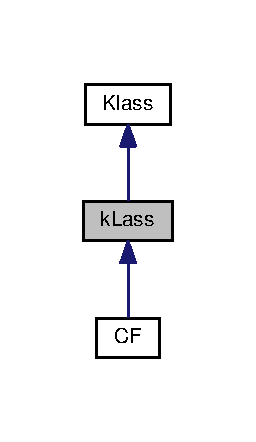
\includegraphics[width=123pt]{class_k_1_1k_lass__inherit__graph}
\end{center}
\end{figure}


Collaboration diagram for k\+Lass\+:
\nopagebreak
\begin{figure}[H]
\begin{center}
\leavevmode
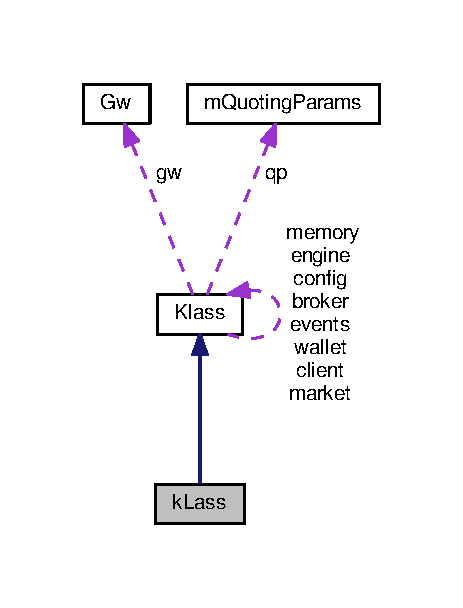
\includegraphics[width=222pt]{class_k_1_1k_lass__coll__graph}
\end{center}
\end{figure}
\subsection*{Public Member Functions}
\begin{DoxyCompactItemize}
\item 
void \hyperlink{class_k_1_1k_lass_a1407574ee891838953937aa7cd68ec6b}{link} (\hyperlink{class_k_1_1_klass}{Klass} \&\hyperlink{class_k_1_1_e_v}{EV}, \hyperlink{class_k_1_1_klass}{Klass} \&\hyperlink{class_k_1_1_d_b}{DB}, \hyperlink{class_k_1_1_klass}{Klass} \&\hyperlink{class_k_1_1_u_i}{UI}, \hyperlink{class_k_1_1_klass}{Klass} \&\hyperlink{class_k_1_1_q_p}{QP}, \hyperlink{class_k_1_1_klass}{Klass} \&\hyperlink{class_k_1_1_o_g}{OG}, \hyperlink{class_k_1_1_klass}{Klass} \&\hyperlink{class_k_1_1_m_g}{MG}, \hyperlink{class_k_1_1_klass}{Klass} \&\hyperlink{class_k_1_1_p_g}{PG}, \hyperlink{class_k_1_1_klass}{Klass} \&\hyperlink{class_k_1_1_q_e}{QE}, \hyperlink{class_k_1_1_klass}{Klass} \&\hyperlink{class_k_1_1_g_w}{GW})
\end{DoxyCompactItemize}
\subsection*{Additional Inherited Members}


\subsection{Detailed Description}


Definition at line 772 of file km.\+h.



\subsection{Member Function Documentation}
\index{K\+::k\+Lass@{K\+::k\+Lass}!link@{link}}
\index{link@{link}!K\+::k\+Lass@{K\+::k\+Lass}}
\subsubsection[{\texorpdfstring{link(\+Klass \&\+E\+V, Klass \&\+D\+B, Klass \&\+U\+I, Klass \&\+Q\+P, Klass \&\+O\+G, Klass \&\+M\+G, Klass \&\+P\+G, Klass \&\+Q\+E, Klass \&\+G\+W)}{link(Klass &EV, Klass &DB, Klass &UI, Klass &QP, Klass &OG, Klass &MG, Klass &PG, Klass &QE, Klass &GW)}}]{\setlength{\rightskip}{0pt plus 5cm}void link (
\begin{DoxyParamCaption}
\item[{{\bf Klass} \&}]{EV, }
\item[{{\bf Klass} \&}]{DB, }
\item[{{\bf Klass} \&}]{UI, }
\item[{{\bf Klass} \&}]{QP, }
\item[{{\bf Klass} \&}]{OG, }
\item[{{\bf Klass} \&}]{MG, }
\item[{{\bf Klass} \&}]{PG, }
\item[{{\bf Klass} \&}]{QE, }
\item[{{\bf Klass} \&}]{GW}
\end{DoxyParamCaption}
)\hspace{0.3cm}{\ttfamily [inline]}}\hypertarget{class_k_1_1k_lass_a1407574ee891838953937aa7cd68ec6b}{}\label{class_k_1_1k_lass_a1407574ee891838953937aa7cd68ec6b}


Definition at line 776 of file km.\+h.



The documentation for this class was generated from the following file\+:\begin{DoxyCompactItemize}
\item 
\hyperlink{km_8h}{km.\+h}\end{DoxyCompactItemize}

\hypertarget{class_k_1_1_m_g}{}\section{MG Class Reference}
\label{class_k_1_1_m_g}\index{MG@{MG}}


{\ttfamily \#include $<$mg.\+h$>$}



Inheritance diagram for MG\+:
\nopagebreak
\begin{figure}[H]
\begin{center}
\leavevmode
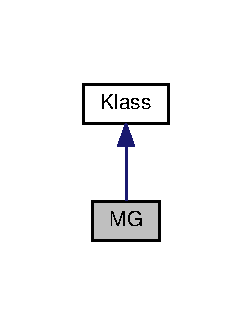
\includegraphics[width=121pt]{class_k_1_1_m_g__inherit__graph}
\end{center}
\end{figure}


Collaboration diagram for MG\+:
\nopagebreak
\begin{figure}[H]
\begin{center}
\leavevmode
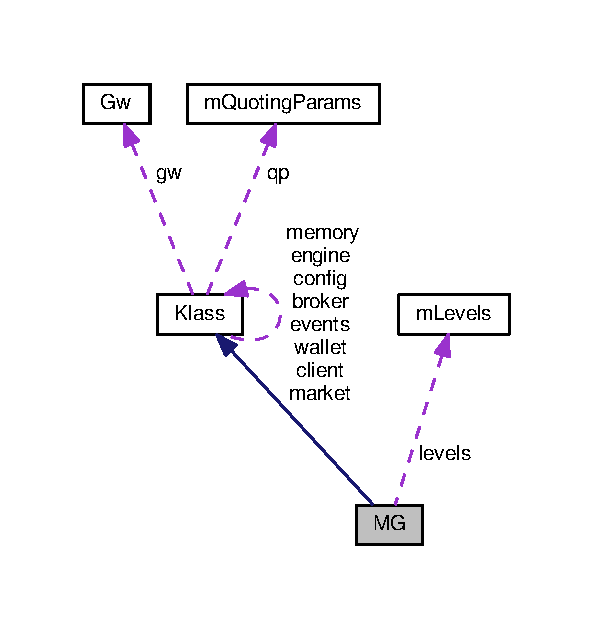
\includegraphics[width=285pt]{class_k_1_1_m_g__coll__graph}
\end{center}
\end{figure}
\subsection*{Public Member Functions}
\begin{DoxyCompactItemize}
\item 
void \hyperlink{class_k_1_1_m_g_a785796c4aff2e5bddf071efeb14a5f8a}{calc\+Stats} ()
\item 
void \hyperlink{class_k_1_1_m_g_a015722c233590fa0304b0459417dfc6b}{calc\+Fair\+Value} ()
\item 
void \hyperlink{class_k_1_1_m_g_aad02ad8dba997ebd2f1e03a94d7b8633}{calc\+Ewma\+History} ()
\end{DoxyCompactItemize}
\subsection*{Data Fields}
\begin{DoxyCompactItemize}
\item 
function$<$ void()$>$ $\ast$ \hyperlink{class_k_1_1_m_g_a62d2cf6a8a40f2b9f3671e89416b09e1}{calc\+Quote} = nullptr
\item 
function$<$ void()$>$ $\ast$ \hyperlink{class_k_1_1_m_g_a427f330e901dc47bf84fd9fe98590924}{calc\+Target\+Base\+Pos} = nullptr
\item 
\hyperlink{struct_k_1_1m_levels}{m\+Levels} \hyperlink{class_k_1_1_m_g_a1ff20b3cba9c009511bea1c21952a5ee}{levels}
\item 
\hyperlink{km_8h_a392f9b7f384aa3539bbb890b059f5b8c}{m\+Price} \hyperlink{class_k_1_1_m_g_a68046d94c62e77cce36ea7de25b7927d}{fair\+Value} = 0
\item 
\hyperlink{km_8h_a392f9b7f384aa3539bbb890b059f5b8c}{m\+Price} \hyperlink{class_k_1_1_m_g_ae990143af8448b62f44b2b2d7787eebc}{mg\+EwmaP} = 0
\item 
\hyperlink{km_8h_a392f9b7f384aa3539bbb890b059f5b8c}{m\+Price} \hyperlink{class_k_1_1_m_g_ad9e670e4f0b6caf6a5a8d8ee23acf178}{mg\+EwmaW} = 0
\item 
double \hyperlink{class_k_1_1_m_g_a413889c063d487f39908c7c777096aa1}{target\+Position} = 0
\item 
double \hyperlink{class_k_1_1_m_g_ac4451d8294cb8944c256971e1acb775b}{mg\+Stdev\+Top} = 0
\item 
double \hyperlink{class_k_1_1_m_g_abf4a6e034d5cf8359ada9f8344b0f469}{mg\+Stdev\+Top\+Mean} = 0
\item 
double \hyperlink{class_k_1_1_m_g_a47f0036553b72247f6754ceddb5c113b}{mg\+Stdev\+FV} = 0
\item 
double \hyperlink{class_k_1_1_m_g_a020f609af7e4ab045b64ca49a8db4f44}{mg\+Stdev\+F\+V\+Mean} = 0
\item 
double \hyperlink{class_k_1_1_m_g_a3c10d311c08f2978192402d961cc32aa}{mg\+Stdev\+Bid} = 0
\item 
double \hyperlink{class_k_1_1_m_g_a6eb5979883c311c60b4c02f8faa20185}{mg\+Stdev\+Bid\+Mean} = 0
\item 
double \hyperlink{class_k_1_1_m_g_a30c5f31a2b624ae505d3b371286a283b}{mg\+Stdev\+Ask} = 0
\item 
double \hyperlink{class_k_1_1_m_g_a573fe2cde6d4be29b8adb62d9c6df216}{mg\+Stdev\+Ask\+Mean} = 0
\item 
double \hyperlink{class_k_1_1_m_g_acd339134ddd47c67ddd7c3a8acdf7b3c}{mg\+Ewma\+Trend\+Diff} = 0
\item 
map$<$ \hyperlink{km_8h_a392f9b7f384aa3539bbb890b059f5b8c}{m\+Price}, \hyperlink{km_8h_ad4d00888c55a47a8a40ed8020d176086}{m\+Amount} $>$ \hyperlink{class_k_1_1_m_g_a7b79b121faa31d26dcd1d6e3fb9a6b24}{filter\+Bid\+Orders}
\item 
map$<$ \hyperlink{km_8h_a392f9b7f384aa3539bbb890b059f5b8c}{m\+Price}, \hyperlink{km_8h_ad4d00888c55a47a8a40ed8020d176086}{m\+Amount} $>$ \hyperlink{class_k_1_1_m_g_aa30d4938235eda21a76452fd71e10ae7}{filter\+Ask\+Orders}
\end{DoxyCompactItemize}
\subsection*{Protected Member Functions}
\begin{DoxyCompactItemize}
\item 
void \hyperlink{class_k_1_1_m_g_a78f61ac2dd03bcba8e09ca20cd7d68e3}{load} ()
\item 
void \hyperlink{class_k_1_1_m_g_aa9a0f090ee360e2a9f967200d30f4a22}{wait\+Data} ()
\item 
void \hyperlink{class_k_1_1_m_g_aa3f7b56799f5915cfbc902f6426c2bb2}{wait\+User} ()
\end{DoxyCompactItemize}
\subsection*{Additional Inherited Members}


\subsection{Detailed Description}


Definition at line 5 of file mg.\+h.



\subsection{Member Function Documentation}
\index{K\+::\+MG@{K\+::\+MG}!calc\+Ewma\+History@{calc\+Ewma\+History}}
\index{calc\+Ewma\+History@{calc\+Ewma\+History}!K\+::\+MG@{K\+::\+MG}}
\subsubsection[{\texorpdfstring{calc\+Ewma\+History()}{calcEwmaHistory()}}]{\setlength{\rightskip}{0pt plus 5cm}void calc\+Ewma\+History (
\begin{DoxyParamCaption}
{}
\end{DoxyParamCaption}
)\hspace{0.3cm}{\ttfamily [inline]}}\hypertarget{class_k_1_1_m_g_aad02ad8dba997ebd2f1e03a94d7b8633}{}\label{class_k_1_1_m_g_aad02ad8dba997ebd2f1e03a94d7b8633}


Definition at line 132 of file mg.\+h.

\index{K\+::\+MG@{K\+::\+MG}!calc\+Fair\+Value@{calc\+Fair\+Value}}
\index{calc\+Fair\+Value@{calc\+Fair\+Value}!K\+::\+MG@{K\+::\+MG}}
\subsubsection[{\texorpdfstring{calc\+Fair\+Value()}{calcFairValue()}}]{\setlength{\rightskip}{0pt plus 5cm}void calc\+Fair\+Value (
\begin{DoxyParamCaption}
{}
\end{DoxyParamCaption}
)\hspace{0.3cm}{\ttfamily [inline]}}\hypertarget{class_k_1_1_m_g_a015722c233590fa0304b0459417dfc6b}{}\label{class_k_1_1_m_g_a015722c233590fa0304b0459417dfc6b}


Definition at line 114 of file mg.\+h.

\index{K\+::\+MG@{K\+::\+MG}!calc\+Stats@{calc\+Stats}}
\index{calc\+Stats@{calc\+Stats}!K\+::\+MG@{K\+::\+MG}}
\subsubsection[{\texorpdfstring{calc\+Stats()}{calcStats()}}]{\setlength{\rightskip}{0pt plus 5cm}void calc\+Stats (
\begin{DoxyParamCaption}
{}
\end{DoxyParamCaption}
)\hspace{0.3cm}{\ttfamily [inline]}}\hypertarget{class_k_1_1_m_g_a785796c4aff2e5bddf071efeb14a5f8a}{}\label{class_k_1_1_m_g_a785796c4aff2e5bddf071efeb14a5f8a}


Definition at line 106 of file mg.\+h.

\index{K\+::\+MG@{K\+::\+MG}!load@{load}}
\index{load@{load}!K\+::\+MG@{K\+::\+MG}}
\subsubsection[{\texorpdfstring{load()}{load()}}]{\setlength{\rightskip}{0pt plus 5cm}void load (
\begin{DoxyParamCaption}
{}
\end{DoxyParamCaption}
)\hspace{0.3cm}{\ttfamily [inline]}, {\ttfamily [protected]}, {\ttfamily [virtual]}}\hypertarget{class_k_1_1_m_g_a78f61ac2dd03bcba8e09ca20cd7d68e3}{}\label{class_k_1_1_m_g_a78f61ac2dd03bcba8e09ca20cd7d68e3}


Reimplemented from \hyperlink{class_k_1_1_klass_a5588964fff1d1025245d134e159b60ee}{Klass}.



Definition at line 47 of file mg.\+h.

\index{K\+::\+MG@{K\+::\+MG}!wait\+Data@{wait\+Data}}
\index{wait\+Data@{wait\+Data}!K\+::\+MG@{K\+::\+MG}}
\subsubsection[{\texorpdfstring{wait\+Data()}{waitData()}}]{\setlength{\rightskip}{0pt plus 5cm}void wait\+Data (
\begin{DoxyParamCaption}
{}
\end{DoxyParamCaption}
)\hspace{0.3cm}{\ttfamily [inline]}, {\ttfamily [protected]}, {\ttfamily [virtual]}}\hypertarget{class_k_1_1_m_g_aa9a0f090ee360e2a9f967200d30f4a22}{}\label{class_k_1_1_m_g_aa9a0f090ee360e2a9f967200d30f4a22}


Reimplemented from \hyperlink{class_k_1_1_klass_a62a6bf36d7c8bec9dcf7af20c9d21d74}{Klass}.



Definition at line 91 of file mg.\+h.

\index{K\+::\+MG@{K\+::\+MG}!wait\+User@{wait\+User}}
\index{wait\+User@{wait\+User}!K\+::\+MG@{K\+::\+MG}}
\subsubsection[{\texorpdfstring{wait\+User()}{waitUser()}}]{\setlength{\rightskip}{0pt plus 5cm}void wait\+User (
\begin{DoxyParamCaption}
{}
\end{DoxyParamCaption}
)\hspace{0.3cm}{\ttfamily [inline]}, {\ttfamily [protected]}, {\ttfamily [virtual]}}\hypertarget{class_k_1_1_m_g_aa3f7b56799f5915cfbc902f6426c2bb2}{}\label{class_k_1_1_m_g_aa3f7b56799f5915cfbc902f6426c2bb2}


Reimplemented from \hyperlink{class_k_1_1_klass_af4f5201bed25a292d8a7f40470d83923}{Klass}.



Definition at line 99 of file mg.\+h.



\subsection{Field Documentation}
\index{K\+::\+MG@{K\+::\+MG}!calc\+Quote@{calc\+Quote}}
\index{calc\+Quote@{calc\+Quote}!K\+::\+MG@{K\+::\+MG}}
\subsubsection[{\texorpdfstring{calc\+Quote}{calcQuote}}]{\setlength{\rightskip}{0pt plus 5cm}function$<$void()$>$$\ast$ calc\+Quote = nullptr}\hypertarget{class_k_1_1_m_g_a62d2cf6a8a40f2b9f3671e89416b09e1}{}\label{class_k_1_1_m_g_a62d2cf6a8a40f2b9f3671e89416b09e1}


Definition at line 28 of file mg.\+h.

\index{K\+::\+MG@{K\+::\+MG}!calc\+Target\+Base\+Pos@{calc\+Target\+Base\+Pos}}
\index{calc\+Target\+Base\+Pos@{calc\+Target\+Base\+Pos}!K\+::\+MG@{K\+::\+MG}}
\subsubsection[{\texorpdfstring{calc\+Target\+Base\+Pos}{calcTargetBasePos}}]{\setlength{\rightskip}{0pt plus 5cm}function$<$void()$>$ $\ast$ calc\+Target\+Base\+Pos = nullptr}\hypertarget{class_k_1_1_m_g_a427f330e901dc47bf84fd9fe98590924}{}\label{class_k_1_1_m_g_a427f330e901dc47bf84fd9fe98590924}


Definition at line 29 of file mg.\+h.

\index{K\+::\+MG@{K\+::\+MG}!fair\+Value@{fair\+Value}}
\index{fair\+Value@{fair\+Value}!K\+::\+MG@{K\+::\+MG}}
\subsubsection[{\texorpdfstring{fair\+Value}{fairValue}}]{\setlength{\rightskip}{0pt plus 5cm}{\bf m\+Price} fair\+Value = 0}\hypertarget{class_k_1_1_m_g_a68046d94c62e77cce36ea7de25b7927d}{}\label{class_k_1_1_m_g_a68046d94c62e77cce36ea7de25b7927d}


Definition at line 31 of file mg.\+h.

\index{K\+::\+MG@{K\+::\+MG}!filter\+Ask\+Orders@{filter\+Ask\+Orders}}
\index{filter\+Ask\+Orders@{filter\+Ask\+Orders}!K\+::\+MG@{K\+::\+MG}}
\subsubsection[{\texorpdfstring{filter\+Ask\+Orders}{filterAskOrders}}]{\setlength{\rightskip}{0pt plus 5cm}map$<${\bf m\+Price}, {\bf m\+Amount}$>$ filter\+Ask\+Orders}\hypertarget{class_k_1_1_m_g_aa30d4938235eda21a76452fd71e10ae7}{}\label{class_k_1_1_m_g_aa30d4938235eda21a76452fd71e10ae7}


Definition at line 44 of file mg.\+h.

\index{K\+::\+MG@{K\+::\+MG}!filter\+Bid\+Orders@{filter\+Bid\+Orders}}
\index{filter\+Bid\+Orders@{filter\+Bid\+Orders}!K\+::\+MG@{K\+::\+MG}}
\subsubsection[{\texorpdfstring{filter\+Bid\+Orders}{filterBidOrders}}]{\setlength{\rightskip}{0pt plus 5cm}map$<${\bf m\+Price}, {\bf m\+Amount}$>$ filter\+Bid\+Orders}\hypertarget{class_k_1_1_m_g_a7b79b121faa31d26dcd1d6e3fb9a6b24}{}\label{class_k_1_1_m_g_a7b79b121faa31d26dcd1d6e3fb9a6b24}


Definition at line 44 of file mg.\+h.

\index{K\+::\+MG@{K\+::\+MG}!levels@{levels}}
\index{levels@{levels}!K\+::\+MG@{K\+::\+MG}}
\subsubsection[{\texorpdfstring{levels}{levels}}]{\setlength{\rightskip}{0pt plus 5cm}{\bf m\+Levels} levels}\hypertarget{class_k_1_1_m_g_a1ff20b3cba9c009511bea1c21952a5ee}{}\label{class_k_1_1_m_g_a1ff20b3cba9c009511bea1c21952a5ee}


Definition at line 30 of file mg.\+h.

\index{K\+::\+MG@{K\+::\+MG}!mg\+EwmaP@{mg\+EwmaP}}
\index{mg\+EwmaP@{mg\+EwmaP}!K\+::\+MG@{K\+::\+MG}}
\subsubsection[{\texorpdfstring{mg\+EwmaP}{mgEwmaP}}]{\setlength{\rightskip}{0pt plus 5cm}{\bf m\+Price} mg\+EwmaP = 0}\hypertarget{class_k_1_1_m_g_ae990143af8448b62f44b2b2d7787eebc}{}\label{class_k_1_1_m_g_ae990143af8448b62f44b2b2d7787eebc}


Definition at line 32 of file mg.\+h.

\index{K\+::\+MG@{K\+::\+MG}!mg\+Ewma\+Trend\+Diff@{mg\+Ewma\+Trend\+Diff}}
\index{mg\+Ewma\+Trend\+Diff@{mg\+Ewma\+Trend\+Diff}!K\+::\+MG@{K\+::\+MG}}
\subsubsection[{\texorpdfstring{mg\+Ewma\+Trend\+Diff}{mgEwmaTrendDiff}}]{\setlength{\rightskip}{0pt plus 5cm}double mg\+Ewma\+Trend\+Diff = 0}\hypertarget{class_k_1_1_m_g_acd339134ddd47c67ddd7c3a8acdf7b3c}{}\label{class_k_1_1_m_g_acd339134ddd47c67ddd7c3a8acdf7b3c}


Definition at line 43 of file mg.\+h.

\index{K\+::\+MG@{K\+::\+MG}!mg\+EwmaW@{mg\+EwmaW}}
\index{mg\+EwmaW@{mg\+EwmaW}!K\+::\+MG@{K\+::\+MG}}
\subsubsection[{\texorpdfstring{mg\+EwmaW}{mgEwmaW}}]{\setlength{\rightskip}{0pt plus 5cm}{\bf m\+Price} mg\+EwmaW = 0}\hypertarget{class_k_1_1_m_g_ad9e670e4f0b6caf6a5a8d8ee23acf178}{}\label{class_k_1_1_m_g_ad9e670e4f0b6caf6a5a8d8ee23acf178}


Definition at line 33 of file mg.\+h.

\index{K\+::\+MG@{K\+::\+MG}!mg\+Stdev\+Ask@{mg\+Stdev\+Ask}}
\index{mg\+Stdev\+Ask@{mg\+Stdev\+Ask}!K\+::\+MG@{K\+::\+MG}}
\subsubsection[{\texorpdfstring{mg\+Stdev\+Ask}{mgStdevAsk}}]{\setlength{\rightskip}{0pt plus 5cm}double mg\+Stdev\+Ask = 0}\hypertarget{class_k_1_1_m_g_a30c5f31a2b624ae505d3b371286a283b}{}\label{class_k_1_1_m_g_a30c5f31a2b624ae505d3b371286a283b}


Definition at line 41 of file mg.\+h.

\index{K\+::\+MG@{K\+::\+MG}!mg\+Stdev\+Ask\+Mean@{mg\+Stdev\+Ask\+Mean}}
\index{mg\+Stdev\+Ask\+Mean@{mg\+Stdev\+Ask\+Mean}!K\+::\+MG@{K\+::\+MG}}
\subsubsection[{\texorpdfstring{mg\+Stdev\+Ask\+Mean}{mgStdevAskMean}}]{\setlength{\rightskip}{0pt plus 5cm}double mg\+Stdev\+Ask\+Mean = 0}\hypertarget{class_k_1_1_m_g_a573fe2cde6d4be29b8adb62d9c6df216}{}\label{class_k_1_1_m_g_a573fe2cde6d4be29b8adb62d9c6df216}


Definition at line 42 of file mg.\+h.

\index{K\+::\+MG@{K\+::\+MG}!mg\+Stdev\+Bid@{mg\+Stdev\+Bid}}
\index{mg\+Stdev\+Bid@{mg\+Stdev\+Bid}!K\+::\+MG@{K\+::\+MG}}
\subsubsection[{\texorpdfstring{mg\+Stdev\+Bid}{mgStdevBid}}]{\setlength{\rightskip}{0pt plus 5cm}double mg\+Stdev\+Bid = 0}\hypertarget{class_k_1_1_m_g_a3c10d311c08f2978192402d961cc32aa}{}\label{class_k_1_1_m_g_a3c10d311c08f2978192402d961cc32aa}


Definition at line 39 of file mg.\+h.

\index{K\+::\+MG@{K\+::\+MG}!mg\+Stdev\+Bid\+Mean@{mg\+Stdev\+Bid\+Mean}}
\index{mg\+Stdev\+Bid\+Mean@{mg\+Stdev\+Bid\+Mean}!K\+::\+MG@{K\+::\+MG}}
\subsubsection[{\texorpdfstring{mg\+Stdev\+Bid\+Mean}{mgStdevBidMean}}]{\setlength{\rightskip}{0pt plus 5cm}double mg\+Stdev\+Bid\+Mean = 0}\hypertarget{class_k_1_1_m_g_a6eb5979883c311c60b4c02f8faa20185}{}\label{class_k_1_1_m_g_a6eb5979883c311c60b4c02f8faa20185}


Definition at line 40 of file mg.\+h.

\index{K\+::\+MG@{K\+::\+MG}!mg\+Stdev\+FV@{mg\+Stdev\+FV}}
\index{mg\+Stdev\+FV@{mg\+Stdev\+FV}!K\+::\+MG@{K\+::\+MG}}
\subsubsection[{\texorpdfstring{mg\+Stdev\+FV}{mgStdevFV}}]{\setlength{\rightskip}{0pt plus 5cm}double mg\+Stdev\+FV = 0}\hypertarget{class_k_1_1_m_g_a47f0036553b72247f6754ceddb5c113b}{}\label{class_k_1_1_m_g_a47f0036553b72247f6754ceddb5c113b}


Definition at line 37 of file mg.\+h.

\index{K\+::\+MG@{K\+::\+MG}!mg\+Stdev\+F\+V\+Mean@{mg\+Stdev\+F\+V\+Mean}}
\index{mg\+Stdev\+F\+V\+Mean@{mg\+Stdev\+F\+V\+Mean}!K\+::\+MG@{K\+::\+MG}}
\subsubsection[{\texorpdfstring{mg\+Stdev\+F\+V\+Mean}{mgStdevFVMean}}]{\setlength{\rightskip}{0pt plus 5cm}double mg\+Stdev\+F\+V\+Mean = 0}\hypertarget{class_k_1_1_m_g_a020f609af7e4ab045b64ca49a8db4f44}{}\label{class_k_1_1_m_g_a020f609af7e4ab045b64ca49a8db4f44}


Definition at line 38 of file mg.\+h.

\index{K\+::\+MG@{K\+::\+MG}!mg\+Stdev\+Top@{mg\+Stdev\+Top}}
\index{mg\+Stdev\+Top@{mg\+Stdev\+Top}!K\+::\+MG@{K\+::\+MG}}
\subsubsection[{\texorpdfstring{mg\+Stdev\+Top}{mgStdevTop}}]{\setlength{\rightskip}{0pt plus 5cm}double mg\+Stdev\+Top = 0}\hypertarget{class_k_1_1_m_g_ac4451d8294cb8944c256971e1acb775b}{}\label{class_k_1_1_m_g_ac4451d8294cb8944c256971e1acb775b}


Definition at line 35 of file mg.\+h.

\index{K\+::\+MG@{K\+::\+MG}!mg\+Stdev\+Top\+Mean@{mg\+Stdev\+Top\+Mean}}
\index{mg\+Stdev\+Top\+Mean@{mg\+Stdev\+Top\+Mean}!K\+::\+MG@{K\+::\+MG}}
\subsubsection[{\texorpdfstring{mg\+Stdev\+Top\+Mean}{mgStdevTopMean}}]{\setlength{\rightskip}{0pt plus 5cm}double mg\+Stdev\+Top\+Mean = 0}\hypertarget{class_k_1_1_m_g_abf4a6e034d5cf8359ada9f8344b0f469}{}\label{class_k_1_1_m_g_abf4a6e034d5cf8359ada9f8344b0f469}


Definition at line 36 of file mg.\+h.

\index{K\+::\+MG@{K\+::\+MG}!target\+Position@{target\+Position}}
\index{target\+Position@{target\+Position}!K\+::\+MG@{K\+::\+MG}}
\subsubsection[{\texorpdfstring{target\+Position}{targetPosition}}]{\setlength{\rightskip}{0pt plus 5cm}double target\+Position = 0}\hypertarget{class_k_1_1_m_g_a413889c063d487f39908c7c777096aa1}{}\label{class_k_1_1_m_g_a413889c063d487f39908c7c777096aa1}


Definition at line 34 of file mg.\+h.



The documentation for this class was generated from the following file\+:\begin{DoxyCompactItemize}
\item 
\hyperlink{mg_8h}{mg.\+h}\end{DoxyCompactItemize}

\hypertarget{struct_k_1_1m_level}{}\section{m\+Level Struct Reference}
\label{struct_k_1_1m_level}\index{m\+Level@{m\+Level}}


{\ttfamily \#include $<$km.\+h$>$}

\subsection*{Public Member Functions}
\begin{DoxyCompactItemize}
\item 
\hyperlink{struct_k_1_1m_level_ad5216c3c5a1b4caa281288def06efbf0}{m\+Level} ()
\item 
\hyperlink{struct_k_1_1m_level_a359185b2836597cffdfe23c5f5bcc029}{m\+Level} (\hyperlink{km_8h_a392f9b7f384aa3539bbb890b059f5b8c}{m\+Price} p, \hyperlink{km_8h_ad4d00888c55a47a8a40ed8020d176086}{m\+Amount} s)
\item 
void \hyperlink{struct_k_1_1m_level_ac8bb3912a3ce86b15842e79d0b421204}{clear} ()
\item 
bool \hyperlink{struct_k_1_1m_level_a3f37b042a1e7cd4bd38fc564de81f0da}{empty} ()
\end{DoxyCompactItemize}
\subsection*{Data Fields}
\begin{DoxyCompactItemize}
\item 
\hyperlink{km_8h_a392f9b7f384aa3539bbb890b059f5b8c}{m\+Price} \hyperlink{struct_k_1_1m_level_a96d6f95b2441f538965c5d8c1aa32f4e}{price}
\item 
\hyperlink{km_8h_ad4d00888c55a47a8a40ed8020d176086}{m\+Amount} \hyperlink{struct_k_1_1m_level_a80e6b92688e6f32c50432b26bf8b197c}{size}
\end{DoxyCompactItemize}


\subsection{Detailed Description}


Definition at line 521 of file km.\+h.



\subsection{Constructor \& Destructor Documentation}
\index{K\+::m\+Level@{K\+::m\+Level}!m\+Level@{m\+Level}}
\index{m\+Level@{m\+Level}!K\+::m\+Level@{K\+::m\+Level}}
\subsubsection[{\texorpdfstring{m\+Level()}{mLevel()}}]{\setlength{\rightskip}{0pt plus 5cm}{\bf m\+Level} (
\begin{DoxyParamCaption}
{}
\end{DoxyParamCaption}
)\hspace{0.3cm}{\ttfamily [inline]}}\hypertarget{struct_k_1_1m_level_ad5216c3c5a1b4caa281288def06efbf0}{}\label{struct_k_1_1m_level_ad5216c3c5a1b4caa281288def06efbf0}


Definition at line 524 of file km.\+h.

\index{K\+::m\+Level@{K\+::m\+Level}!m\+Level@{m\+Level}}
\index{m\+Level@{m\+Level}!K\+::m\+Level@{K\+::m\+Level}}
\subsubsection[{\texorpdfstring{m\+Level(m\+Price p, m\+Amount s)}{mLevel(mPrice p, mAmount s)}}]{\setlength{\rightskip}{0pt plus 5cm}{\bf m\+Level} (
\begin{DoxyParamCaption}
\item[{{\bf m\+Price}}]{p, }
\item[{{\bf m\+Amount}}]{s}
\end{DoxyParamCaption}
)\hspace{0.3cm}{\ttfamily [inline]}}\hypertarget{struct_k_1_1m_level_a359185b2836597cffdfe23c5f5bcc029}{}\label{struct_k_1_1m_level_a359185b2836597cffdfe23c5f5bcc029}


Definition at line 527 of file km.\+h.



\subsection{Member Function Documentation}
\index{K\+::m\+Level@{K\+::m\+Level}!clear@{clear}}
\index{clear@{clear}!K\+::m\+Level@{K\+::m\+Level}}
\subsubsection[{\texorpdfstring{clear()}{clear()}}]{\setlength{\rightskip}{0pt plus 5cm}void clear (
\begin{DoxyParamCaption}
{}
\end{DoxyParamCaption}
)\hspace{0.3cm}{\ttfamily [inline]}}\hypertarget{struct_k_1_1m_level_ac8bb3912a3ce86b15842e79d0b421204}{}\label{struct_k_1_1m_level_ac8bb3912a3ce86b15842e79d0b421204}


Definition at line 530 of file km.\+h.

\index{K\+::m\+Level@{K\+::m\+Level}!empty@{empty}}
\index{empty@{empty}!K\+::m\+Level@{K\+::m\+Level}}
\subsubsection[{\texorpdfstring{empty()}{empty()}}]{\setlength{\rightskip}{0pt plus 5cm}bool empty (
\begin{DoxyParamCaption}
{}
\end{DoxyParamCaption}
)\hspace{0.3cm}{\ttfamily [inline]}}\hypertarget{struct_k_1_1m_level_a3f37b042a1e7cd4bd38fc564de81f0da}{}\label{struct_k_1_1m_level_a3f37b042a1e7cd4bd38fc564de81f0da}


Definition at line 533 of file km.\+h.



\subsection{Field Documentation}
\index{K\+::m\+Level@{K\+::m\+Level}!price@{price}}
\index{price@{price}!K\+::m\+Level@{K\+::m\+Level}}
\subsubsection[{\texorpdfstring{price}{price}}]{\setlength{\rightskip}{0pt plus 5cm}{\bf m\+Price} price}\hypertarget{struct_k_1_1m_level_a96d6f95b2441f538965c5d8c1aa32f4e}{}\label{struct_k_1_1m_level_a96d6f95b2441f538965c5d8c1aa32f4e}


Definition at line 522 of file km.\+h.

\index{K\+::m\+Level@{K\+::m\+Level}!size@{size}}
\index{size@{size}!K\+::m\+Level@{K\+::m\+Level}}
\subsubsection[{\texorpdfstring{size}{size}}]{\setlength{\rightskip}{0pt plus 5cm}{\bf m\+Amount} size}\hypertarget{struct_k_1_1m_level_a80e6b92688e6f32c50432b26bf8b197c}{}\label{struct_k_1_1m_level_a80e6b92688e6f32c50432b26bf8b197c}


Definition at line 523 of file km.\+h.



The documentation for this struct was generated from the following file\+:\begin{DoxyCompactItemize}
\item 
\hyperlink{km_8h}{km.\+h}\end{DoxyCompactItemize}

\hypertarget{struct_k_1_1m_levels}{}\section{m\+Levels Struct Reference}
\label{struct_k_1_1m_levels}\index{m\+Levels@{m\+Levels}}


{\ttfamily \#include $<$km.\+h$>$}



Inheritance diagram for m\+Levels\+:
\nopagebreak
\begin{figure}[H]
\begin{center}
\leavevmode
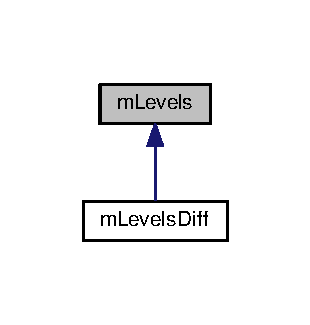
\includegraphics[width=149pt]{struct_k_1_1m_levels__inherit__graph}
\end{center}
\end{figure}
\subsection*{Public Member Functions}
\begin{DoxyCompactItemize}
\item 
\hyperlink{struct_k_1_1m_levels_a99aefce6c3d0d6c9d996bc96f9684e45}{m\+Levels} ()
\item 
\hyperlink{struct_k_1_1m_levels_a10ca86e0fae83aa06fb5943dc4031e1b}{m\+Levels} (vector$<$ \hyperlink{struct_k_1_1m_level}{m\+Level} $>$ b, vector$<$ \hyperlink{struct_k_1_1m_level}{m\+Level} $>$ a)
\item 
\hyperlink{km_8h_a392f9b7f384aa3539bbb890b059f5b8c}{m\+Price} \hyperlink{struct_k_1_1m_levels_a602a1ff7530a970b9f77f20df20d7b8c}{spread} ()
\item 
bool \hyperlink{struct_k_1_1m_levels_a3f37b042a1e7cd4bd38fc564de81f0da}{empty} ()
\end{DoxyCompactItemize}
\subsection*{Data Fields}
\begin{DoxyCompactItemize}
\item 
vector$<$ \hyperlink{struct_k_1_1m_level}{m\+Level} $>$ \hyperlink{struct_k_1_1m_levels_ae01c62df8fdd345c0e9024d06ef863b4}{bids}
\item 
vector$<$ \hyperlink{struct_k_1_1m_level}{m\+Level} $>$ \hyperlink{struct_k_1_1m_levels_a3ba37a921ed6b2dac154fea1798db0d0}{asks}
\end{DoxyCompactItemize}


\subsection{Detailed Description}


Definition at line 548 of file km.\+h.



\subsection{Constructor \& Destructor Documentation}
\index{K\+::m\+Levels@{K\+::m\+Levels}!m\+Levels@{m\+Levels}}
\index{m\+Levels@{m\+Levels}!K\+::m\+Levels@{K\+::m\+Levels}}
\subsubsection[{\texorpdfstring{m\+Levels()}{mLevels()}}]{\setlength{\rightskip}{0pt plus 5cm}{\bf m\+Levels} (
\begin{DoxyParamCaption}
{}
\end{DoxyParamCaption}
)\hspace{0.3cm}{\ttfamily [inline]}}\hypertarget{struct_k_1_1m_levels_a99aefce6c3d0d6c9d996bc96f9684e45}{}\label{struct_k_1_1m_levels_a99aefce6c3d0d6c9d996bc96f9684e45}


Definition at line 551 of file km.\+h.

\index{K\+::m\+Levels@{K\+::m\+Levels}!m\+Levels@{m\+Levels}}
\index{m\+Levels@{m\+Levels}!K\+::m\+Levels@{K\+::m\+Levels}}
\subsubsection[{\texorpdfstring{m\+Levels(vector$<$ m\+Level $>$ b, vector$<$ m\+Level $>$ a)}{mLevels(vector< mLevel > b, vector< mLevel > a)}}]{\setlength{\rightskip}{0pt plus 5cm}{\bf m\+Levels} (
\begin{DoxyParamCaption}
\item[{vector$<$ {\bf m\+Level} $>$}]{b, }
\item[{vector$<$ {\bf m\+Level} $>$}]{a}
\end{DoxyParamCaption}
)\hspace{0.3cm}{\ttfamily [inline]}}\hypertarget{struct_k_1_1m_levels_a10ca86e0fae83aa06fb5943dc4031e1b}{}\label{struct_k_1_1m_levels_a10ca86e0fae83aa06fb5943dc4031e1b}


Definition at line 554 of file km.\+h.



\subsection{Member Function Documentation}
\index{K\+::m\+Levels@{K\+::m\+Levels}!empty@{empty}}
\index{empty@{empty}!K\+::m\+Levels@{K\+::m\+Levels}}
\subsubsection[{\texorpdfstring{empty()}{empty()}}]{\setlength{\rightskip}{0pt plus 5cm}bool empty (
\begin{DoxyParamCaption}
{}
\end{DoxyParamCaption}
)\hspace{0.3cm}{\ttfamily [inline]}}\hypertarget{struct_k_1_1m_levels_a3f37b042a1e7cd4bd38fc564de81f0da}{}\label{struct_k_1_1m_levels_a3f37b042a1e7cd4bd38fc564de81f0da}


Definition at line 560 of file km.\+h.

\index{K\+::m\+Levels@{K\+::m\+Levels}!spread@{spread}}
\index{spread@{spread}!K\+::m\+Levels@{K\+::m\+Levels}}
\subsubsection[{\texorpdfstring{spread()}{spread()}}]{\setlength{\rightskip}{0pt plus 5cm}{\bf m\+Price} spread (
\begin{DoxyParamCaption}
{}
\end{DoxyParamCaption}
)\hspace{0.3cm}{\ttfamily [inline]}}\hypertarget{struct_k_1_1m_levels_a602a1ff7530a970b9f77f20df20d7b8c}{}\label{struct_k_1_1m_levels_a602a1ff7530a970b9f77f20df20d7b8c}


Definition at line 557 of file km.\+h.



\subsection{Field Documentation}
\index{K\+::m\+Levels@{K\+::m\+Levels}!asks@{asks}}
\index{asks@{asks}!K\+::m\+Levels@{K\+::m\+Levels}}
\subsubsection[{\texorpdfstring{asks}{asks}}]{\setlength{\rightskip}{0pt plus 5cm}vector$<${\bf m\+Level}$>$ asks}\hypertarget{struct_k_1_1m_levels_a3ba37a921ed6b2dac154fea1798db0d0}{}\label{struct_k_1_1m_levels_a3ba37a921ed6b2dac154fea1798db0d0}


Definition at line 549 of file km.\+h.

\index{K\+::m\+Levels@{K\+::m\+Levels}!bids@{bids}}
\index{bids@{bids}!K\+::m\+Levels@{K\+::m\+Levels}}
\subsubsection[{\texorpdfstring{bids}{bids}}]{\setlength{\rightskip}{0pt plus 5cm}vector$<${\bf m\+Level}$>$ bids}\hypertarget{struct_k_1_1m_levels_ae01c62df8fdd345c0e9024d06ef863b4}{}\label{struct_k_1_1m_levels_ae01c62df8fdd345c0e9024d06ef863b4}


Definition at line 549 of file km.\+h.



The documentation for this struct was generated from the following file\+:\begin{DoxyCompactItemize}
\item 
\hyperlink{km_8h}{km.\+h}\end{DoxyCompactItemize}

\hypertarget{struct_k_1_1m_levels_diff}{}\section{m\+Levels\+Diff Struct Reference}
\label{struct_k_1_1m_levels_diff}\index{m\+Levels\+Diff@{m\+Levels\+Diff}}


{\ttfamily \#include $<$km.\+h$>$}



Inheritance diagram for m\+Levels\+Diff\+:
\nopagebreak
\begin{figure}[H]
\begin{center}
\leavevmode
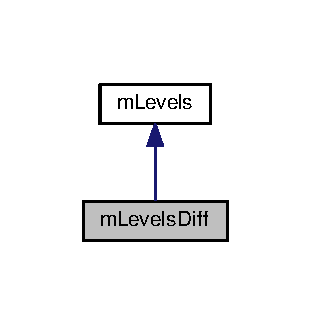
\includegraphics[width=149pt]{struct_k_1_1m_levels_diff__inherit__graph}
\end{center}
\end{figure}


Collaboration diagram for m\+Levels\+Diff\+:
\nopagebreak
\begin{figure}[H]
\begin{center}
\leavevmode
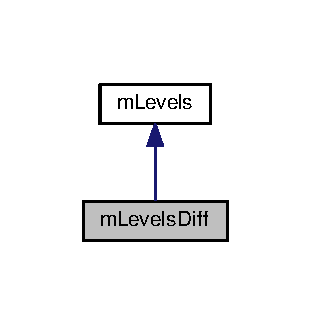
\includegraphics[width=149pt]{struct_k_1_1m_levels_diff__coll__graph}
\end{center}
\end{figure}
\subsection*{Public Member Functions}
\begin{DoxyCompactItemize}
\item 
vector$<$ \hyperlink{struct_k_1_1m_level}{m\+Level} $>$ \hyperlink{struct_k_1_1m_levels_diff_a6fd99c3b5cd57a816d2f91b875644b96}{diff} (const vector$<$ \hyperlink{struct_k_1_1m_level}{m\+Level} $>$ \&from, vector$<$ \hyperlink{struct_k_1_1m_level}{m\+Level} $>$ to)
\item 
json \hyperlink{struct_k_1_1m_levels_diff_a5584a114a1439afa0e01f475c1272e7e}{diff} (const \hyperlink{struct_k_1_1m_levels}{m\+Levels} \&to)
\item 
\hyperlink{struct_k_1_1m_levels}{m\+Levels} \hyperlink{struct_k_1_1m_levels_diff_a8e16cdf30d6439e131fac3807429dec4}{reset} (const \hyperlink{struct_k_1_1m_levels}{m\+Levels} \&from)
\end{DoxyCompactItemize}
\subsection*{Additional Inherited Members}


\subsection{Detailed Description}


Definition at line 570 of file km.\+h.



\subsection{Member Function Documentation}
\index{K\+::m\+Levels\+Diff@{K\+::m\+Levels\+Diff}!diff@{diff}}
\index{diff@{diff}!K\+::m\+Levels\+Diff@{K\+::m\+Levels\+Diff}}
\subsubsection[{\texorpdfstring{diff(const vector$<$ m\+Level $>$ \&from, vector$<$ m\+Level $>$ to)}{diff(const vector< mLevel > &from, vector< mLevel > to)}}]{\setlength{\rightskip}{0pt plus 5cm}vector$<${\bf m\+Level}$>$ diff (
\begin{DoxyParamCaption}
\item[{const vector$<$ {\bf m\+Level} $>$ \&}]{from, }
\item[{vector$<$ {\bf m\+Level} $>$}]{to}
\end{DoxyParamCaption}
)\hspace{0.3cm}{\ttfamily [inline]}}\hypertarget{struct_k_1_1m_levels_diff_a6fd99c3b5cd57a816d2f91b875644b96}{}\label{struct_k_1_1m_levels_diff_a6fd99c3b5cd57a816d2f91b875644b96}


Definition at line 571 of file km.\+h.

\index{K\+::m\+Levels\+Diff@{K\+::m\+Levels\+Diff}!diff@{diff}}
\index{diff@{diff}!K\+::m\+Levels\+Diff@{K\+::m\+Levels\+Diff}}
\subsubsection[{\texorpdfstring{diff(const m\+Levels \&to)}{diff(const mLevels &to)}}]{\setlength{\rightskip}{0pt plus 5cm}json diff (
\begin{DoxyParamCaption}
\item[{const {\bf m\+Levels} \&}]{to}
\end{DoxyParamCaption}
)\hspace{0.3cm}{\ttfamily [inline]}}\hypertarget{struct_k_1_1m_levels_diff_a5584a114a1439afa0e01f475c1272e7e}{}\label{struct_k_1_1m_levels_diff_a5584a114a1439afa0e01f475c1272e7e}


Definition at line 592 of file km.\+h.

\index{K\+::m\+Levels\+Diff@{K\+::m\+Levels\+Diff}!reset@{reset}}
\index{reset@{reset}!K\+::m\+Levels\+Diff@{K\+::m\+Levels\+Diff}}
\subsubsection[{\texorpdfstring{reset(const m\+Levels \&from)}{reset(const mLevels &from)}}]{\setlength{\rightskip}{0pt plus 5cm}{\bf m\+Levels} reset (
\begin{DoxyParamCaption}
\item[{const {\bf m\+Levels} \&}]{from}
\end{DoxyParamCaption}
)\hspace{0.3cm}{\ttfamily [inline]}}\hypertarget{struct_k_1_1m_levels_diff_a8e16cdf30d6439e131fac3807429dec4}{}\label{struct_k_1_1m_levels_diff_a8e16cdf30d6439e131fac3807429dec4}


Definition at line 599 of file km.\+h.



The documentation for this struct was generated from the following file\+:\begin{DoxyCompactItemize}
\item 
\hyperlink{km_8h}{km.\+h}\end{DoxyCompactItemize}

\hypertarget{struct_k_1_1m_order}{}\section{m\+Order Struct Reference}
\label{struct_k_1_1m_order}\index{m\+Order@{m\+Order}}


{\ttfamily \#include $<$km.\+h$>$}



Collaboration diagram for m\+Order\+:
\nopagebreak
\begin{figure}[H]
\begin{center}
\leavevmode
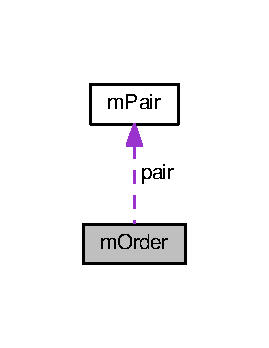
\includegraphics[width=129pt]{struct_k_1_1m_order__coll__graph}
\end{center}
\end{figure}
\subsection*{Public Member Functions}
\begin{DoxyCompactItemize}
\item 
\hyperlink{struct_k_1_1m_order_a6b30d89f1fbef9b56d8e678c49ab225f}{m\+Order} ()
\item 
\hyperlink{struct_k_1_1m_order_a5b7277822fa6487df0498ebc5fecc715}{m\+Order} (\hyperlink{km_8h_a23233b27e494114073abc4d494b05626}{m\+Rand\+Id} o, \hyperlink{namespace_k_a9ca92b450f3b1738c485770d136ac9e0}{m\+Status} s)
\item 
\hyperlink{struct_k_1_1m_order_abc5cbba58af76ee5f1ef93f7eef5a3f0}{m\+Order} (\hyperlink{km_8h_a23233b27e494114073abc4d494b05626}{m\+Rand\+Id} o, \hyperlink{km_8h_a23233b27e494114073abc4d494b05626}{m\+Rand\+Id} e, \hyperlink{namespace_k_a9ca92b450f3b1738c485770d136ac9e0}{m\+Status} s, \hyperlink{km_8h_a392f9b7f384aa3539bbb890b059f5b8c}{m\+Price} p, \hyperlink{km_8h_ad4d00888c55a47a8a40ed8020d176086}{m\+Amount} \hyperlink{namespace_k_a211862d8b09ec46a051464b6859c1306a7694f4a66316e53c8cdd9d9954bd611d}{q}, \hyperlink{km_8h_ad4d00888c55a47a8a40ed8020d176086}{m\+Amount} \hyperlink{namespace_k_a211862d8b09ec46a051464b6859c1306af09564c9ca56850d4cd6b3319e541aee}{Q})
\item 
\hyperlink{struct_k_1_1m_order_a291bbc8e7cb35b53e1ef3885de56c08e}{m\+Order} (\hyperlink{km_8h_a23233b27e494114073abc4d494b05626}{m\+Rand\+Id} o, \hyperlink{struct_k_1_1m_pair}{m\+Pair} P, \hyperlink{namespace_k_a0b7d0fa0ffc9f87da1d6499cbcee7e94}{m\+Side} S, \hyperlink{km_8h_ad4d00888c55a47a8a40ed8020d176086}{m\+Amount} \hyperlink{namespace_k_a211862d8b09ec46a051464b6859c1306a7694f4a66316e53c8cdd9d9954bd611d}{q}, \hyperlink{namespace_k_a131435180aff10fab1bf3da09af62b0d}{m\+Order\+Type} t, bool i, \hyperlink{km_8h_a392f9b7f384aa3539bbb890b059f5b8c}{m\+Price} p, \hyperlink{namespace_k_a290fccb3fc7d447fdbb93a61f6dfba44}{m\+Time\+In\+Force} F, \hyperlink{namespace_k_a9ca92b450f3b1738c485770d136ac9e0}{m\+Status} s, bool O)
\end{DoxyCompactItemize}
\subsection*{Data Fields}
\begin{DoxyCompactItemize}
\item 
\hyperlink{km_8h_a23233b27e494114073abc4d494b05626}{m\+Rand\+Id} \hyperlink{struct_k_1_1m_order_a8588c7c77ae9e996958ee49bc368837a}{order\+Id}
\item 
\hyperlink{km_8h_a23233b27e494114073abc4d494b05626}{m\+Rand\+Id} \hyperlink{struct_k_1_1m_order_a74fdf2701cf5d1c94eb4cca99251668a}{exchange\+Id}
\item 
\hyperlink{struct_k_1_1m_pair}{m\+Pair} \hyperlink{struct_k_1_1m_order_a11dec7b102d6df830347649bfbf35399}{pair}
\item 
\hyperlink{namespace_k_a0b7d0fa0ffc9f87da1d6499cbcee7e94}{m\+Side} \hyperlink{struct_k_1_1m_order_afc5924267a11b19eb2f198a919a12351}{side}
\item 
\hyperlink{km_8h_a392f9b7f384aa3539bbb890b059f5b8c}{m\+Price} \hyperlink{struct_k_1_1m_order_a96d6f95b2441f538965c5d8c1aa32f4e}{price}
\item 
\hyperlink{km_8h_ad4d00888c55a47a8a40ed8020d176086}{m\+Amount} \hyperlink{struct_k_1_1m_order_ab51872d3926e8302926e8ac851dbb158}{quantity}
\item 
\hyperlink{km_8h_ad4d00888c55a47a8a40ed8020d176086}{m\+Amount} \hyperlink{struct_k_1_1m_order_aff1b87a24fb56767cd817854097cf285}{trade\+Quantity}
\item 
\hyperlink{namespace_k_a131435180aff10fab1bf3da09af62b0d}{m\+Order\+Type} \hyperlink{struct_k_1_1m_order_aa62fbff32723469c5aceebe303d5bd3e}{type}
\item 
\hyperlink{namespace_k_a290fccb3fc7d447fdbb93a61f6dfba44}{m\+Time\+In\+Force} \hyperlink{struct_k_1_1m_order_a322c334ae7e885ce9824010ad89c45cc}{time\+In\+Force}
\item 
\hyperlink{namespace_k_a9ca92b450f3b1738c485770d136ac9e0}{m\+Status} \hyperlink{struct_k_1_1m_order_a75b6138814cca75d94e74c3f39a58e2c}{order\+Status}
\item 
bool \hyperlink{struct_k_1_1m_order_ad675049a10e3a8e1c52973272bbea592}{is\+Pong}
\item 
bool \hyperlink{struct_k_1_1m_order_a18806f6d9c3312842bbce443121e0450}{prefer\+Post\+Only}
\item 
\hyperlink{km_8h_ad02a70cba4c52ba2013e5e32ceaeac1c}{m\+Clock} \hyperlink{struct_k_1_1m_order_a8c7be9fac36539b28a92dd5240ec377b}{time}
\item 
\hyperlink{km_8h_ad02a70cba4c52ba2013e5e32ceaeac1c}{m\+Clock} \hyperlink{struct_k_1_1m_order_aa0b6b1a7135bcd07640a190bda611921}{latency}
\item 
\hyperlink{km_8h_ad02a70cba4c52ba2013e5e32ceaeac1c}{m\+Clock} \hyperlink{struct_k_1_1m_order_a078c85c357828219c070420c22e3215a}{\+\_\+waiting\+Cancel}
\end{DoxyCompactItemize}


\subsection{Detailed Description}


Definition at line 475 of file km.\+h.



\subsection{Constructor \& Destructor Documentation}
\index{K\+::m\+Order@{K\+::m\+Order}!m\+Order@{m\+Order}}
\index{m\+Order@{m\+Order}!K\+::m\+Order@{K\+::m\+Order}}
\subsubsection[{\texorpdfstring{m\+Order()}{mOrder()}}]{\setlength{\rightskip}{0pt plus 5cm}{\bf m\+Order} (
\begin{DoxyParamCaption}
{}
\end{DoxyParamCaption}
)\hspace{0.3cm}{\ttfamily [inline]}}\hypertarget{struct_k_1_1m_order_a6b30d89f1fbef9b56d8e678c49ab225f}{}\label{struct_k_1_1m_order_a6b30d89f1fbef9b56d8e678c49ab225f}


Definition at line 491 of file km.\+h.

\index{K\+::m\+Order@{K\+::m\+Order}!m\+Order@{m\+Order}}
\index{m\+Order@{m\+Order}!K\+::m\+Order@{K\+::m\+Order}}
\subsubsection[{\texorpdfstring{m\+Order(m\+Rand\+Id o, m\+Status s)}{mOrder(mRandId o, mStatus s)}}]{\setlength{\rightskip}{0pt plus 5cm}{\bf m\+Order} (
\begin{DoxyParamCaption}
\item[{{\bf m\+Rand\+Id}}]{o, }
\item[{{\bf m\+Status}}]{s}
\end{DoxyParamCaption}
)\hspace{0.3cm}{\ttfamily [inline]}}\hypertarget{struct_k_1_1m_order_a5b7277822fa6487df0498ebc5fecc715}{}\label{struct_k_1_1m_order_a5b7277822fa6487df0498ebc5fecc715}


Definition at line 494 of file km.\+h.

\index{K\+::m\+Order@{K\+::m\+Order}!m\+Order@{m\+Order}}
\index{m\+Order@{m\+Order}!K\+::m\+Order@{K\+::m\+Order}}
\subsubsection[{\texorpdfstring{m\+Order(m\+Rand\+Id o, m\+Rand\+Id e, m\+Status s, m\+Price p, m\+Amount q, m\+Amount Q)}{mOrder(mRandId o, mRandId e, mStatus s, mPrice p, mAmount q, mAmount Q)}}]{\setlength{\rightskip}{0pt plus 5cm}{\bf m\+Order} (
\begin{DoxyParamCaption}
\item[{{\bf m\+Rand\+Id}}]{o, }
\item[{{\bf m\+Rand\+Id}}]{e, }
\item[{{\bf m\+Status}}]{s, }
\item[{{\bf m\+Price}}]{p, }
\item[{{\bf m\+Amount}}]{q, }
\item[{{\bf m\+Amount}}]{Q}
\end{DoxyParamCaption}
)\hspace{0.3cm}{\ttfamily [inline]}}\hypertarget{struct_k_1_1m_order_abc5cbba58af76ee5f1ef93f7eef5a3f0}{}\label{struct_k_1_1m_order_abc5cbba58af76ee5f1ef93f7eef5a3f0}


Definition at line 497 of file km.\+h.

\index{K\+::m\+Order@{K\+::m\+Order}!m\+Order@{m\+Order}}
\index{m\+Order@{m\+Order}!K\+::m\+Order@{K\+::m\+Order}}
\subsubsection[{\texorpdfstring{m\+Order(m\+Rand\+Id o, m\+Pair P, m\+Side S, m\+Amount q, m\+Order\+Type t, bool i, m\+Price p, m\+Time\+In\+Force F, m\+Status s, bool O)}{mOrder(mRandId o, mPair P, mSide S, mAmount q, mOrderType t, bool i, mPrice p, mTimeInForce F, mStatus s, bool O)}}]{\setlength{\rightskip}{0pt plus 5cm}{\bf m\+Order} (
\begin{DoxyParamCaption}
\item[{{\bf m\+Rand\+Id}}]{o, }
\item[{{\bf m\+Pair}}]{P, }
\item[{{\bf m\+Side}}]{S, }
\item[{{\bf m\+Amount}}]{q, }
\item[{{\bf m\+Order\+Type}}]{t, }
\item[{bool}]{i, }
\item[{{\bf m\+Price}}]{p, }
\item[{{\bf m\+Time\+In\+Force}}]{F, }
\item[{{\bf m\+Status}}]{s, }
\item[{bool}]{O}
\end{DoxyParamCaption}
)\hspace{0.3cm}{\ttfamily [inline]}}\hypertarget{struct_k_1_1m_order_a291bbc8e7cb35b53e1ef3885de56c08e}{}\label{struct_k_1_1m_order_a291bbc8e7cb35b53e1ef3885de56c08e}


Definition at line 500 of file km.\+h.



\subsection{Field Documentation}
\index{K\+::m\+Order@{K\+::m\+Order}!\+\_\+waiting\+Cancel@{\+\_\+waiting\+Cancel}}
\index{\+\_\+waiting\+Cancel@{\+\_\+waiting\+Cancel}!K\+::m\+Order@{K\+::m\+Order}}
\subsubsection[{\texorpdfstring{\+\_\+waiting\+Cancel}{_waitingCancel}}]{\setlength{\rightskip}{0pt plus 5cm}{\bf m\+Clock} \+\_\+waiting\+Cancel}\hypertarget{struct_k_1_1m_order_a078c85c357828219c070420c22e3215a}{}\label{struct_k_1_1m_order_a078c85c357828219c070420c22e3215a}


Definition at line 488 of file km.\+h.

\index{K\+::m\+Order@{K\+::m\+Order}!exchange\+Id@{exchange\+Id}}
\index{exchange\+Id@{exchange\+Id}!K\+::m\+Order@{K\+::m\+Order}}
\subsubsection[{\texorpdfstring{exchange\+Id}{exchangeId}}]{\setlength{\rightskip}{0pt plus 5cm}{\bf m\+Rand\+Id} exchange\+Id}\hypertarget{struct_k_1_1m_order_a74fdf2701cf5d1c94eb4cca99251668a}{}\label{struct_k_1_1m_order_a74fdf2701cf5d1c94eb4cca99251668a}


Definition at line 476 of file km.\+h.

\index{K\+::m\+Order@{K\+::m\+Order}!is\+Pong@{is\+Pong}}
\index{is\+Pong@{is\+Pong}!K\+::m\+Order@{K\+::m\+Order}}
\subsubsection[{\texorpdfstring{is\+Pong}{isPong}}]{\setlength{\rightskip}{0pt plus 5cm}bool is\+Pong}\hypertarget{struct_k_1_1m_order_ad675049a10e3a8e1c52973272bbea592}{}\label{struct_k_1_1m_order_ad675049a10e3a8e1c52973272bbea592}


Definition at line 486 of file km.\+h.

\index{K\+::m\+Order@{K\+::m\+Order}!latency@{latency}}
\index{latency@{latency}!K\+::m\+Order@{K\+::m\+Order}}
\subsubsection[{\texorpdfstring{latency}{latency}}]{\setlength{\rightskip}{0pt plus 5cm}{\bf m\+Clock} latency}\hypertarget{struct_k_1_1m_order_aa0b6b1a7135bcd07640a190bda611921}{}\label{struct_k_1_1m_order_aa0b6b1a7135bcd07640a190bda611921}


Definition at line 488 of file km.\+h.

\index{K\+::m\+Order@{K\+::m\+Order}!order\+Id@{order\+Id}}
\index{order\+Id@{order\+Id}!K\+::m\+Order@{K\+::m\+Order}}
\subsubsection[{\texorpdfstring{order\+Id}{orderId}}]{\setlength{\rightskip}{0pt plus 5cm}{\bf m\+Rand\+Id} order\+Id}\hypertarget{struct_k_1_1m_order_a8588c7c77ae9e996958ee49bc368837a}{}\label{struct_k_1_1m_order_a8588c7c77ae9e996958ee49bc368837a}


Definition at line 476 of file km.\+h.

\index{K\+::m\+Order@{K\+::m\+Order}!order\+Status@{order\+Status}}
\index{order\+Status@{order\+Status}!K\+::m\+Order@{K\+::m\+Order}}
\subsubsection[{\texorpdfstring{order\+Status}{orderStatus}}]{\setlength{\rightskip}{0pt plus 5cm}{\bf m\+Status} order\+Status}\hypertarget{struct_k_1_1m_order_a75b6138814cca75d94e74c3f39a58e2c}{}\label{struct_k_1_1m_order_a75b6138814cca75d94e74c3f39a58e2c}


Definition at line 485 of file km.\+h.

\index{K\+::m\+Order@{K\+::m\+Order}!pair@{pair}}
\index{pair@{pair}!K\+::m\+Order@{K\+::m\+Order}}
\subsubsection[{\texorpdfstring{pair}{pair}}]{\setlength{\rightskip}{0pt plus 5cm}{\bf m\+Pair} pair}\hypertarget{struct_k_1_1m_order_a11dec7b102d6df830347649bfbf35399}{}\label{struct_k_1_1m_order_a11dec7b102d6df830347649bfbf35399}


Definition at line 478 of file km.\+h.

\index{K\+::m\+Order@{K\+::m\+Order}!prefer\+Post\+Only@{prefer\+Post\+Only}}
\index{prefer\+Post\+Only@{prefer\+Post\+Only}!K\+::m\+Order@{K\+::m\+Order}}
\subsubsection[{\texorpdfstring{prefer\+Post\+Only}{preferPostOnly}}]{\setlength{\rightskip}{0pt plus 5cm}bool prefer\+Post\+Only}\hypertarget{struct_k_1_1m_order_a18806f6d9c3312842bbce443121e0450}{}\label{struct_k_1_1m_order_a18806f6d9c3312842bbce443121e0450}


Definition at line 486 of file km.\+h.

\index{K\+::m\+Order@{K\+::m\+Order}!price@{price}}
\index{price@{price}!K\+::m\+Order@{K\+::m\+Order}}
\subsubsection[{\texorpdfstring{price}{price}}]{\setlength{\rightskip}{0pt plus 5cm}{\bf m\+Price} price}\hypertarget{struct_k_1_1m_order_a96d6f95b2441f538965c5d8c1aa32f4e}{}\label{struct_k_1_1m_order_a96d6f95b2441f538965c5d8c1aa32f4e}


Definition at line 480 of file km.\+h.

\index{K\+::m\+Order@{K\+::m\+Order}!quantity@{quantity}}
\index{quantity@{quantity}!K\+::m\+Order@{K\+::m\+Order}}
\subsubsection[{\texorpdfstring{quantity}{quantity}}]{\setlength{\rightskip}{0pt plus 5cm}{\bf m\+Amount} quantity}\hypertarget{struct_k_1_1m_order_ab51872d3926e8302926e8ac851dbb158}{}\label{struct_k_1_1m_order_ab51872d3926e8302926e8ac851dbb158}


Definition at line 481 of file km.\+h.

\index{K\+::m\+Order@{K\+::m\+Order}!side@{side}}
\index{side@{side}!K\+::m\+Order@{K\+::m\+Order}}
\subsubsection[{\texorpdfstring{side}{side}}]{\setlength{\rightskip}{0pt plus 5cm}{\bf m\+Side} side}\hypertarget{struct_k_1_1m_order_afc5924267a11b19eb2f198a919a12351}{}\label{struct_k_1_1m_order_afc5924267a11b19eb2f198a919a12351}


Definition at line 479 of file km.\+h.

\index{K\+::m\+Order@{K\+::m\+Order}!time@{time}}
\index{time@{time}!K\+::m\+Order@{K\+::m\+Order}}
\subsubsection[{\texorpdfstring{time}{time}}]{\setlength{\rightskip}{0pt plus 5cm}{\bf m\+Clock} time}\hypertarget{struct_k_1_1m_order_a8c7be9fac36539b28a92dd5240ec377b}{}\label{struct_k_1_1m_order_a8c7be9fac36539b28a92dd5240ec377b}


Definition at line 488 of file km.\+h.

\index{K\+::m\+Order@{K\+::m\+Order}!time\+In\+Force@{time\+In\+Force}}
\index{time\+In\+Force@{time\+In\+Force}!K\+::m\+Order@{K\+::m\+Order}}
\subsubsection[{\texorpdfstring{time\+In\+Force}{timeInForce}}]{\setlength{\rightskip}{0pt plus 5cm}{\bf m\+Time\+In\+Force} time\+In\+Force}\hypertarget{struct_k_1_1m_order_a322c334ae7e885ce9824010ad89c45cc}{}\label{struct_k_1_1m_order_a322c334ae7e885ce9824010ad89c45cc}


Definition at line 484 of file km.\+h.

\index{K\+::m\+Order@{K\+::m\+Order}!trade\+Quantity@{trade\+Quantity}}
\index{trade\+Quantity@{trade\+Quantity}!K\+::m\+Order@{K\+::m\+Order}}
\subsubsection[{\texorpdfstring{trade\+Quantity}{tradeQuantity}}]{\setlength{\rightskip}{0pt plus 5cm}{\bf m\+Amount} trade\+Quantity}\hypertarget{struct_k_1_1m_order_aff1b87a24fb56767cd817854097cf285}{}\label{struct_k_1_1m_order_aff1b87a24fb56767cd817854097cf285}


Definition at line 481 of file km.\+h.

\index{K\+::m\+Order@{K\+::m\+Order}!type@{type}}
\index{type@{type}!K\+::m\+Order@{K\+::m\+Order}}
\subsubsection[{\texorpdfstring{type}{type}}]{\setlength{\rightskip}{0pt plus 5cm}{\bf m\+Order\+Type} type}\hypertarget{struct_k_1_1m_order_aa62fbff32723469c5aceebe303d5bd3e}{}\label{struct_k_1_1m_order_aa62fbff32723469c5aceebe303d5bd3e}


Definition at line 483 of file km.\+h.



The documentation for this struct was generated from the following file\+:\begin{DoxyCompactItemize}
\item 
\hyperlink{km_8h}{km.\+h}\end{DoxyCompactItemize}

\hypertarget{struct_k_1_1m_pair}{}\section{m\+Pair Struct Reference}
\label{struct_k_1_1m_pair}\index{m\+Pair@{m\+Pair}}


{\ttfamily \#include $<$km.\+h$>$}

\subsection*{Public Member Functions}
\begin{DoxyCompactItemize}
\item 
\hyperlink{struct_k_1_1m_pair_a1d94c6e5fb7ac6b74c3b886ef535ad36}{m\+Pair} ()
\item 
\hyperlink{struct_k_1_1m_pair_a9f3d32f3fdf994034c03e8aaa05d58c7}{m\+Pair} (\hyperlink{km_8h_a0299927fb26276a1e0f4c2b4dedb698e}{m\+Coin\+Id} b, \hyperlink{km_8h_a0299927fb26276a1e0f4c2b4dedb698e}{m\+Coin\+Id} \hyperlink{namespace_k_a211862d8b09ec46a051464b6859c1306a7694f4a66316e53c8cdd9d9954bd611d}{q})
\end{DoxyCompactItemize}
\subsection*{Data Fields}
\begin{DoxyCompactItemize}
\item 
\hyperlink{km_8h_a0299927fb26276a1e0f4c2b4dedb698e}{m\+Coin\+Id} \hyperlink{struct_k_1_1m_pair_a88838a75375332fd734e38ba4d7d870c}{base}
\item 
\hyperlink{km_8h_a0299927fb26276a1e0f4c2b4dedb698e}{m\+Coin\+Id} \hyperlink{struct_k_1_1m_pair_abb05d77de0b838cdc580fe5759070aad}{quote}
\end{DoxyCompactItemize}


\subsection{Detailed Description}


Definition at line 251 of file km.\+h.



\subsection{Constructor \& Destructor Documentation}
\index{K\+::m\+Pair@{K\+::m\+Pair}!m\+Pair@{m\+Pair}}
\index{m\+Pair@{m\+Pair}!K\+::m\+Pair@{K\+::m\+Pair}}
\subsubsection[{\texorpdfstring{m\+Pair()}{mPair()}}]{\setlength{\rightskip}{0pt plus 5cm}{\bf m\+Pair} (
\begin{DoxyParamCaption}
{}
\end{DoxyParamCaption}
)\hspace{0.3cm}{\ttfamily [inline]}}\hypertarget{struct_k_1_1m_pair_a1d94c6e5fb7ac6b74c3b886ef535ad36}{}\label{struct_k_1_1m_pair_a1d94c6e5fb7ac6b74c3b886ef535ad36}


Definition at line 254 of file km.\+h.

\index{K\+::m\+Pair@{K\+::m\+Pair}!m\+Pair@{m\+Pair}}
\index{m\+Pair@{m\+Pair}!K\+::m\+Pair@{K\+::m\+Pair}}
\subsubsection[{\texorpdfstring{m\+Pair(m\+Coin\+Id b, m\+Coin\+Id q)}{mPair(mCoinId b, mCoinId q)}}]{\setlength{\rightskip}{0pt plus 5cm}{\bf m\+Pair} (
\begin{DoxyParamCaption}
\item[{{\bf m\+Coin\+Id}}]{b, }
\item[{{\bf m\+Coin\+Id}}]{q}
\end{DoxyParamCaption}
)\hspace{0.3cm}{\ttfamily [inline]}}\hypertarget{struct_k_1_1m_pair_a9f3d32f3fdf994034c03e8aaa05d58c7}{}\label{struct_k_1_1m_pair_a9f3d32f3fdf994034c03e8aaa05d58c7}


Definition at line 257 of file km.\+h.



\subsection{Field Documentation}
\index{K\+::m\+Pair@{K\+::m\+Pair}!base@{base}}
\index{base@{base}!K\+::m\+Pair@{K\+::m\+Pair}}
\subsubsection[{\texorpdfstring{base}{base}}]{\setlength{\rightskip}{0pt plus 5cm}{\bf m\+Coin\+Id} base}\hypertarget{struct_k_1_1m_pair_a88838a75375332fd734e38ba4d7d870c}{}\label{struct_k_1_1m_pair_a88838a75375332fd734e38ba4d7d870c}


Definition at line 252 of file km.\+h.

\index{K\+::m\+Pair@{K\+::m\+Pair}!quote@{quote}}
\index{quote@{quote}!K\+::m\+Pair@{K\+::m\+Pair}}
\subsubsection[{\texorpdfstring{quote}{quote}}]{\setlength{\rightskip}{0pt plus 5cm}{\bf m\+Coin\+Id} quote}\hypertarget{struct_k_1_1m_pair_abb05d77de0b838cdc580fe5759070aad}{}\label{struct_k_1_1m_pair_abb05d77de0b838cdc580fe5759070aad}


Definition at line 252 of file km.\+h.



The documentation for this struct was generated from the following file\+:\begin{DoxyCompactItemize}
\item 
\hyperlink{km_8h}{km.\+h}\end{DoxyCompactItemize}

\hypertarget{struct_k_1_1m_position}{}\section{m\+Position Struct Reference}
\label{struct_k_1_1m_position}\index{m\+Position@{m\+Position}}


{\ttfamily \#include $<$km.\+h$>$}



Collaboration diagram for m\+Position\+:
\nopagebreak
\begin{figure}[H]
\begin{center}
\leavevmode
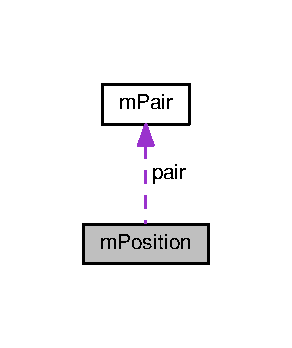
\includegraphics[width=140pt]{struct_k_1_1m_position__coll__graph}
\end{center}
\end{figure}
\subsection*{Public Member Functions}
\begin{DoxyCompactItemize}
\item 
\hyperlink{struct_k_1_1m_position_a31f8f5c2c64206935eeebf00f7017e62}{m\+Position} ()
\item 
\hyperlink{struct_k_1_1m_position_ad6429b29c6410b15083e4b90e5130231}{m\+Position} (\hyperlink{km_8h_ad4d00888c55a47a8a40ed8020d176086}{m\+Amount} bA, \hyperlink{km_8h_ad4d00888c55a47a8a40ed8020d176086}{m\+Amount} qA, \hyperlink{km_8h_ad4d00888c55a47a8a40ed8020d176086}{m\+Amount} q\+AV, \hyperlink{km_8h_ad4d00888c55a47a8a40ed8020d176086}{m\+Amount} bH, \hyperlink{km_8h_ad4d00888c55a47a8a40ed8020d176086}{m\+Amount} qH, \hyperlink{km_8h_ad4d00888c55a47a8a40ed8020d176086}{m\+Amount} bT, \hyperlink{km_8h_ad4d00888c55a47a8a40ed8020d176086}{m\+Amount} qT, \hyperlink{km_8h_ad4d00888c55a47a8a40ed8020d176086}{m\+Amount} bV, \hyperlink{km_8h_ad4d00888c55a47a8a40ed8020d176086}{m\+Amount} qV, \hyperlink{km_8h_ad4d00888c55a47a8a40ed8020d176086}{m\+Amount} bP, \hyperlink{km_8h_ad4d00888c55a47a8a40ed8020d176086}{m\+Amount} qP, \hyperlink{struct_k_1_1m_pair}{m\+Pair} p)
\item 
bool \hyperlink{struct_k_1_1m_position_a3f37b042a1e7cd4bd38fc564de81f0da}{empty} ()
\end{DoxyCompactItemize}
\subsection*{Data Fields}
\begin{DoxyCompactItemize}
\item 
\hyperlink{km_8h_ad4d00888c55a47a8a40ed8020d176086}{m\+Amount} \hyperlink{struct_k_1_1m_position_a54ab63754ed59e0f7167d5b41d320e40}{base\+Amount}
\item 
\hyperlink{km_8h_ad4d00888c55a47a8a40ed8020d176086}{m\+Amount} \hyperlink{struct_k_1_1m_position_acff2752d5a4e300b20b82133fab1f501}{quote\+Amount}
\item 
\hyperlink{km_8h_ad4d00888c55a47a8a40ed8020d176086}{m\+Amount} \hyperlink{struct_k_1_1m_position_a066ad2fbc6cce3f254d147da5255eae7}{\+\_\+quote\+Amount\+Value}
\item 
\hyperlink{km_8h_ad4d00888c55a47a8a40ed8020d176086}{m\+Amount} \hyperlink{struct_k_1_1m_position_ac6175d7078a5d215338188838dba1800}{base\+Held\+Amount}
\item 
\hyperlink{km_8h_ad4d00888c55a47a8a40ed8020d176086}{m\+Amount} \hyperlink{struct_k_1_1m_position_aca53b8b74d1f770cfb029ec8dd3df4d9}{quote\+Held\+Amount}
\item 
\hyperlink{km_8h_ad4d00888c55a47a8a40ed8020d176086}{m\+Amount} \hyperlink{struct_k_1_1m_position_ab965b19b8d97ea6e0f46d38308479a70}{\+\_\+base\+Total}
\item 
\hyperlink{km_8h_ad4d00888c55a47a8a40ed8020d176086}{m\+Amount} \hyperlink{struct_k_1_1m_position_aba337b0148ad9e78db4325d42f9852eb}{\+\_\+quote\+Total}
\item 
\hyperlink{km_8h_ad4d00888c55a47a8a40ed8020d176086}{m\+Amount} \hyperlink{struct_k_1_1m_position_adbb3d8b288708abaf509a644671fb442}{base\+Value}
\item 
\hyperlink{km_8h_ad4d00888c55a47a8a40ed8020d176086}{m\+Amount} \hyperlink{struct_k_1_1m_position_aa18e1bafbe0751bf4ba417df1da264d9}{quote\+Value}
\item 
\hyperlink{km_8h_ad4d00888c55a47a8a40ed8020d176086}{m\+Amount} \hyperlink{struct_k_1_1m_position_ab91bb0250c8c19834e1ffb19c558b706}{profit\+Base}
\item 
\hyperlink{km_8h_ad4d00888c55a47a8a40ed8020d176086}{m\+Amount} \hyperlink{struct_k_1_1m_position_af61cbd1fb2428e9e2ee95e046f8ef327}{profit\+Quote}
\item 
\hyperlink{struct_k_1_1m_pair}{m\+Pair} \hyperlink{struct_k_1_1m_position_a11dec7b102d6df830347649bfbf35399}{pair}
\end{DoxyCompactItemize}


\subsection{Detailed Description}


Definition at line 366 of file km.\+h.



\subsection{Constructor \& Destructor Documentation}
\index{K\+::m\+Position@{K\+::m\+Position}!m\+Position@{m\+Position}}
\index{m\+Position@{m\+Position}!K\+::m\+Position@{K\+::m\+Position}}
\subsubsection[{\texorpdfstring{m\+Position()}{mPosition()}}]{\setlength{\rightskip}{0pt plus 5cm}{\bf m\+Position} (
\begin{DoxyParamCaption}
{}
\end{DoxyParamCaption}
)\hspace{0.3cm}{\ttfamily [inline]}}\hypertarget{struct_k_1_1m_position_a31f8f5c2c64206935eeebf00f7017e62}{}\label{struct_k_1_1m_position_a31f8f5c2c64206935eeebf00f7017e62}


Definition at line 379 of file km.\+h.

\index{K\+::m\+Position@{K\+::m\+Position}!m\+Position@{m\+Position}}
\index{m\+Position@{m\+Position}!K\+::m\+Position@{K\+::m\+Position}}
\subsubsection[{\texorpdfstring{m\+Position(m\+Amount b\+A, m\+Amount q\+A, m\+Amount q\+A\+V, m\+Amount b\+H, m\+Amount q\+H, m\+Amount b\+T, m\+Amount q\+T, m\+Amount b\+V, m\+Amount q\+V, m\+Amount b\+P, m\+Amount q\+P, m\+Pair p)}{mPosition(mAmount bA, mAmount qA, mAmount qAV, mAmount bH, mAmount qH, mAmount bT, mAmount qT, mAmount bV, mAmount qV, mAmount bP, mAmount qP, mPair p)}}]{\setlength{\rightskip}{0pt plus 5cm}{\bf m\+Position} (
\begin{DoxyParamCaption}
\item[{{\bf m\+Amount}}]{bA, }
\item[{{\bf m\+Amount}}]{qA, }
\item[{{\bf m\+Amount}}]{q\+AV, }
\item[{{\bf m\+Amount}}]{bH, }
\item[{{\bf m\+Amount}}]{qH, }
\item[{{\bf m\+Amount}}]{bT, }
\item[{{\bf m\+Amount}}]{qT, }
\item[{{\bf m\+Amount}}]{bV, }
\item[{{\bf m\+Amount}}]{qV, }
\item[{{\bf m\+Amount}}]{bP, }
\item[{{\bf m\+Amount}}]{qP, }
\item[{{\bf m\+Pair}}]{p}
\end{DoxyParamCaption}
)\hspace{0.3cm}{\ttfamily [inline]}}\hypertarget{struct_k_1_1m_position_ad6429b29c6410b15083e4b90e5130231}{}\label{struct_k_1_1m_position_ad6429b29c6410b15083e4b90e5130231}


Definition at line 382 of file km.\+h.



\subsection{Member Function Documentation}
\index{K\+::m\+Position@{K\+::m\+Position}!empty@{empty}}
\index{empty@{empty}!K\+::m\+Position@{K\+::m\+Position}}
\subsubsection[{\texorpdfstring{empty()}{empty()}}]{\setlength{\rightskip}{0pt plus 5cm}bool empty (
\begin{DoxyParamCaption}
{}
\end{DoxyParamCaption}
)\hspace{0.3cm}{\ttfamily [inline]}}\hypertarget{struct_k_1_1m_position_a3f37b042a1e7cd4bd38fc564de81f0da}{}\label{struct_k_1_1m_position_a3f37b042a1e7cd4bd38fc564de81f0da}


Definition at line 392 of file km.\+h.



\subsection{Field Documentation}
\index{K\+::m\+Position@{K\+::m\+Position}!\+\_\+base\+Total@{\+\_\+base\+Total}}
\index{\+\_\+base\+Total@{\+\_\+base\+Total}!K\+::m\+Position@{K\+::m\+Position}}
\subsubsection[{\texorpdfstring{\+\_\+base\+Total}{_baseTotal}}]{\setlength{\rightskip}{0pt plus 5cm}{\bf m\+Amount} \+\_\+base\+Total}\hypertarget{struct_k_1_1m_position_ab965b19b8d97ea6e0f46d38308479a70}{}\label{struct_k_1_1m_position_ab965b19b8d97ea6e0f46d38308479a70}


Definition at line 367 of file km.\+h.

\index{K\+::m\+Position@{K\+::m\+Position}!\+\_\+quote\+Amount\+Value@{\+\_\+quote\+Amount\+Value}}
\index{\+\_\+quote\+Amount\+Value@{\+\_\+quote\+Amount\+Value}!K\+::m\+Position@{K\+::m\+Position}}
\subsubsection[{\texorpdfstring{\+\_\+quote\+Amount\+Value}{_quoteAmountValue}}]{\setlength{\rightskip}{0pt plus 5cm}{\bf m\+Amount} \+\_\+quote\+Amount\+Value}\hypertarget{struct_k_1_1m_position_a066ad2fbc6cce3f254d147da5255eae7}{}\label{struct_k_1_1m_position_a066ad2fbc6cce3f254d147da5255eae7}


Definition at line 367 of file km.\+h.

\index{K\+::m\+Position@{K\+::m\+Position}!\+\_\+quote\+Total@{\+\_\+quote\+Total}}
\index{\+\_\+quote\+Total@{\+\_\+quote\+Total}!K\+::m\+Position@{K\+::m\+Position}}
\subsubsection[{\texorpdfstring{\+\_\+quote\+Total}{_quoteTotal}}]{\setlength{\rightskip}{0pt plus 5cm}{\bf m\+Amount} \+\_\+quote\+Total}\hypertarget{struct_k_1_1m_position_aba337b0148ad9e78db4325d42f9852eb}{}\label{struct_k_1_1m_position_aba337b0148ad9e78db4325d42f9852eb}


Definition at line 367 of file km.\+h.

\index{K\+::m\+Position@{K\+::m\+Position}!base\+Amount@{base\+Amount}}
\index{base\+Amount@{base\+Amount}!K\+::m\+Position@{K\+::m\+Position}}
\subsubsection[{\texorpdfstring{base\+Amount}{baseAmount}}]{\setlength{\rightskip}{0pt plus 5cm}{\bf m\+Amount} base\+Amount}\hypertarget{struct_k_1_1m_position_a54ab63754ed59e0f7167d5b41d320e40}{}\label{struct_k_1_1m_position_a54ab63754ed59e0f7167d5b41d320e40}


Definition at line 367 of file km.\+h.

\index{K\+::m\+Position@{K\+::m\+Position}!base\+Held\+Amount@{base\+Held\+Amount}}
\index{base\+Held\+Amount@{base\+Held\+Amount}!K\+::m\+Position@{K\+::m\+Position}}
\subsubsection[{\texorpdfstring{base\+Held\+Amount}{baseHeldAmount}}]{\setlength{\rightskip}{0pt plus 5cm}{\bf m\+Amount} base\+Held\+Amount}\hypertarget{struct_k_1_1m_position_ac6175d7078a5d215338188838dba1800}{}\label{struct_k_1_1m_position_ac6175d7078a5d215338188838dba1800}


Definition at line 367 of file km.\+h.

\index{K\+::m\+Position@{K\+::m\+Position}!base\+Value@{base\+Value}}
\index{base\+Value@{base\+Value}!K\+::m\+Position@{K\+::m\+Position}}
\subsubsection[{\texorpdfstring{base\+Value}{baseValue}}]{\setlength{\rightskip}{0pt plus 5cm}{\bf m\+Amount} base\+Value}\hypertarget{struct_k_1_1m_position_adbb3d8b288708abaf509a644671fb442}{}\label{struct_k_1_1m_position_adbb3d8b288708abaf509a644671fb442}


Definition at line 367 of file km.\+h.

\index{K\+::m\+Position@{K\+::m\+Position}!pair@{pair}}
\index{pair@{pair}!K\+::m\+Position@{K\+::m\+Position}}
\subsubsection[{\texorpdfstring{pair}{pair}}]{\setlength{\rightskip}{0pt plus 5cm}{\bf m\+Pair} pair}\hypertarget{struct_k_1_1m_position_a11dec7b102d6df830347649bfbf35399}{}\label{struct_k_1_1m_position_a11dec7b102d6df830347649bfbf35399}


Definition at line 378 of file km.\+h.

\index{K\+::m\+Position@{K\+::m\+Position}!profit\+Base@{profit\+Base}}
\index{profit\+Base@{profit\+Base}!K\+::m\+Position@{K\+::m\+Position}}
\subsubsection[{\texorpdfstring{profit\+Base}{profitBase}}]{\setlength{\rightskip}{0pt plus 5cm}{\bf m\+Amount} profit\+Base}\hypertarget{struct_k_1_1m_position_ab91bb0250c8c19834e1ffb19c558b706}{}\label{struct_k_1_1m_position_ab91bb0250c8c19834e1ffb19c558b706}


Definition at line 367 of file km.\+h.

\index{K\+::m\+Position@{K\+::m\+Position}!profit\+Quote@{profit\+Quote}}
\index{profit\+Quote@{profit\+Quote}!K\+::m\+Position@{K\+::m\+Position}}
\subsubsection[{\texorpdfstring{profit\+Quote}{profitQuote}}]{\setlength{\rightskip}{0pt plus 5cm}{\bf m\+Amount} profit\+Quote}\hypertarget{struct_k_1_1m_position_af61cbd1fb2428e9e2ee95e046f8ef327}{}\label{struct_k_1_1m_position_af61cbd1fb2428e9e2ee95e046f8ef327}


Definition at line 367 of file km.\+h.

\index{K\+::m\+Position@{K\+::m\+Position}!quote\+Amount@{quote\+Amount}}
\index{quote\+Amount@{quote\+Amount}!K\+::m\+Position@{K\+::m\+Position}}
\subsubsection[{\texorpdfstring{quote\+Amount}{quoteAmount}}]{\setlength{\rightskip}{0pt plus 5cm}{\bf m\+Amount} quote\+Amount}\hypertarget{struct_k_1_1m_position_acff2752d5a4e300b20b82133fab1f501}{}\label{struct_k_1_1m_position_acff2752d5a4e300b20b82133fab1f501}


Definition at line 367 of file km.\+h.

\index{K\+::m\+Position@{K\+::m\+Position}!quote\+Held\+Amount@{quote\+Held\+Amount}}
\index{quote\+Held\+Amount@{quote\+Held\+Amount}!K\+::m\+Position@{K\+::m\+Position}}
\subsubsection[{\texorpdfstring{quote\+Held\+Amount}{quoteHeldAmount}}]{\setlength{\rightskip}{0pt plus 5cm}{\bf m\+Amount} quote\+Held\+Amount}\hypertarget{struct_k_1_1m_position_aca53b8b74d1f770cfb029ec8dd3df4d9}{}\label{struct_k_1_1m_position_aca53b8b74d1f770cfb029ec8dd3df4d9}


Definition at line 367 of file km.\+h.

\index{K\+::m\+Position@{K\+::m\+Position}!quote\+Value@{quote\+Value}}
\index{quote\+Value@{quote\+Value}!K\+::m\+Position@{K\+::m\+Position}}
\subsubsection[{\texorpdfstring{quote\+Value}{quoteValue}}]{\setlength{\rightskip}{0pt plus 5cm}{\bf m\+Amount} quote\+Value}\hypertarget{struct_k_1_1m_position_aa18e1bafbe0751bf4ba417df1da264d9}{}\label{struct_k_1_1m_position_aa18e1bafbe0751bf4ba417df1da264d9}


Definition at line 367 of file km.\+h.



The documentation for this struct was generated from the following file\+:\begin{DoxyCompactItemize}
\item 
\hyperlink{km_8h}{km.\+h}\end{DoxyCompactItemize}

\hypertarget{struct_k_1_1m_profit}{}\section{m\+Profit Struct Reference}
\label{struct_k_1_1m_profit}\index{m\+Profit@{m\+Profit}}


{\ttfamily \#include $<$km.\+h$>$}

\subsection*{Public Member Functions}
\begin{DoxyCompactItemize}
\item 
\hyperlink{struct_k_1_1m_profit_a28284966ce82412da109fed28a941653}{m\+Profit} ()
\item 
\hyperlink{struct_k_1_1m_profit_abfd09c3c6542a1053b095d446acce138}{m\+Profit} (\hyperlink{km_8h_ad4d00888c55a47a8a40ed8020d176086}{m\+Amount} b, \hyperlink{km_8h_ad4d00888c55a47a8a40ed8020d176086}{m\+Amount} \hyperlink{namespace_k_a211862d8b09ec46a051464b6859c1306a7694f4a66316e53c8cdd9d9954bd611d}{q}, \hyperlink{km_8h_ad02a70cba4c52ba2013e5e32ceaeac1c}{m\+Clock} t)
\end{DoxyCompactItemize}
\subsection*{Data Fields}
\begin{DoxyCompactItemize}
\item 
\hyperlink{km_8h_ad4d00888c55a47a8a40ed8020d176086}{m\+Amount} \hyperlink{struct_k_1_1m_profit_adbb3d8b288708abaf509a644671fb442}{base\+Value}
\item 
\hyperlink{km_8h_ad4d00888c55a47a8a40ed8020d176086}{m\+Amount} \hyperlink{struct_k_1_1m_profit_aa18e1bafbe0751bf4ba417df1da264d9}{quote\+Value}
\item 
\hyperlink{km_8h_ad02a70cba4c52ba2013e5e32ceaeac1c}{m\+Clock} \hyperlink{struct_k_1_1m_profit_a8c7be9fac36539b28a92dd5240ec377b}{time}
\end{DoxyCompactItemize}


\subsection{Detailed Description}


Definition at line 316 of file km.\+h.



\subsection{Constructor \& Destructor Documentation}
\index{K\+::m\+Profit@{K\+::m\+Profit}!m\+Profit@{m\+Profit}}
\index{m\+Profit@{m\+Profit}!K\+::m\+Profit@{K\+::m\+Profit}}
\subsubsection[{\texorpdfstring{m\+Profit()}{mProfit()}}]{\setlength{\rightskip}{0pt plus 5cm}{\bf m\+Profit} (
\begin{DoxyParamCaption}
{}
\end{DoxyParamCaption}
)\hspace{0.3cm}{\ttfamily [inline]}}\hypertarget{struct_k_1_1m_profit_a28284966ce82412da109fed28a941653}{}\label{struct_k_1_1m_profit_a28284966ce82412da109fed28a941653}


Definition at line 320 of file km.\+h.

\index{K\+::m\+Profit@{K\+::m\+Profit}!m\+Profit@{m\+Profit}}
\index{m\+Profit@{m\+Profit}!K\+::m\+Profit@{K\+::m\+Profit}}
\subsubsection[{\texorpdfstring{m\+Profit(m\+Amount b, m\+Amount q, m\+Clock t)}{mProfit(mAmount b, mAmount q, mClock t)}}]{\setlength{\rightskip}{0pt plus 5cm}{\bf m\+Profit} (
\begin{DoxyParamCaption}
\item[{{\bf m\+Amount}}]{b, }
\item[{{\bf m\+Amount}}]{q, }
\item[{{\bf m\+Clock}}]{t}
\end{DoxyParamCaption}
)\hspace{0.3cm}{\ttfamily [inline]}}\hypertarget{struct_k_1_1m_profit_abfd09c3c6542a1053b095d446acce138}{}\label{struct_k_1_1m_profit_abfd09c3c6542a1053b095d446acce138}


Definition at line 323 of file km.\+h.



\subsection{Field Documentation}
\index{K\+::m\+Profit@{K\+::m\+Profit}!base\+Value@{base\+Value}}
\index{base\+Value@{base\+Value}!K\+::m\+Profit@{K\+::m\+Profit}}
\subsubsection[{\texorpdfstring{base\+Value}{baseValue}}]{\setlength{\rightskip}{0pt plus 5cm}{\bf m\+Amount} base\+Value}\hypertarget{struct_k_1_1m_profit_adbb3d8b288708abaf509a644671fb442}{}\label{struct_k_1_1m_profit_adbb3d8b288708abaf509a644671fb442}


Definition at line 317 of file km.\+h.

\index{K\+::m\+Profit@{K\+::m\+Profit}!quote\+Value@{quote\+Value}}
\index{quote\+Value@{quote\+Value}!K\+::m\+Profit@{K\+::m\+Profit}}
\subsubsection[{\texorpdfstring{quote\+Value}{quoteValue}}]{\setlength{\rightskip}{0pt plus 5cm}{\bf m\+Amount} quote\+Value}\hypertarget{struct_k_1_1m_profit_aa18e1bafbe0751bf4ba417df1da264d9}{}\label{struct_k_1_1m_profit_aa18e1bafbe0751bf4ba417df1da264d9}


Definition at line 317 of file km.\+h.

\index{K\+::m\+Profit@{K\+::m\+Profit}!time@{time}}
\index{time@{time}!K\+::m\+Profit@{K\+::m\+Profit}}
\subsubsection[{\texorpdfstring{time}{time}}]{\setlength{\rightskip}{0pt plus 5cm}{\bf m\+Clock} time}\hypertarget{struct_k_1_1m_profit_a8c7be9fac36539b28a92dd5240ec377b}{}\label{struct_k_1_1m_profit_a8c7be9fac36539b28a92dd5240ec377b}


Definition at line 319 of file km.\+h.



The documentation for this struct was generated from the following file\+:\begin{DoxyCompactItemize}
\item 
\hyperlink{km_8h}{km.\+h}\end{DoxyCompactItemize}

\hypertarget{struct_k_1_1m_quote}{}\section{m\+Quote Struct Reference}
\label{struct_k_1_1m_quote}\index{m\+Quote@{m\+Quote}}


{\ttfamily \#include $<$km.\+h$>$}



Collaboration diagram for m\+Quote\+:
\nopagebreak
\begin{figure}[H]
\begin{center}
\leavevmode
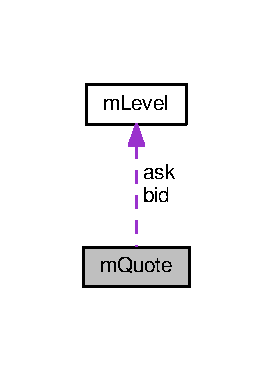
\includegraphics[width=131pt]{struct_k_1_1m_quote__coll__graph}
\end{center}
\end{figure}
\subsection*{Public Member Functions}
\begin{DoxyCompactItemize}
\item 
\hyperlink{struct_k_1_1m_quote_a9d118778e26548c90a1e32280f441f02}{m\+Quote} ()
\item 
\hyperlink{struct_k_1_1m_quote_a32665ec650d6239aeabab46521c8a685}{m\+Quote} (\hyperlink{struct_k_1_1m_level}{m\+Level} b, \hyperlink{struct_k_1_1m_level}{m\+Level} a)
\item 
\hyperlink{struct_k_1_1m_quote_a1ed89b99b3d288cd555223074aca21bd}{m\+Quote} (\hyperlink{struct_k_1_1m_level}{m\+Level} b, \hyperlink{struct_k_1_1m_level}{m\+Level} a, bool bP, bool aP)
\end{DoxyCompactItemize}
\subsection*{Data Fields}
\begin{DoxyCompactItemize}
\item 
\hyperlink{struct_k_1_1m_level}{m\+Level} \hyperlink{struct_k_1_1m_quote_a200a5195c910b871fbfdfd76fcedf05a}{bid}
\item 
\hyperlink{struct_k_1_1m_level}{m\+Level} \hyperlink{struct_k_1_1m_quote_af96a7ede4a006c28cef171f07263e102}{ask}
\item 
bool \hyperlink{struct_k_1_1m_quote_a1c64472cd941ada8dbb3d43fce0c133f}{is\+Bid\+Pong}
\item 
bool \hyperlink{struct_k_1_1m_quote_af8d3a1e2055b25f8560bf9869ce14fe4}{is\+Ask\+Pong}
\end{DoxyCompactItemize}


\subsection{Detailed Description}


Definition at line 612 of file km.\+h.



\subsection{Constructor \& Destructor Documentation}
\index{K\+::m\+Quote@{K\+::m\+Quote}!m\+Quote@{m\+Quote}}
\index{m\+Quote@{m\+Quote}!K\+::m\+Quote@{K\+::m\+Quote}}
\subsubsection[{\texorpdfstring{m\+Quote()}{mQuote()}}]{\setlength{\rightskip}{0pt plus 5cm}{\bf m\+Quote} (
\begin{DoxyParamCaption}
{}
\end{DoxyParamCaption}
)\hspace{0.3cm}{\ttfamily [inline]}}\hypertarget{struct_k_1_1m_quote_a9d118778e26548c90a1e32280f441f02}{}\label{struct_k_1_1m_quote_a9d118778e26548c90a1e32280f441f02}


Definition at line 617 of file km.\+h.

\index{K\+::m\+Quote@{K\+::m\+Quote}!m\+Quote@{m\+Quote}}
\index{m\+Quote@{m\+Quote}!K\+::m\+Quote@{K\+::m\+Quote}}
\subsubsection[{\texorpdfstring{m\+Quote(m\+Level b, m\+Level a)}{mQuote(mLevel b, mLevel a)}}]{\setlength{\rightskip}{0pt plus 5cm}{\bf m\+Quote} (
\begin{DoxyParamCaption}
\item[{{\bf m\+Level}}]{b, }
\item[{{\bf m\+Level}}]{a}
\end{DoxyParamCaption}
)\hspace{0.3cm}{\ttfamily [inline]}}\hypertarget{struct_k_1_1m_quote_a32665ec650d6239aeabab46521c8a685}{}\label{struct_k_1_1m_quote_a32665ec650d6239aeabab46521c8a685}


Definition at line 620 of file km.\+h.

\index{K\+::m\+Quote@{K\+::m\+Quote}!m\+Quote@{m\+Quote}}
\index{m\+Quote@{m\+Quote}!K\+::m\+Quote@{K\+::m\+Quote}}
\subsubsection[{\texorpdfstring{m\+Quote(m\+Level b, m\+Level a, bool b\+P, bool a\+P)}{mQuote(mLevel b, mLevel a, bool bP, bool aP)}}]{\setlength{\rightskip}{0pt plus 5cm}{\bf m\+Quote} (
\begin{DoxyParamCaption}
\item[{{\bf m\+Level}}]{b, }
\item[{{\bf m\+Level}}]{a, }
\item[{bool}]{bP, }
\item[{bool}]{aP}
\end{DoxyParamCaption}
)\hspace{0.3cm}{\ttfamily [inline]}}\hypertarget{struct_k_1_1m_quote_a1ed89b99b3d288cd555223074aca21bd}{}\label{struct_k_1_1m_quote_a1ed89b99b3d288cd555223074aca21bd}


Definition at line 623 of file km.\+h.



\subsection{Field Documentation}
\index{K\+::m\+Quote@{K\+::m\+Quote}!ask@{ask}}
\index{ask@{ask}!K\+::m\+Quote@{K\+::m\+Quote}}
\subsubsection[{\texorpdfstring{ask}{ask}}]{\setlength{\rightskip}{0pt plus 5cm}{\bf m\+Level} ask}\hypertarget{struct_k_1_1m_quote_af96a7ede4a006c28cef171f07263e102}{}\label{struct_k_1_1m_quote_af96a7ede4a006c28cef171f07263e102}


Definition at line 613 of file km.\+h.

\index{K\+::m\+Quote@{K\+::m\+Quote}!bid@{bid}}
\index{bid@{bid}!K\+::m\+Quote@{K\+::m\+Quote}}
\subsubsection[{\texorpdfstring{bid}{bid}}]{\setlength{\rightskip}{0pt plus 5cm}{\bf m\+Level} bid}\hypertarget{struct_k_1_1m_quote_a200a5195c910b871fbfdfd76fcedf05a}{}\label{struct_k_1_1m_quote_a200a5195c910b871fbfdfd76fcedf05a}


Definition at line 613 of file km.\+h.

\index{K\+::m\+Quote@{K\+::m\+Quote}!is\+Ask\+Pong@{is\+Ask\+Pong}}
\index{is\+Ask\+Pong@{is\+Ask\+Pong}!K\+::m\+Quote@{K\+::m\+Quote}}
\subsubsection[{\texorpdfstring{is\+Ask\+Pong}{isAskPong}}]{\setlength{\rightskip}{0pt plus 5cm}bool is\+Ask\+Pong}\hypertarget{struct_k_1_1m_quote_af8d3a1e2055b25f8560bf9869ce14fe4}{}\label{struct_k_1_1m_quote_af8d3a1e2055b25f8560bf9869ce14fe4}


Definition at line 615 of file km.\+h.

\index{K\+::m\+Quote@{K\+::m\+Quote}!is\+Bid\+Pong@{is\+Bid\+Pong}}
\index{is\+Bid\+Pong@{is\+Bid\+Pong}!K\+::m\+Quote@{K\+::m\+Quote}}
\subsubsection[{\texorpdfstring{is\+Bid\+Pong}{isBidPong}}]{\setlength{\rightskip}{0pt plus 5cm}bool is\+Bid\+Pong}\hypertarget{struct_k_1_1m_quote_a1c64472cd941ada8dbb3d43fce0c133f}{}\label{struct_k_1_1m_quote_a1c64472cd941ada8dbb3d43fce0c133f}


Definition at line 615 of file km.\+h.



The documentation for this struct was generated from the following file\+:\begin{DoxyCompactItemize}
\item 
\hyperlink{km_8h}{km.\+h}\end{DoxyCompactItemize}

\hypertarget{struct_k_1_1m_quote_status}{}\section{m\+Quote\+Status Struct Reference}
\label{struct_k_1_1m_quote_status}\index{m\+Quote\+Status@{m\+Quote\+Status}}


{\ttfamily \#include $<$km.\+h$>$}

\subsection*{Public Member Functions}
\begin{DoxyCompactItemize}
\item 
\hyperlink{struct_k_1_1m_quote_status_a0a7505258908838195c0b17cf00bd9f9}{m\+Quote\+Status} ()
\item 
\hyperlink{struct_k_1_1m_quote_status_aed8b89bf13b47ecc96f2e513244d1dfa}{m\+Quote\+Status} (\hyperlink{namespace_k_a76b6774ff9252e574d375a353ecf6736}{m\+Quote\+State} b, \hyperlink{namespace_k_a76b6774ff9252e574d375a353ecf6736}{m\+Quote\+State} a, unsigned int n, unsigned int w, unsigned int d)
\end{DoxyCompactItemize}
\subsection*{Data Fields}
\begin{DoxyCompactItemize}
\item 
\hyperlink{namespace_k_a76b6774ff9252e574d375a353ecf6736}{m\+Quote\+State} \hyperlink{struct_k_1_1m_quote_status_a32c042e88ff93f679a53d90d8c5f0f4a}{bid\+Status}
\item 
\hyperlink{namespace_k_a76b6774ff9252e574d375a353ecf6736}{m\+Quote\+State} \hyperlink{struct_k_1_1m_quote_status_a337d23be0a3a24d260917d7237ab226c}{ask\+Status}
\item 
unsigned int \hyperlink{struct_k_1_1m_quote_status_a28f5330130eff801278c9e5ed7e9d206}{quotes\+In\+Memory\+New}
\item 
unsigned int \hyperlink{struct_k_1_1m_quote_status_a806fde35f6fa8e059f8d35ab6621de2c}{quotes\+In\+Memory\+Working}
\item 
unsigned int \hyperlink{struct_k_1_1m_quote_status_a6aaa53c58be053ff456a485a904539e4}{quotes\+In\+Memory\+Done}
\end{DoxyCompactItemize}


\subsection{Detailed Description}


Definition at line 633 of file km.\+h.



\subsection{Constructor \& Destructor Documentation}
\index{K\+::m\+Quote\+Status@{K\+::m\+Quote\+Status}!m\+Quote\+Status@{m\+Quote\+Status}}
\index{m\+Quote\+Status@{m\+Quote\+Status}!K\+::m\+Quote\+Status@{K\+::m\+Quote\+Status}}
\subsubsection[{\texorpdfstring{m\+Quote\+Status()}{mQuoteStatus()}}]{\setlength{\rightskip}{0pt plus 5cm}{\bf m\+Quote\+Status} (
\begin{DoxyParamCaption}
{}
\end{DoxyParamCaption}
)\hspace{0.3cm}{\ttfamily [inline]}}\hypertarget{struct_k_1_1m_quote_status_a0a7505258908838195c0b17cf00bd9f9}{}\label{struct_k_1_1m_quote_status_a0a7505258908838195c0b17cf00bd9f9}


Definition at line 639 of file km.\+h.

\index{K\+::m\+Quote\+Status@{K\+::m\+Quote\+Status}!m\+Quote\+Status@{m\+Quote\+Status}}
\index{m\+Quote\+Status@{m\+Quote\+Status}!K\+::m\+Quote\+Status@{K\+::m\+Quote\+Status}}
\subsubsection[{\texorpdfstring{m\+Quote\+Status(m\+Quote\+State b, m\+Quote\+State a, unsigned int n, unsigned int w, unsigned int d)}{mQuoteStatus(mQuoteState b, mQuoteState a, unsigned int n, unsigned int w, unsigned int d)}}]{\setlength{\rightskip}{0pt plus 5cm}{\bf m\+Quote\+Status} (
\begin{DoxyParamCaption}
\item[{{\bf m\+Quote\+State}}]{b, }
\item[{{\bf m\+Quote\+State}}]{a, }
\item[{unsigned int}]{n, }
\item[{unsigned int}]{w, }
\item[{unsigned int}]{d}
\end{DoxyParamCaption}
)\hspace{0.3cm}{\ttfamily [inline]}}\hypertarget{struct_k_1_1m_quote_status_aed8b89bf13b47ecc96f2e513244d1dfa}{}\label{struct_k_1_1m_quote_status_aed8b89bf13b47ecc96f2e513244d1dfa}


Definition at line 642 of file km.\+h.



\subsection{Field Documentation}
\index{K\+::m\+Quote\+Status@{K\+::m\+Quote\+Status}!ask\+Status@{ask\+Status}}
\index{ask\+Status@{ask\+Status}!K\+::m\+Quote\+Status@{K\+::m\+Quote\+Status}}
\subsubsection[{\texorpdfstring{ask\+Status}{askStatus}}]{\setlength{\rightskip}{0pt plus 5cm}{\bf m\+Quote\+State} ask\+Status}\hypertarget{struct_k_1_1m_quote_status_a337d23be0a3a24d260917d7237ab226c}{}\label{struct_k_1_1m_quote_status_a337d23be0a3a24d260917d7237ab226c}


Definition at line 634 of file km.\+h.

\index{K\+::m\+Quote\+Status@{K\+::m\+Quote\+Status}!bid\+Status@{bid\+Status}}
\index{bid\+Status@{bid\+Status}!K\+::m\+Quote\+Status@{K\+::m\+Quote\+Status}}
\subsubsection[{\texorpdfstring{bid\+Status}{bidStatus}}]{\setlength{\rightskip}{0pt plus 5cm}{\bf m\+Quote\+State} bid\+Status}\hypertarget{struct_k_1_1m_quote_status_a32c042e88ff93f679a53d90d8c5f0f4a}{}\label{struct_k_1_1m_quote_status_a32c042e88ff93f679a53d90d8c5f0f4a}


Definition at line 634 of file km.\+h.

\index{K\+::m\+Quote\+Status@{K\+::m\+Quote\+Status}!quotes\+In\+Memory\+Done@{quotes\+In\+Memory\+Done}}
\index{quotes\+In\+Memory\+Done@{quotes\+In\+Memory\+Done}!K\+::m\+Quote\+Status@{K\+::m\+Quote\+Status}}
\subsubsection[{\texorpdfstring{quotes\+In\+Memory\+Done}{quotesInMemoryDone}}]{\setlength{\rightskip}{0pt plus 5cm}unsigned int quotes\+In\+Memory\+Done}\hypertarget{struct_k_1_1m_quote_status_a6aaa53c58be053ff456a485a904539e4}{}\label{struct_k_1_1m_quote_status_a6aaa53c58be053ff456a485a904539e4}


Definition at line 636 of file km.\+h.

\index{K\+::m\+Quote\+Status@{K\+::m\+Quote\+Status}!quotes\+In\+Memory\+New@{quotes\+In\+Memory\+New}}
\index{quotes\+In\+Memory\+New@{quotes\+In\+Memory\+New}!K\+::m\+Quote\+Status@{K\+::m\+Quote\+Status}}
\subsubsection[{\texorpdfstring{quotes\+In\+Memory\+New}{quotesInMemoryNew}}]{\setlength{\rightskip}{0pt plus 5cm}unsigned int quotes\+In\+Memory\+New}\hypertarget{struct_k_1_1m_quote_status_a28f5330130eff801278c9e5ed7e9d206}{}\label{struct_k_1_1m_quote_status_a28f5330130eff801278c9e5ed7e9d206}


Definition at line 636 of file km.\+h.

\index{K\+::m\+Quote\+Status@{K\+::m\+Quote\+Status}!quotes\+In\+Memory\+Working@{quotes\+In\+Memory\+Working}}
\index{quotes\+In\+Memory\+Working@{quotes\+In\+Memory\+Working}!K\+::m\+Quote\+Status@{K\+::m\+Quote\+Status}}
\subsubsection[{\texorpdfstring{quotes\+In\+Memory\+Working}{quotesInMemoryWorking}}]{\setlength{\rightskip}{0pt plus 5cm}unsigned int quotes\+In\+Memory\+Working}\hypertarget{struct_k_1_1m_quote_status_a806fde35f6fa8e059f8d35ab6621de2c}{}\label{struct_k_1_1m_quote_status_a806fde35f6fa8e059f8d35ab6621de2c}


Definition at line 636 of file km.\+h.



The documentation for this struct was generated from the following file\+:\begin{DoxyCompactItemize}
\item 
\hyperlink{km_8h}{km.\+h}\end{DoxyCompactItemize}

\hypertarget{struct_k_1_1m_quoting_params}{}\section{m\+Quoting\+Params Struct Reference}
\label{struct_k_1_1m_quoting_params}\index{m\+Quoting\+Params@{m\+Quoting\+Params}}


{\ttfamily \#include $<$km.\+h$>$}

\subsection*{Public Member Functions}
\begin{DoxyCompactItemize}
\item 
void \hyperlink{struct_k_1_1m_quoting_params_a5b3c419df4060973d19148fe5f75b275}{tidy} ()
\item 
void \hyperlink{struct_k_1_1m_quoting_params_a9897581e5bf85e3b75d7159f0621740f}{flag} ()
\item 
void \hyperlink{struct_k_1_1m_quoting_params_a342922b70b5ffb7b8b92b9b9ec1d9ee5}{diff} (\hyperlink{struct_k_1_1m_quoting_params}{m\+Quoting\+Params} \&prev)
\item 
void \hyperlink{struct_k_1_1m_quoting_params_a049d4509d364db17f6654111e95ad64b}{equal} (\hyperlink{struct_k_1_1m_quoting_params}{m\+Quoting\+Params} \&prev)
\end{DoxyCompactItemize}
\subsection*{Data Fields}
\begin{DoxyCompactItemize}
\item 
\hyperlink{km_8h_a392f9b7f384aa3539bbb890b059f5b8c}{m\+Price} \hyperlink{struct_k_1_1m_quoting_params_a4279c166f3d233d69f15f23174b015f5}{width\+Ping} = 2.\+0
\item 
double \hyperlink{struct_k_1_1m_quoting_params_ae713d32ed4985ea64a75a3b67ed2e4d9}{width\+Ping\+Percentage} = 0.\+25
\item 
\hyperlink{km_8h_a392f9b7f384aa3539bbb890b059f5b8c}{m\+Price} \hyperlink{struct_k_1_1m_quoting_params_a259c285d2a55a58a4c5e87f58e18765d}{width\+Pong} = 2.\+0
\item 
double \hyperlink{struct_k_1_1m_quoting_params_acff9ae46960bbd2d759586223fa57081}{width\+Pong\+Percentage} = 0.\+25
\item 
bool \hyperlink{struct_k_1_1m_quoting_params_a3e872a1d8d93fd696268d8abacb97736}{width\+Percentage} = false
\item 
bool \hyperlink{struct_k_1_1m_quoting_params_a7e744b13bec19c083103e7ae84845427}{best\+Width} = true
\item 
\hyperlink{km_8h_ad4d00888c55a47a8a40ed8020d176086}{m\+Amount} \hyperlink{struct_k_1_1m_quoting_params_a78713a07cb23439e664a091f740fef1f}{buy\+Size} = 0.\+02
\item 
unsigned int \hyperlink{struct_k_1_1m_quoting_params_aefdf7026d73172dbed3231b219385e4b}{buy\+Size\+Percentage} = 7
\item 
bool \hyperlink{struct_k_1_1m_quoting_params_a9430749d47750fa7a3571e69aa421524}{buy\+Size\+Max} = false
\item 
\hyperlink{km_8h_ad4d00888c55a47a8a40ed8020d176086}{m\+Amount} \hyperlink{struct_k_1_1m_quoting_params_a4f82c0df812be2c3dc86ab0778b171d7}{sell\+Size} = 0.\+01
\item 
unsigned int \hyperlink{struct_k_1_1m_quoting_params_af5250a47f1886c3ec8366e6c0743434d}{sell\+Size\+Percentage} = 7
\item 
bool \hyperlink{struct_k_1_1m_quoting_params_a91e84c2561413850c96212769eff466c}{sell\+Size\+Max} = false
\item 
\hyperlink{namespace_k_a9d7dedf4873c0cda3ab0c919395b667c}{m\+Ping\+At} \hyperlink{struct_k_1_1m_quoting_params_afb778f21e472d73bf86c2cf855cd4720}{ping\+At} = \hyperlink{namespace_k_a9d7dedf4873c0cda3ab0c919395b667cad20455e0ed8edbd95fbbb7dff3d61503}{m\+Ping\+At\+::\+Both\+Sides}
\item 
\hyperlink{namespace_k_a6bd1ffa01a02e9cf1302f02774ba013f}{m\+Pong\+At} \hyperlink{struct_k_1_1m_quoting_params_aa1a0a930fab278ae84dba744b9df2346}{pong\+At} = \hyperlink{namespace_k_a6bd1ffa01a02e9cf1302f02774ba013fa102eaf65c3a5f9be2898b918b50c0a09}{m\+Pong\+At\+::\+Short\+Ping\+Fair}
\item 
\hyperlink{namespace_k_aad47eca41d4abcf27209f4b673e7b9e9}{m\+Quoting\+Mode} \hyperlink{struct_k_1_1m_quoting_params_aba9219e91199409f90646b018b900dc6}{mode} = \hyperlink{namespace_k_aad47eca41d4abcf27209f4b673e7b9e9aa4ffdcf0dc1f31b9acaf295d75b51d00}{m\+Quoting\+Mode\+::\+Top}
\item 
\hyperlink{namespace_k_a89330b32d78089edeaa5bc6fe48d605d}{m\+Quoting\+Safety} \hyperlink{struct_k_1_1m_quoting_params_a366be3c92bc258600ccf2d6e93cdd852}{safety} = \hyperlink{namespace_k_a89330b32d78089edeaa5bc6fe48d605da8c9d96b1ef82662dd41a42e8528876b6}{m\+Quoting\+Safety\+::\+Boomerang}
\item 
unsigned int \hyperlink{struct_k_1_1m_quoting_params_a66918388a988312b129d487b71d79136}{bullets} = 2
\item 
\hyperlink{km_8h_a392f9b7f384aa3539bbb890b059f5b8c}{m\+Price} \hyperlink{struct_k_1_1m_quoting_params_a682b5a36477fe4df067e2d6f573e98d8}{range} = 0.\+5
\item 
double \hyperlink{struct_k_1_1m_quoting_params_af8622c6c49ec64f7e1ca24ad14b378e6}{range\+Percentage} = 5.\+0
\item 
\hyperlink{namespace_k_ae4a47201f2511ecc8ab5b412e872b9dd}{m\+Fair\+Value\+Model} \hyperlink{struct_k_1_1m_quoting_params_af91dea72c9736ae247e270dcdd166d30}{fv\+Model} = \hyperlink{namespace_k_ae4a47201f2511ecc8ab5b412e872b9dda2a723053ab15920e0c2ecd25a2ede6f9}{m\+Fair\+Value\+Model\+::\+B\+BO}
\item 
\hyperlink{km_8h_ad4d00888c55a47a8a40ed8020d176086}{m\+Amount} \hyperlink{struct_k_1_1m_quoting_params_a41f7e688e22528d01be7373457b533c0}{target\+Base\+Position} = 1.\+0
\item 
unsigned int \hyperlink{struct_k_1_1m_quoting_params_ae7a7b8af9caac8e6704751916b481c87}{target\+Base\+Position\+Percentage} = 50
\item 
\hyperlink{km_8h_ad4d00888c55a47a8a40ed8020d176086}{m\+Amount} \hyperlink{struct_k_1_1m_quoting_params_a158e860ce785d482b11cf81a6544cbd6}{position\+Divergence} = 0.\+9
\item 
\hyperlink{km_8h_ad4d00888c55a47a8a40ed8020d176086}{m\+Amount} \hyperlink{struct_k_1_1m_quoting_params_aad5a5a67d31446bdd70bbaa464080eff}{position\+Divergence\+Min} = 0.\+4
\item 
unsigned int \hyperlink{struct_k_1_1m_quoting_params_a87100c1d4acfed663be3c8a52ac3a646}{position\+Divergence\+Percentage} = 21
\item 
unsigned int \hyperlink{struct_k_1_1m_quoting_params_ac6a1449dd763064f3e4f741db7826f34}{position\+Divergence\+Percentage\+Min} = 10
\item 
\hyperlink{namespace_k_ac928319d6f2b7d9709cd3ca9fa6cb5a7}{m\+P\+Div\+Mode} \hyperlink{struct_k_1_1m_quoting_params_a2304a83d8a52934be7c132f9fb6fd479}{position\+Divergence\+Mode} = \hyperlink{namespace_k_a8708a45c314b4d4bb9e7221009ccee8aae1ba155a9f2e8c3be94020eef32a0301}{m\+P\+Div\+Mode\+::\+Manual}
\item 
bool \hyperlink{struct_k_1_1m_quoting_params_ac8404ecb555d84d2bef12ffae8b401b6}{percentage\+Values} = false
\item 
\hyperlink{namespace_k_a8708a45c314b4d4bb9e7221009ccee8a}{m\+Auto\+Position\+Mode} \hyperlink{struct_k_1_1m_quoting_params_a57aeb3184bd7e2fa299e62ddd0e64273}{auto\+Position\+Mode} = \hyperlink{namespace_k_a8708a45c314b4d4bb9e7221009ccee8aab539e10bdc606700e99b1e0cff611765}{m\+Auto\+Position\+Mode\+::\+E\+W\+M\+A\+\_\+\+LS}
\item 
\hyperlink{namespace_k_a8fb2f5e34d77eef380ac27a7737a3a25}{m\+A\+PR} \hyperlink{struct_k_1_1m_quoting_params_abce7d5d8bfe5b74771f69e8371ad8fb6}{aggressive\+Position\+Rebalancing} = \hyperlink{namespace_k_a89330b32d78089edeaa5bc6fe48d605dad15305d7a4e34e02489c74a5ef542f36}{m\+A\+P\+R\+::\+Off}
\item 
\hyperlink{namespace_k_a2f7964509b276df1811f64989ee56ca5}{m\+S\+OP} \hyperlink{struct_k_1_1m_quoting_params_a827aff7828ab29643db30a5b6e0cafbd}{super\+Trades} = \hyperlink{namespace_k_a89330b32d78089edeaa5bc6fe48d605dad15305d7a4e34e02489c74a5ef542f36}{m\+S\+O\+P\+::\+Off}
\item 
double \hyperlink{struct_k_1_1m_quoting_params_a4220b937e549b61ffd570c9e673ea8a8}{trades\+Per\+Minute} = 0.\+9
\item 
unsigned int \hyperlink{struct_k_1_1m_quoting_params_a0ba45eb10ad95fea001ee29ae4fd5272}{trade\+Rate\+Seconds} = 3
\item 
bool \hyperlink{struct_k_1_1m_quoting_params_a066245465781f4f53120fc1ac38285c9}{protection\+Ewma\+Width\+Ping} = false
\item 
bool \hyperlink{struct_k_1_1m_quoting_params_a3df2bee8175846c2af077d3240f3d269}{protection\+Ewma\+Quote\+Price} = true
\item 
unsigned int \hyperlink{struct_k_1_1m_quoting_params_a8bf870ca98614079b091ef0123b86eab}{protection\+Ewma\+Periods} = 200
\item 
\hyperlink{namespace_k_a648db17031757556a30a6ba51a9ce636}{m\+S\+T\+D\+EV} \hyperlink{struct_k_1_1m_quoting_params_ac799b2adc766e961b812d1a97d97063c}{quoting\+Stdev\+Protection} = \hyperlink{namespace_k_a89330b32d78089edeaa5bc6fe48d605dad15305d7a4e34e02489c74a5ef542f36}{m\+S\+T\+D\+E\+V\+::\+Off}
\item 
bool \hyperlink{struct_k_1_1m_quoting_params_aa0fa38752190501ff21345250e62a843}{quoting\+Stdev\+Bollinger\+Bands} = false
\item 
double \hyperlink{struct_k_1_1m_quoting_params_ac560879d917a01a352c44d54cc9cbadb}{quoting\+Stdev\+Protection\+Factor} = 1.\+0
\item 
unsigned int \hyperlink{struct_k_1_1m_quoting_params_ad94d984ac4098971a3d44ce736edefb0}{quoting\+Stdev\+Protection\+Periods} = 1200
\item 
double \hyperlink{struct_k_1_1m_quoting_params_aa9c1573602f4339de74409d7a69de26f}{ewma\+Sensiblity\+Percentage} = 0.\+5
\item 
bool \hyperlink{struct_k_1_1m_quoting_params_a61b6dfbdc7421efd1a7a7fa36c127ffb}{quoting\+Ewma\+Trend\+Protection} = false
\item 
double \hyperlink{struct_k_1_1m_quoting_params_a14356d95d1c4c6a1c0cfadd22ffbfe3e}{quoting\+Ewma\+Trend\+Threshold} = 2.\+0
\item 
unsigned int \hyperlink{struct_k_1_1m_quoting_params_af296a51a25b34f662a36db31a4481702}{very\+Long\+Ewma\+Periods} = 400
\item 
unsigned int \hyperlink{struct_k_1_1m_quoting_params_a1f51ec10f77d37f7af33d3dc5161b440}{long\+Ewma\+Periods} = 200
\item 
unsigned int \hyperlink{struct_k_1_1m_quoting_params_af0d97776d733257c7f697f39d80962d9}{medium\+Ewma\+Periods} = 100
\item 
unsigned int \hyperlink{struct_k_1_1m_quoting_params_a65a5668435d92d42e7f593610c631d05}{short\+Ewma\+Periods} = 50
\item 
unsigned int \hyperlink{struct_k_1_1m_quoting_params_a9e3ade82ef85cb29dfb6f493b64df9f7}{extra\+Short\+Ewma\+Periods} = 12
\item 
unsigned int \hyperlink{struct_k_1_1m_quoting_params_a6eb0a78fa24178b92665467314fd1b1d}{ultra\+Short\+Ewma\+Periods} = 3
\item 
double \hyperlink{struct_k_1_1m_quoting_params_a66807d8fce3feefad4ba68f020d50bf5}{apr\+Multiplier} = 2
\item 
double \hyperlink{struct_k_1_1m_quoting_params_a48109b838d1faaf4dbe97fe214a6e266}{sop\+Width\+Multiplier} = 2
\item 
double \hyperlink{struct_k_1_1m_quoting_params_a12996d4a63f260eadde561945f4de34a}{sop\+Size\+Multiplier} = 2
\item 
double \hyperlink{struct_k_1_1m_quoting_params_a2f287785df6177addf95607799ab4092}{sop\+Trades\+Multiplier} = 2
\item 
bool \hyperlink{struct_k_1_1m_quoting_params_a3a10c4191849a5c68d4c4837267d184c}{cancel\+Orders\+Auto} = false
\item 
double \hyperlink{struct_k_1_1m_quoting_params_a4b0a67a03f8ad8c612e57f550b026df3}{clean\+Pongs\+Auto} = 0.\+0
\item 
double \hyperlink{struct_k_1_1m_quoting_params_aca375dffd0084ba4ca88fcdfeff7f99c}{profit\+Hour\+Interval} = 0.\+5
\item 
bool \hyperlink{struct_k_1_1m_quoting_params_ac76cbef55dea9f125b6f88259693e97a}{audio} = false
\item 
unsigned int \hyperlink{struct_k_1_1m_quoting_params_a6c5f9f2975a817fbeb1c63a355108658}{delay\+UI} = 7
\item 
bool \hyperlink{struct_k_1_1m_quoting_params_a61446b4fb2c9d0703a4d2de65887792b}{\+\_\+match\+Pings} = true
\item 
bool \hyperlink{struct_k_1_1m_quoting_params_a0e836fed07704cb606e8ba0aaba6ea78}{\+\_\+diff\+V\+L\+EP} = false
\item 
bool \hyperlink{struct_k_1_1m_quoting_params_a1ce33c761bbda9cfde895b9be3c0bef1}{\+\_\+diff\+L\+EP} = false
\item 
bool \hyperlink{struct_k_1_1m_quoting_params_a2b3c89468dc78a966b83f64a7f653833}{\+\_\+diff\+M\+EP} = false
\item 
bool \hyperlink{struct_k_1_1m_quoting_params_a717403a01ee09fe008bd2e69565634c5}{\+\_\+diff\+S\+EP} = false
\item 
bool \hyperlink{struct_k_1_1m_quoting_params_ab502ee083f9bfede1b43659973f9ddcd}{\+\_\+diff\+X\+S\+EP} = false
\item 
bool \hyperlink{struct_k_1_1m_quoting_params_a3742efc61363ad9e1157430da409aa0e}{\+\_\+diff\+U\+EP} = false
\item 
function$<$ void()$>$ $\ast$ \hyperlink{struct_k_1_1m_quoting_params_aeada466ca69f4000ae2121f2c75fa7c6}{calc\+Quote\+After\+Saved\+Params} = nullptr
\end{DoxyCompactItemize}


\subsection{Detailed Description}


Definition at line 41 of file km.\+h.



\subsection{Member Function Documentation}
\index{K\+::m\+Quoting\+Params@{K\+::m\+Quoting\+Params}!diff@{diff}}
\index{diff@{diff}!K\+::m\+Quoting\+Params@{K\+::m\+Quoting\+Params}}
\subsubsection[{\texorpdfstring{diff(m\+Quoting\+Params \&prev)}{diff(mQuotingParams &prev)}}]{\setlength{\rightskip}{0pt plus 5cm}void diff (
\begin{DoxyParamCaption}
\item[{{\bf m\+Quoting\+Params} \&}]{prev}
\end{DoxyParamCaption}
)\hspace{0.3cm}{\ttfamily [inline]}}\hypertarget{struct_k_1_1m_quoting_params_a342922b70b5ffb7b8b92b9b9ec1d9ee5}{}\label{struct_k_1_1m_quoting_params_a342922b70b5ffb7b8b92b9b9ec1d9ee5}


Definition at line 113 of file km.\+h.

\index{K\+::m\+Quoting\+Params@{K\+::m\+Quoting\+Params}!equal@{equal}}
\index{equal@{equal}!K\+::m\+Quoting\+Params@{K\+::m\+Quoting\+Params}}
\subsubsection[{\texorpdfstring{equal(m\+Quoting\+Params \&prev)}{equal(mQuotingParams &prev)}}]{\setlength{\rightskip}{0pt plus 5cm}void equal (
\begin{DoxyParamCaption}
\item[{{\bf m\+Quoting\+Params} \&}]{prev}
\end{DoxyParamCaption}
)\hspace{0.3cm}{\ttfamily [inline]}}\hypertarget{struct_k_1_1m_quoting_params_a049d4509d364db17f6654111e95ad64b}{}\label{struct_k_1_1m_quoting_params_a049d4509d364db17f6654111e95ad64b}


Definition at line 122 of file km.\+h.

\index{K\+::m\+Quoting\+Params@{K\+::m\+Quoting\+Params}!flag@{flag}}
\index{flag@{flag}!K\+::m\+Quoting\+Params@{K\+::m\+Quoting\+Params}}
\subsubsection[{\texorpdfstring{flag()}{flag()}}]{\setlength{\rightskip}{0pt plus 5cm}void flag (
\begin{DoxyParamCaption}
{}
\end{DoxyParamCaption}
)\hspace{0.3cm}{\ttfamily [inline]}}\hypertarget{struct_k_1_1m_quoting_params_a9897581e5bf85e3b75d7159f0621740f}{}\label{struct_k_1_1m_quoting_params_a9897581e5bf85e3b75d7159f0621740f}


Definition at line 110 of file km.\+h.

\index{K\+::m\+Quoting\+Params@{K\+::m\+Quoting\+Params}!tidy@{tidy}}
\index{tidy@{tidy}!K\+::m\+Quoting\+Params@{K\+::m\+Quoting\+Params}}
\subsubsection[{\texorpdfstring{tidy()}{tidy()}}]{\setlength{\rightskip}{0pt plus 5cm}void tidy (
\begin{DoxyParamCaption}
{}
\end{DoxyParamCaption}
)\hspace{0.3cm}{\ttfamily [inline]}}\hypertarget{struct_k_1_1m_quoting_params_a5b3c419df4060973d19148fe5f75b275}{}\label{struct_k_1_1m_quoting_params_a5b3c419df4060973d19148fe5f75b275}


Definition at line 107 of file km.\+h.



\subsection{Field Documentation}
\index{K\+::m\+Quoting\+Params@{K\+::m\+Quoting\+Params}!\+\_\+diff\+L\+EP@{\+\_\+diff\+L\+EP}}
\index{\+\_\+diff\+L\+EP@{\+\_\+diff\+L\+EP}!K\+::m\+Quoting\+Params@{K\+::m\+Quoting\+Params}}
\subsubsection[{\texorpdfstring{\+\_\+diff\+L\+EP}{_diffLEP}}]{\setlength{\rightskip}{0pt plus 5cm}bool \+\_\+diff\+L\+EP = false}\hypertarget{struct_k_1_1m_quoting_params_a1ce33c761bbda9cfde895b9be3c0bef1}{}\label{struct_k_1_1m_quoting_params_a1ce33c761bbda9cfde895b9be3c0bef1}


Definition at line 102 of file km.\+h.

\index{K\+::m\+Quoting\+Params@{K\+::m\+Quoting\+Params}!\+\_\+diff\+M\+EP@{\+\_\+diff\+M\+EP}}
\index{\+\_\+diff\+M\+EP@{\+\_\+diff\+M\+EP}!K\+::m\+Quoting\+Params@{K\+::m\+Quoting\+Params}}
\subsubsection[{\texorpdfstring{\+\_\+diff\+M\+EP}{_diffMEP}}]{\setlength{\rightskip}{0pt plus 5cm}bool \+\_\+diff\+M\+EP = false}\hypertarget{struct_k_1_1m_quoting_params_a2b3c89468dc78a966b83f64a7f653833}{}\label{struct_k_1_1m_quoting_params_a2b3c89468dc78a966b83f64a7f653833}


Definition at line 103 of file km.\+h.

\index{K\+::m\+Quoting\+Params@{K\+::m\+Quoting\+Params}!\+\_\+diff\+S\+EP@{\+\_\+diff\+S\+EP}}
\index{\+\_\+diff\+S\+EP@{\+\_\+diff\+S\+EP}!K\+::m\+Quoting\+Params@{K\+::m\+Quoting\+Params}}
\subsubsection[{\texorpdfstring{\+\_\+diff\+S\+EP}{_diffSEP}}]{\setlength{\rightskip}{0pt plus 5cm}bool \+\_\+diff\+S\+EP = false}\hypertarget{struct_k_1_1m_quoting_params_a717403a01ee09fe008bd2e69565634c5}{}\label{struct_k_1_1m_quoting_params_a717403a01ee09fe008bd2e69565634c5}


Definition at line 104 of file km.\+h.

\index{K\+::m\+Quoting\+Params@{K\+::m\+Quoting\+Params}!\+\_\+diff\+U\+EP@{\+\_\+diff\+U\+EP}}
\index{\+\_\+diff\+U\+EP@{\+\_\+diff\+U\+EP}!K\+::m\+Quoting\+Params@{K\+::m\+Quoting\+Params}}
\subsubsection[{\texorpdfstring{\+\_\+diff\+U\+EP}{_diffUEP}}]{\setlength{\rightskip}{0pt plus 5cm}bool \+\_\+diff\+U\+EP = false}\hypertarget{struct_k_1_1m_quoting_params_a3742efc61363ad9e1157430da409aa0e}{}\label{struct_k_1_1m_quoting_params_a3742efc61363ad9e1157430da409aa0e}


Definition at line 106 of file km.\+h.

\index{K\+::m\+Quoting\+Params@{K\+::m\+Quoting\+Params}!\+\_\+diff\+V\+L\+EP@{\+\_\+diff\+V\+L\+EP}}
\index{\+\_\+diff\+V\+L\+EP@{\+\_\+diff\+V\+L\+EP}!K\+::m\+Quoting\+Params@{K\+::m\+Quoting\+Params}}
\subsubsection[{\texorpdfstring{\+\_\+diff\+V\+L\+EP}{_diffVLEP}}]{\setlength{\rightskip}{0pt plus 5cm}bool \+\_\+diff\+V\+L\+EP = false}\hypertarget{struct_k_1_1m_quoting_params_a0e836fed07704cb606e8ba0aaba6ea78}{}\label{struct_k_1_1m_quoting_params_a0e836fed07704cb606e8ba0aaba6ea78}


Definition at line 101 of file km.\+h.

\index{K\+::m\+Quoting\+Params@{K\+::m\+Quoting\+Params}!\+\_\+diff\+X\+S\+EP@{\+\_\+diff\+X\+S\+EP}}
\index{\+\_\+diff\+X\+S\+EP@{\+\_\+diff\+X\+S\+EP}!K\+::m\+Quoting\+Params@{K\+::m\+Quoting\+Params}}
\subsubsection[{\texorpdfstring{\+\_\+diff\+X\+S\+EP}{_diffXSEP}}]{\setlength{\rightskip}{0pt plus 5cm}bool \+\_\+diff\+X\+S\+EP = false}\hypertarget{struct_k_1_1m_quoting_params_ab502ee083f9bfede1b43659973f9ddcd}{}\label{struct_k_1_1m_quoting_params_ab502ee083f9bfede1b43659973f9ddcd}


Definition at line 105 of file km.\+h.

\index{K\+::m\+Quoting\+Params@{K\+::m\+Quoting\+Params}!\+\_\+match\+Pings@{\+\_\+match\+Pings}}
\index{\+\_\+match\+Pings@{\+\_\+match\+Pings}!K\+::m\+Quoting\+Params@{K\+::m\+Quoting\+Params}}
\subsubsection[{\texorpdfstring{\+\_\+match\+Pings}{_matchPings}}]{\setlength{\rightskip}{0pt plus 5cm}bool \+\_\+match\+Pings = true}\hypertarget{struct_k_1_1m_quoting_params_a61446b4fb2c9d0703a4d2de65887792b}{}\label{struct_k_1_1m_quoting_params_a61446b4fb2c9d0703a4d2de65887792b}


Definition at line 100 of file km.\+h.

\index{K\+::m\+Quoting\+Params@{K\+::m\+Quoting\+Params}!aggressive\+Position\+Rebalancing@{aggressive\+Position\+Rebalancing}}
\index{aggressive\+Position\+Rebalancing@{aggressive\+Position\+Rebalancing}!K\+::m\+Quoting\+Params@{K\+::m\+Quoting\+Params}}
\subsubsection[{\texorpdfstring{aggressive\+Position\+Rebalancing}{aggressivePositionRebalancing}}]{\setlength{\rightskip}{0pt plus 5cm}{\bf m\+A\+PR} aggressive\+Position\+Rebalancing = {\bf m\+A\+P\+R\+::\+Off}}\hypertarget{struct_k_1_1m_quoting_params_abce7d5d8bfe5b74771f69e8371ad8fb6}{}\label{struct_k_1_1m_quoting_params_abce7d5d8bfe5b74771f69e8371ad8fb6}


Definition at line 71 of file km.\+h.

\index{K\+::m\+Quoting\+Params@{K\+::m\+Quoting\+Params}!apr\+Multiplier@{apr\+Multiplier}}
\index{apr\+Multiplier@{apr\+Multiplier}!K\+::m\+Quoting\+Params@{K\+::m\+Quoting\+Params}}
\subsubsection[{\texorpdfstring{apr\+Multiplier}{aprMultiplier}}]{\setlength{\rightskip}{0pt plus 5cm}double apr\+Multiplier = 2}\hypertarget{struct_k_1_1m_quoting_params_a66807d8fce3feefad4ba68f020d50bf5}{}\label{struct_k_1_1m_quoting_params_a66807d8fce3feefad4ba68f020d50bf5}


Definition at line 91 of file km.\+h.

\index{K\+::m\+Quoting\+Params@{K\+::m\+Quoting\+Params}!audio@{audio}}
\index{audio@{audio}!K\+::m\+Quoting\+Params@{K\+::m\+Quoting\+Params}}
\subsubsection[{\texorpdfstring{audio}{audio}}]{\setlength{\rightskip}{0pt plus 5cm}bool audio = false}\hypertarget{struct_k_1_1m_quoting_params_ac76cbef55dea9f125b6f88259693e97a}{}\label{struct_k_1_1m_quoting_params_ac76cbef55dea9f125b6f88259693e97a}


Definition at line 98 of file km.\+h.

\index{K\+::m\+Quoting\+Params@{K\+::m\+Quoting\+Params}!auto\+Position\+Mode@{auto\+Position\+Mode}}
\index{auto\+Position\+Mode@{auto\+Position\+Mode}!K\+::m\+Quoting\+Params@{K\+::m\+Quoting\+Params}}
\subsubsection[{\texorpdfstring{auto\+Position\+Mode}{autoPositionMode}}]{\setlength{\rightskip}{0pt plus 5cm}{\bf m\+Auto\+Position\+Mode} auto\+Position\+Mode = {\bf m\+Auto\+Position\+Mode\+::\+E\+W\+M\+A\+\_\+\+LS}}\hypertarget{struct_k_1_1m_quoting_params_a57aeb3184bd7e2fa299e62ddd0e64273}{}\label{struct_k_1_1m_quoting_params_a57aeb3184bd7e2fa299e62ddd0e64273}


Definition at line 70 of file km.\+h.

\index{K\+::m\+Quoting\+Params@{K\+::m\+Quoting\+Params}!best\+Width@{best\+Width}}
\index{best\+Width@{best\+Width}!K\+::m\+Quoting\+Params@{K\+::m\+Quoting\+Params}}
\subsubsection[{\texorpdfstring{best\+Width}{bestWidth}}]{\setlength{\rightskip}{0pt plus 5cm}bool best\+Width = true}\hypertarget{struct_k_1_1m_quoting_params_a7e744b13bec19c083103e7ae84845427}{}\label{struct_k_1_1m_quoting_params_a7e744b13bec19c083103e7ae84845427}


Definition at line 47 of file km.\+h.

\index{K\+::m\+Quoting\+Params@{K\+::m\+Quoting\+Params}!bullets@{bullets}}
\index{bullets@{bullets}!K\+::m\+Quoting\+Params@{K\+::m\+Quoting\+Params}}
\subsubsection[{\texorpdfstring{bullets}{bullets}}]{\setlength{\rightskip}{0pt plus 5cm}unsigned int bullets = 2}\hypertarget{struct_k_1_1m_quoting_params_a66918388a988312b129d487b71d79136}{}\label{struct_k_1_1m_quoting_params_a66918388a988312b129d487b71d79136}


Definition at line 58 of file km.\+h.

\index{K\+::m\+Quoting\+Params@{K\+::m\+Quoting\+Params}!buy\+Size@{buy\+Size}}
\index{buy\+Size@{buy\+Size}!K\+::m\+Quoting\+Params@{K\+::m\+Quoting\+Params}}
\subsubsection[{\texorpdfstring{buy\+Size}{buySize}}]{\setlength{\rightskip}{0pt plus 5cm}{\bf m\+Amount} buy\+Size = 0.\+02}\hypertarget{struct_k_1_1m_quoting_params_a78713a07cb23439e664a091f740fef1f}{}\label{struct_k_1_1m_quoting_params_a78713a07cb23439e664a091f740fef1f}


Definition at line 48 of file km.\+h.

\index{K\+::m\+Quoting\+Params@{K\+::m\+Quoting\+Params}!buy\+Size\+Max@{buy\+Size\+Max}}
\index{buy\+Size\+Max@{buy\+Size\+Max}!K\+::m\+Quoting\+Params@{K\+::m\+Quoting\+Params}}
\subsubsection[{\texorpdfstring{buy\+Size\+Max}{buySizeMax}}]{\setlength{\rightskip}{0pt plus 5cm}bool buy\+Size\+Max = false}\hypertarget{struct_k_1_1m_quoting_params_a9430749d47750fa7a3571e69aa421524}{}\label{struct_k_1_1m_quoting_params_a9430749d47750fa7a3571e69aa421524}


Definition at line 50 of file km.\+h.

\index{K\+::m\+Quoting\+Params@{K\+::m\+Quoting\+Params}!buy\+Size\+Percentage@{buy\+Size\+Percentage}}
\index{buy\+Size\+Percentage@{buy\+Size\+Percentage}!K\+::m\+Quoting\+Params@{K\+::m\+Quoting\+Params}}
\subsubsection[{\texorpdfstring{buy\+Size\+Percentage}{buySizePercentage}}]{\setlength{\rightskip}{0pt plus 5cm}unsigned int buy\+Size\+Percentage = 7}\hypertarget{struct_k_1_1m_quoting_params_aefdf7026d73172dbed3231b219385e4b}{}\label{struct_k_1_1m_quoting_params_aefdf7026d73172dbed3231b219385e4b}


Definition at line 49 of file km.\+h.

\index{K\+::m\+Quoting\+Params@{K\+::m\+Quoting\+Params}!calc\+Quote\+After\+Saved\+Params@{calc\+Quote\+After\+Saved\+Params}}
\index{calc\+Quote\+After\+Saved\+Params@{calc\+Quote\+After\+Saved\+Params}!K\+::m\+Quoting\+Params@{K\+::m\+Quoting\+Params}}
\subsubsection[{\texorpdfstring{calc\+Quote\+After\+Saved\+Params}{calcQuoteAfterSavedParams}}]{\setlength{\rightskip}{0pt plus 5cm}function$<$void()$>$$\ast$ calc\+Quote\+After\+Saved\+Params = nullptr}\hypertarget{struct_k_1_1m_quoting_params_aeada466ca69f4000ae2121f2c75fa7c6}{}\label{struct_k_1_1m_quoting_params_aeada466ca69f4000ae2121f2c75fa7c6}


Definition at line 125 of file km.\+h.

\index{K\+::m\+Quoting\+Params@{K\+::m\+Quoting\+Params}!cancel\+Orders\+Auto@{cancel\+Orders\+Auto}}
\index{cancel\+Orders\+Auto@{cancel\+Orders\+Auto}!K\+::m\+Quoting\+Params@{K\+::m\+Quoting\+Params}}
\subsubsection[{\texorpdfstring{cancel\+Orders\+Auto}{cancelOrdersAuto}}]{\setlength{\rightskip}{0pt plus 5cm}bool cancel\+Orders\+Auto = false}\hypertarget{struct_k_1_1m_quoting_params_a3a10c4191849a5c68d4c4837267d184c}{}\label{struct_k_1_1m_quoting_params_a3a10c4191849a5c68d4c4837267d184c}


Definition at line 95 of file km.\+h.

\index{K\+::m\+Quoting\+Params@{K\+::m\+Quoting\+Params}!clean\+Pongs\+Auto@{clean\+Pongs\+Auto}}
\index{clean\+Pongs\+Auto@{clean\+Pongs\+Auto}!K\+::m\+Quoting\+Params@{K\+::m\+Quoting\+Params}}
\subsubsection[{\texorpdfstring{clean\+Pongs\+Auto}{cleanPongsAuto}}]{\setlength{\rightskip}{0pt plus 5cm}double clean\+Pongs\+Auto = 0.\+0}\hypertarget{struct_k_1_1m_quoting_params_a4b0a67a03f8ad8c612e57f550b026df3}{}\label{struct_k_1_1m_quoting_params_a4b0a67a03f8ad8c612e57f550b026df3}


Definition at line 96 of file km.\+h.

\index{K\+::m\+Quoting\+Params@{K\+::m\+Quoting\+Params}!delay\+UI@{delay\+UI}}
\index{delay\+UI@{delay\+UI}!K\+::m\+Quoting\+Params@{K\+::m\+Quoting\+Params}}
\subsubsection[{\texorpdfstring{delay\+UI}{delayUI}}]{\setlength{\rightskip}{0pt plus 5cm}unsigned int delay\+UI = 7}\hypertarget{struct_k_1_1m_quoting_params_a6c5f9f2975a817fbeb1c63a355108658}{}\label{struct_k_1_1m_quoting_params_a6c5f9f2975a817fbeb1c63a355108658}


Definition at line 99 of file km.\+h.

\index{K\+::m\+Quoting\+Params@{K\+::m\+Quoting\+Params}!ewma\+Sensiblity\+Percentage@{ewma\+Sensiblity\+Percentage}}
\index{ewma\+Sensiblity\+Percentage@{ewma\+Sensiblity\+Percentage}!K\+::m\+Quoting\+Params@{K\+::m\+Quoting\+Params}}
\subsubsection[{\texorpdfstring{ewma\+Sensiblity\+Percentage}{ewmaSensiblityPercentage}}]{\setlength{\rightskip}{0pt plus 5cm}double ewma\+Sensiblity\+Percentage = 0.\+5}\hypertarget{struct_k_1_1m_quoting_params_aa9c1573602f4339de74409d7a69de26f}{}\label{struct_k_1_1m_quoting_params_aa9c1573602f4339de74409d7a69de26f}


Definition at line 82 of file km.\+h.

\index{K\+::m\+Quoting\+Params@{K\+::m\+Quoting\+Params}!extra\+Short\+Ewma\+Periods@{extra\+Short\+Ewma\+Periods}}
\index{extra\+Short\+Ewma\+Periods@{extra\+Short\+Ewma\+Periods}!K\+::m\+Quoting\+Params@{K\+::m\+Quoting\+Params}}
\subsubsection[{\texorpdfstring{extra\+Short\+Ewma\+Periods}{extraShortEwmaPeriods}}]{\setlength{\rightskip}{0pt plus 5cm}unsigned int extra\+Short\+Ewma\+Periods = 12}\hypertarget{struct_k_1_1m_quoting_params_a9e3ade82ef85cb29dfb6f493b64df9f7}{}\label{struct_k_1_1m_quoting_params_a9e3ade82ef85cb29dfb6f493b64df9f7}


Definition at line 89 of file km.\+h.

\index{K\+::m\+Quoting\+Params@{K\+::m\+Quoting\+Params}!fv\+Model@{fv\+Model}}
\index{fv\+Model@{fv\+Model}!K\+::m\+Quoting\+Params@{K\+::m\+Quoting\+Params}}
\subsubsection[{\texorpdfstring{fv\+Model}{fvModel}}]{\setlength{\rightskip}{0pt plus 5cm}{\bf m\+Fair\+Value\+Model} fv\+Model = {\bf m\+Fair\+Value\+Model\+::\+B\+BO}}\hypertarget{struct_k_1_1m_quoting_params_af91dea72c9736ae247e270dcdd166d30}{}\label{struct_k_1_1m_quoting_params_af91dea72c9736ae247e270dcdd166d30}


Definition at line 61 of file km.\+h.

\index{K\+::m\+Quoting\+Params@{K\+::m\+Quoting\+Params}!long\+Ewma\+Periods@{long\+Ewma\+Periods}}
\index{long\+Ewma\+Periods@{long\+Ewma\+Periods}!K\+::m\+Quoting\+Params@{K\+::m\+Quoting\+Params}}
\subsubsection[{\texorpdfstring{long\+Ewma\+Periods}{longEwmaPeriods}}]{\setlength{\rightskip}{0pt plus 5cm}unsigned int long\+Ewma\+Periods = 200}\hypertarget{struct_k_1_1m_quoting_params_a1f51ec10f77d37f7af33d3dc5161b440}{}\label{struct_k_1_1m_quoting_params_a1f51ec10f77d37f7af33d3dc5161b440}


Definition at line 86 of file km.\+h.

\index{K\+::m\+Quoting\+Params@{K\+::m\+Quoting\+Params}!medium\+Ewma\+Periods@{medium\+Ewma\+Periods}}
\index{medium\+Ewma\+Periods@{medium\+Ewma\+Periods}!K\+::m\+Quoting\+Params@{K\+::m\+Quoting\+Params}}
\subsubsection[{\texorpdfstring{medium\+Ewma\+Periods}{mediumEwmaPeriods}}]{\setlength{\rightskip}{0pt plus 5cm}unsigned int medium\+Ewma\+Periods = 100}\hypertarget{struct_k_1_1m_quoting_params_af0d97776d733257c7f697f39d80962d9}{}\label{struct_k_1_1m_quoting_params_af0d97776d733257c7f697f39d80962d9}


Definition at line 87 of file km.\+h.

\index{K\+::m\+Quoting\+Params@{K\+::m\+Quoting\+Params}!mode@{mode}}
\index{mode@{mode}!K\+::m\+Quoting\+Params@{K\+::m\+Quoting\+Params}}
\subsubsection[{\texorpdfstring{mode}{mode}}]{\setlength{\rightskip}{0pt plus 5cm}{\bf m\+Quoting\+Mode} mode = {\bf m\+Quoting\+Mode\+::\+Top}}\hypertarget{struct_k_1_1m_quoting_params_aba9219e91199409f90646b018b900dc6}{}\label{struct_k_1_1m_quoting_params_aba9219e91199409f90646b018b900dc6}


Definition at line 56 of file km.\+h.

\index{K\+::m\+Quoting\+Params@{K\+::m\+Quoting\+Params}!percentage\+Values@{percentage\+Values}}
\index{percentage\+Values@{percentage\+Values}!K\+::m\+Quoting\+Params@{K\+::m\+Quoting\+Params}}
\subsubsection[{\texorpdfstring{percentage\+Values}{percentageValues}}]{\setlength{\rightskip}{0pt plus 5cm}bool percentage\+Values = false}\hypertarget{struct_k_1_1m_quoting_params_ac8404ecb555d84d2bef12ffae8b401b6}{}\label{struct_k_1_1m_quoting_params_ac8404ecb555d84d2bef12ffae8b401b6}


Definition at line 69 of file km.\+h.

\index{K\+::m\+Quoting\+Params@{K\+::m\+Quoting\+Params}!ping\+At@{ping\+At}}
\index{ping\+At@{ping\+At}!K\+::m\+Quoting\+Params@{K\+::m\+Quoting\+Params}}
\subsubsection[{\texorpdfstring{ping\+At}{pingAt}}]{\setlength{\rightskip}{0pt plus 5cm}{\bf m\+Ping\+At} ping\+At = {\bf m\+Ping\+At\+::\+Both\+Sides}}\hypertarget{struct_k_1_1m_quoting_params_afb778f21e472d73bf86c2cf855cd4720}{}\label{struct_k_1_1m_quoting_params_afb778f21e472d73bf86c2cf855cd4720}


Definition at line 54 of file km.\+h.

\index{K\+::m\+Quoting\+Params@{K\+::m\+Quoting\+Params}!pong\+At@{pong\+At}}
\index{pong\+At@{pong\+At}!K\+::m\+Quoting\+Params@{K\+::m\+Quoting\+Params}}
\subsubsection[{\texorpdfstring{pong\+At}{pongAt}}]{\setlength{\rightskip}{0pt plus 5cm}{\bf m\+Pong\+At} pong\+At = {\bf m\+Pong\+At\+::\+Short\+Ping\+Fair}}\hypertarget{struct_k_1_1m_quoting_params_aa1a0a930fab278ae84dba744b9df2346}{}\label{struct_k_1_1m_quoting_params_aa1a0a930fab278ae84dba744b9df2346}


Definition at line 55 of file km.\+h.

\index{K\+::m\+Quoting\+Params@{K\+::m\+Quoting\+Params}!position\+Divergence@{position\+Divergence}}
\index{position\+Divergence@{position\+Divergence}!K\+::m\+Quoting\+Params@{K\+::m\+Quoting\+Params}}
\subsubsection[{\texorpdfstring{position\+Divergence}{positionDivergence}}]{\setlength{\rightskip}{0pt plus 5cm}{\bf m\+Amount} position\+Divergence = 0.\+9}\hypertarget{struct_k_1_1m_quoting_params_a158e860ce785d482b11cf81a6544cbd6}{}\label{struct_k_1_1m_quoting_params_a158e860ce785d482b11cf81a6544cbd6}


Definition at line 64 of file km.\+h.

\index{K\+::m\+Quoting\+Params@{K\+::m\+Quoting\+Params}!position\+Divergence\+Min@{position\+Divergence\+Min}}
\index{position\+Divergence\+Min@{position\+Divergence\+Min}!K\+::m\+Quoting\+Params@{K\+::m\+Quoting\+Params}}
\subsubsection[{\texorpdfstring{position\+Divergence\+Min}{positionDivergenceMin}}]{\setlength{\rightskip}{0pt plus 5cm}{\bf m\+Amount} position\+Divergence\+Min = 0.\+4}\hypertarget{struct_k_1_1m_quoting_params_aad5a5a67d31446bdd70bbaa464080eff}{}\label{struct_k_1_1m_quoting_params_aad5a5a67d31446bdd70bbaa464080eff}


Definition at line 65 of file km.\+h.

\index{K\+::m\+Quoting\+Params@{K\+::m\+Quoting\+Params}!position\+Divergence\+Mode@{position\+Divergence\+Mode}}
\index{position\+Divergence\+Mode@{position\+Divergence\+Mode}!K\+::m\+Quoting\+Params@{K\+::m\+Quoting\+Params}}
\subsubsection[{\texorpdfstring{position\+Divergence\+Mode}{positionDivergenceMode}}]{\setlength{\rightskip}{0pt plus 5cm}{\bf m\+P\+Div\+Mode} position\+Divergence\+Mode = {\bf m\+P\+Div\+Mode\+::\+Manual}}\hypertarget{struct_k_1_1m_quoting_params_a2304a83d8a52934be7c132f9fb6fd479}{}\label{struct_k_1_1m_quoting_params_a2304a83d8a52934be7c132f9fb6fd479}


Definition at line 68 of file km.\+h.

\index{K\+::m\+Quoting\+Params@{K\+::m\+Quoting\+Params}!position\+Divergence\+Percentage@{position\+Divergence\+Percentage}}
\index{position\+Divergence\+Percentage@{position\+Divergence\+Percentage}!K\+::m\+Quoting\+Params@{K\+::m\+Quoting\+Params}}
\subsubsection[{\texorpdfstring{position\+Divergence\+Percentage}{positionDivergencePercentage}}]{\setlength{\rightskip}{0pt plus 5cm}unsigned int position\+Divergence\+Percentage = 21}\hypertarget{struct_k_1_1m_quoting_params_a87100c1d4acfed663be3c8a52ac3a646}{}\label{struct_k_1_1m_quoting_params_a87100c1d4acfed663be3c8a52ac3a646}


Definition at line 66 of file km.\+h.

\index{K\+::m\+Quoting\+Params@{K\+::m\+Quoting\+Params}!position\+Divergence\+Percentage\+Min@{position\+Divergence\+Percentage\+Min}}
\index{position\+Divergence\+Percentage\+Min@{position\+Divergence\+Percentage\+Min}!K\+::m\+Quoting\+Params@{K\+::m\+Quoting\+Params}}
\subsubsection[{\texorpdfstring{position\+Divergence\+Percentage\+Min}{positionDivergencePercentageMin}}]{\setlength{\rightskip}{0pt plus 5cm}unsigned int position\+Divergence\+Percentage\+Min = 10}\hypertarget{struct_k_1_1m_quoting_params_ac6a1449dd763064f3e4f741db7826f34}{}\label{struct_k_1_1m_quoting_params_ac6a1449dd763064f3e4f741db7826f34}


Definition at line 67 of file km.\+h.

\index{K\+::m\+Quoting\+Params@{K\+::m\+Quoting\+Params}!profit\+Hour\+Interval@{profit\+Hour\+Interval}}
\index{profit\+Hour\+Interval@{profit\+Hour\+Interval}!K\+::m\+Quoting\+Params@{K\+::m\+Quoting\+Params}}
\subsubsection[{\texorpdfstring{profit\+Hour\+Interval}{profitHourInterval}}]{\setlength{\rightskip}{0pt plus 5cm}double profit\+Hour\+Interval = 0.\+5}\hypertarget{struct_k_1_1m_quoting_params_aca375dffd0084ba4ca88fcdfeff7f99c}{}\label{struct_k_1_1m_quoting_params_aca375dffd0084ba4ca88fcdfeff7f99c}


Definition at line 97 of file km.\+h.

\index{K\+::m\+Quoting\+Params@{K\+::m\+Quoting\+Params}!protection\+Ewma\+Periods@{protection\+Ewma\+Periods}}
\index{protection\+Ewma\+Periods@{protection\+Ewma\+Periods}!K\+::m\+Quoting\+Params@{K\+::m\+Quoting\+Params}}
\subsubsection[{\texorpdfstring{protection\+Ewma\+Periods}{protectionEwmaPeriods}}]{\setlength{\rightskip}{0pt plus 5cm}unsigned int protection\+Ewma\+Periods = 200}\hypertarget{struct_k_1_1m_quoting_params_a8bf870ca98614079b091ef0123b86eab}{}\label{struct_k_1_1m_quoting_params_a8bf870ca98614079b091ef0123b86eab}


Definition at line 77 of file km.\+h.

\index{K\+::m\+Quoting\+Params@{K\+::m\+Quoting\+Params}!protection\+Ewma\+Quote\+Price@{protection\+Ewma\+Quote\+Price}}
\index{protection\+Ewma\+Quote\+Price@{protection\+Ewma\+Quote\+Price}!K\+::m\+Quoting\+Params@{K\+::m\+Quoting\+Params}}
\subsubsection[{\texorpdfstring{protection\+Ewma\+Quote\+Price}{protectionEwmaQuotePrice}}]{\setlength{\rightskip}{0pt plus 5cm}bool protection\+Ewma\+Quote\+Price = true}\hypertarget{struct_k_1_1m_quoting_params_a3df2bee8175846c2af077d3240f3d269}{}\label{struct_k_1_1m_quoting_params_a3df2bee8175846c2af077d3240f3d269}


Definition at line 76 of file km.\+h.

\index{K\+::m\+Quoting\+Params@{K\+::m\+Quoting\+Params}!protection\+Ewma\+Width\+Ping@{protection\+Ewma\+Width\+Ping}}
\index{protection\+Ewma\+Width\+Ping@{protection\+Ewma\+Width\+Ping}!K\+::m\+Quoting\+Params@{K\+::m\+Quoting\+Params}}
\subsubsection[{\texorpdfstring{protection\+Ewma\+Width\+Ping}{protectionEwmaWidthPing}}]{\setlength{\rightskip}{0pt plus 5cm}bool protection\+Ewma\+Width\+Ping = false}\hypertarget{struct_k_1_1m_quoting_params_a066245465781f4f53120fc1ac38285c9}{}\label{struct_k_1_1m_quoting_params_a066245465781f4f53120fc1ac38285c9}


Definition at line 75 of file km.\+h.

\index{K\+::m\+Quoting\+Params@{K\+::m\+Quoting\+Params}!quoting\+Ewma\+Trend\+Protection@{quoting\+Ewma\+Trend\+Protection}}
\index{quoting\+Ewma\+Trend\+Protection@{quoting\+Ewma\+Trend\+Protection}!K\+::m\+Quoting\+Params@{K\+::m\+Quoting\+Params}}
\subsubsection[{\texorpdfstring{quoting\+Ewma\+Trend\+Protection}{quotingEwmaTrendProtection}}]{\setlength{\rightskip}{0pt plus 5cm}bool quoting\+Ewma\+Trend\+Protection = false}\hypertarget{struct_k_1_1m_quoting_params_a61b6dfbdc7421efd1a7a7fa36c127ffb}{}\label{struct_k_1_1m_quoting_params_a61b6dfbdc7421efd1a7a7fa36c127ffb}


Definition at line 83 of file km.\+h.

\index{K\+::m\+Quoting\+Params@{K\+::m\+Quoting\+Params}!quoting\+Ewma\+Trend\+Threshold@{quoting\+Ewma\+Trend\+Threshold}}
\index{quoting\+Ewma\+Trend\+Threshold@{quoting\+Ewma\+Trend\+Threshold}!K\+::m\+Quoting\+Params@{K\+::m\+Quoting\+Params}}
\subsubsection[{\texorpdfstring{quoting\+Ewma\+Trend\+Threshold}{quotingEwmaTrendThreshold}}]{\setlength{\rightskip}{0pt plus 5cm}double quoting\+Ewma\+Trend\+Threshold = 2.\+0}\hypertarget{struct_k_1_1m_quoting_params_a14356d95d1c4c6a1c0cfadd22ffbfe3e}{}\label{struct_k_1_1m_quoting_params_a14356d95d1c4c6a1c0cfadd22ffbfe3e}


Definition at line 84 of file km.\+h.

\index{K\+::m\+Quoting\+Params@{K\+::m\+Quoting\+Params}!quoting\+Stdev\+Bollinger\+Bands@{quoting\+Stdev\+Bollinger\+Bands}}
\index{quoting\+Stdev\+Bollinger\+Bands@{quoting\+Stdev\+Bollinger\+Bands}!K\+::m\+Quoting\+Params@{K\+::m\+Quoting\+Params}}
\subsubsection[{\texorpdfstring{quoting\+Stdev\+Bollinger\+Bands}{quotingStdevBollingerBands}}]{\setlength{\rightskip}{0pt plus 5cm}bool quoting\+Stdev\+Bollinger\+Bands = false}\hypertarget{struct_k_1_1m_quoting_params_aa0fa38752190501ff21345250e62a843}{}\label{struct_k_1_1m_quoting_params_aa0fa38752190501ff21345250e62a843}


Definition at line 79 of file km.\+h.

\index{K\+::m\+Quoting\+Params@{K\+::m\+Quoting\+Params}!quoting\+Stdev\+Protection@{quoting\+Stdev\+Protection}}
\index{quoting\+Stdev\+Protection@{quoting\+Stdev\+Protection}!K\+::m\+Quoting\+Params@{K\+::m\+Quoting\+Params}}
\subsubsection[{\texorpdfstring{quoting\+Stdev\+Protection}{quotingStdevProtection}}]{\setlength{\rightskip}{0pt plus 5cm}{\bf m\+S\+T\+D\+EV} quoting\+Stdev\+Protection = {\bf m\+S\+T\+D\+E\+V\+::\+Off}}\hypertarget{struct_k_1_1m_quoting_params_ac799b2adc766e961b812d1a97d97063c}{}\label{struct_k_1_1m_quoting_params_ac799b2adc766e961b812d1a97d97063c}


Definition at line 78 of file km.\+h.

\index{K\+::m\+Quoting\+Params@{K\+::m\+Quoting\+Params}!quoting\+Stdev\+Protection\+Factor@{quoting\+Stdev\+Protection\+Factor}}
\index{quoting\+Stdev\+Protection\+Factor@{quoting\+Stdev\+Protection\+Factor}!K\+::m\+Quoting\+Params@{K\+::m\+Quoting\+Params}}
\subsubsection[{\texorpdfstring{quoting\+Stdev\+Protection\+Factor}{quotingStdevProtectionFactor}}]{\setlength{\rightskip}{0pt plus 5cm}double quoting\+Stdev\+Protection\+Factor = 1.\+0}\hypertarget{struct_k_1_1m_quoting_params_ac560879d917a01a352c44d54cc9cbadb}{}\label{struct_k_1_1m_quoting_params_ac560879d917a01a352c44d54cc9cbadb}


Definition at line 80 of file km.\+h.

\index{K\+::m\+Quoting\+Params@{K\+::m\+Quoting\+Params}!quoting\+Stdev\+Protection\+Periods@{quoting\+Stdev\+Protection\+Periods}}
\index{quoting\+Stdev\+Protection\+Periods@{quoting\+Stdev\+Protection\+Periods}!K\+::m\+Quoting\+Params@{K\+::m\+Quoting\+Params}}
\subsubsection[{\texorpdfstring{quoting\+Stdev\+Protection\+Periods}{quotingStdevProtectionPeriods}}]{\setlength{\rightskip}{0pt plus 5cm}unsigned int quoting\+Stdev\+Protection\+Periods = 1200}\hypertarget{struct_k_1_1m_quoting_params_ad94d984ac4098971a3d44ce736edefb0}{}\label{struct_k_1_1m_quoting_params_ad94d984ac4098971a3d44ce736edefb0}


Definition at line 81 of file km.\+h.

\index{K\+::m\+Quoting\+Params@{K\+::m\+Quoting\+Params}!range@{range}}
\index{range@{range}!K\+::m\+Quoting\+Params@{K\+::m\+Quoting\+Params}}
\subsubsection[{\texorpdfstring{range}{range}}]{\setlength{\rightskip}{0pt plus 5cm}{\bf m\+Price} range = 0.\+5}\hypertarget{struct_k_1_1m_quoting_params_a682b5a36477fe4df067e2d6f573e98d8}{}\label{struct_k_1_1m_quoting_params_a682b5a36477fe4df067e2d6f573e98d8}


Definition at line 59 of file km.\+h.

\index{K\+::m\+Quoting\+Params@{K\+::m\+Quoting\+Params}!range\+Percentage@{range\+Percentage}}
\index{range\+Percentage@{range\+Percentage}!K\+::m\+Quoting\+Params@{K\+::m\+Quoting\+Params}}
\subsubsection[{\texorpdfstring{range\+Percentage}{rangePercentage}}]{\setlength{\rightskip}{0pt plus 5cm}double range\+Percentage = 5.\+0}\hypertarget{struct_k_1_1m_quoting_params_af8622c6c49ec64f7e1ca24ad14b378e6}{}\label{struct_k_1_1m_quoting_params_af8622c6c49ec64f7e1ca24ad14b378e6}


Definition at line 60 of file km.\+h.

\index{K\+::m\+Quoting\+Params@{K\+::m\+Quoting\+Params}!safety@{safety}}
\index{safety@{safety}!K\+::m\+Quoting\+Params@{K\+::m\+Quoting\+Params}}
\subsubsection[{\texorpdfstring{safety}{safety}}]{\setlength{\rightskip}{0pt plus 5cm}{\bf m\+Quoting\+Safety} safety = {\bf m\+Quoting\+Safety\+::\+Boomerang}}\hypertarget{struct_k_1_1m_quoting_params_a366be3c92bc258600ccf2d6e93cdd852}{}\label{struct_k_1_1m_quoting_params_a366be3c92bc258600ccf2d6e93cdd852}


Definition at line 57 of file km.\+h.

\index{K\+::m\+Quoting\+Params@{K\+::m\+Quoting\+Params}!sell\+Size@{sell\+Size}}
\index{sell\+Size@{sell\+Size}!K\+::m\+Quoting\+Params@{K\+::m\+Quoting\+Params}}
\subsubsection[{\texorpdfstring{sell\+Size}{sellSize}}]{\setlength{\rightskip}{0pt plus 5cm}{\bf m\+Amount} sell\+Size = 0.\+01}\hypertarget{struct_k_1_1m_quoting_params_a4f82c0df812be2c3dc86ab0778b171d7}{}\label{struct_k_1_1m_quoting_params_a4f82c0df812be2c3dc86ab0778b171d7}


Definition at line 51 of file km.\+h.

\index{K\+::m\+Quoting\+Params@{K\+::m\+Quoting\+Params}!sell\+Size\+Max@{sell\+Size\+Max}}
\index{sell\+Size\+Max@{sell\+Size\+Max}!K\+::m\+Quoting\+Params@{K\+::m\+Quoting\+Params}}
\subsubsection[{\texorpdfstring{sell\+Size\+Max}{sellSizeMax}}]{\setlength{\rightskip}{0pt plus 5cm}bool sell\+Size\+Max = false}\hypertarget{struct_k_1_1m_quoting_params_a91e84c2561413850c96212769eff466c}{}\label{struct_k_1_1m_quoting_params_a91e84c2561413850c96212769eff466c}


Definition at line 53 of file km.\+h.

\index{K\+::m\+Quoting\+Params@{K\+::m\+Quoting\+Params}!sell\+Size\+Percentage@{sell\+Size\+Percentage}}
\index{sell\+Size\+Percentage@{sell\+Size\+Percentage}!K\+::m\+Quoting\+Params@{K\+::m\+Quoting\+Params}}
\subsubsection[{\texorpdfstring{sell\+Size\+Percentage}{sellSizePercentage}}]{\setlength{\rightskip}{0pt plus 5cm}unsigned int sell\+Size\+Percentage = 7}\hypertarget{struct_k_1_1m_quoting_params_af5250a47f1886c3ec8366e6c0743434d}{}\label{struct_k_1_1m_quoting_params_af5250a47f1886c3ec8366e6c0743434d}


Definition at line 52 of file km.\+h.

\index{K\+::m\+Quoting\+Params@{K\+::m\+Quoting\+Params}!short\+Ewma\+Periods@{short\+Ewma\+Periods}}
\index{short\+Ewma\+Periods@{short\+Ewma\+Periods}!K\+::m\+Quoting\+Params@{K\+::m\+Quoting\+Params}}
\subsubsection[{\texorpdfstring{short\+Ewma\+Periods}{shortEwmaPeriods}}]{\setlength{\rightskip}{0pt plus 5cm}unsigned int short\+Ewma\+Periods = 50}\hypertarget{struct_k_1_1m_quoting_params_a65a5668435d92d42e7f593610c631d05}{}\label{struct_k_1_1m_quoting_params_a65a5668435d92d42e7f593610c631d05}


Definition at line 88 of file km.\+h.

\index{K\+::m\+Quoting\+Params@{K\+::m\+Quoting\+Params}!sop\+Size\+Multiplier@{sop\+Size\+Multiplier}}
\index{sop\+Size\+Multiplier@{sop\+Size\+Multiplier}!K\+::m\+Quoting\+Params@{K\+::m\+Quoting\+Params}}
\subsubsection[{\texorpdfstring{sop\+Size\+Multiplier}{sopSizeMultiplier}}]{\setlength{\rightskip}{0pt plus 5cm}double sop\+Size\+Multiplier = 2}\hypertarget{struct_k_1_1m_quoting_params_a12996d4a63f260eadde561945f4de34a}{}\label{struct_k_1_1m_quoting_params_a12996d4a63f260eadde561945f4de34a}


Definition at line 93 of file km.\+h.

\index{K\+::m\+Quoting\+Params@{K\+::m\+Quoting\+Params}!sop\+Trades\+Multiplier@{sop\+Trades\+Multiplier}}
\index{sop\+Trades\+Multiplier@{sop\+Trades\+Multiplier}!K\+::m\+Quoting\+Params@{K\+::m\+Quoting\+Params}}
\subsubsection[{\texorpdfstring{sop\+Trades\+Multiplier}{sopTradesMultiplier}}]{\setlength{\rightskip}{0pt plus 5cm}double sop\+Trades\+Multiplier = 2}\hypertarget{struct_k_1_1m_quoting_params_a2f287785df6177addf95607799ab4092}{}\label{struct_k_1_1m_quoting_params_a2f287785df6177addf95607799ab4092}


Definition at line 94 of file km.\+h.

\index{K\+::m\+Quoting\+Params@{K\+::m\+Quoting\+Params}!sop\+Width\+Multiplier@{sop\+Width\+Multiplier}}
\index{sop\+Width\+Multiplier@{sop\+Width\+Multiplier}!K\+::m\+Quoting\+Params@{K\+::m\+Quoting\+Params}}
\subsubsection[{\texorpdfstring{sop\+Width\+Multiplier}{sopWidthMultiplier}}]{\setlength{\rightskip}{0pt plus 5cm}double sop\+Width\+Multiplier = 2}\hypertarget{struct_k_1_1m_quoting_params_a48109b838d1faaf4dbe97fe214a6e266}{}\label{struct_k_1_1m_quoting_params_a48109b838d1faaf4dbe97fe214a6e266}


Definition at line 92 of file km.\+h.

\index{K\+::m\+Quoting\+Params@{K\+::m\+Quoting\+Params}!super\+Trades@{super\+Trades}}
\index{super\+Trades@{super\+Trades}!K\+::m\+Quoting\+Params@{K\+::m\+Quoting\+Params}}
\subsubsection[{\texorpdfstring{super\+Trades}{superTrades}}]{\setlength{\rightskip}{0pt plus 5cm}{\bf m\+S\+OP} super\+Trades = {\bf m\+S\+O\+P\+::\+Off}}\hypertarget{struct_k_1_1m_quoting_params_a827aff7828ab29643db30a5b6e0cafbd}{}\label{struct_k_1_1m_quoting_params_a827aff7828ab29643db30a5b6e0cafbd}


Definition at line 72 of file km.\+h.

\index{K\+::m\+Quoting\+Params@{K\+::m\+Quoting\+Params}!target\+Base\+Position@{target\+Base\+Position}}
\index{target\+Base\+Position@{target\+Base\+Position}!K\+::m\+Quoting\+Params@{K\+::m\+Quoting\+Params}}
\subsubsection[{\texorpdfstring{target\+Base\+Position}{targetBasePosition}}]{\setlength{\rightskip}{0pt plus 5cm}{\bf m\+Amount} target\+Base\+Position = 1.\+0}\hypertarget{struct_k_1_1m_quoting_params_a41f7e688e22528d01be7373457b533c0}{}\label{struct_k_1_1m_quoting_params_a41f7e688e22528d01be7373457b533c0}


Definition at line 62 of file km.\+h.

\index{K\+::m\+Quoting\+Params@{K\+::m\+Quoting\+Params}!target\+Base\+Position\+Percentage@{target\+Base\+Position\+Percentage}}
\index{target\+Base\+Position\+Percentage@{target\+Base\+Position\+Percentage}!K\+::m\+Quoting\+Params@{K\+::m\+Quoting\+Params}}
\subsubsection[{\texorpdfstring{target\+Base\+Position\+Percentage}{targetBasePositionPercentage}}]{\setlength{\rightskip}{0pt plus 5cm}unsigned int target\+Base\+Position\+Percentage = 50}\hypertarget{struct_k_1_1m_quoting_params_ae7a7b8af9caac8e6704751916b481c87}{}\label{struct_k_1_1m_quoting_params_ae7a7b8af9caac8e6704751916b481c87}


Definition at line 63 of file km.\+h.

\index{K\+::m\+Quoting\+Params@{K\+::m\+Quoting\+Params}!trade\+Rate\+Seconds@{trade\+Rate\+Seconds}}
\index{trade\+Rate\+Seconds@{trade\+Rate\+Seconds}!K\+::m\+Quoting\+Params@{K\+::m\+Quoting\+Params}}
\subsubsection[{\texorpdfstring{trade\+Rate\+Seconds}{tradeRateSeconds}}]{\setlength{\rightskip}{0pt plus 5cm}unsigned int trade\+Rate\+Seconds = 3}\hypertarget{struct_k_1_1m_quoting_params_a0ba45eb10ad95fea001ee29ae4fd5272}{}\label{struct_k_1_1m_quoting_params_a0ba45eb10ad95fea001ee29ae4fd5272}


Definition at line 74 of file km.\+h.

\index{K\+::m\+Quoting\+Params@{K\+::m\+Quoting\+Params}!trades\+Per\+Minute@{trades\+Per\+Minute}}
\index{trades\+Per\+Minute@{trades\+Per\+Minute}!K\+::m\+Quoting\+Params@{K\+::m\+Quoting\+Params}}
\subsubsection[{\texorpdfstring{trades\+Per\+Minute}{tradesPerMinute}}]{\setlength{\rightskip}{0pt plus 5cm}double trades\+Per\+Minute = 0.\+9}\hypertarget{struct_k_1_1m_quoting_params_a4220b937e549b61ffd570c9e673ea8a8}{}\label{struct_k_1_1m_quoting_params_a4220b937e549b61ffd570c9e673ea8a8}


Definition at line 73 of file km.\+h.

\index{K\+::m\+Quoting\+Params@{K\+::m\+Quoting\+Params}!ultra\+Short\+Ewma\+Periods@{ultra\+Short\+Ewma\+Periods}}
\index{ultra\+Short\+Ewma\+Periods@{ultra\+Short\+Ewma\+Periods}!K\+::m\+Quoting\+Params@{K\+::m\+Quoting\+Params}}
\subsubsection[{\texorpdfstring{ultra\+Short\+Ewma\+Periods}{ultraShortEwmaPeriods}}]{\setlength{\rightskip}{0pt plus 5cm}unsigned int ultra\+Short\+Ewma\+Periods = 3}\hypertarget{struct_k_1_1m_quoting_params_a6eb0a78fa24178b92665467314fd1b1d}{}\label{struct_k_1_1m_quoting_params_a6eb0a78fa24178b92665467314fd1b1d}


Definition at line 90 of file km.\+h.

\index{K\+::m\+Quoting\+Params@{K\+::m\+Quoting\+Params}!very\+Long\+Ewma\+Periods@{very\+Long\+Ewma\+Periods}}
\index{very\+Long\+Ewma\+Periods@{very\+Long\+Ewma\+Periods}!K\+::m\+Quoting\+Params@{K\+::m\+Quoting\+Params}}
\subsubsection[{\texorpdfstring{very\+Long\+Ewma\+Periods}{veryLongEwmaPeriods}}]{\setlength{\rightskip}{0pt plus 5cm}unsigned int very\+Long\+Ewma\+Periods = 400}\hypertarget{struct_k_1_1m_quoting_params_af296a51a25b34f662a36db31a4481702}{}\label{struct_k_1_1m_quoting_params_af296a51a25b34f662a36db31a4481702}


Definition at line 85 of file km.\+h.

\index{K\+::m\+Quoting\+Params@{K\+::m\+Quoting\+Params}!width\+Percentage@{width\+Percentage}}
\index{width\+Percentage@{width\+Percentage}!K\+::m\+Quoting\+Params@{K\+::m\+Quoting\+Params}}
\subsubsection[{\texorpdfstring{width\+Percentage}{widthPercentage}}]{\setlength{\rightskip}{0pt plus 5cm}bool width\+Percentage = false}\hypertarget{struct_k_1_1m_quoting_params_a3e872a1d8d93fd696268d8abacb97736}{}\label{struct_k_1_1m_quoting_params_a3e872a1d8d93fd696268d8abacb97736}


Definition at line 46 of file km.\+h.

\index{K\+::m\+Quoting\+Params@{K\+::m\+Quoting\+Params}!width\+Ping@{width\+Ping}}
\index{width\+Ping@{width\+Ping}!K\+::m\+Quoting\+Params@{K\+::m\+Quoting\+Params}}
\subsubsection[{\texorpdfstring{width\+Ping}{widthPing}}]{\setlength{\rightskip}{0pt plus 5cm}{\bf m\+Price} width\+Ping = 2.\+0}\hypertarget{struct_k_1_1m_quoting_params_a4279c166f3d233d69f15f23174b015f5}{}\label{struct_k_1_1m_quoting_params_a4279c166f3d233d69f15f23174b015f5}


Definition at line 42 of file km.\+h.

\index{K\+::m\+Quoting\+Params@{K\+::m\+Quoting\+Params}!width\+Ping\+Percentage@{width\+Ping\+Percentage}}
\index{width\+Ping\+Percentage@{width\+Ping\+Percentage}!K\+::m\+Quoting\+Params@{K\+::m\+Quoting\+Params}}
\subsubsection[{\texorpdfstring{width\+Ping\+Percentage}{widthPingPercentage}}]{\setlength{\rightskip}{0pt plus 5cm}double width\+Ping\+Percentage = 0.\+25}\hypertarget{struct_k_1_1m_quoting_params_ae713d32ed4985ea64a75a3b67ed2e4d9}{}\label{struct_k_1_1m_quoting_params_ae713d32ed4985ea64a75a3b67ed2e4d9}


Definition at line 43 of file km.\+h.

\index{K\+::m\+Quoting\+Params@{K\+::m\+Quoting\+Params}!width\+Pong@{width\+Pong}}
\index{width\+Pong@{width\+Pong}!K\+::m\+Quoting\+Params@{K\+::m\+Quoting\+Params}}
\subsubsection[{\texorpdfstring{width\+Pong}{widthPong}}]{\setlength{\rightskip}{0pt plus 5cm}{\bf m\+Price} width\+Pong = 2.\+0}\hypertarget{struct_k_1_1m_quoting_params_a259c285d2a55a58a4c5e87f58e18765d}{}\label{struct_k_1_1m_quoting_params_a259c285d2a55a58a4c5e87f58e18765d}


Definition at line 44 of file km.\+h.

\index{K\+::m\+Quoting\+Params@{K\+::m\+Quoting\+Params}!width\+Pong\+Percentage@{width\+Pong\+Percentage}}
\index{width\+Pong\+Percentage@{width\+Pong\+Percentage}!K\+::m\+Quoting\+Params@{K\+::m\+Quoting\+Params}}
\subsubsection[{\texorpdfstring{width\+Pong\+Percentage}{widthPongPercentage}}]{\setlength{\rightskip}{0pt plus 5cm}double width\+Pong\+Percentage = 0.\+25}\hypertarget{struct_k_1_1m_quoting_params_acff9ae46960bbd2d759586223fa57081}{}\label{struct_k_1_1m_quoting_params_acff9ae46960bbd2d759586223fa57081}


Definition at line 45 of file km.\+h.



The documentation for this struct was generated from the following file\+:\begin{DoxyCompactItemize}
\item 
\hyperlink{km_8h}{km.\+h}\end{DoxyCompactItemize}

\hypertarget{struct_k_1_1m_safety}{}\section{m\+Safety Struct Reference}
\label{struct_k_1_1m_safety}\index{m\+Safety@{m\+Safety}}


{\ttfamily \#include $<$km.\+h$>$}

\subsection*{Public Member Functions}
\begin{DoxyCompactItemize}
\item 
\hyperlink{struct_k_1_1m_safety_a0dd8da0f9d855a1f90ae7e992d860975}{m\+Safety} ()
\item 
\hyperlink{struct_k_1_1m_safety_ad8ef77c7667df8d2f848d08d5ecb5044}{m\+Safety} (double b, double s, double c, \hyperlink{km_8h_a392f9b7f384aa3539bbb890b059f5b8c}{m\+Price} bP, \hyperlink{km_8h_a392f9b7f384aa3539bbb890b059f5b8c}{m\+Price} sP, \hyperlink{km_8h_a392f9b7f384aa3539bbb890b059f5b8c}{m\+Price} bS, \hyperlink{km_8h_a392f9b7f384aa3539bbb890b059f5b8c}{m\+Price} sS)
\item 
bool \hyperlink{struct_k_1_1m_safety_a3f37b042a1e7cd4bd38fc564de81f0da}{empty} ()
\end{DoxyCompactItemize}
\subsection*{Data Fields}
\begin{DoxyCompactItemize}
\item 
double \hyperlink{struct_k_1_1m_safety_a1afe90f27d7bdb4ff0f19e65657373bf}{buy}
\item 
double \hyperlink{struct_k_1_1m_safety_ac753cc5fd2db1d8b63e1727f8d98870a}{sell}
\item 
double \hyperlink{struct_k_1_1m_safety_a448af9123e47f20b47b8c2543c63d896}{combined}
\item 
\hyperlink{km_8h_a392f9b7f384aa3539bbb890b059f5b8c}{m\+Price} \hyperlink{struct_k_1_1m_safety_ae3a09b1f725944415947cb4d137a1db2}{buy\+Ping}
\item 
\hyperlink{km_8h_a392f9b7f384aa3539bbb890b059f5b8c}{m\+Price} \hyperlink{struct_k_1_1m_safety_a7069fdb29b101d36a39e9d69118360c2}{sell\+Ping}
\item 
\hyperlink{km_8h_ad4d00888c55a47a8a40ed8020d176086}{m\+Amount} \hyperlink{struct_k_1_1m_safety_a78713a07cb23439e664a091f740fef1f}{buy\+Size}
\item 
\hyperlink{km_8h_ad4d00888c55a47a8a40ed8020d176086}{m\+Amount} \hyperlink{struct_k_1_1m_safety_a4f82c0df812be2c3dc86ab0778b171d7}{sell\+Size}
\end{DoxyCompactItemize}


\subsection{Detailed Description}


Definition at line 339 of file km.\+h.



\subsection{Constructor \& Destructor Documentation}
\index{K\+::m\+Safety@{K\+::m\+Safety}!m\+Safety@{m\+Safety}}
\index{m\+Safety@{m\+Safety}!K\+::m\+Safety@{K\+::m\+Safety}}
\subsubsection[{\texorpdfstring{m\+Safety()}{mSafety()}}]{\setlength{\rightskip}{0pt plus 5cm}{\bf m\+Safety} (
\begin{DoxyParamCaption}
{}
\end{DoxyParamCaption}
)\hspace{0.3cm}{\ttfamily [inline]}}\hypertarget{struct_k_1_1m_safety_a0dd8da0f9d855a1f90ae7e992d860975}{}\label{struct_k_1_1m_safety_a0dd8da0f9d855a1f90ae7e992d860975}


Definition at line 347 of file km.\+h.

\index{K\+::m\+Safety@{K\+::m\+Safety}!m\+Safety@{m\+Safety}}
\index{m\+Safety@{m\+Safety}!K\+::m\+Safety@{K\+::m\+Safety}}
\subsubsection[{\texorpdfstring{m\+Safety(double b, double s, double c, m\+Price b\+P, m\+Price s\+P, m\+Price b\+S, m\+Price s\+S)}{mSafety(double b, double s, double c, mPrice bP, mPrice sP, mPrice bS, mPrice sS)}}]{\setlength{\rightskip}{0pt plus 5cm}{\bf m\+Safety} (
\begin{DoxyParamCaption}
\item[{double}]{b, }
\item[{double}]{s, }
\item[{double}]{c, }
\item[{{\bf m\+Price}}]{bP, }
\item[{{\bf m\+Price}}]{sP, }
\item[{{\bf m\+Price}}]{bS, }
\item[{{\bf m\+Price}}]{sS}
\end{DoxyParamCaption}
)\hspace{0.3cm}{\ttfamily [inline]}}\hypertarget{struct_k_1_1m_safety_ad8ef77c7667df8d2f848d08d5ecb5044}{}\label{struct_k_1_1m_safety_ad8ef77c7667df8d2f848d08d5ecb5044}


Definition at line 350 of file km.\+h.



\subsection{Member Function Documentation}
\index{K\+::m\+Safety@{K\+::m\+Safety}!empty@{empty}}
\index{empty@{empty}!K\+::m\+Safety@{K\+::m\+Safety}}
\subsubsection[{\texorpdfstring{empty()}{empty()}}]{\setlength{\rightskip}{0pt plus 5cm}bool empty (
\begin{DoxyParamCaption}
{}
\end{DoxyParamCaption}
)\hspace{0.3cm}{\ttfamily [inline]}}\hypertarget{struct_k_1_1m_safety_a3f37b042a1e7cd4bd38fc564de81f0da}{}\label{struct_k_1_1m_safety_a3f37b042a1e7cd4bd38fc564de81f0da}


Definition at line 353 of file km.\+h.



\subsection{Field Documentation}
\index{K\+::m\+Safety@{K\+::m\+Safety}!buy@{buy}}
\index{buy@{buy}!K\+::m\+Safety@{K\+::m\+Safety}}
\subsubsection[{\texorpdfstring{buy}{buy}}]{\setlength{\rightskip}{0pt plus 5cm}double buy}\hypertarget{struct_k_1_1m_safety_a1afe90f27d7bdb4ff0f19e65657373bf}{}\label{struct_k_1_1m_safety_a1afe90f27d7bdb4ff0f19e65657373bf}


Definition at line 340 of file km.\+h.

\index{K\+::m\+Safety@{K\+::m\+Safety}!buy\+Ping@{buy\+Ping}}
\index{buy\+Ping@{buy\+Ping}!K\+::m\+Safety@{K\+::m\+Safety}}
\subsubsection[{\texorpdfstring{buy\+Ping}{buyPing}}]{\setlength{\rightskip}{0pt plus 5cm}{\bf m\+Price} buy\+Ping}\hypertarget{struct_k_1_1m_safety_ae3a09b1f725944415947cb4d137a1db2}{}\label{struct_k_1_1m_safety_ae3a09b1f725944415947cb4d137a1db2}


Definition at line 343 of file km.\+h.

\index{K\+::m\+Safety@{K\+::m\+Safety}!buy\+Size@{buy\+Size}}
\index{buy\+Size@{buy\+Size}!K\+::m\+Safety@{K\+::m\+Safety}}
\subsubsection[{\texorpdfstring{buy\+Size}{buySize}}]{\setlength{\rightskip}{0pt plus 5cm}{\bf m\+Amount} buy\+Size}\hypertarget{struct_k_1_1m_safety_a78713a07cb23439e664a091f740fef1f}{}\label{struct_k_1_1m_safety_a78713a07cb23439e664a091f740fef1f}


Definition at line 345 of file km.\+h.

\index{K\+::m\+Safety@{K\+::m\+Safety}!combined@{combined}}
\index{combined@{combined}!K\+::m\+Safety@{K\+::m\+Safety}}
\subsubsection[{\texorpdfstring{combined}{combined}}]{\setlength{\rightskip}{0pt plus 5cm}double combined}\hypertarget{struct_k_1_1m_safety_a448af9123e47f20b47b8c2543c63d896}{}\label{struct_k_1_1m_safety_a448af9123e47f20b47b8c2543c63d896}


Definition at line 340 of file km.\+h.

\index{K\+::m\+Safety@{K\+::m\+Safety}!sell@{sell}}
\index{sell@{sell}!K\+::m\+Safety@{K\+::m\+Safety}}
\subsubsection[{\texorpdfstring{sell}{sell}}]{\setlength{\rightskip}{0pt plus 5cm}double sell}\hypertarget{struct_k_1_1m_safety_ac753cc5fd2db1d8b63e1727f8d98870a}{}\label{struct_k_1_1m_safety_ac753cc5fd2db1d8b63e1727f8d98870a}


Definition at line 340 of file km.\+h.

\index{K\+::m\+Safety@{K\+::m\+Safety}!sell\+Ping@{sell\+Ping}}
\index{sell\+Ping@{sell\+Ping}!K\+::m\+Safety@{K\+::m\+Safety}}
\subsubsection[{\texorpdfstring{sell\+Ping}{sellPing}}]{\setlength{\rightskip}{0pt plus 5cm}{\bf m\+Price} sell\+Ping}\hypertarget{struct_k_1_1m_safety_a7069fdb29b101d36a39e9d69118360c2}{}\label{struct_k_1_1m_safety_a7069fdb29b101d36a39e9d69118360c2}


Definition at line 343 of file km.\+h.

\index{K\+::m\+Safety@{K\+::m\+Safety}!sell\+Size@{sell\+Size}}
\index{sell\+Size@{sell\+Size}!K\+::m\+Safety@{K\+::m\+Safety}}
\subsubsection[{\texorpdfstring{sell\+Size}{sellSize}}]{\setlength{\rightskip}{0pt plus 5cm}{\bf m\+Amount} sell\+Size}\hypertarget{struct_k_1_1m_safety_a4f82c0df812be2c3dc86ab0778b171d7}{}\label{struct_k_1_1m_safety_a4f82c0df812be2c3dc86ab0778b171d7}


Definition at line 345 of file km.\+h.



The documentation for this struct was generated from the following file\+:\begin{DoxyCompactItemize}
\item 
\hyperlink{km_8h}{km.\+h}\end{DoxyCompactItemize}

\hypertarget{struct_k_1_1m_trade}{}\section{m\+Trade Struct Reference}
\label{struct_k_1_1m_trade}\index{m\+Trade@{m\+Trade}}


{\ttfamily \#include $<$km.\+h$>$}



Collaboration diagram for m\+Trade\+:
\nopagebreak
\begin{figure}[H]
\begin{center}
\leavevmode
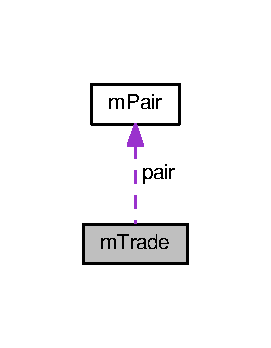
\includegraphics[width=130pt]{struct_k_1_1m_trade__coll__graph}
\end{center}
\end{figure}
\subsection*{Public Member Functions}
\begin{DoxyCompactItemize}
\item 
\hyperlink{struct_k_1_1m_trade_a645b1cd153838348bc43a21a1d5f70a4}{m\+Trade} ()
\item 
\hyperlink{struct_k_1_1m_trade_a34abd866cec68d1c3cc750375ecfd16a}{m\+Trade} (\hyperlink{km_8h_a392f9b7f384aa3539bbb890b059f5b8c}{m\+Price} p, \hyperlink{km_8h_ad4d00888c55a47a8a40ed8020d176086}{m\+Amount} \hyperlink{namespace_k_a211862d8b09ec46a051464b6859c1306a7694f4a66316e53c8cdd9d9954bd611d}{q}, \hyperlink{namespace_k_a0b7d0fa0ffc9f87da1d6499cbcee7e94}{m\+Side} s)
\item 
\hyperlink{struct_k_1_1m_trade_a48f7afc43dda9438c00f23f8578d3f69}{m\+Trade} (string i, \hyperlink{struct_k_1_1m_pair}{m\+Pair} P, \hyperlink{km_8h_a392f9b7f384aa3539bbb890b059f5b8c}{m\+Price} p, \hyperlink{km_8h_ad4d00888c55a47a8a40ed8020d176086}{m\+Amount} \hyperlink{namespace_k_a211862d8b09ec46a051464b6859c1306a7694f4a66316e53c8cdd9d9954bd611d}{q}, \hyperlink{namespace_k_a0b7d0fa0ffc9f87da1d6499cbcee7e94}{m\+Side} S, \hyperlink{km_8h_ad02a70cba4c52ba2013e5e32ceaeac1c}{m\+Clock} t, \hyperlink{km_8h_ad4d00888c55a47a8a40ed8020d176086}{m\+Amount} v, \hyperlink{km_8h_ad02a70cba4c52ba2013e5e32ceaeac1c}{m\+Clock} Kt, \hyperlink{km_8h_ad4d00888c55a47a8a40ed8020d176086}{m\+Amount} Kq, \hyperlink{km_8h_a392f9b7f384aa3539bbb890b059f5b8c}{m\+Price} Kp, \hyperlink{km_8h_ad4d00888c55a47a8a40ed8020d176086}{m\+Amount} Kv, \hyperlink{km_8h_ad4d00888c55a47a8a40ed8020d176086}{m\+Amount} Kd, \hyperlink{km_8h_ad4d00888c55a47a8a40ed8020d176086}{m\+Amount} f, bool l)
\end{DoxyCompactItemize}
\subsection*{Data Fields}
\begin{DoxyCompactItemize}
\item 
string \hyperlink{struct_k_1_1m_trade_a1a30d92defc429c8bd698cdacdb9749f}{trade\+Id}
\item 
\hyperlink{namespace_k_a0b7d0fa0ffc9f87da1d6499cbcee7e94}{m\+Side} \hyperlink{struct_k_1_1m_trade_afc5924267a11b19eb2f198a919a12351}{side}
\item 
\hyperlink{struct_k_1_1m_pair}{m\+Pair} \hyperlink{struct_k_1_1m_trade_a11dec7b102d6df830347649bfbf35399}{pair}
\item 
\hyperlink{km_8h_a392f9b7f384aa3539bbb890b059f5b8c}{m\+Price} \hyperlink{struct_k_1_1m_trade_a96d6f95b2441f538965c5d8c1aa32f4e}{price}
\item 
\hyperlink{km_8h_a392f9b7f384aa3539bbb890b059f5b8c}{m\+Price} \hyperlink{struct_k_1_1m_trade_affef8ad6bfa3b7c819981e40a4786444}{Kprice}
\item 
\hyperlink{km_8h_ad4d00888c55a47a8a40ed8020d176086}{m\+Amount} \hyperlink{struct_k_1_1m_trade_ab51872d3926e8302926e8ac851dbb158}{quantity}
\item 
\hyperlink{km_8h_ad4d00888c55a47a8a40ed8020d176086}{m\+Amount} \hyperlink{struct_k_1_1m_trade_a2c33cdf6b415658a577653196c59739a}{value}
\item 
\hyperlink{km_8h_ad4d00888c55a47a8a40ed8020d176086}{m\+Amount} \hyperlink{struct_k_1_1m_trade_ab4611562283514c0ca59af939c5c9abe}{Kqty}
\item 
\hyperlink{km_8h_ad4d00888c55a47a8a40ed8020d176086}{m\+Amount} \hyperlink{struct_k_1_1m_trade_af4444beba69e8718b065bb9d6f465ded}{Kvalue}
\item 
\hyperlink{km_8h_ad4d00888c55a47a8a40ed8020d176086}{m\+Amount} \hyperlink{struct_k_1_1m_trade_afc10958762dbc38c54aa501fcc84d42a}{Kdiff}
\item 
\hyperlink{km_8h_ad4d00888c55a47a8a40ed8020d176086}{m\+Amount} \hyperlink{struct_k_1_1m_trade_a5668f9fd404b2b486f72848972cc3add}{fee\+Charged}
\item 
\hyperlink{km_8h_ad02a70cba4c52ba2013e5e32ceaeac1c}{m\+Clock} \hyperlink{struct_k_1_1m_trade_a8c7be9fac36539b28a92dd5240ec377b}{time}
\item 
\hyperlink{km_8h_ad02a70cba4c52ba2013e5e32ceaeac1c}{m\+Clock} \hyperlink{struct_k_1_1m_trade_a55e39653e425359e6d8f7de1e6e792de}{Ktime}
\item 
bool \hyperlink{struct_k_1_1m_trade_a7bef80571660471d5752c5e1b71450ff}{loaded\+From\+DB}
\end{DoxyCompactItemize}


\subsection{Detailed Description}


Definition at line 409 of file km.\+h.



\subsection{Constructor \& Destructor Documentation}
\index{K\+::m\+Trade@{K\+::m\+Trade}!m\+Trade@{m\+Trade}}
\index{m\+Trade@{m\+Trade}!K\+::m\+Trade@{K\+::m\+Trade}}
\subsubsection[{\texorpdfstring{m\+Trade()}{mTrade()}}]{\setlength{\rightskip}{0pt plus 5cm}{\bf m\+Trade} (
\begin{DoxyParamCaption}
{}
\end{DoxyParamCaption}
)\hspace{0.3cm}{\ttfamily [inline]}}\hypertarget{struct_k_1_1m_trade_a645b1cd153838348bc43a21a1d5f70a4}{}\label{struct_k_1_1m_trade_a645b1cd153838348bc43a21a1d5f70a4}


Definition at line 424 of file km.\+h.

\index{K\+::m\+Trade@{K\+::m\+Trade}!m\+Trade@{m\+Trade}}
\index{m\+Trade@{m\+Trade}!K\+::m\+Trade@{K\+::m\+Trade}}
\subsubsection[{\texorpdfstring{m\+Trade(m\+Price p, m\+Amount q, m\+Side s)}{mTrade(mPrice p, mAmount q, mSide s)}}]{\setlength{\rightskip}{0pt plus 5cm}{\bf m\+Trade} (
\begin{DoxyParamCaption}
\item[{{\bf m\+Price}}]{p, }
\item[{{\bf m\+Amount}}]{q, }
\item[{{\bf m\+Side}}]{s}
\end{DoxyParamCaption}
)\hspace{0.3cm}{\ttfamily [inline]}}\hypertarget{struct_k_1_1m_trade_a34abd866cec68d1c3cc750375ecfd16a}{}\label{struct_k_1_1m_trade_a34abd866cec68d1c3cc750375ecfd16a}


Definition at line 427 of file km.\+h.

\index{K\+::m\+Trade@{K\+::m\+Trade}!m\+Trade@{m\+Trade}}
\index{m\+Trade@{m\+Trade}!K\+::m\+Trade@{K\+::m\+Trade}}
\subsubsection[{\texorpdfstring{m\+Trade(string i, m\+Pair P, m\+Price p, m\+Amount q, m\+Side S, m\+Clock t, m\+Amount v, m\+Clock Kt, m\+Amount Kq, m\+Price Kp, m\+Amount Kv, m\+Amount Kd, m\+Amount f, bool l)}{mTrade(string i, mPair P, mPrice p, mAmount q, mSide S, mClock t, mAmount v, mClock Kt, mAmount Kq, mPrice Kp, mAmount Kv, mAmount Kd, mAmount f, bool l)}}]{\setlength{\rightskip}{0pt plus 5cm}{\bf m\+Trade} (
\begin{DoxyParamCaption}
\item[{string}]{i, }
\item[{{\bf m\+Pair}}]{P, }
\item[{{\bf m\+Price}}]{p, }
\item[{{\bf m\+Amount}}]{q, }
\item[{{\bf m\+Side}}]{S, }
\item[{{\bf m\+Clock}}]{t, }
\item[{{\bf m\+Amount}}]{v, }
\item[{{\bf m\+Clock}}]{Kt, }
\item[{{\bf m\+Amount}}]{Kq, }
\item[{{\bf m\+Price}}]{Kp, }
\item[{{\bf m\+Amount}}]{Kv, }
\item[{{\bf m\+Amount}}]{Kd, }
\item[{{\bf m\+Amount}}]{f, }
\item[{bool}]{l}
\end{DoxyParamCaption}
)\hspace{0.3cm}{\ttfamily [inline]}}\hypertarget{struct_k_1_1m_trade_a48f7afc43dda9438c00f23f8578d3f69}{}\label{struct_k_1_1m_trade_a48f7afc43dda9438c00f23f8578d3f69}


Definition at line 430 of file km.\+h.



\subsection{Field Documentation}
\index{K\+::m\+Trade@{K\+::m\+Trade}!fee\+Charged@{fee\+Charged}}
\index{fee\+Charged@{fee\+Charged}!K\+::m\+Trade@{K\+::m\+Trade}}
\subsubsection[{\texorpdfstring{fee\+Charged}{feeCharged}}]{\setlength{\rightskip}{0pt plus 5cm}{\bf m\+Amount} fee\+Charged}\hypertarget{struct_k_1_1m_trade_a5668f9fd404b2b486f72848972cc3add}{}\label{struct_k_1_1m_trade_a5668f9fd404b2b486f72848972cc3add}


Definition at line 415 of file km.\+h.

\index{K\+::m\+Trade@{K\+::m\+Trade}!Kdiff@{Kdiff}}
\index{Kdiff@{Kdiff}!K\+::m\+Trade@{K\+::m\+Trade}}
\subsubsection[{\texorpdfstring{Kdiff}{Kdiff}}]{\setlength{\rightskip}{0pt plus 5cm}{\bf m\+Amount} Kdiff}\hypertarget{struct_k_1_1m_trade_afc10958762dbc38c54aa501fcc84d42a}{}\label{struct_k_1_1m_trade_afc10958762dbc38c54aa501fcc84d42a}


Definition at line 415 of file km.\+h.

\index{K\+::m\+Trade@{K\+::m\+Trade}!Kprice@{Kprice}}
\index{Kprice@{Kprice}!K\+::m\+Trade@{K\+::m\+Trade}}
\subsubsection[{\texorpdfstring{Kprice}{Kprice}}]{\setlength{\rightskip}{0pt plus 5cm}{\bf m\+Price} Kprice}\hypertarget{struct_k_1_1m_trade_affef8ad6bfa3b7c819981e40a4786444}{}\label{struct_k_1_1m_trade_affef8ad6bfa3b7c819981e40a4786444}


Definition at line 413 of file km.\+h.

\index{K\+::m\+Trade@{K\+::m\+Trade}!Kqty@{Kqty}}
\index{Kqty@{Kqty}!K\+::m\+Trade@{K\+::m\+Trade}}
\subsubsection[{\texorpdfstring{Kqty}{Kqty}}]{\setlength{\rightskip}{0pt plus 5cm}{\bf m\+Amount} Kqty}\hypertarget{struct_k_1_1m_trade_ab4611562283514c0ca59af939c5c9abe}{}\label{struct_k_1_1m_trade_ab4611562283514c0ca59af939c5c9abe}


Definition at line 415 of file km.\+h.

\index{K\+::m\+Trade@{K\+::m\+Trade}!Ktime@{Ktime}}
\index{Ktime@{Ktime}!K\+::m\+Trade@{K\+::m\+Trade}}
\subsubsection[{\texorpdfstring{Ktime}{Ktime}}]{\setlength{\rightskip}{0pt plus 5cm}{\bf m\+Clock} Ktime}\hypertarget{struct_k_1_1m_trade_a55e39653e425359e6d8f7de1e6e792de}{}\label{struct_k_1_1m_trade_a55e39653e425359e6d8f7de1e6e792de}


Definition at line 421 of file km.\+h.

\index{K\+::m\+Trade@{K\+::m\+Trade}!Kvalue@{Kvalue}}
\index{Kvalue@{Kvalue}!K\+::m\+Trade@{K\+::m\+Trade}}
\subsubsection[{\texorpdfstring{Kvalue}{Kvalue}}]{\setlength{\rightskip}{0pt plus 5cm}{\bf m\+Amount} Kvalue}\hypertarget{struct_k_1_1m_trade_af4444beba69e8718b065bb9d6f465ded}{}\label{struct_k_1_1m_trade_af4444beba69e8718b065bb9d6f465ded}


Definition at line 415 of file km.\+h.

\index{K\+::m\+Trade@{K\+::m\+Trade}!loaded\+From\+DB@{loaded\+From\+DB}}
\index{loaded\+From\+DB@{loaded\+From\+DB}!K\+::m\+Trade@{K\+::m\+Trade}}
\subsubsection[{\texorpdfstring{loaded\+From\+DB}{loadedFromDB}}]{\setlength{\rightskip}{0pt plus 5cm}bool loaded\+From\+DB}\hypertarget{struct_k_1_1m_trade_a7bef80571660471d5752c5e1b71450ff}{}\label{struct_k_1_1m_trade_a7bef80571660471d5752c5e1b71450ff}


Definition at line 423 of file km.\+h.

\index{K\+::m\+Trade@{K\+::m\+Trade}!pair@{pair}}
\index{pair@{pair}!K\+::m\+Trade@{K\+::m\+Trade}}
\subsubsection[{\texorpdfstring{pair}{pair}}]{\setlength{\rightskip}{0pt plus 5cm}{\bf m\+Pair} pair}\hypertarget{struct_k_1_1m_trade_a11dec7b102d6df830347649bfbf35399}{}\label{struct_k_1_1m_trade_a11dec7b102d6df830347649bfbf35399}


Definition at line 412 of file km.\+h.

\index{K\+::m\+Trade@{K\+::m\+Trade}!price@{price}}
\index{price@{price}!K\+::m\+Trade@{K\+::m\+Trade}}
\subsubsection[{\texorpdfstring{price}{price}}]{\setlength{\rightskip}{0pt plus 5cm}{\bf m\+Price} price}\hypertarget{struct_k_1_1m_trade_a96d6f95b2441f538965c5d8c1aa32f4e}{}\label{struct_k_1_1m_trade_a96d6f95b2441f538965c5d8c1aa32f4e}


Definition at line 413 of file km.\+h.

\index{K\+::m\+Trade@{K\+::m\+Trade}!quantity@{quantity}}
\index{quantity@{quantity}!K\+::m\+Trade@{K\+::m\+Trade}}
\subsubsection[{\texorpdfstring{quantity}{quantity}}]{\setlength{\rightskip}{0pt plus 5cm}{\bf m\+Amount} quantity}\hypertarget{struct_k_1_1m_trade_ab51872d3926e8302926e8ac851dbb158}{}\label{struct_k_1_1m_trade_ab51872d3926e8302926e8ac851dbb158}


Definition at line 415 of file km.\+h.

\index{K\+::m\+Trade@{K\+::m\+Trade}!side@{side}}
\index{side@{side}!K\+::m\+Trade@{K\+::m\+Trade}}
\subsubsection[{\texorpdfstring{side}{side}}]{\setlength{\rightskip}{0pt plus 5cm}{\bf m\+Side} side}\hypertarget{struct_k_1_1m_trade_afc5924267a11b19eb2f198a919a12351}{}\label{struct_k_1_1m_trade_afc5924267a11b19eb2f198a919a12351}


Definition at line 411 of file km.\+h.

\index{K\+::m\+Trade@{K\+::m\+Trade}!time@{time}}
\index{time@{time}!K\+::m\+Trade@{K\+::m\+Trade}}
\subsubsection[{\texorpdfstring{time}{time}}]{\setlength{\rightskip}{0pt plus 5cm}{\bf m\+Clock} time}\hypertarget{struct_k_1_1m_trade_a8c7be9fac36539b28a92dd5240ec377b}{}\label{struct_k_1_1m_trade_a8c7be9fac36539b28a92dd5240ec377b}


Definition at line 421 of file km.\+h.

\index{K\+::m\+Trade@{K\+::m\+Trade}!trade\+Id@{trade\+Id}}
\index{trade\+Id@{trade\+Id}!K\+::m\+Trade@{K\+::m\+Trade}}
\subsubsection[{\texorpdfstring{trade\+Id}{tradeId}}]{\setlength{\rightskip}{0pt plus 5cm}string trade\+Id}\hypertarget{struct_k_1_1m_trade_a1a30d92defc429c8bd698cdacdb9749f}{}\label{struct_k_1_1m_trade_a1a30d92defc429c8bd698cdacdb9749f}


Definition at line 410 of file km.\+h.

\index{K\+::m\+Trade@{K\+::m\+Trade}!value@{value}}
\index{value@{value}!K\+::m\+Trade@{K\+::m\+Trade}}
\subsubsection[{\texorpdfstring{value}{value}}]{\setlength{\rightskip}{0pt plus 5cm}{\bf m\+Amount} value}\hypertarget{struct_k_1_1m_trade_a2c33cdf6b415658a577653196c59739a}{}\label{struct_k_1_1m_trade_a2c33cdf6b415658a577653196c59739a}


Definition at line 415 of file km.\+h.



The documentation for this struct was generated from the following file\+:\begin{DoxyCompactItemize}
\item 
\hyperlink{km_8h}{km.\+h}\end{DoxyCompactItemize}

\hypertarget{struct_k_1_1m_wallet}{}\section{m\+Wallet Struct Reference}
\label{struct_k_1_1m_wallet}\index{m\+Wallet@{m\+Wallet}}


{\ttfamily \#include $<$km.\+h$>$}

\subsection*{Public Member Functions}
\begin{DoxyCompactItemize}
\item 
\hyperlink{struct_k_1_1m_wallet_a97ad90c2a76dabc6504f1317490bb2b9}{m\+Wallet} ()
\item 
\hyperlink{struct_k_1_1m_wallet_a1e8eab2393719ed37777cc3372044d80}{m\+Wallet} (\hyperlink{km_8h_ad4d00888c55a47a8a40ed8020d176086}{m\+Amount} a, \hyperlink{km_8h_ad4d00888c55a47a8a40ed8020d176086}{m\+Amount} h, \hyperlink{km_8h_a0299927fb26276a1e0f4c2b4dedb698e}{m\+Coin\+Id} c)
\item 
void \hyperlink{struct_k_1_1m_wallet_a853c23fdf7cba1e1005c5b59769642ba}{reset} (\hyperlink{km_8h_ad4d00888c55a47a8a40ed8020d176086}{m\+Amount} a, \hyperlink{km_8h_ad4d00888c55a47a8a40ed8020d176086}{m\+Amount} h)
\item 
bool \hyperlink{struct_k_1_1m_wallet_a3f37b042a1e7cd4bd38fc564de81f0da}{empty} ()
\end{DoxyCompactItemize}
\subsection*{Data Fields}
\begin{DoxyCompactItemize}
\item 
\hyperlink{km_8h_ad4d00888c55a47a8a40ed8020d176086}{m\+Amount} \hyperlink{struct_k_1_1m_wallet_a45ae71aeec90c6a39f4ba8187ae01345}{amount}
\item 
\hyperlink{km_8h_ad4d00888c55a47a8a40ed8020d176086}{m\+Amount} \hyperlink{struct_k_1_1m_wallet_a9b5165456071402b08d8b71ce5c2e9d0}{held}
\item 
\hyperlink{km_8h_a0299927fb26276a1e0f4c2b4dedb698e}{m\+Coin\+Id} \hyperlink{struct_k_1_1m_wallet_a216d44ca9942257997747da567464473}{currency}
\end{DoxyCompactItemize}


\subsection{Detailed Description}


Definition at line 271 of file km.\+h.



\subsection{Constructor \& Destructor Documentation}
\index{K\+::m\+Wallet@{K\+::m\+Wallet}!m\+Wallet@{m\+Wallet}}
\index{m\+Wallet@{m\+Wallet}!K\+::m\+Wallet@{K\+::m\+Wallet}}
\subsubsection[{\texorpdfstring{m\+Wallet()}{mWallet()}}]{\setlength{\rightskip}{0pt plus 5cm}{\bf m\+Wallet} (
\begin{DoxyParamCaption}
{}
\end{DoxyParamCaption}
)\hspace{0.3cm}{\ttfamily [inline]}}\hypertarget{struct_k_1_1m_wallet_a97ad90c2a76dabc6504f1317490bb2b9}{}\label{struct_k_1_1m_wallet_a97ad90c2a76dabc6504f1317490bb2b9}


Definition at line 275 of file km.\+h.

\index{K\+::m\+Wallet@{K\+::m\+Wallet}!m\+Wallet@{m\+Wallet}}
\index{m\+Wallet@{m\+Wallet}!K\+::m\+Wallet@{K\+::m\+Wallet}}
\subsubsection[{\texorpdfstring{m\+Wallet(m\+Amount a, m\+Amount h, m\+Coin\+Id c)}{mWallet(mAmount a, mAmount h, mCoinId c)}}]{\setlength{\rightskip}{0pt plus 5cm}{\bf m\+Wallet} (
\begin{DoxyParamCaption}
\item[{{\bf m\+Amount}}]{a, }
\item[{{\bf m\+Amount}}]{h, }
\item[{{\bf m\+Coin\+Id}}]{c}
\end{DoxyParamCaption}
)\hspace{0.3cm}{\ttfamily [inline]}}\hypertarget{struct_k_1_1m_wallet_a1e8eab2393719ed37777cc3372044d80}{}\label{struct_k_1_1m_wallet_a1e8eab2393719ed37777cc3372044d80}


Definition at line 278 of file km.\+h.



\subsection{Member Function Documentation}
\index{K\+::m\+Wallet@{K\+::m\+Wallet}!empty@{empty}}
\index{empty@{empty}!K\+::m\+Wallet@{K\+::m\+Wallet}}
\subsubsection[{\texorpdfstring{empty()}{empty()}}]{\setlength{\rightskip}{0pt plus 5cm}bool empty (
\begin{DoxyParamCaption}
{}
\end{DoxyParamCaption}
)\hspace{0.3cm}{\ttfamily [inline]}}\hypertarget{struct_k_1_1m_wallet_a3f37b042a1e7cd4bd38fc564de81f0da}{}\label{struct_k_1_1m_wallet_a3f37b042a1e7cd4bd38fc564de81f0da}


Definition at line 286 of file km.\+h.

\index{K\+::m\+Wallet@{K\+::m\+Wallet}!reset@{reset}}
\index{reset@{reset}!K\+::m\+Wallet@{K\+::m\+Wallet}}
\subsubsection[{\texorpdfstring{reset(m\+Amount a, m\+Amount h)}{reset(mAmount a, mAmount h)}}]{\setlength{\rightskip}{0pt plus 5cm}void reset (
\begin{DoxyParamCaption}
\item[{{\bf m\+Amount}}]{a, }
\item[{{\bf m\+Amount}}]{h}
\end{DoxyParamCaption}
)\hspace{0.3cm}{\ttfamily [inline]}}\hypertarget{struct_k_1_1m_wallet_a853c23fdf7cba1e1005c5b59769642ba}{}\label{struct_k_1_1m_wallet_a853c23fdf7cba1e1005c5b59769642ba}


Definition at line 281 of file km.\+h.



\subsection{Field Documentation}
\index{K\+::m\+Wallet@{K\+::m\+Wallet}!amount@{amount}}
\index{amount@{amount}!K\+::m\+Wallet@{K\+::m\+Wallet}}
\subsubsection[{\texorpdfstring{amount}{amount}}]{\setlength{\rightskip}{0pt plus 5cm}{\bf m\+Amount} amount}\hypertarget{struct_k_1_1m_wallet_a45ae71aeec90c6a39f4ba8187ae01345}{}\label{struct_k_1_1m_wallet_a45ae71aeec90c6a39f4ba8187ae01345}


Definition at line 272 of file km.\+h.

\index{K\+::m\+Wallet@{K\+::m\+Wallet}!currency@{currency}}
\index{currency@{currency}!K\+::m\+Wallet@{K\+::m\+Wallet}}
\subsubsection[{\texorpdfstring{currency}{currency}}]{\setlength{\rightskip}{0pt plus 5cm}{\bf m\+Coin\+Id} currency}\hypertarget{struct_k_1_1m_wallet_a216d44ca9942257997747da567464473}{}\label{struct_k_1_1m_wallet_a216d44ca9942257997747da567464473}


Definition at line 274 of file km.\+h.

\index{K\+::m\+Wallet@{K\+::m\+Wallet}!held@{held}}
\index{held@{held}!K\+::m\+Wallet@{K\+::m\+Wallet}}
\subsubsection[{\texorpdfstring{held}{held}}]{\setlength{\rightskip}{0pt plus 5cm}{\bf m\+Amount} held}\hypertarget{struct_k_1_1m_wallet_a9b5165456071402b08d8b71ce5c2e9d0}{}\label{struct_k_1_1m_wallet_a9b5165456071402b08d8b71ce5c2e9d0}


Definition at line 272 of file km.\+h.



The documentation for this struct was generated from the following file\+:\begin{DoxyCompactItemize}
\item 
\hyperlink{km_8h}{km.\+h}\end{DoxyCompactItemize}

\hypertarget{struct_k_1_1m_wallets}{}\section{m\+Wallets Struct Reference}
\label{struct_k_1_1m_wallets}\index{m\+Wallets@{m\+Wallets}}


{\ttfamily \#include $<$km.\+h$>$}



Collaboration diagram for m\+Wallets\+:
\nopagebreak
\begin{figure}[H]
\begin{center}
\leavevmode
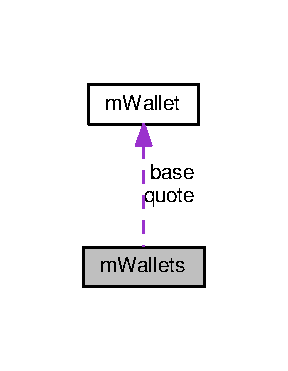
\includegraphics[width=138pt]{struct_k_1_1m_wallets__coll__graph}
\end{center}
\end{figure}
\subsection*{Public Member Functions}
\begin{DoxyCompactItemize}
\item 
\hyperlink{struct_k_1_1m_wallets_abcd72a711936c5391f4182544c9f9c84}{m\+Wallets} ()
\item 
\hyperlink{struct_k_1_1m_wallets_a97f25778ffc81e82ea69d0d9ecaa45d3}{m\+Wallets} (\hyperlink{struct_k_1_1m_wallet}{m\+Wallet} b, \hyperlink{struct_k_1_1m_wallet}{m\+Wallet} \hyperlink{namespace_k_a211862d8b09ec46a051464b6859c1306a7694f4a66316e53c8cdd9d9954bd611d}{q})
\item 
bool \hyperlink{struct_k_1_1m_wallets_a3f37b042a1e7cd4bd38fc564de81f0da}{empty} ()
\end{DoxyCompactItemize}
\subsection*{Data Fields}
\begin{DoxyCompactItemize}
\item 
\hyperlink{struct_k_1_1m_wallet}{m\+Wallet} \hyperlink{struct_k_1_1m_wallets_aa296cf3f15f714fd4d6d28a58fa2a86e}{base}
\item 
\hyperlink{struct_k_1_1m_wallet}{m\+Wallet} \hyperlink{struct_k_1_1m_wallets_a8845af0197ce15438cc6ad3e860259a8}{quote}
\end{DoxyCompactItemize}


\subsection{Detailed Description}


Definition at line 297 of file km.\+h.



\subsection{Constructor \& Destructor Documentation}
\index{K\+::m\+Wallets@{K\+::m\+Wallets}!m\+Wallets@{m\+Wallets}}
\index{m\+Wallets@{m\+Wallets}!K\+::m\+Wallets@{K\+::m\+Wallets}}
\subsubsection[{\texorpdfstring{m\+Wallets()}{mWallets()}}]{\setlength{\rightskip}{0pt plus 5cm}{\bf m\+Wallets} (
\begin{DoxyParamCaption}
{}
\end{DoxyParamCaption}
)\hspace{0.3cm}{\ttfamily [inline]}}\hypertarget{struct_k_1_1m_wallets_abcd72a711936c5391f4182544c9f9c84}{}\label{struct_k_1_1m_wallets_abcd72a711936c5391f4182544c9f9c84}


Definition at line 300 of file km.\+h.

\index{K\+::m\+Wallets@{K\+::m\+Wallets}!m\+Wallets@{m\+Wallets}}
\index{m\+Wallets@{m\+Wallets}!K\+::m\+Wallets@{K\+::m\+Wallets}}
\subsubsection[{\texorpdfstring{m\+Wallets(m\+Wallet b, m\+Wallet q)}{mWallets(mWallet b, mWallet q)}}]{\setlength{\rightskip}{0pt plus 5cm}{\bf m\+Wallets} (
\begin{DoxyParamCaption}
\item[{{\bf m\+Wallet}}]{b, }
\item[{{\bf m\+Wallet}}]{q}
\end{DoxyParamCaption}
)\hspace{0.3cm}{\ttfamily [inline]}}\hypertarget{struct_k_1_1m_wallets_a97f25778ffc81e82ea69d0d9ecaa45d3}{}\label{struct_k_1_1m_wallets_a97f25778ffc81e82ea69d0d9ecaa45d3}


Definition at line 303 of file km.\+h.



\subsection{Member Function Documentation}
\index{K\+::m\+Wallets@{K\+::m\+Wallets}!empty@{empty}}
\index{empty@{empty}!K\+::m\+Wallets@{K\+::m\+Wallets}}
\subsubsection[{\texorpdfstring{empty()}{empty()}}]{\setlength{\rightskip}{0pt plus 5cm}bool empty (
\begin{DoxyParamCaption}
{}
\end{DoxyParamCaption}
)\hspace{0.3cm}{\ttfamily [inline]}}\hypertarget{struct_k_1_1m_wallets_a3f37b042a1e7cd4bd38fc564de81f0da}{}\label{struct_k_1_1m_wallets_a3f37b042a1e7cd4bd38fc564de81f0da}


Definition at line 306 of file km.\+h.



\subsection{Field Documentation}
\index{K\+::m\+Wallets@{K\+::m\+Wallets}!base@{base}}
\index{base@{base}!K\+::m\+Wallets@{K\+::m\+Wallets}}
\subsubsection[{\texorpdfstring{base}{base}}]{\setlength{\rightskip}{0pt plus 5cm}{\bf m\+Wallet} base}\hypertarget{struct_k_1_1m_wallets_aa296cf3f15f714fd4d6d28a58fa2a86e}{}\label{struct_k_1_1m_wallets_aa296cf3f15f714fd4d6d28a58fa2a86e}


Definition at line 298 of file km.\+h.

\index{K\+::m\+Wallets@{K\+::m\+Wallets}!quote@{quote}}
\index{quote@{quote}!K\+::m\+Wallets@{K\+::m\+Wallets}}
\subsubsection[{\texorpdfstring{quote}{quote}}]{\setlength{\rightskip}{0pt plus 5cm}{\bf m\+Wallet} quote}\hypertarget{struct_k_1_1m_wallets_a8845af0197ce15438cc6ad3e860259a8}{}\label{struct_k_1_1m_wallets_a8845af0197ce15438cc6ad3e860259a8}


Definition at line 298 of file km.\+h.



The documentation for this struct was generated from the following file\+:\begin{DoxyCompactItemize}
\item 
\hyperlink{km_8h}{km.\+h}\end{DoxyCompactItemize}

\hypertarget{class_k_1_1_o_g}{}\section{OG Class Reference}
\label{class_k_1_1_o_g}\index{OG@{OG}}


{\ttfamily \#include $<$og.\+h$>$}



Inheritance diagram for OG\+:
\nopagebreak
\begin{figure}[H]
\begin{center}
\leavevmode
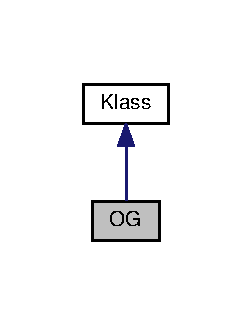
\includegraphics[width=121pt]{class_k_1_1_o_g__inherit__graph}
\end{center}
\end{figure}


Collaboration diagram for OG\+:
\nopagebreak
\begin{figure}[H]
\begin{center}
\leavevmode
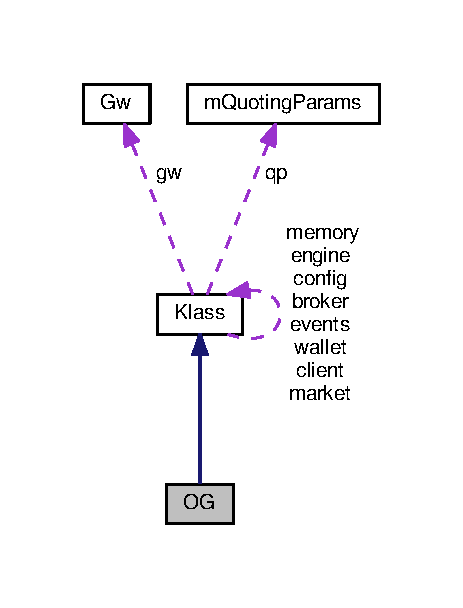
\includegraphics[width=222pt]{class_k_1_1_o_g__coll__graph}
\end{center}
\end{figure}
\subsection*{Public Member Functions}
\begin{DoxyCompactItemize}
\item 
void \hyperlink{class_k_1_1_o_g_a1abe610a042782fc064f909adf519013}{send\+Order} (vector$<$ \hyperlink{km_8h_a23233b27e494114073abc4d494b05626}{m\+Rand\+Id} $>$ to\+Cancel, \hyperlink{namespace_k_a0b7d0fa0ffc9f87da1d6499cbcee7e94}{m\+Side} side, \hyperlink{km_8h_a392f9b7f384aa3539bbb890b059f5b8c}{m\+Price} price, \hyperlink{km_8h_ad4d00888c55a47a8a40ed8020d176086}{m\+Amount} qty, \hyperlink{namespace_k_a131435180aff10fab1bf3da09af62b0d}{m\+Order\+Type} type, \hyperlink{namespace_k_a290fccb3fc7d447fdbb93a61f6dfba44}{m\+Time\+In\+Force} tif, bool is\+Pong, bool post\+Only)
\item 
void \hyperlink{class_k_1_1_o_g_a9b8d071fe7202c65f78901a02a1e04d6}{cancel\+Order} (\hyperlink{km_8h_a23233b27e494114073abc4d494b05626}{m\+Rand\+Id} order\+Id)
\item 
void \hyperlink{class_k_1_1_o_g_ab503bb642cb730d5be83e54c16a6e7e7}{clean\+Order} (\hyperlink{km_8h_a23233b27e494114073abc4d494b05626}{m\+Rand\+Id} \&order\+Id)
\end{DoxyCompactItemize}
\subsection*{Data Fields}
\begin{DoxyCompactItemize}
\item 
map$<$ \hyperlink{km_8h_a23233b27e494114073abc4d494b05626}{m\+Rand\+Id}, \hyperlink{struct_k_1_1m_order}{m\+Order} $>$ \hyperlink{class_k_1_1_o_g_a3edc39f2b61ed046bfac9414042e54c4}{orders}
\item 
vector$<$ \hyperlink{struct_k_1_1m_trade}{m\+Trade} $>$ \hyperlink{class_k_1_1_o_g_a4b64cd03cacdbed4ca7d0b7151546441}{trades\+History}
\item 
function$<$ void(\hyperlink{namespace_k_a0b7d0fa0ffc9f87da1d6499cbcee7e94}{m\+Side}, bool)$>$ $\ast$ \hyperlink{class_k_1_1_o_g_a61416b97cde02a422eb91f3d29ef346f}{calc\+Wallet\+After\+Order} = nullptr
\item 
function$<$ void(\hyperlink{struct_k_1_1m_trade}{m\+Trade} $\ast$)$>$ $\ast$ \hyperlink{class_k_1_1_o_g_a58a0b5975f3806226227956a06f57432}{calc\+Safety\+After\+Trade} = nullptr
\end{DoxyCompactItemize}
\subsection*{Protected Member Functions}
\begin{DoxyCompactItemize}
\item 
void \hyperlink{class_k_1_1_o_g_a78f61ac2dd03bcba8e09ca20cd7d68e3}{load} ()
\item 
void \hyperlink{class_k_1_1_o_g_aa9a0f090ee360e2a9f967200d30f4a22}{wait\+Data} ()
\item 
void \hyperlink{class_k_1_1_o_g_aa3f7b56799f5915cfbc902f6426c2bb2}{wait\+User} ()
\item 
void \hyperlink{class_k_1_1_o_g_a13a43e6d814de94978c515cb084873b1}{run} ()
\end{DoxyCompactItemize}
\subsection*{Additional Inherited Members}


\subsection{Detailed Description}


Definition at line 5 of file og.\+h.



\subsection{Member Function Documentation}
\index{K\+::\+OG@{K\+::\+OG}!cancel\+Order@{cancel\+Order}}
\index{cancel\+Order@{cancel\+Order}!K\+::\+OG@{K\+::\+OG}}
\subsubsection[{\texorpdfstring{cancel\+Order(m\+Rand\+Id order\+Id)}{cancelOrder(mRandId orderId)}}]{\setlength{\rightskip}{0pt plus 5cm}void cancel\+Order (
\begin{DoxyParamCaption}
\item[{{\bf m\+Rand\+Id}}]{order\+Id}
\end{DoxyParamCaption}
)\hspace{0.3cm}{\ttfamily [inline]}}\hypertarget{class_k_1_1_o_g_a9b8d071fe7202c65f78901a02a1e04d6}{}\label{class_k_1_1_o_g_a9b8d071fe7202c65f78901a02a1e04d6}


Definition at line 57 of file og.\+h.

\index{K\+::\+OG@{K\+::\+OG}!clean\+Order@{clean\+Order}}
\index{clean\+Order@{clean\+Order}!K\+::\+OG@{K\+::\+OG}}
\subsubsection[{\texorpdfstring{clean\+Order(m\+Rand\+Id \&order\+Id)}{cleanOrder(mRandId &orderId)}}]{\setlength{\rightskip}{0pt plus 5cm}void clean\+Order (
\begin{DoxyParamCaption}
\item[{{\bf m\+Rand\+Id} \&}]{order\+Id}
\end{DoxyParamCaption}
)\hspace{0.3cm}{\ttfamily [inline]}}\hypertarget{class_k_1_1_o_g_ab503bb642cb730d5be83e54c16a6e7e7}{}\label{class_k_1_1_o_g_ab503bb642cb730d5be83e54c16a6e7e7}


Definition at line 64 of file og.\+h.

\index{K\+::\+OG@{K\+::\+OG}!load@{load}}
\index{load@{load}!K\+::\+OG@{K\+::\+OG}}
\subsubsection[{\texorpdfstring{load()}{load()}}]{\setlength{\rightskip}{0pt plus 5cm}void load (
\begin{DoxyParamCaption}
{}
\end{DoxyParamCaption}
)\hspace{0.3cm}{\ttfamily [inline]}, {\ttfamily [protected]}, {\ttfamily [virtual]}}\hypertarget{class_k_1_1_o_g_a78f61ac2dd03bcba8e09ca20cd7d68e3}{}\label{class_k_1_1_o_g_a78f61ac2dd03bcba8e09ca20cd7d68e3}


Reimplemented from \hyperlink{class_k_1_1_klass_a5588964fff1d1025245d134e159b60ee}{Klass}.



Definition at line 12 of file og.\+h.

\index{K\+::\+OG@{K\+::\+OG}!run@{run}}
\index{run@{run}!K\+::\+OG@{K\+::\+OG}}
\subsubsection[{\texorpdfstring{run()}{run()}}]{\setlength{\rightskip}{0pt plus 5cm}void run (
\begin{DoxyParamCaption}
{}
\end{DoxyParamCaption}
)\hspace{0.3cm}{\ttfamily [inline]}, {\ttfamily [protected]}, {\ttfamily [virtual]}}\hypertarget{class_k_1_1_o_g_a13a43e6d814de94978c515cb084873b1}{}\label{class_k_1_1_o_g_a13a43e6d814de94978c515cb084873b1}


Reimplemented from \hyperlink{class_k_1_1_klass_a72fcb26a14f6beb1c3fbace9ab3e7dbb}{Klass}.



Definition at line 33 of file og.\+h.

\index{K\+::\+OG@{K\+::\+OG}!send\+Order@{send\+Order}}
\index{send\+Order@{send\+Order}!K\+::\+OG@{K\+::\+OG}}
\subsubsection[{\texorpdfstring{send\+Order(vector$<$ m\+Rand\+Id $>$ to\+Cancel, m\+Side side, m\+Price price, m\+Amount qty, m\+Order\+Type type, m\+Time\+In\+Force tif, bool is\+Pong, bool post\+Only)}{sendOrder(vector< mRandId > toCancel, mSide side, mPrice price, mAmount qty, mOrderType type, mTimeInForce tif, bool isPong, bool postOnly)}}]{\setlength{\rightskip}{0pt plus 5cm}void send\+Order (
\begin{DoxyParamCaption}
\item[{vector$<$ {\bf m\+Rand\+Id} $>$}]{to\+Cancel, }
\item[{{\bf m\+Side}}]{side, }
\item[{{\bf m\+Price}}]{price, }
\item[{{\bf m\+Amount}}]{qty, }
\item[{{\bf m\+Order\+Type}}]{type, }
\item[{{\bf m\+Time\+In\+Force}}]{tif, }
\item[{bool}]{is\+Pong, }
\item[{bool}]{post\+Only}
\end{DoxyParamCaption}
)\hspace{0.3cm}{\ttfamily [inline]}}\hypertarget{class_k_1_1_o_g_a1abe610a042782fc064f909adf519013}{}\label{class_k_1_1_o_g_a1abe610a042782fc064f909adf519013}


Definition at line 38 of file og.\+h.

\index{K\+::\+OG@{K\+::\+OG}!wait\+Data@{wait\+Data}}
\index{wait\+Data@{wait\+Data}!K\+::\+OG@{K\+::\+OG}}
\subsubsection[{\texorpdfstring{wait\+Data()}{waitData()}}]{\setlength{\rightskip}{0pt plus 5cm}void wait\+Data (
\begin{DoxyParamCaption}
{}
\end{DoxyParamCaption}
)\hspace{0.3cm}{\ttfamily [inline]}, {\ttfamily [protected]}, {\ttfamily [virtual]}}\hypertarget{class_k_1_1_o_g_aa9a0f090ee360e2a9f967200d30f4a22}{}\label{class_k_1_1_o_g_aa9a0f090ee360e2a9f967200d30f4a22}


Reimplemented from \hyperlink{class_k_1_1_klass_a62a6bf36d7c8bec9dcf7af20c9d21d74}{Klass}.



Definition at line 17 of file og.\+h.

\index{K\+::\+OG@{K\+::\+OG}!wait\+User@{wait\+User}}
\index{wait\+User@{wait\+User}!K\+::\+OG@{K\+::\+OG}}
\subsubsection[{\texorpdfstring{wait\+User()}{waitUser()}}]{\setlength{\rightskip}{0pt plus 5cm}void wait\+User (
\begin{DoxyParamCaption}
{}
\end{DoxyParamCaption}
)\hspace{0.3cm}{\ttfamily [inline]}, {\ttfamily [protected]}, {\ttfamily [virtual]}}\hypertarget{class_k_1_1_o_g_aa3f7b56799f5915cfbc902f6426c2bb2}{}\label{class_k_1_1_o_g_aa3f7b56799f5915cfbc902f6426c2bb2}


Reimplemented from \hyperlink{class_k_1_1_klass_af4f5201bed25a292d8a7f40470d83923}{Klass}.



Definition at line 23 of file og.\+h.



\subsection{Field Documentation}
\index{K\+::\+OG@{K\+::\+OG}!calc\+Safety\+After\+Trade@{calc\+Safety\+After\+Trade}}
\index{calc\+Safety\+After\+Trade@{calc\+Safety\+After\+Trade}!K\+::\+OG@{K\+::\+OG}}
\subsubsection[{\texorpdfstring{calc\+Safety\+After\+Trade}{calcSafetyAfterTrade}}]{\setlength{\rightskip}{0pt plus 5cm}function$<$void({\bf m\+Trade}$\ast$)$>$$\ast$ calc\+Safety\+After\+Trade = nullptr}\hypertarget{class_k_1_1_o_g_a58a0b5975f3806226227956a06f57432}{}\label{class_k_1_1_o_g_a58a0b5975f3806226227956a06f57432}


Definition at line 10 of file og.\+h.

\index{K\+::\+OG@{K\+::\+OG}!calc\+Wallet\+After\+Order@{calc\+Wallet\+After\+Order}}
\index{calc\+Wallet\+After\+Order@{calc\+Wallet\+After\+Order}!K\+::\+OG@{K\+::\+OG}}
\subsubsection[{\texorpdfstring{calc\+Wallet\+After\+Order}{calcWalletAfterOrder}}]{\setlength{\rightskip}{0pt plus 5cm}function$<$void({\bf m\+Side}, bool)$>$$\ast$ calc\+Wallet\+After\+Order = nullptr}\hypertarget{class_k_1_1_o_g_a61416b97cde02a422eb91f3d29ef346f}{}\label{class_k_1_1_o_g_a61416b97cde02a422eb91f3d29ef346f}


Definition at line 9 of file og.\+h.

\index{K\+::\+OG@{K\+::\+OG}!orders@{orders}}
\index{orders@{orders}!K\+::\+OG@{K\+::\+OG}}
\subsubsection[{\texorpdfstring{orders}{orders}}]{\setlength{\rightskip}{0pt plus 5cm}map$<${\bf m\+Rand\+Id}, {\bf m\+Order}$>$ orders}\hypertarget{class_k_1_1_o_g_a3edc39f2b61ed046bfac9414042e54c4}{}\label{class_k_1_1_o_g_a3edc39f2b61ed046bfac9414042e54c4}


Definition at line 7 of file og.\+h.

\index{K\+::\+OG@{K\+::\+OG}!trades\+History@{trades\+History}}
\index{trades\+History@{trades\+History}!K\+::\+OG@{K\+::\+OG}}
\subsubsection[{\texorpdfstring{trades\+History}{tradesHistory}}]{\setlength{\rightskip}{0pt plus 5cm}vector$<${\bf m\+Trade}$>$ trades\+History}\hypertarget{class_k_1_1_o_g_a4b64cd03cacdbed4ca7d0b7151546441}{}\label{class_k_1_1_o_g_a4b64cd03cacdbed4ca7d0b7151546441}


Definition at line 8 of file og.\+h.



The documentation for this class was generated from the following file\+:\begin{DoxyCompactItemize}
\item 
\hyperlink{og_8h}{og.\+h}\end{DoxyCompactItemize}

\hypertarget{class_k_1_1_p_g}{}\section{PG Class Reference}
\label{class_k_1_1_p_g}\index{PG@{PG}}


{\ttfamily \#include $<$pg.\+h$>$}



Inheritance diagram for PG\+:
\nopagebreak
\begin{figure}[H]
\begin{center}
\leavevmode
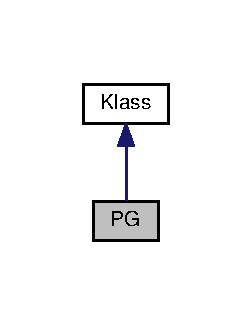
\includegraphics[width=121pt]{class_k_1_1_p_g__inherit__graph}
\end{center}
\end{figure}


Collaboration diagram for PG\+:
\nopagebreak
\begin{figure}[H]
\begin{center}
\leavevmode
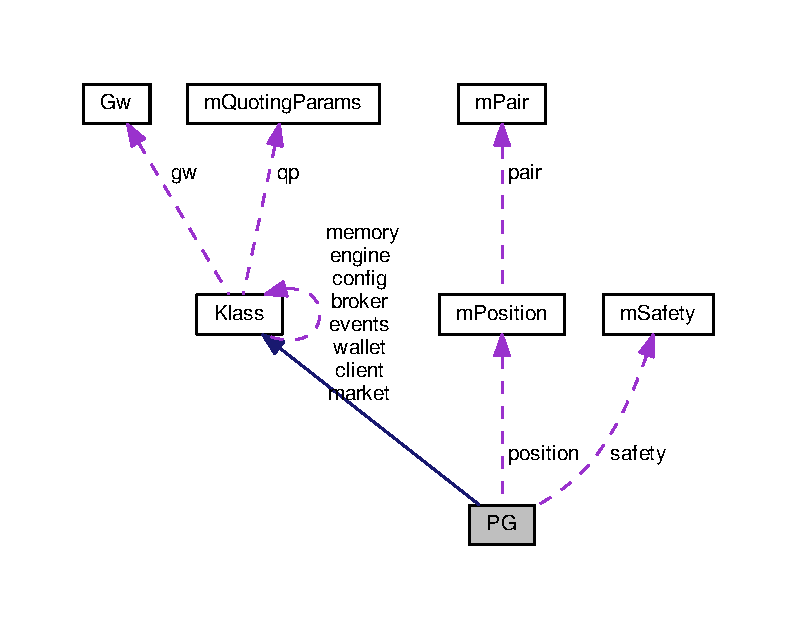
\includegraphics[width=350pt]{class_k_1_1_p_g__coll__graph}
\end{center}
\end{figure}
\subsection*{Public Member Functions}
\begin{DoxyCompactItemize}
\item 
void \hyperlink{class_k_1_1_p_g_af9636072c7613569127b37ecbfda5299}{calc\+Safety} ()
\end{DoxyCompactItemize}
\subsection*{Data Fields}
\begin{DoxyCompactItemize}
\item 
\hyperlink{struct_k_1_1m_position}{m\+Position} \hyperlink{class_k_1_1_p_g_afa6993a0243f938ec8a0b7a0ebc7a4d6}{position}
\item 
\hyperlink{struct_k_1_1m_safety}{m\+Safety} \hyperlink{class_k_1_1_p_g_a03dcb43533cb6cabba43716d9207b789}{safety}
\item 
\hyperlink{km_8h_ad4d00888c55a47a8a40ed8020d176086}{m\+Amount} \hyperlink{class_k_1_1_p_g_a41f7e688e22528d01be7373457b533c0}{target\+Base\+Position} = 0
\item 
\hyperlink{km_8h_ad4d00888c55a47a8a40ed8020d176086}{m\+Amount} \hyperlink{class_k_1_1_p_g_a158e860ce785d482b11cf81a6544cbd6}{position\+Divergence} = 0
\item 
string \hyperlink{class_k_1_1_p_g_af1d15671cf0f5d0d6c5ebac51f08bae1}{side\+A\+PR} = \char`\"{}\char`\"{}
\item 
function$<$ void()$>$ \hyperlink{class_k_1_1_p_g_a26ec2609ea48e49b3c4a482b6fe9fd38}{calc\+Target\+Base\+Pos}
\end{DoxyCompactItemize}
\subsection*{Protected Member Functions}
\begin{DoxyCompactItemize}
\item 
void \hyperlink{class_k_1_1_p_g_a78f61ac2dd03bcba8e09ca20cd7d68e3}{load} ()
\item 
void \hyperlink{class_k_1_1_p_g_aa9a0f090ee360e2a9f967200d30f4a22}{wait\+Data} ()
\item 
void \hyperlink{class_k_1_1_p_g_aa3f7b56799f5915cfbc902f6426c2bb2}{wait\+User} ()
\end{DoxyCompactItemize}
\subsection*{Additional Inherited Members}


\subsection{Detailed Description}


Definition at line 9 of file pg.\+h.



\subsection{Member Function Documentation}
\index{K\+::\+PG@{K\+::\+PG}!calc\+Safety@{calc\+Safety}}
\index{calc\+Safety@{calc\+Safety}!K\+::\+PG@{K\+::\+PG}}
\subsubsection[{\texorpdfstring{calc\+Safety()}{calcSafety()}}]{\setlength{\rightskip}{0pt plus 5cm}void calc\+Safety (
\begin{DoxyParamCaption}
{}
\end{DoxyParamCaption}
)\hspace{0.3cm}{\ttfamily [inline]}}\hypertarget{class_k_1_1_p_g_af9636072c7613569127b37ecbfda5299}{}\label{class_k_1_1_p_g_af9636072c7613569127b37ecbfda5299}


Definition at line 51 of file pg.\+h.

\index{K\+::\+PG@{K\+::\+PG}!load@{load}}
\index{load@{load}!K\+::\+PG@{K\+::\+PG}}
\subsubsection[{\texorpdfstring{load()}{load()}}]{\setlength{\rightskip}{0pt plus 5cm}void load (
\begin{DoxyParamCaption}
{}
\end{DoxyParamCaption}
)\hspace{0.3cm}{\ttfamily [inline]}, {\ttfamily [protected]}, {\ttfamily [virtual]}}\hypertarget{class_k_1_1_p_g_a78f61ac2dd03bcba8e09ca20cd7d68e3}{}\label{class_k_1_1_p_g_a78f61ac2dd03bcba8e09ca20cd7d68e3}


Reimplemented from \hyperlink{class_k_1_1_klass_a5588964fff1d1025245d134e159b60ee}{Klass}.



Definition at line 24 of file pg.\+h.

\index{K\+::\+PG@{K\+::\+PG}!wait\+Data@{wait\+Data}}
\index{wait\+Data@{wait\+Data}!K\+::\+PG@{K\+::\+PG}}
\subsubsection[{\texorpdfstring{wait\+Data()}{waitData()}}]{\setlength{\rightskip}{0pt plus 5cm}void wait\+Data (
\begin{DoxyParamCaption}
{}
\end{DoxyParamCaption}
)\hspace{0.3cm}{\ttfamily [inline]}, {\ttfamily [protected]}, {\ttfamily [virtual]}}\hypertarget{class_k_1_1_p_g_aa9a0f090ee360e2a9f967200d30f4a22}{}\label{class_k_1_1_p_g_aa9a0f090ee360e2a9f967200d30f4a22}


Reimplemented from \hyperlink{class_k_1_1_klass_a62a6bf36d7c8bec9dcf7af20c9d21d74}{Klass}.



Definition at line 37 of file pg.\+h.

\index{K\+::\+PG@{K\+::\+PG}!wait\+User@{wait\+User}}
\index{wait\+User@{wait\+User}!K\+::\+PG@{K\+::\+PG}}
\subsubsection[{\texorpdfstring{wait\+User()}{waitUser()}}]{\setlength{\rightskip}{0pt plus 5cm}void wait\+User (
\begin{DoxyParamCaption}
{}
\end{DoxyParamCaption}
)\hspace{0.3cm}{\ttfamily [inline]}, {\ttfamily [protected]}, {\ttfamily [virtual]}}\hypertarget{class_k_1_1_p_g_aa3f7b56799f5915cfbc902f6426c2bb2}{}\label{class_k_1_1_p_g_aa3f7b56799f5915cfbc902f6426c2bb2}


Reimplemented from \hyperlink{class_k_1_1_klass_af4f5201bed25a292d8a7f40470d83923}{Klass}.



Definition at line 45 of file pg.\+h.



\subsection{Field Documentation}
\index{K\+::\+PG@{K\+::\+PG}!calc\+Target\+Base\+Pos@{calc\+Target\+Base\+Pos}}
\index{calc\+Target\+Base\+Pos@{calc\+Target\+Base\+Pos}!K\+::\+PG@{K\+::\+PG}}
\subsubsection[{\texorpdfstring{calc\+Target\+Base\+Pos}{calcTargetBasePos}}]{\setlength{\rightskip}{0pt plus 5cm}function$<$void()$>$ calc\+Target\+Base\+Pos}\hypertarget{class_k_1_1_p_g_a26ec2609ea48e49b3c4a482b6fe9fd38}{}\label{class_k_1_1_p_g_a26ec2609ea48e49b3c4a482b6fe9fd38}
{\bfseries Initial value\+:}
\begin{DoxyCode}
= [&]() \{                  \hyperlink{ev_8h_ab96dcc845e16d51b3adbdb0cc9f39be1}{\_debugEvent\_}
        \textcolor{keywordflow}{if} (\hyperlink{class_k_1_1_p_g_afa6993a0243f938ec8a0b7a0ebc7a4d6}{position}.\hyperlink{struct_k_1_1m_position_a3f37b042a1e7cd4bd38fc564de81f0da}{empty}()) \textcolor{keywordflow}{return} ((SH*)\hyperlink{class_k_1_1_klass_a5819639653d62dde47c40c9d0c06f7ac}{screen})->logWar(\textcolor{stringliteral}{"PG"}, \textcolor{stringliteral}{"Unable to calculate
       TBP, missing wallet data"});
        \hyperlink{km_8h_ad4d00888c55a47a8a40ed8020d176086}{mAmount} baseValue = \hyperlink{class_k_1_1_p_g_afa6993a0243f938ec8a0b7a0ebc7a4d6}{position}.\hyperlink{struct_k_1_1m_position_adbb3d8b288708abaf509a644671fb442}{baseValue};
        \hyperlink{km_8h_ad4d00888c55a47a8a40ed8020d176086}{mAmount} next = \hyperlink{class_k_1_1_klass_a4554a7ffab1a73a5d43f13b9ac54ffb1}{qp}->\hyperlink{struct_k_1_1m_quoting_params_a57aeb3184bd7e2fa299e62ddd0e64273}{autoPositionMode} == 
      \hyperlink{namespace_k_a8708a45c314b4d4bb9e7221009ccee8aae1ba155a9f2e8c3be94020eef32a0301}{mAutoPositionMode::Manual}
          ? (\hyperlink{class_k_1_1_klass_a4554a7ffab1a73a5d43f13b9ac54ffb1}{qp}->\hyperlink{struct_k_1_1m_quoting_params_ac8404ecb555d84d2bef12ffae8b401b6}{percentageValues}
            ? \hyperlink{class_k_1_1_klass_a4554a7ffab1a73a5d43f13b9ac54ffb1}{qp}->\hyperlink{struct_k_1_1m_quoting_params_ae7a7b8af9caac8e6704751916b481c87}{targetBasePositionPercentage} * baseValue / 1e+2
            : \hyperlink{class_k_1_1_klass_a4554a7ffab1a73a5d43f13b9ac54ffb1}{qp}->\hyperlink{struct_k_1_1m_quoting_params_a41f7e688e22528d01be7373457b533c0}{targetBasePosition})
          : ((1 + ((MG*)\hyperlink{class_k_1_1_klass_a98dbde943a8c48f1f266b879e5409777}{market})->targetPosition) / 2) * baseValue;
        \textcolor{keywordflow}{if} (\hyperlink{class_k_1_1_p_g_a41f7e688e22528d01be7373457b533c0}{targetBasePosition} and abs(\hyperlink{class_k_1_1_p_g_a41f7e688e22528d01be7373457b533c0}{targetBasePosition} - next) < 1e-
      4 and sideAPR\_ == \hyperlink{class_k_1_1_p_g_af1d15671cf0f5d0d6c5ebac51f08bae1}{sideAPR}) \textcolor{keywordflow}{return};
        \hyperlink{class_k_1_1_p_g_a41f7e688e22528d01be7373457b533c0}{targetBasePosition} = next;
        sideAPR\_ = \hyperlink{class_k_1_1_p_g_af1d15671cf0f5d0d6c5ebac51f08bae1}{sideAPR};
        calcPDiv(baseValue);
        json k = \{\{\textcolor{stringliteral}{"tbp"}, \hyperlink{class_k_1_1_p_g_a41f7e688e22528d01be7373457b533c0}{targetBasePosition}\}, \{\textcolor{stringliteral}{"sideAPR"}, 
      \hyperlink{class_k_1_1_p_g_af1d15671cf0f5d0d6c5ebac51f08bae1}{sideAPR}\}, \{\textcolor{stringliteral}{"pDiv"}, \hyperlink{class_k_1_1_p_g_a158e860ce785d482b11cf81a6544cbd6}{positionDivergence} \}\};
        ((UI*)\hyperlink{class_k_1_1_klass_ad64d722352731ddedb64ba82179e0eaa}{client})->send(\hyperlink{namespace_k_a06e0333f0bcd3fc79835735bb9cda73dabe5c6be5c4decaf0b568f57bde929b6e}{mMatter::TargetBasePosition}, k);
        ((DB*)\hyperlink{class_k_1_1_klass_afe23c0cbde1ef3bc79fdd6e56f9c120a}{memory})->insert(\hyperlink{namespace_k_a06e0333f0bcd3fc79835735bb9cda73dabe5c6be5c4decaf0b568f57bde929b6e}{mMatter::TargetBasePosition}, k);
        \textcolor{keywordflow}{if} (!((CF*)\hyperlink{class_k_1_1_klass_a50e6a746d37cecad79ebeabcb5677722}{config})->argDebugWallet) \textcolor{keywordflow}{return};
        ((SH*)\hyperlink{class_k_1_1_klass_a5819639653d62dde47c40c9d0c06f7ac}{screen})->log(\textcolor{stringliteral}{"PG"}, \textcolor{keywordtype}{string}(\textcolor{stringliteral}{"TBP: "})
          + to\_string((\textcolor{keywordtype}{int})(\hyperlink{class_k_1_1_p_g_a41f7e688e22528d01be7373457b533c0}{targetBasePosition} / baseValue * 1e+2)) + \textcolor{stringliteral}{"% = "} + 
      \hyperlink{class_k_1_1_f_n_ae63dba2964cf9ff6d985f498dd9d0e57}{FN::str8}(\hyperlink{class_k_1_1_p_g_a41f7e688e22528d01be7373457b533c0}{targetBasePosition})
          + \textcolor{stringliteral}{" "} + \hyperlink{class_k_1_1_klass_a1cc87ecfd597953b3774a8e1fa4c25ec}{gw}->\hyperlink{class_k_1_1_gw_a88838a75375332fd734e38ba4d7d870c}{base} + \textcolor{stringliteral}{", pDiv: "}
          + to\_string((\textcolor{keywordtype}{int})(\hyperlink{class_k_1_1_p_g_a158e860ce785d482b11cf81a6544cbd6}{positionDivergence}  / baseValue * 1e+2)) + \textcolor{stringliteral}{"% = "} + 
      \hyperlink{class_k_1_1_f_n_ae63dba2964cf9ff6d985f498dd9d0e57}{FN::str8}(\hyperlink{class_k_1_1_p_g_a158e860ce785d482b11cf81a6544cbd6}{positionDivergence})
          + \textcolor{stringliteral}{" "} + \hyperlink{class_k_1_1_klass_a1cc87ecfd597953b3774a8e1fa4c25ec}{gw}->\hyperlink{class_k_1_1_gw_a88838a75375332fd734e38ba4d7d870c}{base});
      \}
\end{DoxyCode}


Definition at line 60 of file pg.\+h.

\index{K\+::\+PG@{K\+::\+PG}!position@{position}}
\index{position@{position}!K\+::\+PG@{K\+::\+PG}}
\subsubsection[{\texorpdfstring{position}{position}}]{\setlength{\rightskip}{0pt plus 5cm}{\bf m\+Position} position}\hypertarget{class_k_1_1_p_g_afa6993a0243f938ec8a0b7a0ebc7a4d6}{}\label{class_k_1_1_p_g_afa6993a0243f938ec8a0b7a0ebc7a4d6}


Definition at line 18 of file pg.\+h.

\index{K\+::\+PG@{K\+::\+PG}!position\+Divergence@{position\+Divergence}}
\index{position\+Divergence@{position\+Divergence}!K\+::\+PG@{K\+::\+PG}}
\subsubsection[{\texorpdfstring{position\+Divergence}{positionDivergence}}]{\setlength{\rightskip}{0pt plus 5cm}{\bf m\+Amount} position\+Divergence = 0}\hypertarget{class_k_1_1_p_g_a158e860ce785d482b11cf81a6544cbd6}{}\label{class_k_1_1_p_g_a158e860ce785d482b11cf81a6544cbd6}


Definition at line 21 of file pg.\+h.

\index{K\+::\+PG@{K\+::\+PG}!safety@{safety}}
\index{safety@{safety}!K\+::\+PG@{K\+::\+PG}}
\subsubsection[{\texorpdfstring{safety}{safety}}]{\setlength{\rightskip}{0pt plus 5cm}{\bf m\+Safety} safety}\hypertarget{class_k_1_1_p_g_a03dcb43533cb6cabba43716d9207b789}{}\label{class_k_1_1_p_g_a03dcb43533cb6cabba43716d9207b789}


Definition at line 19 of file pg.\+h.

\index{K\+::\+PG@{K\+::\+PG}!side\+A\+PR@{side\+A\+PR}}
\index{side\+A\+PR@{side\+A\+PR}!K\+::\+PG@{K\+::\+PG}}
\subsubsection[{\texorpdfstring{side\+A\+PR}{sideAPR}}]{\setlength{\rightskip}{0pt plus 5cm}string side\+A\+PR = \char`\"{}\char`\"{}}\hypertarget{class_k_1_1_p_g_af1d15671cf0f5d0d6c5ebac51f08bae1}{}\label{class_k_1_1_p_g_af1d15671cf0f5d0d6c5ebac51f08bae1}


Definition at line 22 of file pg.\+h.

\index{K\+::\+PG@{K\+::\+PG}!target\+Base\+Position@{target\+Base\+Position}}
\index{target\+Base\+Position@{target\+Base\+Position}!K\+::\+PG@{K\+::\+PG}}
\subsubsection[{\texorpdfstring{target\+Base\+Position}{targetBasePosition}}]{\setlength{\rightskip}{0pt plus 5cm}{\bf m\+Amount} target\+Base\+Position = 0}\hypertarget{class_k_1_1_p_g_a41f7e688e22528d01be7373457b533c0}{}\label{class_k_1_1_p_g_a41f7e688e22528d01be7373457b533c0}


Definition at line 20 of file pg.\+h.



The documentation for this class was generated from the following file\+:\begin{DoxyCompactItemize}
\item 
\hyperlink{pg_8h}{pg.\+h}\end{DoxyCompactItemize}

\hypertarget{class_k_1_1_q_e}{}\section{QE Class Reference}
\label{class_k_1_1_q_e}\index{QE@{QE}}


{\ttfamily \#include $<$qe.\+h$>$}



Inheritance diagram for QE\+:
\nopagebreak
\begin{figure}[H]
\begin{center}
\leavevmode
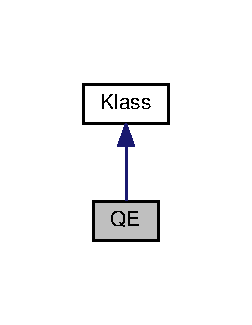
\includegraphics[width=121pt]{class_k_1_1_q_e__inherit__graph}
\end{center}
\end{figure}


Collaboration diagram for QE\+:
\nopagebreak
\begin{figure}[H]
\begin{center}
\leavevmode
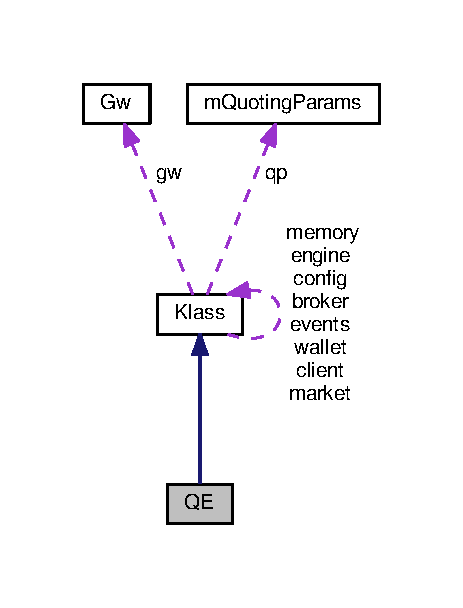
\includegraphics[width=222pt]{class_k_1_1_q_e__coll__graph}
\end{center}
\end{figure}
\subsection*{Public Member Functions}
\begin{DoxyCompactItemize}
\item 
void \hyperlink{class_k_1_1_q_e_ab13c95e3802af839eab18d5e6e11aa8e}{timer\+\_\+1s} ()
\end{DoxyCompactItemize}
\subsection*{Data Fields}
\begin{DoxyCompactItemize}
\item 
\hyperlink{namespace_k_a3da250819294c55d5728586148bfa19e}{m\+Connectivity} $\ast$ \hyperlink{class_k_1_1_q_e_a572945fdb3d861b6c685f6c5af9f1376}{gw\+Connected} = nullptr
\item 
\hyperlink{namespace_k_a3da250819294c55d5728586148bfa19e}{m\+Connectivity} $\ast$ \hyperlink{class_k_1_1_q_e_a6d9ed4a9793ac810eca371568ee912d3}{gw\+Connected\+Exchange} = nullptr
\item 
function$<$ void()$>$ \hyperlink{class_k_1_1_q_e_ad94592f5065d0e45c53b88f97036639a}{calc\+Quote\+After\+Saved\+Params}
\item 
function$<$ void()$>$ \hyperlink{class_k_1_1_q_e_a7fa74fffe521ea33c7a4c9deaa606994}{calc\+Quote}
\end{DoxyCompactItemize}
\subsection*{Protected Member Functions}
\begin{DoxyCompactItemize}
\item 
void \hyperlink{class_k_1_1_q_e_a78f61ac2dd03bcba8e09ca20cd7d68e3}{load} ()
\item 
void \hyperlink{class_k_1_1_q_e_aa9a0f090ee360e2a9f967200d30f4a22}{wait\+Data} ()
\item 
void \hyperlink{class_k_1_1_q_e_aa3f7b56799f5915cfbc902f6426c2bb2}{wait\+User} ()
\item 
void \hyperlink{class_k_1_1_q_e_a13a43e6d814de94978c515cb084873b1}{run} ()
\end{DoxyCompactItemize}
\subsection*{Additional Inherited Members}


\subsection{Detailed Description}


Definition at line 5 of file qe.\+h.



\subsection{Member Function Documentation}
\index{K\+::\+QE@{K\+::\+QE}!load@{load}}
\index{load@{load}!K\+::\+QE@{K\+::\+QE}}
\subsubsection[{\texorpdfstring{load()}{load()}}]{\setlength{\rightskip}{0pt plus 5cm}void load (
\begin{DoxyParamCaption}
{}
\end{DoxyParamCaption}
)\hspace{0.3cm}{\ttfamily [inline]}, {\ttfamily [protected]}, {\ttfamily [virtual]}}\hypertarget{class_k_1_1_q_e_a78f61ac2dd03bcba8e09ca20cd7d68e3}{}\label{class_k_1_1_q_e_a78f61ac2dd03bcba8e09ca20cd7d68e3}


Reimplemented from \hyperlink{class_k_1_1_klass_a5588964fff1d1025245d134e159b60ee}{Klass}.



Definition at line 16 of file qe.\+h.

\index{K\+::\+QE@{K\+::\+QE}!run@{run}}
\index{run@{run}!K\+::\+QE@{K\+::\+QE}}
\subsubsection[{\texorpdfstring{run()}{run()}}]{\setlength{\rightskip}{0pt plus 5cm}void run (
\begin{DoxyParamCaption}
{}
\end{DoxyParamCaption}
)\hspace{0.3cm}{\ttfamily [inline]}, {\ttfamily [protected]}, {\ttfamily [virtual]}}\hypertarget{class_k_1_1_q_e_a13a43e6d814de94978c515cb084873b1}{}\label{class_k_1_1_q_e_a13a43e6d814de94978c515cb084873b1}


Reimplemented from \hyperlink{class_k_1_1_klass_a72fcb26a14f6beb1c3fbace9ab3e7dbb}{Klass}.



Definition at line 33 of file qe.\+h.

\index{K\+::\+QE@{K\+::\+QE}!timer\+\_\+1s@{timer\+\_\+1s}}
\index{timer\+\_\+1s@{timer\+\_\+1s}!K\+::\+QE@{K\+::\+QE}}
\subsubsection[{\texorpdfstring{timer\+\_\+1s()}{timer_1s()}}]{\setlength{\rightskip}{0pt plus 5cm}void timer\+\_\+1s (
\begin{DoxyParamCaption}
{}
\end{DoxyParamCaption}
)\hspace{0.3cm}{\ttfamily [inline]}}\hypertarget{class_k_1_1_q_e_ab13c95e3802af839eab18d5e6e11aa8e}{}\label{class_k_1_1_q_e_ab13c95e3802af839eab18d5e6e11aa8e}


Definition at line 39 of file qe.\+h.

\index{K\+::\+QE@{K\+::\+QE}!wait\+Data@{wait\+Data}}
\index{wait\+Data@{wait\+Data}!K\+::\+QE@{K\+::\+QE}}
\subsubsection[{\texorpdfstring{wait\+Data()}{waitData()}}]{\setlength{\rightskip}{0pt plus 5cm}void wait\+Data (
\begin{DoxyParamCaption}
{}
\end{DoxyParamCaption}
)\hspace{0.3cm}{\ttfamily [inline]}, {\ttfamily [protected]}, {\ttfamily [virtual]}}\hypertarget{class_k_1_1_q_e_aa9a0f090ee360e2a9f967200d30f4a22}{}\label{class_k_1_1_q_e_aa9a0f090ee360e2a9f967200d30f4a22}


Reimplemented from \hyperlink{class_k_1_1_klass_a62a6bf36d7c8bec9dcf7af20c9d21d74}{Klass}.



Definition at line 26 of file qe.\+h.

\index{K\+::\+QE@{K\+::\+QE}!wait\+User@{wait\+User}}
\index{wait\+User@{wait\+User}!K\+::\+QE@{K\+::\+QE}}
\subsubsection[{\texorpdfstring{wait\+User()}{waitUser()}}]{\setlength{\rightskip}{0pt plus 5cm}void wait\+User (
\begin{DoxyParamCaption}
{}
\end{DoxyParamCaption}
)\hspace{0.3cm}{\ttfamily [inline]}, {\ttfamily [protected]}, {\ttfamily [virtual]}}\hypertarget{class_k_1_1_q_e_aa3f7b56799f5915cfbc902f6426c2bb2}{}\label{class_k_1_1_q_e_aa3f7b56799f5915cfbc902f6426c2bb2}


Reimplemented from \hyperlink{class_k_1_1_klass_af4f5201bed25a292d8a7f40470d83923}{Klass}.



Definition at line 30 of file qe.\+h.



\subsection{Field Documentation}
\index{K\+::\+QE@{K\+::\+QE}!calc\+Quote@{calc\+Quote}}
\index{calc\+Quote@{calc\+Quote}!K\+::\+QE@{K\+::\+QE}}
\subsubsection[{\texorpdfstring{calc\+Quote}{calcQuote}}]{\setlength{\rightskip}{0pt plus 5cm}function$<$void()$>$ calc\+Quote}\hypertarget{class_k_1_1_q_e_a7fa74fffe521ea33c7a4c9deaa606994}{}\label{class_k_1_1_q_e_a7fa74fffe521ea33c7a4c9deaa606994}
{\bfseries Initial value\+:}
\begin{DoxyCode}
= [&]() \{                          \hyperlink{ev_8h_ab96dcc845e16d51b3adbdb0cc9f39be1}{\_debugEvent\_}
        bidStatus = \hyperlink{namespace_k_a76b6774ff9252e574d375a353ecf6736afe155956e8f33e5cffa82cc86a36afbd}{mQuoteState::MissingData};
        askStatus = \hyperlink{namespace_k_a76b6774ff9252e574d375a353ecf6736afe155956e8f33e5cffa82cc86a36afbd}{mQuoteState::MissingData};
        \textcolor{keywordflow}{if} (!*\hyperlink{class_k_1_1_q_e_a6d9ed4a9793ac810eca371568ee912d3}{gwConnectedExchange}) \{
          bidStatus = \hyperlink{namespace_k_a3da250819294c55d5728586148bfa19eaef70e46fd3bbc21e3e1f0b6815e750c0}{mQuoteState::Disconnected};
          askStatus = \hyperlink{namespace_k_a3da250819294c55d5728586148bfa19eaef70e46fd3bbc21e3e1f0b6815e750c0}{mQuoteState::Disconnected};
        \} \textcolor{keywordflow}{else} \textcolor{keywordflow}{if} (((MG*)\hyperlink{class_k_1_1_klass_a98dbde943a8c48f1f266b879e5409777}{market})->fairValue
          and !((MG*)\hyperlink{class_k_1_1_klass_a98dbde943a8c48f1f266b879e5409777}{market})->levels.empty()
          and !((PG*)\hyperlink{class_k_1_1_klass_a5943d9c958085108c746fdc756c7aad3}{wallet})->position.empty()
          and !((PG*)\hyperlink{class_k_1_1_klass_a5943d9c958085108c746fdc756c7aad3}{wallet})->safety.empty()
        ) \{
          \textcolor{keywordflow}{if} (!*\hyperlink{class_k_1_1_q_e_a572945fdb3d861b6c685f6c5af9f1376}{gwConnected}) \{
            bidStatus = \hyperlink{namespace_k_a76b6774ff9252e574d375a353ecf6736a152243c591927afa2121aea8911cccd2}{mQuoteState::DisabledQuotes};
            askStatus = \hyperlink{namespace_k_a76b6774ff9252e574d375a353ecf6736a152243c591927afa2121aea8911cccd2}{mQuoteState::DisabledQuotes};
            stopAllQuotes(\hyperlink{namespace_k_a0b7d0fa0ffc9f87da1d6499cbcee7e94a130c5b3473c57faa76e2a1c54e26f88e}{mSide::Both});
          \} \textcolor{keywordflow}{else} \{
            bidStatus = \hyperlink{namespace_k_a76b6774ff9252e574d375a353ecf6736aa6dd615eded3f865e7f58d646d053222}{mQuoteState::UnknownHeld};
            askStatus = \hyperlink{namespace_k_a76b6774ff9252e574d375a353ecf6736aa6dd615eded3f865e7f58d646d053222}{mQuoteState::UnknownHeld};
            sendQuoteToAPI();
          \}
        \}
        sendStatusToUI();
      \}
\end{DoxyCode}


Definition at line 54 of file qe.\+h.

\index{K\+::\+QE@{K\+::\+QE}!calc\+Quote\+After\+Saved\+Params@{calc\+Quote\+After\+Saved\+Params}}
\index{calc\+Quote\+After\+Saved\+Params@{calc\+Quote\+After\+Saved\+Params}!K\+::\+QE@{K\+::\+QE}}
\subsubsection[{\texorpdfstring{calc\+Quote\+After\+Saved\+Params}{calcQuoteAfterSavedParams}}]{\setlength{\rightskip}{0pt plus 5cm}function$<$void()$>$ calc\+Quote\+After\+Saved\+Params}\hypertarget{class_k_1_1_q_e_ad94592f5065d0e45c53b88f97036639a}{}\label{class_k_1_1_q_e_ad94592f5065d0e45c53b88f97036639a}
{\bfseries Initial value\+:}
\begin{DoxyCode}
= [&]() \{
        findMode(\textcolor{stringliteral}{"saved"});
        ((MG*)\hyperlink{class_k_1_1_klass_a98dbde943a8c48f1f266b879e5409777}{market})->calcFairValue();
        ((PG*)\hyperlink{class_k_1_1_klass_a5943d9c958085108c746fdc756c7aad3}{wallet})->calcTargetBasePos();
        ((PG*)\hyperlink{class_k_1_1_klass_a5943d9c958085108c746fdc756c7aad3}{wallet})->calcSafety();
        ((MG*)\hyperlink{class_k_1_1_klass_a98dbde943a8c48f1f266b879e5409777}{market})->calcEwmaHistory();
        \hyperlink{class_k_1_1_q_e_a7fa74fffe521ea33c7a4c9deaa606994}{calcQuote}();
      \}
\end{DoxyCode}


Definition at line 46 of file qe.\+h.

\index{K\+::\+QE@{K\+::\+QE}!gw\+Connected@{gw\+Connected}}
\index{gw\+Connected@{gw\+Connected}!K\+::\+QE@{K\+::\+QE}}
\subsubsection[{\texorpdfstring{gw\+Connected}{gwConnected}}]{\setlength{\rightskip}{0pt plus 5cm}{\bf m\+Connectivity}$\ast$ gw\+Connected = nullptr}\hypertarget{class_k_1_1_q_e_a572945fdb3d861b6c685f6c5af9f1376}{}\label{class_k_1_1_q_e_a572945fdb3d861b6c685f6c5af9f1376}


Definition at line 13 of file qe.\+h.

\index{K\+::\+QE@{K\+::\+QE}!gw\+Connected\+Exchange@{gw\+Connected\+Exchange}}
\index{gw\+Connected\+Exchange@{gw\+Connected\+Exchange}!K\+::\+QE@{K\+::\+QE}}
\subsubsection[{\texorpdfstring{gw\+Connected\+Exchange}{gwConnectedExchange}}]{\setlength{\rightskip}{0pt plus 5cm}{\bf m\+Connectivity} $\ast$ gw\+Connected\+Exchange = nullptr}\hypertarget{class_k_1_1_q_e_a6d9ed4a9793ac810eca371568ee912d3}{}\label{class_k_1_1_q_e_a6d9ed4a9793ac810eca371568ee912d3}


Definition at line 14 of file qe.\+h.



The documentation for this class was generated from the following file\+:\begin{DoxyCompactItemize}
\item 
\hyperlink{qe_8h}{qe.\+h}\end{DoxyCompactItemize}

\hypertarget{class_k_1_1_q_p}{}\section{QP Class Reference}
\label{class_k_1_1_q_p}\index{QP@{QP}}


{\ttfamily \#include $<$qp.\+h$>$}



Inheritance diagram for QP\+:
\nopagebreak
\begin{figure}[H]
\begin{center}
\leavevmode
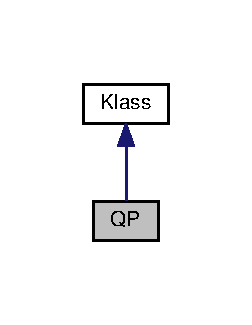
\includegraphics[width=121pt]{class_k_1_1_q_p__inherit__graph}
\end{center}
\end{figure}


Collaboration diagram for QP\+:
\nopagebreak
\begin{figure}[H]
\begin{center}
\leavevmode
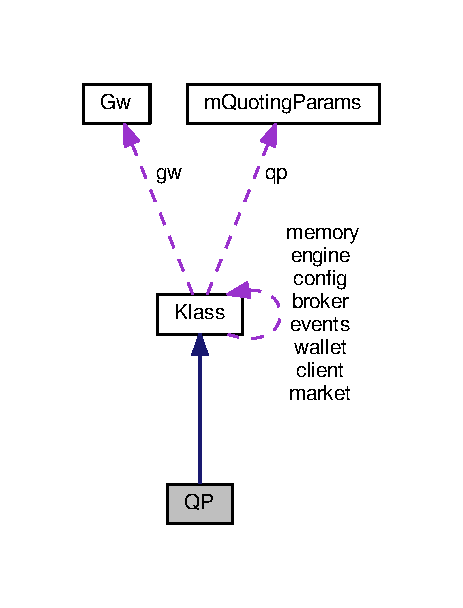
\includegraphics[width=222pt]{class_k_1_1_q_p__coll__graph}
\end{center}
\end{figure}
\subsection*{Protected Member Functions}
\begin{DoxyCompactItemize}
\item 
void \hyperlink{class_k_1_1_q_p_a78f61ac2dd03bcba8e09ca20cd7d68e3}{load} ()
\item 
void \hyperlink{class_k_1_1_q_p_aa3f7b56799f5915cfbc902f6426c2bb2}{wait\+User} ()
\item 
void \hyperlink{class_k_1_1_q_p_a13a43e6d814de94978c515cb084873b1}{run} ()
\end{DoxyCompactItemize}
\subsection*{Additional Inherited Members}


\subsection{Detailed Description}


Definition at line 5 of file qp.\+h.



\subsection{Member Function Documentation}
\index{K\+::\+QP@{K\+::\+QP}!load@{load}}
\index{load@{load}!K\+::\+QP@{K\+::\+QP}}
\subsubsection[{\texorpdfstring{load()}{load()}}]{\setlength{\rightskip}{0pt plus 5cm}void load (
\begin{DoxyParamCaption}
{}
\end{DoxyParamCaption}
)\hspace{0.3cm}{\ttfamily [inline]}, {\ttfamily [protected]}, {\ttfamily [virtual]}}\hypertarget{class_k_1_1_q_p_a78f61ac2dd03bcba8e09ca20cd7d68e3}{}\label{class_k_1_1_q_p_a78f61ac2dd03bcba8e09ca20cd7d68e3}


Reimplemented from \hyperlink{class_k_1_1_klass_a5588964fff1d1025245d134e159b60ee}{Klass}.



Definition at line 7 of file qp.\+h.

\index{K\+::\+QP@{K\+::\+QP}!run@{run}}
\index{run@{run}!K\+::\+QP@{K\+::\+QP}}
\subsubsection[{\texorpdfstring{run()}{run()}}]{\setlength{\rightskip}{0pt plus 5cm}void run (
\begin{DoxyParamCaption}
{}
\end{DoxyParamCaption}
)\hspace{0.3cm}{\ttfamily [inline]}, {\ttfamily [protected]}, {\ttfamily [virtual]}}\hypertarget{class_k_1_1_q_p_a13a43e6d814de94978c515cb084873b1}{}\label{class_k_1_1_q_p_a13a43e6d814de94978c515cb084873b1}


Reimplemented from \hyperlink{class_k_1_1_klass_a72fcb26a14f6beb1c3fbace9ab3e7dbb}{Klass}.



Definition at line 17 of file qp.\+h.

\index{K\+::\+QP@{K\+::\+QP}!wait\+User@{wait\+User}}
\index{wait\+User@{wait\+User}!K\+::\+QP@{K\+::\+QP}}
\subsubsection[{\texorpdfstring{wait\+User()}{waitUser()}}]{\setlength{\rightskip}{0pt plus 5cm}void wait\+User (
\begin{DoxyParamCaption}
{}
\end{DoxyParamCaption}
)\hspace{0.3cm}{\ttfamily [inline]}, {\ttfamily [protected]}, {\ttfamily [virtual]}}\hypertarget{class_k_1_1_q_p_aa3f7b56799f5915cfbc902f6426c2bb2}{}\label{class_k_1_1_q_p_aa3f7b56799f5915cfbc902f6426c2bb2}


Reimplemented from \hyperlink{class_k_1_1_klass_af4f5201bed25a292d8a7f40470d83923}{Klass}.



Definition at line 13 of file qp.\+h.



The documentation for this class was generated from the following file\+:\begin{DoxyCompactItemize}
\item 
\hyperlink{qp_8h}{qp.\+h}\end{DoxyCompactItemize}

\hypertarget{class_k_1_1_s_h}{}\section{SH Class Reference}
\label{class_k_1_1_s_h}\index{SH@{SH}}


{\ttfamily \#include $<$sh.\+h$>$}

\subsection*{Public Member Functions}
\begin{DoxyCompactItemize}
\item 
\hyperlink{class_k_1_1_s_h_a318dc7a3f5064dac8e50e5d9fbd5d75f}{SH} ()
\item 
void \hyperlink{class_k_1_1_s_h_abacd4501fa9314b249f770765816dce5}{config} (string base\+\_\+, string quote\+\_\+, string arg\+Exchange, int arg\+Colors, int arg\+Port, int arg\+Naked)
\item 
void \hyperlink{class_k_1_1_s_h_a4c6bd9d7e5cc908ef96085609e455cb1}{pressme} (\hyperlink{namespace_k_a211862d8b09ec46a051464b6859c1306}{m\+Hotkey} ch, function$<$ void()$>$ $\ast$fn)
\item 
void \hyperlink{class_k_1_1_s_h_a2463a3acef2df4c951ce942a3229e44e}{quit} ()
\item 
int \hyperlink{class_k_1_1_s_h_a4c49d97d050be83fa5908a03c8c47c8a}{error} (string k, string s, bool reboot=false)
\item 
void \hyperlink{class_k_1_1_s_h_ae8fa6fc69497d85bcf25571f2f80f353}{wait\+For\+User} ()
\item 
string \hyperlink{class_k_1_1_s_h_a9467c6fc12388f8513d2f21f76bb7dc7}{stamp} ()
\item 
void \hyperlink{class_k_1_1_s_h_aa6ff36d9cf9124487791c66fe0f121e7}{log\+War} (string k, string s)
\item 
void \hyperlink{class_k_1_1_s_h_a81e184501800070f574e7b688069c3ec}{log\+Err} (string k, string s, string m=\char`\"{} Errrror\+: \char`\"{})
\item 
void \hyperlink{class_k_1_1_s_h_af67052c37f765ca542764f5fcfdde593}{log\+DB} (string k)
\item 
void \hyperlink{class_k_1_1_s_h_aca26ec816d45509907350a56b57ea869}{log\+UI} ()
\item 
void \hyperlink{class_k_1_1_s_h_aeea74b282180b4d73d9855920edecc7f}{log\+U\+Isess} (int k, string s)
\item 
void \hyperlink{class_k_1_1_s_h_a09145551996ba5f25fb67280967aef90}{log\+Ver} (string k, int c)
\item 
void \hyperlink{class_k_1_1_s_h_a50fa1ebfccaac1a37b97b499780a4d30}{log} (\hyperlink{struct_k_1_1m_trade}{m\+Trade} k, string e)
\item 
void \hyperlink{class_k_1_1_s_h_a05d165fd99c6a9407040879a506bcf94}{log} (string k, string s, string v)
\item 
void \hyperlink{class_k_1_1_s_h_ac768cf60d7151187490fb98888116fbf}{log} (string k, string s)
\item 
void \hyperlink{class_k_1_1_s_h_a81f63afb8bf5d2129520b9d83a8aae45}{log} (string k, int c=C\+O\+L\+O\+R\+\_\+\+W\+H\+I\+TE, bool b=false)
\item 
void \hyperlink{class_k_1_1_s_h_a56dbc67f7f81955c835dee9802bc6d90}{log} (const map$<$ \hyperlink{km_8h_a23233b27e494114073abc4d494b05626}{m\+Rand\+Id}, \hyperlink{struct_k_1_1m_order}{m\+Order} $>$ \&orders, bool working)
\item 
void \hyperlink{class_k_1_1_s_h_a5be6e66b940b986413db423ab7df1cd2}{log} (const \hyperlink{struct_k_1_1m_position}{m\+Position} \&pos)
\item 
void \hyperlink{class_k_1_1_s_h_ac7b5f65dd2a0c700f7ab8c39ff6c5963}{log} (double fv)
\item 
void \hyperlink{class_k_1_1_s_h_a5f2e190b8261a98c97c2ea4e86670d54}{refresh} ()
\end{DoxyCompactItemize}
\subsection*{Static Public Member Functions}
\begin{DoxyCompactItemize}
\item 
static string \hyperlink{class_k_1_1_s_h_abb2930f405f8983fca3bab0e1d505a85}{changelog} ()
\end{DoxyCompactItemize}
\subsection*{Data Fields}
\begin{DoxyCompactItemize}
\item 
string \hyperlink{class_k_1_1_s_h_aeb72b6e20d3a581dcdede91beb824d9f}{protocol} = \char`\"{}H\+T\+TP\char`\"{}
\item 
\hyperlink{namespace_k_a3da250819294c55d5728586148bfa19e}{m\+Connectivity} $\ast$ \hyperlink{class_k_1_1_s_h_a572945fdb3d861b6c685f6c5af9f1376}{gw\+Connected} = nullptr
\item 
\hyperlink{namespace_k_a3da250819294c55d5728586148bfa19e}{m\+Connectivity} $\ast$ \hyperlink{class_k_1_1_s_h_a6d9ed4a9793ac810eca371568ee912d3}{gw\+Connected\+Exchange} = nullptr
\end{DoxyCompactItemize}


\subsection{Detailed Description}


Definition at line 13 of file sh.\+h.



\subsection{Constructor \& Destructor Documentation}
\index{K\+::\+SH@{K\+::\+SH}!SH@{SH}}
\index{SH@{SH}!K\+::\+SH@{K\+::\+SH}}
\subsubsection[{\texorpdfstring{S\+H()}{SH()}}]{\setlength{\rightskip}{0pt plus 5cm}{\bf SH} (
\begin{DoxyParamCaption}
{}
\end{DoxyParamCaption}
)\hspace{0.3cm}{\ttfamily [inline]}}\hypertarget{class_k_1_1_s_h_a318dc7a3f5064dac8e50e5d9fbd5d75f}{}\label{class_k_1_1_s_h_a318dc7a3f5064dac8e50e5d9fbd5d75f}


Definition at line 40 of file sh.\+h.



\subsection{Member Function Documentation}
\index{K\+::\+SH@{K\+::\+SH}!changelog@{changelog}}
\index{changelog@{changelog}!K\+::\+SH@{K\+::\+SH}}
\subsubsection[{\texorpdfstring{changelog()}{changelog()}}]{\setlength{\rightskip}{0pt plus 5cm}static string changelog (
\begin{DoxyParamCaption}
{}
\end{DoxyParamCaption}
)\hspace{0.3cm}{\ttfamily [inline]}, {\ttfamily [static]}}\hypertarget{class_k_1_1_s_h_abb2930f405f8983fca3bab0e1d505a85}{}\label{class_k_1_1_s_h_abb2930f405f8983fca3bab0e1d505a85}


Definition at line 82 of file sh.\+h.

\index{K\+::\+SH@{K\+::\+SH}!config@{config}}
\index{config@{config}!K\+::\+SH@{K\+::\+SH}}
\subsubsection[{\texorpdfstring{config(string base\+\_\+, string quote\+\_\+, string arg\+Exchange, int arg\+Colors, int arg\+Port, int arg\+Naked)}{config(string base_, string quote_, string argExchange, int argColors, int argPort, int argNaked)}}]{\setlength{\rightskip}{0pt plus 5cm}void config (
\begin{DoxyParamCaption}
\item[{string}]{base\+\_\+, }
\item[{string}]{quote\+\_\+, }
\item[{string}]{arg\+Exchange, }
\item[{int}]{arg\+Colors, }
\item[{int}]{arg\+Port, }
\item[{int}]{arg\+Naked}
\end{DoxyParamCaption}
)\hspace{0.3cm}{\ttfamily [inline]}}\hypertarget{class_k_1_1_s_h_abacd4501fa9314b249f770765816dce5}{}\label{class_k_1_1_s_h_abacd4501fa9314b249f770765816dce5}


Definition at line 50 of file sh.\+h.

\index{K\+::\+SH@{K\+::\+SH}!error@{error}}
\index{error@{error}!K\+::\+SH@{K\+::\+SH}}
\subsubsection[{\texorpdfstring{error(string k, string s, bool reboot=false)}{error(string k, string s, bool reboot=false)}}]{\setlength{\rightskip}{0pt plus 5cm}int error (
\begin{DoxyParamCaption}
\item[{string}]{k, }
\item[{string}]{s, }
\item[{bool}]{reboot = {\ttfamily false}}
\end{DoxyParamCaption}
)\hspace{0.3cm}{\ttfamily [inline]}}\hypertarget{class_k_1_1_s_h_a4c49d97d050be83fa5908a03c8c47c8a}{}\label{class_k_1_1_s_h_a4c49d97d050be83fa5908a03c8c47c8a}


Definition at line 95 of file sh.\+h.

\index{K\+::\+SH@{K\+::\+SH}!log@{log}}
\index{log@{log}!K\+::\+SH@{K\+::\+SH}}
\subsubsection[{\texorpdfstring{log(m\+Trade k, string e)}{log(mTrade k, string e)}}]{\setlength{\rightskip}{0pt plus 5cm}void log (
\begin{DoxyParamCaption}
\item[{{\bf m\+Trade}}]{k, }
\item[{string}]{e}
\end{DoxyParamCaption}
)\hspace{0.3cm}{\ttfamily [inline]}}\hypertarget{class_k_1_1_s_h_a50fa1ebfccaac1a37b97b499780a4d30}{}\label{class_k_1_1_s_h_a50fa1ebfccaac1a37b97b499780a4d30}


Definition at line 238 of file sh.\+h.

\index{K\+::\+SH@{K\+::\+SH}!log@{log}}
\index{log@{log}!K\+::\+SH@{K\+::\+SH}}
\subsubsection[{\texorpdfstring{log(string k, string s, string v)}{log(string k, string s, string v)}}]{\setlength{\rightskip}{0pt plus 5cm}void log (
\begin{DoxyParamCaption}
\item[{string}]{k, }
\item[{string}]{s, }
\item[{string}]{v}
\end{DoxyParamCaption}
)\hspace{0.3cm}{\ttfamily [inline]}}\hypertarget{class_k_1_1_s_h_a05d165fd99c6a9407040879a506bcf94}{}\label{class_k_1_1_s_h_a05d165fd99c6a9407040879a506bcf94}


Definition at line 261 of file sh.\+h.

\index{K\+::\+SH@{K\+::\+SH}!log@{log}}
\index{log@{log}!K\+::\+SH@{K\+::\+SH}}
\subsubsection[{\texorpdfstring{log(string k, string s)}{log(string k, string s)}}]{\setlength{\rightskip}{0pt plus 5cm}void log (
\begin{DoxyParamCaption}
\item[{string}]{k, }
\item[{string}]{s}
\end{DoxyParamCaption}
)\hspace{0.3cm}{\ttfamily [inline]}}\hypertarget{class_k_1_1_s_h_ac768cf60d7151187490fb98888116fbf}{}\label{class_k_1_1_s_h_ac768cf60d7151187490fb98888116fbf}


Definition at line 282 of file sh.\+h.

\index{K\+::\+SH@{K\+::\+SH}!log@{log}}
\index{log@{log}!K\+::\+SH@{K\+::\+SH}}
\subsubsection[{\texorpdfstring{log(string k, int c=\+C\+O\+L\+O\+R\+\_\+\+W\+H\+I\+T\+E, bool b=false)}{log(string k, int c=COLOR_WHITE, bool b=false)}}]{\setlength{\rightskip}{0pt plus 5cm}void log (
\begin{DoxyParamCaption}
\item[{string}]{k, }
\item[{int}]{c = {\ttfamily COLOR\+\_\+WHITE}, }
\item[{bool}]{b = {\ttfamily false}}
\end{DoxyParamCaption}
)\hspace{0.3cm}{\ttfamily [inline]}}\hypertarget{class_k_1_1_s_h_a81f63afb8bf5d2129520b9d83a8aae45}{}\label{class_k_1_1_s_h_a81f63afb8bf5d2129520b9d83a8aae45}


Definition at line 297 of file sh.\+h.

\index{K\+::\+SH@{K\+::\+SH}!log@{log}}
\index{log@{log}!K\+::\+SH@{K\+::\+SH}}
\subsubsection[{\texorpdfstring{log(const map$<$ m\+Rand\+Id, m\+Order $>$ \&orders, bool working)}{log(const map< mRandId, mOrder > &orders, bool working)}}]{\setlength{\rightskip}{0pt plus 5cm}void log (
\begin{DoxyParamCaption}
\item[{const map$<$ {\bf m\+Rand\+Id}, {\bf m\+Order} $>$ \&}]{orders, }
\item[{bool}]{working}
\end{DoxyParamCaption}
)\hspace{0.3cm}{\ttfamily [inline]}}\hypertarget{class_k_1_1_s_h_a56dbc67f7f81955c835dee9802bc6d90}{}\label{class_k_1_1_s_h_a56dbc67f7f81955c835dee9802bc6d90}


Definition at line 310 of file sh.\+h.

\index{K\+::\+SH@{K\+::\+SH}!log@{log}}
\index{log@{log}!K\+::\+SH@{K\+::\+SH}}
\subsubsection[{\texorpdfstring{log(const m\+Position \&pos)}{log(const mPosition &pos)}}]{\setlength{\rightskip}{0pt plus 5cm}void log (
\begin{DoxyParamCaption}
\item[{const {\bf m\+Position} \&}]{pos}
\end{DoxyParamCaption}
)\hspace{0.3cm}{\ttfamily [inline]}}\hypertarget{class_k_1_1_s_h_a5be6e66b940b986413db423ab7df1cd2}{}\label{class_k_1_1_s_h_a5be6e66b940b986413db423ab7df1cd2}


Definition at line 319 of file sh.\+h.

\index{K\+::\+SH@{K\+::\+SH}!log@{log}}
\index{log@{log}!K\+::\+SH@{K\+::\+SH}}
\subsubsection[{\texorpdfstring{log(double fv)}{log(double fv)}}]{\setlength{\rightskip}{0pt plus 5cm}void log (
\begin{DoxyParamCaption}
\item[{double}]{fv}
\end{DoxyParamCaption}
)\hspace{0.3cm}{\ttfamily [inline]}}\hypertarget{class_k_1_1_s_h_ac7b5f65dd2a0c700f7ab8c39ff6c5963}{}\label{class_k_1_1_s_h_ac7b5f65dd2a0c700f7ab8c39ff6c5963}


Definition at line 329 of file sh.\+h.

\index{K\+::\+SH@{K\+::\+SH}!log\+DB@{log\+DB}}
\index{log\+DB@{log\+DB}!K\+::\+SH@{K\+::\+SH}}
\subsubsection[{\texorpdfstring{log\+D\+B(string k)}{logDB(string k)}}]{\setlength{\rightskip}{0pt plus 5cm}void log\+DB (
\begin{DoxyParamCaption}
\item[{string}]{k}
\end{DoxyParamCaption}
)\hspace{0.3cm}{\ttfamily [inline]}}\hypertarget{class_k_1_1_s_h_af67052c37f765ca542764f5fcfdde593}{}\label{class_k_1_1_s_h_af67052c37f765ca542764f5fcfdde593}


Definition at line 161 of file sh.\+h.

\index{K\+::\+SH@{K\+::\+SH}!log\+Err@{log\+Err}}
\index{log\+Err@{log\+Err}!K\+::\+SH@{K\+::\+SH}}
\subsubsection[{\texorpdfstring{log\+Err(string k, string s, string m="" Errrror\+: "")}{logErr(string k, string s, string m=" Errrror: ")}}]{\setlength{\rightskip}{0pt plus 5cm}void log\+Err (
\begin{DoxyParamCaption}
\item[{string}]{k, }
\item[{string}]{s, }
\item[{string}]{m = {\ttfamily \char`\"{}~Errrror\+:~\char`\"{}}}
\end{DoxyParamCaption}
)\hspace{0.3cm}{\ttfamily [inline]}}\hypertarget{class_k_1_1_s_h_a81e184501800070f574e7b688069c3ec}{}\label{class_k_1_1_s_h_a81e184501800070f574e7b688069c3ec}


Definition at line 140 of file sh.\+h.

\index{K\+::\+SH@{K\+::\+SH}!log\+UI@{log\+UI}}
\index{log\+UI@{log\+UI}!K\+::\+SH@{K\+::\+SH}}
\subsubsection[{\texorpdfstring{log\+U\+I()}{logUI()}}]{\setlength{\rightskip}{0pt plus 5cm}void log\+UI (
\begin{DoxyParamCaption}
{}
\end{DoxyParamCaption}
)\hspace{0.3cm}{\ttfamily [inline]}}\hypertarget{class_k_1_1_s_h_aca26ec816d45509907350a56b57ea869}{}\label{class_k_1_1_s_h_aca26ec816d45509907350a56b57ea869}


Definition at line 181 of file sh.\+h.

\index{K\+::\+SH@{K\+::\+SH}!log\+U\+Isess@{log\+U\+Isess}}
\index{log\+U\+Isess@{log\+U\+Isess}!K\+::\+SH@{K\+::\+SH}}
\subsubsection[{\texorpdfstring{log\+U\+Isess(int k, string s)}{logUIsess(int k, string s)}}]{\setlength{\rightskip}{0pt plus 5cm}void log\+U\+Isess (
\begin{DoxyParamCaption}
\item[{int}]{k, }
\item[{string}]{s}
\end{DoxyParamCaption}
)\hspace{0.3cm}{\ttfamily [inline]}}\hypertarget{class_k_1_1_s_h_aeea74b282180b4d73d9855920edecc7f}{}\label{class_k_1_1_s_h_aeea74b282180b4d73d9855920edecc7f}


Definition at line 208 of file sh.\+h.

\index{K\+::\+SH@{K\+::\+SH}!log\+Ver@{log\+Ver}}
\index{log\+Ver@{log\+Ver}!K\+::\+SH@{K\+::\+SH}}
\subsubsection[{\texorpdfstring{log\+Ver(string k, int c)}{logVer(string k, int c)}}]{\setlength{\rightskip}{0pt plus 5cm}void log\+Ver (
\begin{DoxyParamCaption}
\item[{string}]{k, }
\item[{int}]{c}
\end{DoxyParamCaption}
)\hspace{0.3cm}{\ttfamily [inline]}}\hypertarget{class_k_1_1_s_h_a09145551996ba5f25fb67280967aef90}{}\label{class_k_1_1_s_h_a09145551996ba5f25fb67280967aef90}


Definition at line 235 of file sh.\+h.

\index{K\+::\+SH@{K\+::\+SH}!log\+War@{log\+War}}
\index{log\+War@{log\+War}!K\+::\+SH@{K\+::\+SH}}
\subsubsection[{\texorpdfstring{log\+War(string k, string s)}{logWar(string k, string s)}}]{\setlength{\rightskip}{0pt plus 5cm}void log\+War (
\begin{DoxyParamCaption}
\item[{string}]{k, }
\item[{string}]{s}
\end{DoxyParamCaption}
)\hspace{0.3cm}{\ttfamily [inline]}}\hypertarget{class_k_1_1_s_h_aa6ff36d9cf9124487791c66fe0f121e7}{}\label{class_k_1_1_s_h_aa6ff36d9cf9124487791c66fe0f121e7}


Definition at line 137 of file sh.\+h.

\index{K\+::\+SH@{K\+::\+SH}!pressme@{pressme}}
\index{pressme@{pressme}!K\+::\+SH@{K\+::\+SH}}
\subsubsection[{\texorpdfstring{pressme(m\+Hotkey ch, function$<$ void()$>$ $\ast$fn)}{pressme(mHotkey ch, function< void()> *fn)}}]{\setlength{\rightskip}{0pt plus 5cm}void pressme (
\begin{DoxyParamCaption}
\item[{{\bf m\+Hotkey}}]{ch, }
\item[{function$<$ void()$>$ $\ast$}]{fn}
\end{DoxyParamCaption}
)\hspace{0.3cm}{\ttfamily [inline]}}\hypertarget{class_k_1_1_s_h_a4c6bd9d7e5cc908ef96085609e455cb1}{}\label{class_k_1_1_s_h_a4c6bd9d7e5cc908ef96085609e455cb1}


Definition at line 85 of file sh.\+h.

\index{K\+::\+SH@{K\+::\+SH}!quit@{quit}}
\index{quit@{quit}!K\+::\+SH@{K\+::\+SH}}
\subsubsection[{\texorpdfstring{quit()}{quit()}}]{\setlength{\rightskip}{0pt plus 5cm}void quit (
\begin{DoxyParamCaption}
{}
\end{DoxyParamCaption}
)\hspace{0.3cm}{\ttfamily [inline]}}\hypertarget{class_k_1_1_s_h_a2463a3acef2df4c951ce942a3229e44e}{}\label{class_k_1_1_s_h_a2463a3acef2df4c951ce942a3229e44e}


Definition at line 89 of file sh.\+h.

\index{K\+::\+SH@{K\+::\+SH}!refresh@{refresh}}
\index{refresh@{refresh}!K\+::\+SH@{K\+::\+SH}}
\subsubsection[{\texorpdfstring{refresh()}{refresh()}}]{\setlength{\rightskip}{0pt plus 5cm}void refresh (
\begin{DoxyParamCaption}
{}
\end{DoxyParamCaption}
)\hspace{0.3cm}{\ttfamily [inline]}}\hypertarget{class_k_1_1_s_h_a5f2e190b8261a98c97c2ea4e86670d54}{}\label{class_k_1_1_s_h_a5f2e190b8261a98c97c2ea4e86670d54}


Definition at line 334 of file sh.\+h.

\index{K\+::\+SH@{K\+::\+SH}!stamp@{stamp}}
\index{stamp@{stamp}!K\+::\+SH@{K\+::\+SH}}
\subsubsection[{\texorpdfstring{stamp()}{stamp()}}]{\setlength{\rightskip}{0pt plus 5cm}string stamp (
\begin{DoxyParamCaption}
{}
\end{DoxyParamCaption}
)\hspace{0.3cm}{\ttfamily [inline]}}\hypertarget{class_k_1_1_s_h_a9467c6fc12388f8513d2f21f76bb7dc7}{}\label{class_k_1_1_s_h_a9467c6fc12388f8513d2f21f76bb7dc7}


Definition at line 112 of file sh.\+h.

\index{K\+::\+SH@{K\+::\+SH}!wait\+For\+User@{wait\+For\+User}}
\index{wait\+For\+User@{wait\+For\+User}!K\+::\+SH@{K\+::\+SH}}
\subsubsection[{\texorpdfstring{wait\+For\+User()}{waitForUser()}}]{\setlength{\rightskip}{0pt plus 5cm}void wait\+For\+User (
\begin{DoxyParamCaption}
{}
\end{DoxyParamCaption}
)\hspace{0.3cm}{\ttfamily [inline]}}\hypertarget{class_k_1_1_s_h_ae8fa6fc69497d85bcf25571f2f80f353}{}\label{class_k_1_1_s_h_ae8fa6fc69497d85bcf25571f2f80f353}


Definition at line 101 of file sh.\+h.



\subsection{Field Documentation}
\index{K\+::\+SH@{K\+::\+SH}!gw\+Connected@{gw\+Connected}}
\index{gw\+Connected@{gw\+Connected}!K\+::\+SH@{K\+::\+SH}}
\subsubsection[{\texorpdfstring{gw\+Connected}{gwConnected}}]{\setlength{\rightskip}{0pt plus 5cm}{\bf m\+Connectivity}$\ast$ gw\+Connected = nullptr}\hypertarget{class_k_1_1_s_h_a572945fdb3d861b6c685f6c5af9f1376}{}\label{class_k_1_1_s_h_a572945fdb3d861b6c685f6c5af9f1376}


Definition at line 36 of file sh.\+h.

\index{K\+::\+SH@{K\+::\+SH}!gw\+Connected\+Exchange@{gw\+Connected\+Exchange}}
\index{gw\+Connected\+Exchange@{gw\+Connected\+Exchange}!K\+::\+SH@{K\+::\+SH}}
\subsubsection[{\texorpdfstring{gw\+Connected\+Exchange}{gwConnectedExchange}}]{\setlength{\rightskip}{0pt plus 5cm}{\bf m\+Connectivity} $\ast$ gw\+Connected\+Exchange = nullptr}\hypertarget{class_k_1_1_s_h_a6d9ed4a9793ac810eca371568ee912d3}{}\label{class_k_1_1_s_h_a6d9ed4a9793ac810eca371568ee912d3}


Definition at line 37 of file sh.\+h.

\index{K\+::\+SH@{K\+::\+SH}!protocol@{protocol}}
\index{protocol@{protocol}!K\+::\+SH@{K\+::\+SH}}
\subsubsection[{\texorpdfstring{protocol}{protocol}}]{\setlength{\rightskip}{0pt plus 5cm}string protocol = \char`\"{}H\+T\+TP\char`\"{}}\hypertarget{class_k_1_1_s_h_aeb72b6e20d3a581dcdede91beb824d9f}{}\label{class_k_1_1_s_h_aeb72b6e20d3a581dcdede91beb824d9f}


Definition at line 35 of file sh.\+h.



The documentation for this class was generated from the following file\+:\begin{DoxyCompactItemize}
\item 
\hyperlink{sh_8h}{sh.\+h}\end{DoxyCompactItemize}

\hypertarget{class_k_1_1_u_i}{}\section{UI Class Reference}
\label{class_k_1_1_u_i}\index{UI@{UI}}


{\ttfamily \#include $<$ui.\+h$>$}



Inheritance diagram for UI\+:
\nopagebreak
\begin{figure}[H]
\begin{center}
\leavevmode
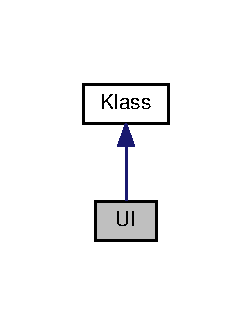
\includegraphics[width=121pt]{class_k_1_1_u_i__inherit__graph}
\end{center}
\end{figure}


Collaboration diagram for UI\+:
\nopagebreak
\begin{figure}[H]
\begin{center}
\leavevmode
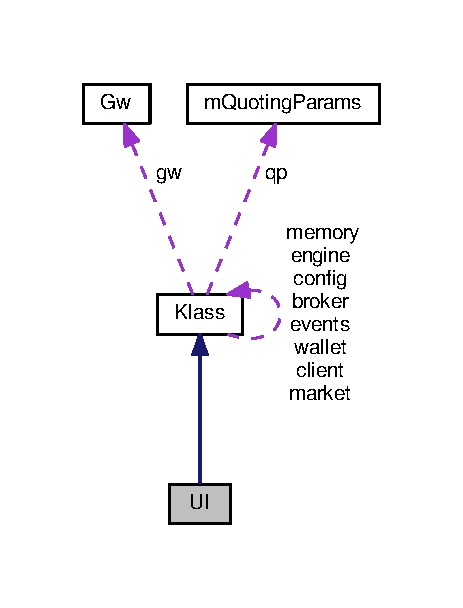
\includegraphics[width=222pt]{class_k_1_1_u_i__coll__graph}
\end{center}
\end{figure}
\subsection*{Data Fields}
\begin{DoxyCompactItemize}
\item 
unsigned int \hyperlink{class_k_1_1_u_i_a44abb2b500cfc21ada184903fb08f22d}{orders\+\_\+60s} = 0
\item 
function$<$ void(\hyperlink{namespace_k_a06e0333f0bcd3fc79835735bb9cda73d}{m\+Matter}, function$<$ void(json $\ast$)$>$ $\ast$)$>$ \hyperlink{class_k_1_1_u_i_aee907877a47fa78974d6b9a2ed1d1fad}{welcome}
\item 
function$<$ void(\hyperlink{namespace_k_a06e0333f0bcd3fc79835735bb9cda73d}{m\+Matter}, function$<$ void(json)$>$ $\ast$)$>$ \hyperlink{class_k_1_1_u_i_ad892fbcdba0fed791f3afcf1bdd0e8c7}{clickme}
\item 
function$<$ void(unsigned int)$>$ \hyperlink{class_k_1_1_u_i_aa83b4957f3c3b6166c641811adc7ebff}{delayme}
\item 
function$<$ void(\hyperlink{namespace_k_a06e0333f0bcd3fc79835735bb9cda73d}{m\+Matter}, json)$>$ \hyperlink{class_k_1_1_u_i_ac38fb07fa9906993bdfa70f5005037c2}{send}
\end{DoxyCompactItemize}
\subsection*{Protected Member Functions}
\begin{DoxyCompactItemize}
\item 
void \hyperlink{class_k_1_1_u_i_a78f61ac2dd03bcba8e09ca20cd7d68e3}{load} ()
\item 
void \hyperlink{class_k_1_1_u_i_aa9a0f090ee360e2a9f967200d30f4a22}{wait\+Data} ()
\item 
void \hyperlink{class_k_1_1_u_i_ade4c89163dbda531e71c8c75eb2868b4}{wait\+Time} ()
\item 
void \hyperlink{class_k_1_1_u_i_aa3f7b56799f5915cfbc902f6426c2bb2}{wait\+User} ()
\item 
void \hyperlink{class_k_1_1_u_i_a13a43e6d814de94978c515cb084873b1}{run} ()
\end{DoxyCompactItemize}
\subsection*{Additional Inherited Members}


\subsection{Detailed Description}


Definition at line 11 of file ui.\+h.



\subsection{Member Function Documentation}
\index{K\+::\+UI@{K\+::\+UI}!load@{load}}
\index{load@{load}!K\+::\+UI@{K\+::\+UI}}
\subsubsection[{\texorpdfstring{load()}{load()}}]{\setlength{\rightskip}{0pt plus 5cm}void load (
\begin{DoxyParamCaption}
{}
\end{DoxyParamCaption}
)\hspace{0.3cm}{\ttfamily [inline]}, {\ttfamily [protected]}, {\ttfamily [virtual]}}\hypertarget{class_k_1_1_u_i_a78f61ac2dd03bcba8e09ca20cd7d68e3}{}\label{class_k_1_1_u_i_a78f61ac2dd03bcba8e09ca20cd7d68e3}


Reimplemented from \hyperlink{class_k_1_1_klass_a5588964fff1d1025245d134e159b60ee}{Klass}.



Definition at line 25 of file ui.\+h.

\index{K\+::\+UI@{K\+::\+UI}!run@{run}}
\index{run@{run}!K\+::\+UI@{K\+::\+UI}}
\subsubsection[{\texorpdfstring{run()}{run()}}]{\setlength{\rightskip}{0pt plus 5cm}void run (
\begin{DoxyParamCaption}
{}
\end{DoxyParamCaption}
)\hspace{0.3cm}{\ttfamily [inline]}, {\ttfamily [protected]}, {\ttfamily [virtual]}}\hypertarget{class_k_1_1_u_i_a13a43e6d814de94978c515cb084873b1}{}\label{class_k_1_1_u_i_a13a43e6d814de94978c515cb084873b1}


Reimplemented from \hyperlink{class_k_1_1_klass_a72fcb26a14f6beb1c3fbace9ab3e7dbb}{Klass}.



Definition at line 144 of file ui.\+h.

\index{K\+::\+UI@{K\+::\+UI}!wait\+Data@{wait\+Data}}
\index{wait\+Data@{wait\+Data}!K\+::\+UI@{K\+::\+UI}}
\subsubsection[{\texorpdfstring{wait\+Data()}{waitData()}}]{\setlength{\rightskip}{0pt plus 5cm}void wait\+Data (
\begin{DoxyParamCaption}
{}
\end{DoxyParamCaption}
)\hspace{0.3cm}{\ttfamily [inline]}, {\ttfamily [protected]}, {\ttfamily [virtual]}}\hypertarget{class_k_1_1_u_i_aa9a0f090ee360e2a9f967200d30f4a22}{}\label{class_k_1_1_u_i_aa9a0f090ee360e2a9f967200d30f4a22}


Reimplemented from \hyperlink{class_k_1_1_klass_a62a6bf36d7c8bec9dcf7af20c9d21d74}{Klass}.



Definition at line 32 of file ui.\+h.

\index{K\+::\+UI@{K\+::\+UI}!wait\+Time@{wait\+Time}}
\index{wait\+Time@{wait\+Time}!K\+::\+UI@{K\+::\+UI}}
\subsubsection[{\texorpdfstring{wait\+Time()}{waitTime()}}]{\setlength{\rightskip}{0pt plus 5cm}void wait\+Time (
\begin{DoxyParamCaption}
{}
\end{DoxyParamCaption}
)\hspace{0.3cm}{\ttfamily [inline]}, {\ttfamily [protected]}, {\ttfamily [virtual]}}\hypertarget{class_k_1_1_u_i_ade4c89163dbda531e71c8c75eb2868b4}{}\label{class_k_1_1_u_i_ade4c89163dbda531e71c8c75eb2868b4}


Reimplemented from \hyperlink{class_k_1_1_klass_a60afdc2eaa268d8c41a2d6897fbf4fff}{Klass}.



Definition at line 124 of file ui.\+h.

\index{K\+::\+UI@{K\+::\+UI}!wait\+User@{wait\+User}}
\index{wait\+User@{wait\+User}!K\+::\+UI@{K\+::\+UI}}
\subsubsection[{\texorpdfstring{wait\+User()}{waitUser()}}]{\setlength{\rightskip}{0pt plus 5cm}void wait\+User (
\begin{DoxyParamCaption}
{}
\end{DoxyParamCaption}
)\hspace{0.3cm}{\ttfamily [inline]}, {\ttfamily [protected]}, {\ttfamily [virtual]}}\hypertarget{class_k_1_1_u_i_aa3f7b56799f5915cfbc902f6426c2bb2}{}\label{class_k_1_1_u_i_aa3f7b56799f5915cfbc902f6426c2bb2}


Reimplemented from \hyperlink{class_k_1_1_klass_af4f5201bed25a292d8a7f40470d83923}{Klass}.



Definition at line 129 of file ui.\+h.



\subsection{Field Documentation}
\index{K\+::\+UI@{K\+::\+UI}!clickme@{clickme}}
\index{clickme@{clickme}!K\+::\+UI@{K\+::\+UI}}
\subsubsection[{\texorpdfstring{clickme}{clickme}}]{\setlength{\rightskip}{0pt plus 5cm}function$<$void({\bf m\+Matter}, function$<$void(json)$>$$\ast$)$>$ clickme}\hypertarget{class_k_1_1_u_i_ad892fbcdba0fed791f3afcf1bdd0e8c7}{}\label{class_k_1_1_u_i_ad892fbcdba0fed791f3afcf1bdd0e8c7}
{\bfseries Initial value\+:}
\begin{DoxyCode}
= [&](\hyperlink{namespace_k_a06e0333f0bcd3fc79835735bb9cda73d}{mMatter} type, function<void(json)> *fn) \{
        \textcolor{keywordflow}{if} (kisses.find((\textcolor{keywordtype}{char})type) != kisses.end())
          exit(\hyperlink{sh_8h_a7a276367773516f9f6e660c3f4635beb}{\_redAlert\_}(\textcolor{stringliteral}{"UI"}, \textcolor{keywordtype}{string}(\textcolor{stringliteral}{"Use only a single unique message handler for \(\backslash\)""})
            + (\textcolor{keywordtype}{char})type + \textcolor{stringliteral}{"\(\backslash\)" clickme event"}));
        kisses[(char)type] = fn;
      \}
\end{DoxyCode}


Definition at line 155 of file ui.\+h.

\index{K\+::\+UI@{K\+::\+UI}!delayme@{delayme}}
\index{delayme@{delayme}!K\+::\+UI@{K\+::\+UI}}
\subsubsection[{\texorpdfstring{delayme}{delayme}}]{\setlength{\rightskip}{0pt plus 5cm}function$<$void(unsigned int)$>$ delayme}\hypertarget{class_k_1_1_u_i_aa83b4957f3c3b6166c641811adc7ebff}{}\label{class_k_1_1_u_i_aa83b4957f3c3b6166c641811adc7ebff}
{\bfseries Initial value\+:}
\begin{DoxyCode}
= [&](\textcolor{keywordtype}{unsigned} \textcolor{keywordtype}{int} delayUI) \{
        realtimeClient = !delayUI;
        ((EV*)\hyperlink{class_k_1_1_klass_aef02c650240e6291d8a616cda222d890}{events})->tClient->stop();
        ((EV*)\hyperlink{class_k_1_1_klass_aef02c650240e6291d8a616cda222d890}{events})->tClient->start(timer, 0, realtimeClient ? 6e+4 : delayUI * 1e+3);
      \}
\end{DoxyCode}


Definition at line 161 of file ui.\+h.

\index{K\+::\+UI@{K\+::\+UI}!orders\+\_\+60s@{orders\+\_\+60s}}
\index{orders\+\_\+60s@{orders\+\_\+60s}!K\+::\+UI@{K\+::\+UI}}
\subsubsection[{\texorpdfstring{orders\+\_\+60s}{orders_60s}}]{\setlength{\rightskip}{0pt plus 5cm}unsigned int orders\+\_\+60s = 0}\hypertarget{class_k_1_1_u_i_a44abb2b500cfc21ada184903fb08f22d}{}\label{class_k_1_1_u_i_a44abb2b500cfc21ada184903fb08f22d}


Definition at line 23 of file ui.\+h.

\index{K\+::\+UI@{K\+::\+UI}!send@{send}}
\index{send@{send}!K\+::\+UI@{K\+::\+UI}}
\subsubsection[{\texorpdfstring{send}{send}}]{\setlength{\rightskip}{0pt plus 5cm}function$<$void({\bf m\+Matter}, json)$>$ send}\hypertarget{class_k_1_1_u_i_ac38fb07fa9906993bdfa70f5005037c2}{}\label{class_k_1_1_u_i_ac38fb07fa9906993bdfa70f5005037c2}
{\bfseries Initial value\+:}
\begin{DoxyCode}
= [&](\hyperlink{namespace_k_a06e0333f0bcd3fc79835735bb9cda73d}{mMatter} type, json msg) \{
        \textcolor{keywordflow}{if} (connections == 0) \textcolor{keywordflow}{return};
        \textcolor{keywordtype}{bool} delayed = (
          type == \hyperlink{namespace_k_a06e0333f0bcd3fc79835735bb9cda73da95c17992a2bcf98203f6a1048774b1f7}{mMatter::FairValue}
          or type == \hyperlink{namespace_k_a06e0333f0bcd3fc79835735bb9cda73daef06507b3899c1e8b810bb8cbeba2b76}{mMatter::OrderStatusReports}
          or type == \hyperlink{namespace_k_a06e0333f0bcd3fc79835735bb9cda73da87c2649b2d5af994788d90af72bc3a9c}{mMatter::QuoteStatus}
          or type == \hyperlink{namespace_k_a06e0333f0bcd3fc79835735bb9cda73da52f5e0bc3859bc5f5e25130b6c7e8881}{mMatter::Position}
          or type == \hyperlink{namespace_k_a06e0333f0bcd3fc79835735bb9cda73dabe5c6be5c4decaf0b568f57bde929b6e}{mMatter::TargetBasePosition}
          or type == \hyperlink{namespace_k_a06e0333f0bcd3fc79835735bb9cda73dac68b9ff55f400f5dd9adcd7a3f5372e4}{mMatter::EWMAChart}
        );
        \textcolor{keywordflow}{if} (realtimeClient or !delayed)
          broadcast(type, msg.dump());
        \textcolor{keywordflow}{else} queue[type] = msg.dump();
      \}
\end{DoxyCode}


Definition at line 166 of file ui.\+h.

\index{K\+::\+UI@{K\+::\+UI}!welcome@{welcome}}
\index{welcome@{welcome}!K\+::\+UI@{K\+::\+UI}}
\subsubsection[{\texorpdfstring{welcome}{welcome}}]{\setlength{\rightskip}{0pt plus 5cm}function$<$void({\bf m\+Matter}, function$<$void(json$\ast$)$>$$\ast$)$>$ welcome}\hypertarget{class_k_1_1_u_i_aee907877a47fa78974d6b9a2ed1d1fad}{}\label{class_k_1_1_u_i_aee907877a47fa78974d6b9a2ed1d1fad}
{\bfseries Initial value\+:}
\begin{DoxyCode}
= [&](\hyperlink{namespace_k_a06e0333f0bcd3fc79835735bb9cda73d}{mMatter} type, function<void(json*)> *fn) \{
        \textcolor{keywordflow}{if} (hello.find((\textcolor{keywordtype}{char})type) != hello.end())
          exit(\hyperlink{sh_8h_a7a276367773516f9f6e660c3f4635beb}{\_redAlert\_}(\textcolor{stringliteral}{"UI"}, \textcolor{keywordtype}{string}(\textcolor{stringliteral}{"Use only a single unique message handler for \(\backslash\)""})
            + (\textcolor{keywordtype}{char})type + \textcolor{stringliteral}{"\(\backslash\)" welcome event"}));
        hello[(char)type] = fn;
      \}
\end{DoxyCode}


Definition at line 149 of file ui.\+h.



The documentation for this class was generated from the following file\+:\begin{DoxyCompactItemize}
\item 
\hyperlink{ui_8h}{ui.\+h}\end{DoxyCompactItemize}

\chapter{File Documentation}
\hypertarget{cf_8h}{}\section{cf.\+h File Reference}
\label{cf_8h}\index{cf.\+h@{cf.\+h}}
This graph shows which files directly or indirectly include this file\+:
\nopagebreak
\begin{figure}[H]
\begin{center}
\leavevmode
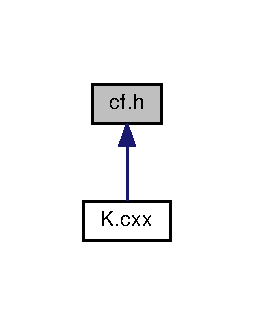
\includegraphics[width=122pt]{cf_8h__dep__incl}
\end{center}
\end{figure}
\subsection*{Data Structures}
\begin{DoxyCompactItemize}
\item 
class \hyperlink{class_k_1_1_c_f}{CF}
\end{DoxyCompactItemize}
\subsection*{Namespaces}
\begin{DoxyCompactItemize}
\item 
 \hyperlink{namespace_k}{K}
\end{DoxyCompactItemize}

\hypertarget{db_8h}{}\section{db.\+h File Reference}
\label{db_8h}\index{db.\+h@{db.\+h}}
This graph shows which files directly or indirectly include this file\+:
\nopagebreak
\begin{figure}[H]
\begin{center}
\leavevmode
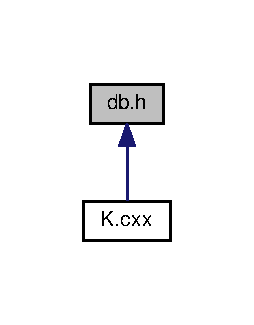
\includegraphics[width=122pt]{db_8h__dep__incl}
\end{center}
\end{figure}
\subsection*{Data Structures}
\begin{DoxyCompactItemize}
\item 
class \hyperlink{class_k_1_1_d_b}{DB}
\end{DoxyCompactItemize}
\subsection*{Namespaces}
\begin{DoxyCompactItemize}
\item 
 \hyperlink{namespace_k}{K}
\end{DoxyCompactItemize}
\subsection*{Macros}
\begin{DoxyCompactItemize}
\item 
\#define \hyperlink{db_8h_acf5e9e10b7bd5d201dcb8b6c20c45e25}{\+\_\+table\+\_\+}(k)~(k == m\+Matter\+::\+Quoting\+Parameters ? qpdb \+: \char`\"{}main\char`\"{}) + \char`\"{}.\char`\"{} + (char)k
\end{DoxyCompactItemize}


\subsection{Macro Definition Documentation}
\index{db.\+h@{db.\+h}!\+\_\+table\+\_\+@{\+\_\+table\+\_\+}}
\index{\+\_\+table\+\_\+@{\+\_\+table\+\_\+}!db.\+h@{db.\+h}}
\subsubsection[{\texorpdfstring{\+\_\+table\+\_\+}{_table_}}]{\setlength{\rightskip}{0pt plus 5cm}\#define \+\_\+table\+\_\+(
\begin{DoxyParamCaption}
\item[{}]{k}
\end{DoxyParamCaption}
)~(k == m\+Matter\+::\+Quoting\+Parameters ? qpdb \+: \char`\"{}main\char`\"{}) + \char`\"{}.\char`\"{} + (char)k}\hypertarget{db_8h_acf5e9e10b7bd5d201dcb8b6c20c45e25}{}\label{db_8h_acf5e9e10b7bd5d201dcb8b6c20c45e25}


Definition at line 4 of file db.\+h.


\hypertarget{ev_8h}{}\section{ev.\+h File Reference}
\label{ev_8h}\index{ev.\+h@{ev.\+h}}
This graph shows which files directly or indirectly include this file\+:
\nopagebreak
\begin{figure}[H]
\begin{center}
\leavevmode
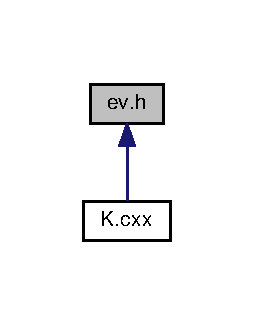
\includegraphics[width=122pt]{ev_8h__dep__incl}
\end{center}
\end{figure}
\subsection*{Data Structures}
\begin{DoxyCompactItemize}
\item 
class \hyperlink{class_k_1_1_e_v}{EV}
\end{DoxyCompactItemize}
\subsection*{Namespaces}
\begin{DoxyCompactItemize}
\item 
 \hyperlink{namespace_k}{K}
\end{DoxyCompactItemize}
\subsection*{Macros}
\begin{DoxyCompactItemize}
\item 
\#define \hyperlink{ev_8h_ab96dcc845e16d51b3adbdb0cc9f39be1}{\+\_\+debug\+Event\+\_\+}~((EV$\ast$)events)-\/$>$debug(\+\_\+\+\_\+\+P\+R\+E\+T\+T\+Y\+\_\+\+F\+U\+N\+C\+T\+I\+O\+N\+\_\+\+\_\+);
\end{DoxyCompactItemize}
\subsection*{Variables}
\begin{DoxyCompactItemize}
\item 
string \hyperlink{namespace_k_a8cf9916382d8c2046656233c4422022d}{tracelog}
\end{DoxyCompactItemize}


\subsection{Macro Definition Documentation}
\index{ev.\+h@{ev.\+h}!\+\_\+debug\+Event\+\_\+@{\+\_\+debug\+Event\+\_\+}}
\index{\+\_\+debug\+Event\+\_\+@{\+\_\+debug\+Event\+\_\+}!ev.\+h@{ev.\+h}}
\subsubsection[{\texorpdfstring{\+\_\+debug\+Event\+\_\+}{_debugEvent_}}]{\setlength{\rightskip}{0pt plus 5cm}\#define \+\_\+debug\+Event\+\_\+~((EV$\ast$)events)-\/$>$debug(\+\_\+\+\_\+\+P\+R\+E\+T\+T\+Y\+\_\+\+F\+U\+N\+C\+T\+I\+O\+N\+\_\+\+\_\+);}\hypertarget{ev_8h_ab96dcc845e16d51b3adbdb0cc9f39be1}{}\label{ev_8h_ab96dcc845e16d51b3adbdb0cc9f39be1}


Definition at line 4 of file ev.\+h.


\hypertarget{fn_8h}{}\section{fn.\+h File Reference}
\label{fn_8h}\index{fn.\+h@{fn.\+h}}
This graph shows which files directly or indirectly include this file\+:
\nopagebreak
\begin{figure}[H]
\begin{center}
\leavevmode
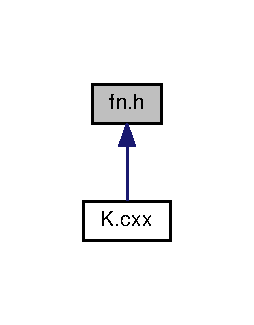
\includegraphics[width=122pt]{fn_8h__dep__incl}
\end{center}
\end{figure}
\subsection*{Data Structures}
\begin{DoxyCompactItemize}
\item 
class \hyperlink{class_k_1_1_f_n}{FN}
\end{DoxyCompactItemize}
\subsection*{Namespaces}
\begin{DoxyCompactItemize}
\item 
 \hyperlink{namespace_k}{K}
\end{DoxyCompactItemize}
\subsection*{Macros}
\begin{DoxyCompactItemize}
\item 
\#define \hyperlink{fn_8h_a597a559dabd3d64ceb55c5f4aa236187}{\+\_\+nums\+Az\+\_\+}
\item 
\#define \hyperlink{fn_8h_a8e4989b59a9e6ba0edbf26978c7a4f38}{\+\_\+\+Tclock\+\_\+}~chrono\+::system\+\_\+clock\+::now()
\item 
\#define \hyperlink{fn_8h_af2447862212be4677b0862ae1acdc09b}{\+\_\+\+Tstamp\+\_\+}
\item 
\#define \hyperlink{fn_8h_a4b3437698886f7761ab3eede7b794220}{\+\_\+fixed\+X\+\_\+}(d,  s,  X)
\item 
\#define \hyperlink{fn_8h_a3d5a9f907b48f77b76e04ecbeb005cef}{\+\_\+fixed8\+\_\+}(d,  s)~\hyperlink{fn_8h_a4b3437698886f7761ab3eede7b794220}{\+\_\+fixed\+X\+\_\+}(d, s, 8)
\item 
\#define \hyperlink{fn_8h_a346f536e7c4d9b061b2a4d3e5ea3f550}{\+\_\+trunc8\+\_\+}(d)
\end{DoxyCompactItemize}


\subsection{Macro Definition Documentation}
\index{fn.\+h@{fn.\+h}!\+\_\+fixed8\+\_\+@{\+\_\+fixed8\+\_\+}}
\index{\+\_\+fixed8\+\_\+@{\+\_\+fixed8\+\_\+}!fn.\+h@{fn.\+h}}
\subsubsection[{\texorpdfstring{\+\_\+fixed8\+\_\+}{_fixed8_}}]{\setlength{\rightskip}{0pt plus 5cm}\#define \+\_\+fixed8\+\_\+(
\begin{DoxyParamCaption}
\item[{}]{d, }
\item[{}]{s}
\end{DoxyParamCaption}
)~{\bf \+\_\+fixed\+X\+\_\+}(d, s, 8)}\hypertarget{fn_8h_a3d5a9f907b48f77b76e04ecbeb005cef}{}\label{fn_8h_a3d5a9f907b48f77b76e04ecbeb005cef}


Definition at line 19 of file fn.\+h.

\index{fn.\+h@{fn.\+h}!\+\_\+fixed\+X\+\_\+@{\+\_\+fixed\+X\+\_\+}}
\index{\+\_\+fixed\+X\+\_\+@{\+\_\+fixed\+X\+\_\+}!fn.\+h@{fn.\+h}}
\subsubsection[{\texorpdfstring{\+\_\+fixed\+X\+\_\+}{_fixedX_}}]{\setlength{\rightskip}{0pt plus 5cm}\#define \+\_\+fixed\+X\+\_\+(
\begin{DoxyParamCaption}
\item[{}]{d, }
\item[{}]{s, }
\item[{}]{X}
\end{DoxyParamCaption}
)}\hypertarget{fn_8h_a4b3437698886f7761ab3eede7b794220}{}\label{fn_8h_a4b3437698886f7761ab3eede7b794220}
{\bfseries Value\+:}
\begin{DoxyCode}
\{ stringstream ss;     \(\backslash\)
                           ss << setprecision(X) \(\backslash\)
                              << fixed << d;     \(\backslash\)
                           s = ss.str();         \}
\end{DoxyCode}


Definition at line 14 of file fn.\+h.

\index{fn.\+h@{fn.\+h}!\+\_\+nums\+Az\+\_\+@{\+\_\+nums\+Az\+\_\+}}
\index{\+\_\+nums\+Az\+\_\+@{\+\_\+nums\+Az\+\_\+}!fn.\+h@{fn.\+h}}
\subsubsection[{\texorpdfstring{\+\_\+nums\+Az\+\_\+}{_numsAz_}}]{\setlength{\rightskip}{0pt plus 5cm}\#define \+\_\+nums\+Az\+\_\+}\hypertarget{fn_8h_a597a559dabd3d64ceb55c5f4aa236187}{}\label{fn_8h_a597a559dabd3d64ceb55c5f4aa236187}
{\bfseries Value\+:}
\begin{DoxyCode}
\textcolor{stringliteral}{"0123456789"}                 \(\backslash\)
                 \textcolor{stringliteral}{"ABCDEFGHIJKLMNOPQRSTUVWXYZ"} \(\backslash\)
                 \textcolor{stringliteral}{"abcdefghijklmnopqrstuvwxyz"}
\end{DoxyCode}


Definition at line 4 of file fn.\+h.

\index{fn.\+h@{fn.\+h}!\+\_\+\+Tclock\+\_\+@{\+\_\+\+Tclock\+\_\+}}
\index{\+\_\+\+Tclock\+\_\+@{\+\_\+\+Tclock\+\_\+}!fn.\+h@{fn.\+h}}
\subsubsection[{\texorpdfstring{\+\_\+\+Tclock\+\_\+}{_Tclock_}}]{\setlength{\rightskip}{0pt plus 5cm}\#define \+\_\+\+Tclock\+\_\+~chrono\+::system\+\_\+clock\+::now()}\hypertarget{fn_8h_a8e4989b59a9e6ba0edbf26978c7a4f38}{}\label{fn_8h_a8e4989b59a9e6ba0edbf26978c7a4f38}


Definition at line 8 of file fn.\+h.

\index{fn.\+h@{fn.\+h}!\+\_\+trunc8\+\_\+@{\+\_\+trunc8\+\_\+}}
\index{\+\_\+trunc8\+\_\+@{\+\_\+trunc8\+\_\+}!fn.\+h@{fn.\+h}}
\subsubsection[{\texorpdfstring{\+\_\+trunc8\+\_\+}{_trunc8_}}]{\setlength{\rightskip}{0pt plus 5cm}\#define \+\_\+trunc8\+\_\+(
\begin{DoxyParamCaption}
\item[{}]{d}
\end{DoxyParamCaption}
)}\hypertarget{fn_8h_a346f536e7c4d9b061b2a4d3e5ea3f550}{}\label{fn_8h_a346f536e7c4d9b061b2a4d3e5ea3f550}
{\bfseries Value\+:}
\begin{DoxyCode}
\{ \textcolor{keywordtype}{string} s;      \hyperlink{fn_8h_a3d5a9f907b48f77b76e04ecbeb005cef}{\(\backslash\)}
\hyperlink{fn_8h_a3d5a9f907b48f77b76e04ecbeb005cef}{                      \_fixed8\_}(d, s) \(\backslash\)
                      d = stod(s);   \}
\end{DoxyCode}


Definition at line 21 of file fn.\+h.

\index{fn.\+h@{fn.\+h}!\+\_\+\+Tstamp\+\_\+@{\+\_\+\+Tstamp\+\_\+}}
\index{\+\_\+\+Tstamp\+\_\+@{\+\_\+\+Tstamp\+\_\+}!fn.\+h@{fn.\+h}}
\subsubsection[{\texorpdfstring{\+\_\+\+Tstamp\+\_\+}{_Tstamp_}}]{\setlength{\rightskip}{0pt plus 5cm}\#define \+\_\+\+Tstamp\+\_\+}\hypertarget{fn_8h_af2447862212be4677b0862ae1acdc09b}{}\label{fn_8h_af2447862212be4677b0862ae1acdc09b}
{\bfseries Value\+:}
\begin{DoxyCode}
chrono::duration\_cast<chrono::milliseconds>( \hyperlink{fn_8h_a8e4989b59a9e6ba0edbf26978c7a4f38}{\(\backslash\)}
\hyperlink{fn_8h_a8e4989b59a9e6ba0edbf26978c7a4f38}{                   \_Tclock\_}.time\_since\_epoch()                \(\backslash\)
                 ).count()
\end{DoxyCode}


Definition at line 10 of file fn.\+h.


\hypertarget{gw_8h}{}\section{gw.\+h File Reference}
\label{gw_8h}\index{gw.\+h@{gw.\+h}}
This graph shows which files directly or indirectly include this file\+:
\nopagebreak
\begin{figure}[H]
\begin{center}
\leavevmode
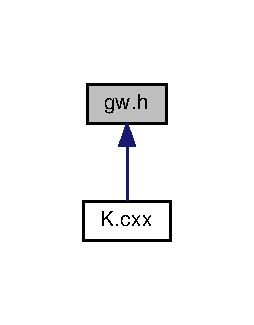
\includegraphics[width=122pt]{gw_8h__dep__incl}
\end{center}
\end{figure}
\subsection*{Data Structures}
\begin{DoxyCompactItemize}
\item 
class \hyperlink{class_k_1_1_g_w}{GW}
\end{DoxyCompactItemize}
\subsection*{Namespaces}
\begin{DoxyCompactItemize}
\item 
 \hyperlink{namespace_k}{K}
\end{DoxyCompactItemize}

\hypertarget{_k_8cxx}{}\section{K.\+cxx File Reference}
\label{_k_8cxx}\index{K.\+cxx@{K.\+cxx}}
{\ttfamily \#include $<$stdlib.\+h$>$}\\*
{\ttfamily \#include $<$iostream$>$}\\*
{\ttfamily \#include $<$sstream$>$}\\*
{\ttfamily \#include $<$string$>$}\\*
{\ttfamily \#include $<$random$>$}\\*
{\ttfamily \#include $<$thread$>$}\\*
{\ttfamily \#include $<$mutex$>$}\\*
{\ttfamily \#include $<$future$>$}\\*
{\ttfamily \#include $<$chrono$>$}\\*
{\ttfamily \#include $<$locale$>$}\\*
{\ttfamily \#include $<$time.\+h$>$}\\*
{\ttfamily \#include $<$math.\+h$>$}\\*
{\ttfamily \#include $<$getopt.\+h$>$}\\*
{\ttfamily \#include $<$signal.\+h$>$}\\*
{\ttfamily \#include $<$functional$>$}\\*
{\ttfamily \#include $<$algorithm$>$}\\*
{\ttfamily \#include $<$iomanip$>$}\\*
{\ttfamily \#include $<$vector$>$}\\*
{\ttfamily \#include $<$map$>$}\\*
{\ttfamily \#include $<$execinfo.\+h$>$}\\*
{\ttfamily \#include \char`\"{}json.\+h\char`\"{}}\\*
{\ttfamily \#include \char`\"{}sqlite3.\+h\char`\"{}}\\*
{\ttfamily \#include \char`\"{}u\+W\+S/u\+W\+S.\+h\char`\"{}}\\*
{\ttfamily \#include \char`\"{}curl/curl.\+h\char`\"{}}\\*
{\ttfamily \#include \char`\"{}openssl/md5.\+h\char`\"{}}\\*
{\ttfamily \#include \char`\"{}openssl/bio.\+h\char`\"{}}\\*
{\ttfamily \#include \char`\"{}openssl/evp.\+h\char`\"{}}\\*
{\ttfamily \#include \char`\"{}openssl/sha.\+h\char`\"{}}\\*
{\ttfamily \#include \char`\"{}openssl/hmac.\+h\char`\"{}}\\*
{\ttfamily \#include \char`\"{}openssl/buffer.\+h\char`\"{}}\\*
{\ttfamily \#include \char`\"{}ncurses/ncurses.\+h\char`\"{}}\\*
{\ttfamily \#include \char`\"{}quickfix/\+Null\+Store.\+h\char`\"{}}\\*
{\ttfamily \#include \char`\"{}quickfix/\+Application.\+h\char`\"{}}\\*
{\ttfamily \#include \char`\"{}quickfix/\+Socket\+Initiator.\+h\char`\"{}}\\*
{\ttfamily \#include \char`\"{}quickfix/\+Session\+Settings.\+h\char`\"{}}\\*
{\ttfamily \#include \char`\"{}quickfix/fix42/\+New\+Order\+Single.\+h\char`\"{}}\\*
{\ttfamily \#include \char`\"{}quickfix/fix42/\+Order\+Cancel\+Request.\+h\char`\"{}}\\*
{\ttfamily \#include \char`\"{}fn.\+h\char`\"{}}\\*
{\ttfamily \#include \char`\"{}km.\+h\char`\"{}}\\*
{\ttfamily \#include \char`\"{}sh.\+h\char`\"{}}\\*
{\ttfamily \#include \char`\"{}cf.\+h\char`\"{}}\\*
{\ttfamily \#include \char`\"{}ev.\+h\char`\"{}}\\*
{\ttfamily \#include \char`\"{}db.\+h\char`\"{}}\\*
{\ttfamily \#include \char`\"{}ui.\+h\char`\"{}}\\*
{\ttfamily \#include \char`\"{}qp.\+h\char`\"{}}\\*
{\ttfamily \#include \char`\"{}og.\+h\char`\"{}}\\*
{\ttfamily \#include \char`\"{}mg.\+h\char`\"{}}\\*
{\ttfamily \#include \char`\"{}pg.\+h\char`\"{}}\\*
{\ttfamily \#include \char`\"{}qe.\+h\char`\"{}}\\*
{\ttfamily \#include \char`\"{}gw.\+h\char`\"{}}\\*
\subsection*{Functions}
\begin{DoxyCompactItemize}
\item 
int \hyperlink{_k_8cxx_a3c04138a5bfe5d72780bb7e82a18e627}{main} (int argc, char $\ast$$\ast$argv)
\end{DoxyCompactItemize}


\subsection{Function Documentation}
\index{K.\+cxx@{K.\+cxx}!main@{main}}
\index{main@{main}!K.\+cxx@{K.\+cxx}}
\subsubsection[{\texorpdfstring{main(int argc, char $\ast$$\ast$argv)}{main(int argc, char **argv)}}]{\setlength{\rightskip}{0pt plus 5cm}int main (
\begin{DoxyParamCaption}
\item[{int}]{argc, }
\item[{char $\ast$$\ast$}]{argv}
\end{DoxyParamCaption}
)}\hypertarget{_k_8cxx_a3c04138a5bfe5d72780bb7e82a18e627}{}\label{_k_8cxx_a3c04138a5bfe5d72780bb7e82a18e627}


Definition at line 62 of file K.\+cxx.


\hypertarget{km_8h}{}\section{km.\+h File Reference}
\label{km_8h}\index{km.\+h@{km.\+h}}
This graph shows which files directly or indirectly include this file\+:
\nopagebreak
\begin{figure}[H]
\begin{center}
\leavevmode
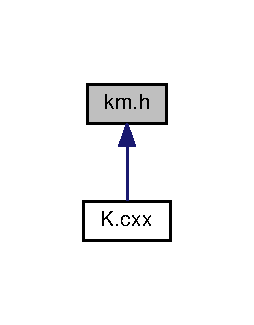
\includegraphics[width=122pt]{km_8h__dep__incl}
\end{center}
\end{figure}
\subsection*{Data Structures}
\begin{DoxyCompactItemize}
\item 
struct \hyperlink{struct_k_1_1m_quoting_params}{m\+Quoting\+Params}
\item 
struct \hyperlink{struct_k_1_1m_pair}{m\+Pair}
\item 
struct \hyperlink{struct_k_1_1m_wallet}{m\+Wallet}
\item 
struct \hyperlink{struct_k_1_1m_wallets}{m\+Wallets}
\item 
struct \hyperlink{struct_k_1_1m_profit}{m\+Profit}
\item 
struct \hyperlink{struct_k_1_1m_safety}{m\+Safety}
\item 
struct \hyperlink{struct_k_1_1m_position}{m\+Position}
\item 
struct \hyperlink{struct_k_1_1m_trade}{m\+Trade}
\item 
struct \hyperlink{struct_k_1_1m_order}{m\+Order}
\item 
struct \hyperlink{struct_k_1_1m_level}{m\+Level}
\item 
struct \hyperlink{struct_k_1_1m_levels}{m\+Levels}
\item 
struct \hyperlink{struct_k_1_1m_levels_diff}{m\+Levels\+Diff}
\item 
struct \hyperlink{struct_k_1_1m_quote}{m\+Quote}
\item 
struct \hyperlink{struct_k_1_1m_quote_status}{m\+Quote\+Status}
\item 
class \hyperlink{class_k_1_1_gw}{Gw}
\item 
class \hyperlink{class_k_1_1_klass}{Klass}
\item 
class \hyperlink{class_k_1_1k_lass}{k\+Lass}
\end{DoxyCompactItemize}
\subsection*{Namespaces}
\begin{DoxyCompactItemize}
\item 
 \hyperlink{namespace_k}{K}
\end{DoxyCompactItemize}
\subsection*{Macros}
\begin{DoxyCompactItemize}
\item 
\#define \hyperlink{km_8h_ad02a70cba4c52ba2013e5e32ceaeac1c}{m\+Clock}~unsigned long long
\item 
\#define \hyperlink{km_8h_a392f9b7f384aa3539bbb890b059f5b8c}{m\+Price}~double
\item 
\#define \hyperlink{km_8h_ad4d00888c55a47a8a40ed8020d176086}{m\+Amount}~double
\item 
\#define \hyperlink{km_8h_a23233b27e494114073abc4d494b05626}{m\+Rand\+Id}~string
\item 
\#define \hyperlink{km_8h_a0299927fb26276a1e0f4c2b4dedb698e}{m\+Coin\+Id}~string
\end{DoxyCompactItemize}
\subsection*{Enumerations}
\begin{DoxyCompactItemize}
\item 
enum \hyperlink{namespace_k_a7ab53d1849aa2c29d90459c21afa8c17}{m\+Exchange} \+: unsigned int \{ \\*
\hyperlink{namespace_k_a7ab53d1849aa2c29d90459c21afa8c17abbb93ef26e3c101ff11cdd21cab08a94}{Null}, 
\hyperlink{namespace_k_a7ab53d1849aa2c29d90459c21afa8c17ae05277537bf941fa13c912696bf55c2f}{Hit\+Btc}, 
\hyperlink{namespace_k_a7ab53d1849aa2c29d90459c21afa8c17a6af33051ce1839b748ad2f59cb203e0f}{Ok\+Coin}, 
\hyperlink{namespace_k_a7ab53d1849aa2c29d90459c21afa8c17a28d13ddddf18afba2c3727253ba0d42f}{Coinbase}, 
\\*
\hyperlink{namespace_k_a7ab53d1849aa2c29d90459c21afa8c17a4e7d470f48dde438b7e7ee118231262d}{Bitfinex}, 
\hyperlink{namespace_k_a7ab53d1849aa2c29d90459c21afa8c17a049a956dfeb0eb2e19c417a1dde4d680}{Kraken}, 
\hyperlink{namespace_k_a7ab53d1849aa2c29d90459c21afa8c17a1299d85e255e3e8967042390b25dffd3}{Ok\+Ex}, 
\hyperlink{namespace_k_a7ab53d1849aa2c29d90459c21afa8c17ac17831afdb4609a6f28e6f361c67b55f}{Bitfinex\+Margin}, 
\\*
\hyperlink{namespace_k_a7ab53d1849aa2c29d90459c21afa8c17a58fbcde0e62c0d61a359ac2cab9418c6}{Korbit}, 
\hyperlink{namespace_k_a7ab53d1849aa2c29d90459c21afa8c17a90239374e2208c9b3ad9d6ead6d875b8}{Poloniex}
 \}
\item 
enum \hyperlink{namespace_k_a3da250819294c55d5728586148bfa19e}{m\+Connectivity} \+: unsigned int \{ \hyperlink{namespace_k_a3da250819294c55d5728586148bfa19eaef70e46fd3bbc21e3e1f0b6815e750c0}{Disconnected}, 
\hyperlink{namespace_k_a3da250819294c55d5728586148bfa19ea2ec0d16e4ca169baedb9b2d50ec5c6d7}{Connected}
 \}
\item 
enum \hyperlink{namespace_k_a9ca92b450f3b1738c485770d136ac9e0}{m\+Status} \+: unsigned int \{ \hyperlink{namespace_k_a9ca92b450f3b1738c485770d136ac9e0a03c2e7e41ffc181a4e84080b4710e81e}{New}, 
\hyperlink{namespace_k_a9ca92b450f3b1738c485770d136ac9e0a829eadc8e29caab50cc26bc6a451a1f1}{Working}, 
\hyperlink{namespace_k_a9ca92b450f3b1738c485770d136ac9e0aae94f80b3ce82062a5dd7815daa04f9d}{Complete}, 
\hyperlink{namespace_k_a9ca92b450f3b1738c485770d136ac9e0aa149e85a44aeec9140e92733d9ed694e}{Cancelled}
 \}
\item 
enum \hyperlink{namespace_k_a0b7d0fa0ffc9f87da1d6499cbcee7e94}{m\+Side} \+: unsigned int \{ \hyperlink{namespace_k_a0b7d0fa0ffc9f87da1d6499cbcee7e94ae36ba1e187ae2b3ebcfd0a4c68367caf}{Bid}, 
\hyperlink{namespace_k_a0b7d0fa0ffc9f87da1d6499cbcee7e94aa0b271a9d8aa8e7473922164d6a1c03c}{Ask}, 
\hyperlink{namespace_k_a0b7d0fa0ffc9f87da1d6499cbcee7e94a130c5b3473c57faa76e2a1c54e26f88e}{Both}
 \}
\item 
enum \hyperlink{namespace_k_a290fccb3fc7d447fdbb93a61f6dfba44}{m\+Time\+In\+Force} \+: unsigned int \{ \hyperlink{namespace_k_a290fccb3fc7d447fdbb93a61f6dfba44a7245a636843f38ae56d5862d502a4303}{I\+OC}, 
\hyperlink{namespace_k_a290fccb3fc7d447fdbb93a61f6dfba44a9650d9d6d673551228bb1042f482459f}{F\+OK}, 
\hyperlink{namespace_k_a290fccb3fc7d447fdbb93a61f6dfba44a87b20a4d7f9fae0a5b12c2b9c680584b}{G\+TC}
 \}
\item 
enum \hyperlink{namespace_k_a131435180aff10fab1bf3da09af62b0d}{m\+Order\+Type} \+: unsigned int \{ \hyperlink{namespace_k_a131435180aff10fab1bf3da09af62b0da80d2677cf518f4d04320042f4ea6c146}{Limit}, 
\hyperlink{namespace_k_a131435180aff10fab1bf3da09af62b0da31840a66a8d6d223e5b0540138768838}{Market}
 \}
\item 
enum \hyperlink{namespace_k_a9d7dedf4873c0cda3ab0c919395b667c}{m\+Ping\+At} \+: unsigned int \{ \\*
\hyperlink{namespace_k_a9d7dedf4873c0cda3ab0c919395b667cad20455e0ed8edbd95fbbb7dff3d61503}{Both\+Sides}, 
\hyperlink{namespace_k_a9d7dedf4873c0cda3ab0c919395b667ca50d6b07d51e9c2741ce22c2ed476e018}{Bid\+Side}, 
\hyperlink{namespace_k_a9d7dedf4873c0cda3ab0c919395b667ca29381a34d014b448d3316e216610d1ce}{Ask\+Side}, 
\hyperlink{namespace_k_a9d7dedf4873c0cda3ab0c919395b667cac2f26a4dd047de7d95959ab8bdb109f4}{Depleted\+Side}, 
\\*
\hyperlink{namespace_k_a9d7dedf4873c0cda3ab0c919395b667ca4063c4f19b53c5df60ae4c05c9dd9a54}{Depleted\+Bid\+Side}, 
\hyperlink{namespace_k_a9d7dedf4873c0cda3ab0c919395b667caae428d5bdebd6c7b80f502858b11c8ba}{Depleted\+Ask\+Side}, 
\hyperlink{namespace_k_a9d7dedf4873c0cda3ab0c919395b667ca1ec3d10862ac7f958aad8b62285b08e9}{Stop\+Pings}
 \}
\item 
enum \hyperlink{namespace_k_a6bd1ffa01a02e9cf1302f02774ba013f}{m\+Pong\+At} \+: unsigned int \{ \\*
\hyperlink{namespace_k_a6bd1ffa01a02e9cf1302f02774ba013fa102eaf65c3a5f9be2898b918b50c0a09}{Short\+Ping\+Fair}, 
\hyperlink{namespace_k_a6bd1ffa01a02e9cf1302f02774ba013fae839dfe48819b12d62924214b21c41bb}{Average\+Ping\+Fair}, 
\hyperlink{namespace_k_a6bd1ffa01a02e9cf1302f02774ba013faea50308be4005a5288ab9ca9835eb264}{Long\+Ping\+Fair}, 
\hyperlink{namespace_k_a6bd1ffa01a02e9cf1302f02774ba013faf6faf434c7dc6b4c4c2c25e80910be93}{Short\+Ping\+Aggressive}, 
\\*
\hyperlink{namespace_k_a6bd1ffa01a02e9cf1302f02774ba013fa7ddcfa83b293abeb8713b2ce5b37ed67}{Average\+Ping\+Aggressive}, 
\hyperlink{namespace_k_a6bd1ffa01a02e9cf1302f02774ba013faef372043d682faaebb32c65219ae0b0d}{Long\+Ping\+Aggressive}
 \}
\item 
enum \hyperlink{namespace_k_aad47eca41d4abcf27209f4b673e7b9e9}{m\+Quoting\+Mode} \+: unsigned int \{ \\*
\hyperlink{namespace_k_aad47eca41d4abcf27209f4b673e7b9e9aa4ffdcf0dc1f31b9acaf295d75b51d00}{Top}, 
\hyperlink{namespace_k_aad47eca41d4abcf27209f4b673e7b9e9a55c6b09cbca39ef0cdb728eb112a5049}{Mid}, 
\hyperlink{namespace_k_aad47eca41d4abcf27209f4b673e7b9e9aa286d9991c6a547ae25a5f5216164b8f}{Join}, 
\hyperlink{namespace_k_aad47eca41d4abcf27209f4b673e7b9e9a56c381ec4d4882fef3875344e31366c4}{Inverse\+Join}, 
\\*
\hyperlink{namespace_k_aad47eca41d4abcf27209f4b673e7b9e9ad405435761161126203a203ceceb2bf6}{Inverse\+Top}, 
\hyperlink{namespace_k_aad47eca41d4abcf27209f4b673e7b9e9ade25a4b5bc9f51863b89a863fc98fdc3}{Hamelin\+Rat}, 
\hyperlink{namespace_k_aad47eca41d4abcf27209f4b673e7b9e9a675056ad1441b6375b2c5abd48c27ef1}{Depth}
 \}
\item 
enum \hyperlink{namespace_k_a89330b32d78089edeaa5bc6fe48d605d}{m\+Quoting\+Safety} \+: unsigned int \{ \hyperlink{namespace_k_a89330b32d78089edeaa5bc6fe48d605dad15305d7a4e34e02489c74a5ef542f36}{Off}, 
\hyperlink{namespace_k_a89330b32d78089edeaa5bc6fe48d605da99e52704462d3580db3528cad7ea9660}{Ping\+Pong}, 
\hyperlink{namespace_k_a89330b32d78089edeaa5bc6fe48d605da8c9d96b1ef82662dd41a42e8528876b6}{Boomerang}, 
\hyperlink{namespace_k_a89330b32d78089edeaa5bc6fe48d605da412070b7feb8fc0fe4859d864cf83596}{A\+K47}
 \}
\item 
enum \hyperlink{namespace_k_a76b6774ff9252e574d375a353ecf6736}{m\+Quote\+State} \+: unsigned int \{ \\*
\hyperlink{namespace_k_a76b6774ff9252e574d375a353ecf6736a955ad3298db330b5ee880c2c9e6f23a0}{Live}, 
\hyperlink{namespace_k_a76b6774ff9252e574d375a353ecf6736aef70e46fd3bbc21e3e1f0b6815e750c0}{Disconnected}, 
\hyperlink{namespace_k_a76b6774ff9252e574d375a353ecf6736a152243c591927afa2121aea8911cccd2}{Disabled\+Quotes}, 
\hyperlink{namespace_k_a76b6774ff9252e574d375a353ecf6736afe155956e8f33e5cffa82cc86a36afbd}{Missing\+Data}, 
\\*
\hyperlink{namespace_k_a76b6774ff9252e574d375a353ecf6736aa6dd615eded3f865e7f58d646d053222}{Unknown\+Held}, 
\hyperlink{namespace_k_a76b6774ff9252e574d375a353ecf6736aa082cb41967bd1a64dca9fd7127cb7cc}{T\+B\+P\+Held}, 
\hyperlink{namespace_k_a76b6774ff9252e574d375a353ecf6736a5faf2570a6605866bf01a5675538e511}{Max\+Trades\+Seconds}, 
\hyperlink{namespace_k_a76b6774ff9252e574d375a353ecf6736a9642b3e14fbadab3e7acfbd02cd8cc73}{Waiting\+Ping}, 
\\*
\hyperlink{namespace_k_a76b6774ff9252e574d375a353ecf6736ac390c66e7e7a9d6c107cc9f63d16fb77}{Depleted\+Funds}, 
\hyperlink{namespace_k_a76b6774ff9252e574d375a353ecf6736a23709652ceedf22aad4bbb6a355b83e2}{Crossed}, 
\hyperlink{namespace_k_a76b6774ff9252e574d375a353ecf6736abe667931a6504eeaed8bc383e0176c80}{Up\+Trend\+Held}, 
\hyperlink{namespace_k_a76b6774ff9252e574d375a353ecf6736a2d25ded63a54e99883cace0cc0877cd8}{Down\+Trend\+Held}
 \}
\item 
enum \hyperlink{namespace_k_ae4a47201f2511ecc8ab5b412e872b9dd}{m\+Fair\+Value\+Model} \+: unsigned int \{ \hyperlink{namespace_k_ae4a47201f2511ecc8ab5b412e872b9dda2a723053ab15920e0c2ecd25a2ede6f9}{B\+BO}, 
\hyperlink{namespace_k_ae4a47201f2511ecc8ab5b412e872b9ddab7a93074edb29bebc9b6144134fa4975}{w\+B\+BO}
 \}
\item 
enum \hyperlink{namespace_k_a8708a45c314b4d4bb9e7221009ccee8a}{m\+Auto\+Position\+Mode} \+: unsigned int \{ \hyperlink{namespace_k_a8708a45c314b4d4bb9e7221009ccee8aae1ba155a9f2e8c3be94020eef32a0301}{Manual}, 
\hyperlink{namespace_k_a8708a45c314b4d4bb9e7221009ccee8aab539e10bdc606700e99b1e0cff611765}{E\+W\+M\+A\+\_\+\+LS}, 
\hyperlink{namespace_k_a8708a45c314b4d4bb9e7221009ccee8aa7a06abe21a1d39768d5df863d1c9cfc4}{E\+W\+M\+A\+\_\+\+L\+MS}, 
\hyperlink{namespace_k_a8708a45c314b4d4bb9e7221009ccee8aaf907e979e96417055b1b3174b18689fd}{E\+W\+M\+A\+\_\+4}
 \}
\item 
enum \hyperlink{namespace_k_ac928319d6f2b7d9709cd3ca9fa6cb5a7}{m\+P\+Div\+Mode} \+: unsigned int \{ \\*
\hyperlink{namespace_k_ac928319d6f2b7d9709cd3ca9fa6cb5a7ae1ba155a9f2e8c3be94020eef32a0301}{Manual}, 
\hyperlink{namespace_k_ac928319d6f2b7d9709cd3ca9fa6cb5a7a32a843da6ea40ab3b17a3421ccdf671b}{Linear}, 
\hyperlink{namespace_k_ac928319d6f2b7d9709cd3ca9fa6cb5a7a6ca9e2d793f678aba7c1b19526592a46}{Sine}, 
\hyperlink{namespace_k_ac928319d6f2b7d9709cd3ca9fa6cb5a7a36875f2500a09ee35d0bb7eb8c0b91b0}{S\+Q\+RT}, 
\\*
\hyperlink{namespace_k_ac928319d6f2b7d9709cd3ca9fa6cb5a7abbc155fb2b111bf61c4f5ff892915e6b}{Switch}
 \}
\item 
enum \hyperlink{namespace_k_a8fb2f5e34d77eef380ac27a7737a3a25}{m\+A\+PR} \+: unsigned int \{ \hyperlink{namespace_k_a8fb2f5e34d77eef380ac27a7737a3a25ad15305d7a4e34e02489c74a5ef542f36}{Off}, 
\hyperlink{namespace_k_a8fb2f5e34d77eef380ac27a7737a3a25a6f6cb72d544962fa333e2e34ce64f719}{Size}, 
\hyperlink{namespace_k_a8fb2f5e34d77eef380ac27a7737a3a25a521e68d07542f40555e0bd6361547f8a}{Size\+Width}
 \}
\item 
enum \hyperlink{namespace_k_a2f7964509b276df1811f64989ee56ca5}{m\+S\+OP} \+: unsigned int \{ \hyperlink{namespace_k_a2f7964509b276df1811f64989ee56ca5ad15305d7a4e34e02489c74a5ef542f36}{Off}, 
\hyperlink{namespace_k_a2f7964509b276df1811f64989ee56ca5a18da2603c92b826445472937933895e5}{Trades}, 
\hyperlink{namespace_k_a2f7964509b276df1811f64989ee56ca5a6f6cb72d544962fa333e2e34ce64f719}{Size}, 
\hyperlink{namespace_k_a2f7964509b276df1811f64989ee56ca5a307b9b6d2f7f31e05110e3391dabb83e}{Trades\+Size}
 \}
\item 
enum \hyperlink{namespace_k_a648db17031757556a30a6ba51a9ce636}{m\+S\+T\+D\+EV} \+: unsigned int \{ \\*
\hyperlink{namespace_k_a648db17031757556a30a6ba51a9ce636ad15305d7a4e34e02489c74a5ef542f36}{Off}, 
\hyperlink{namespace_k_a648db17031757556a30a6ba51a9ce636aba195c1980354f4259bcb71e0ec84790}{On\+FV}, 
\hyperlink{namespace_k_a648db17031757556a30a6ba51a9ce636a2f95269c5b49e4c173f4434c77a5c44e}{On\+F\+V\+A\+P\+R\+Off}, 
\hyperlink{namespace_k_a648db17031757556a30a6ba51a9ce636a3cfe59668dcf743c426719e30e92a11f}{On\+Tops}, 
\\*
\hyperlink{namespace_k_a648db17031757556a30a6ba51a9ce636aca34048591922a10fc48621fc379aa11}{On\+Tops\+A\+P\+R\+Off}, 
\hyperlink{namespace_k_a648db17031757556a30a6ba51a9ce636ae1eab7ec616da449c7890bcd3f85bfa2}{On\+Top}, 
\hyperlink{namespace_k_a648db17031757556a30a6ba51a9ce636a173c34596b864ac314738d30f204a4ec}{On\+Top\+A\+P\+R\+Off}
 \}
\item 
enum \hyperlink{namespace_k_a211862d8b09ec46a051464b6859c1306}{m\+Hotkey} \+: int \{ \hyperlink{namespace_k_a211862d8b09ec46a051464b6859c1306a6351aefd1e5e1b62c76f8580116964be}{E\+SC} = 27, 
\hyperlink{namespace_k_a211862d8b09ec46a051464b6859c1306af09564c9ca56850d4cd6b3319e541aee}{Q} = 81, 
\hyperlink{namespace_k_a211862d8b09ec46a051464b6859c1306a7694f4a66316e53c8cdd9d9954bd611d}{q} = 113
 \}
\item 
enum \hyperlink{namespace_k_ab6a388ee7614dc94c1d933688d49b3bb}{m\+Portal} \+: unsigned char \{ \hyperlink{namespace_k_ab6a388ee7614dc94c1d933688d49b3bba8b1a9953c4611296a827abf8c47804d7}{Hello} = \textquotesingle{}=\textquotesingle{}, 
\hyperlink{namespace_k_ab6a388ee7614dc94c1d933688d49b3bbad61fad2618362cf5c2392d4880e3f4b4}{Kiss} = \textquotesingle{}-\/\textquotesingle{}
 \}
\item 
enum \hyperlink{namespace_k_a06e0333f0bcd3fc79835735bb9cda73d}{m\+Matter} \+: unsigned char \{ \\*
\hyperlink{namespace_k_a06e0333f0bcd3fc79835735bb9cda73da95c17992a2bcf98203f6a1048774b1f7}{Fair\+Value} = \textquotesingle{}a\textquotesingle{}, 
\hyperlink{namespace_k_a06e0333f0bcd3fc79835735bb9cda73dac48e929b2b1eabba2ba036884433345e}{Quote} = \textquotesingle{}b\textquotesingle{}, 
\hyperlink{namespace_k_a06e0333f0bcd3fc79835735bb9cda73daf18f5fdb8e039d60196b4065580640b7}{Active\+Subscription} = \textquotesingle{}c\textquotesingle{}, 
\hyperlink{namespace_k_a06e0333f0bcd3fc79835735bb9cda73da9bd9d0ebc081bd74f5bef4e136bb1aed}{Connectivity} = \textquotesingle{}d\textquotesingle{}, 
\\*
\hyperlink{namespace_k_a06e0333f0bcd3fc79835735bb9cda73dac2230c6e4d01b8865ebc4ad0aef9db94}{Market\+Data} = \textquotesingle{}e\textquotesingle{}, 
\hyperlink{namespace_k_a06e0333f0bcd3fc79835735bb9cda73daac974900d8b102bac26cc80ab192f8fb}{Quoting\+Parameters} = \textquotesingle{}f\textquotesingle{}, 
\hyperlink{namespace_k_a06e0333f0bcd3fc79835735bb9cda73dada6fe8bd0dd6e070b6638a40fed954e2}{Safety\+Settings} = \textquotesingle{}g\textquotesingle{}, 
\hyperlink{namespace_k_a06e0333f0bcd3fc79835735bb9cda73dadeb10517653c255364175796ace3553f}{Product} = \textquotesingle{}h\textquotesingle{}, 
\\*
\hyperlink{namespace_k_a06e0333f0bcd3fc79835735bb9cda73daef06507b3899c1e8b810bb8cbeba2b76}{Order\+Status\+Reports} = \textquotesingle{}i\textquotesingle{}, 
\hyperlink{namespace_k_a06e0333f0bcd3fc79835735bb9cda73da13728e0c13d8f5168df144b86053ba3c}{Product\+Advertisement} = \textquotesingle{}j\textquotesingle{}, 
\hyperlink{namespace_k_a06e0333f0bcd3fc79835735bb9cda73da06d51239dde617fbf765978bd622115c}{Application\+State} = \textquotesingle{}k\textquotesingle{}, 
\hyperlink{namespace_k_a06e0333f0bcd3fc79835735bb9cda73dad47922653f65611f6f38d4eef7b93e61}{Notepad} = \textquotesingle{}l\textquotesingle{}, 
\\*
\hyperlink{namespace_k_a06e0333f0bcd3fc79835735bb9cda73da24d3ff5461155ee60f97c12c3cb38622}{Toggle\+Settings} = \textquotesingle{}m\textquotesingle{}, 
\hyperlink{namespace_k_a06e0333f0bcd3fc79835735bb9cda73da52f5e0bc3859bc5f5e25130b6c7e8881}{Position} = \textquotesingle{}n\textquotesingle{}, 
\hyperlink{namespace_k_a06e0333f0bcd3fc79835735bb9cda73daaf1815bda3e84b3854a3b0d697437590}{Submit\+New\+Order} = \textquotesingle{}p\textquotesingle{}, 
\hyperlink{namespace_k_a06e0333f0bcd3fc79835735bb9cda73da80d0877777fae74f6486c79734cb4643}{Cancel\+Order} = \textquotesingle{}q\textquotesingle{}, 
\\*
\hyperlink{namespace_k_a06e0333f0bcd3fc79835735bb9cda73da3aac00a7768e3c27223f6bebe8675380}{Market\+Trade} = \textquotesingle{}r\textquotesingle{}, 
\hyperlink{namespace_k_a06e0333f0bcd3fc79835735bb9cda73da18da2603c92b826445472937933895e5}{Trades} = \textquotesingle{}s\textquotesingle{}, 
\hyperlink{namespace_k_a06e0333f0bcd3fc79835735bb9cda73daa47103a2cc61c37ef564115155eb5a1b}{External\+Valuation} = \textquotesingle{}t\textquotesingle{}, 
\hyperlink{namespace_k_a06e0333f0bcd3fc79835735bb9cda73da87c2649b2d5af994788d90af72bc3a9c}{Quote\+Status} = \textquotesingle{}u\textquotesingle{}, 
\\*
\hyperlink{namespace_k_a06e0333f0bcd3fc79835735bb9cda73dabe5c6be5c4decaf0b568f57bde929b6e}{Target\+Base\+Position} = \textquotesingle{}v\textquotesingle{}, 
\hyperlink{namespace_k_a06e0333f0bcd3fc79835735bb9cda73da3143c73288384c4f3a490f6f34bb13d1}{Trade\+Safety\+Value} = \textquotesingle{}w\textquotesingle{}, 
\hyperlink{namespace_k_a06e0333f0bcd3fc79835735bb9cda73da6c19795cf93135bf16da1fab6f9cba0e}{Cancel\+All\+Orders} = \textquotesingle{}x\textquotesingle{}, 
\hyperlink{namespace_k_a06e0333f0bcd3fc79835735bb9cda73da6c4ce2d599005fa9492740a337698cbe}{Clean\+All\+Closed\+Trades} = \textquotesingle{}y\textquotesingle{}, 
\\*
\hyperlink{namespace_k_a06e0333f0bcd3fc79835735bb9cda73da719380cf4b51f1b6f511440e6d486b92}{Clean\+All\+Trades} = \textquotesingle{}z\textquotesingle{}, 
\hyperlink{namespace_k_a06e0333f0bcd3fc79835735bb9cda73dac8ac95f3aeb53cabf4e9c847e13145c3}{Clean\+Trade} = \textquotesingle{}A\textquotesingle{}, 
\hyperlink{namespace_k_a06e0333f0bcd3fc79835735bb9cda73dabf01452e31130adbd0472aad7ab1fe69}{Trades\+Chart} = \textquotesingle{}B\textquotesingle{}, 
\hyperlink{namespace_k_a06e0333f0bcd3fc79835735bb9cda73dadcaaff7eb89d9559a14ee9e0ce2648b3}{Wallet\+Chart} = \textquotesingle{}C\textquotesingle{}, 
\\*
\hyperlink{namespace_k_a06e0333f0bcd3fc79835735bb9cda73dac68b9ff55f400f5dd9adcd7a3f5372e4}{E\+W\+M\+A\+Chart} = \textquotesingle{}D\textquotesingle{}, 
\hyperlink{namespace_k_a06e0333f0bcd3fc79835735bb9cda73da5b1db54b38dd6c252bda6e022ee26d04}{Market\+Data\+Long\+Term} = \textquotesingle{}G\textquotesingle{}
 \}
\end{DoxyCompactItemize}


\subsection{Macro Definition Documentation}
\index{km.\+h@{km.\+h}!m\+Amount@{m\+Amount}}
\index{m\+Amount@{m\+Amount}!km.\+h@{km.\+h}}
\subsubsection[{\texorpdfstring{m\+Amount}{mAmount}}]{\setlength{\rightskip}{0pt plus 5cm}\#define m\+Amount~double}\hypertarget{km_8h_ad4d00888c55a47a8a40ed8020d176086}{}\label{km_8h_ad4d00888c55a47a8a40ed8020d176086}


Definition at line 6 of file km.\+h.

\index{km.\+h@{km.\+h}!m\+Clock@{m\+Clock}}
\index{m\+Clock@{m\+Clock}!km.\+h@{km.\+h}}
\subsubsection[{\texorpdfstring{m\+Clock}{mClock}}]{\setlength{\rightskip}{0pt plus 5cm}\#define m\+Clock~unsigned long long}\hypertarget{km_8h_ad02a70cba4c52ba2013e5e32ceaeac1c}{}\label{km_8h_ad02a70cba4c52ba2013e5e32ceaeac1c}


Definition at line 4 of file km.\+h.

\index{km.\+h@{km.\+h}!m\+Coin\+Id@{m\+Coin\+Id}}
\index{m\+Coin\+Id@{m\+Coin\+Id}!km.\+h@{km.\+h}}
\subsubsection[{\texorpdfstring{m\+Coin\+Id}{mCoinId}}]{\setlength{\rightskip}{0pt plus 5cm}\#define m\+Coin\+Id~string}\hypertarget{km_8h_a0299927fb26276a1e0f4c2b4dedb698e}{}\label{km_8h_a0299927fb26276a1e0f4c2b4dedb698e}


Definition at line 8 of file km.\+h.

\index{km.\+h@{km.\+h}!m\+Price@{m\+Price}}
\index{m\+Price@{m\+Price}!km.\+h@{km.\+h}}
\subsubsection[{\texorpdfstring{m\+Price}{mPrice}}]{\setlength{\rightskip}{0pt plus 5cm}\#define m\+Price~double}\hypertarget{km_8h_a392f9b7f384aa3539bbb890b059f5b8c}{}\label{km_8h_a392f9b7f384aa3539bbb890b059f5b8c}


Definition at line 5 of file km.\+h.

\index{km.\+h@{km.\+h}!m\+Rand\+Id@{m\+Rand\+Id}}
\index{m\+Rand\+Id@{m\+Rand\+Id}!km.\+h@{km.\+h}}
\subsubsection[{\texorpdfstring{m\+Rand\+Id}{mRandId}}]{\setlength{\rightskip}{0pt plus 5cm}\#define m\+Rand\+Id~string}\hypertarget{km_8h_a23233b27e494114073abc4d494b05626}{}\label{km_8h_a23233b27e494114073abc4d494b05626}


Definition at line 7 of file km.\+h.


\hypertarget{mg_8h}{}\section{mg.\+h File Reference}
\label{mg_8h}\index{mg.\+h@{mg.\+h}}
This graph shows which files directly or indirectly include this file\+:
\nopagebreak
\begin{figure}[H]
\begin{center}
\leavevmode
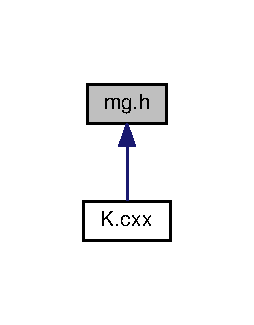
\includegraphics[width=122pt]{mg_8h__dep__incl}
\end{center}
\end{figure}
\subsection*{Data Structures}
\begin{DoxyCompactItemize}
\item 
class \hyperlink{class_k_1_1_m_g}{MG}
\end{DoxyCompactItemize}
\subsection*{Namespaces}
\begin{DoxyCompactItemize}
\item 
 \hyperlink{namespace_k}{K}
\end{DoxyCompactItemize}

\hypertarget{og_8h}{}\section{og.\+h File Reference}
\label{og_8h}\index{og.\+h@{og.\+h}}
This graph shows which files directly or indirectly include this file\+:
\nopagebreak
\begin{figure}[H]
\begin{center}
\leavevmode
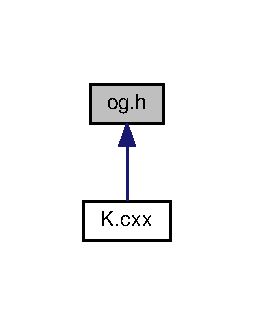
\includegraphics[width=122pt]{og_8h__dep__incl}
\end{center}
\end{figure}
\subsection*{Data Structures}
\begin{DoxyCompactItemize}
\item 
class \hyperlink{class_k_1_1_o_g}{OG}
\end{DoxyCompactItemize}
\subsection*{Namespaces}
\begin{DoxyCompactItemize}
\item 
 \hyperlink{namespace_k}{K}
\end{DoxyCompactItemize}

\hypertarget{pg_8h}{}\section{pg.\+h File Reference}
\label{pg_8h}\index{pg.\+h@{pg.\+h}}
This graph shows which files directly or indirectly include this file\+:
\nopagebreak
\begin{figure}[H]
\begin{center}
\leavevmode
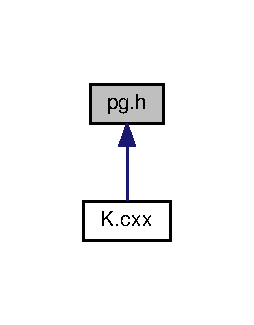
\includegraphics[width=122pt]{pg_8h__dep__incl}
\end{center}
\end{figure}
\subsection*{Data Structures}
\begin{DoxyCompactItemize}
\item 
class \hyperlink{class_k_1_1_p_g}{PG}
\end{DoxyCompactItemize}
\subsection*{Namespaces}
\begin{DoxyCompactItemize}
\item 
 \hyperlink{namespace_k}{K}
\end{DoxyCompactItemize}
\subsection*{Macros}
\begin{DoxyCompactItemize}
\item 
\#define \hyperlink{pg_8h_a958e4508ed28ee5cc04249144312c15f}{M\+\_\+\+P\+I\+\_\+2}~1.\+5707963267948965579989817342720925807952880859375
\end{DoxyCompactItemize}


\subsection{Macro Definition Documentation}
\index{pg.\+h@{pg.\+h}!M\+\_\+\+P\+I\+\_\+2@{M\+\_\+\+P\+I\+\_\+2}}
\index{M\+\_\+\+P\+I\+\_\+2@{M\+\_\+\+P\+I\+\_\+2}!pg.\+h@{pg.\+h}}
\subsubsection[{\texorpdfstring{M\+\_\+\+P\+I\+\_\+2}{M_PI_2}}]{\setlength{\rightskip}{0pt plus 5cm}\#define M\+\_\+\+P\+I\+\_\+2~1.\+5707963267948965579989817342720925807952880859375}\hypertarget{pg_8h_a958e4508ed28ee5cc04249144312c15f}{}\label{pg_8h_a958e4508ed28ee5cc04249144312c15f}


Definition at line 5 of file pg.\+h.


\hypertarget{qe_8h}{}\section{qe.\+h File Reference}
\label{qe_8h}\index{qe.\+h@{qe.\+h}}
This graph shows which files directly or indirectly include this file\+:
\nopagebreak
\begin{figure}[H]
\begin{center}
\leavevmode
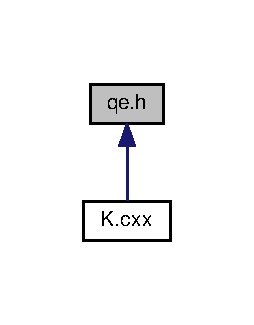
\includegraphics[width=122pt]{qe_8h__dep__incl}
\end{center}
\end{figure}
\subsection*{Data Structures}
\begin{DoxyCompactItemize}
\item 
class \hyperlink{class_k_1_1_q_e}{QE}
\end{DoxyCompactItemize}
\subsection*{Namespaces}
\begin{DoxyCompactItemize}
\item 
 \hyperlink{namespace_k}{K}
\end{DoxyCompactItemize}

\hypertarget{qp_8h}{}\section{qp.\+h File Reference}
\label{qp_8h}\index{qp.\+h@{qp.\+h}}
This graph shows which files directly or indirectly include this file\+:
\nopagebreak
\begin{figure}[H]
\begin{center}
\leavevmode
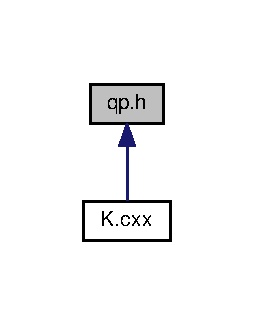
\includegraphics[width=122pt]{qp_8h__dep__incl}
\end{center}
\end{figure}
\subsection*{Data Structures}
\begin{DoxyCompactItemize}
\item 
class \hyperlink{class_k_1_1_q_p}{QP}
\end{DoxyCompactItemize}
\subsection*{Namespaces}
\begin{DoxyCompactItemize}
\item 
 \hyperlink{namespace_k}{K}
\end{DoxyCompactItemize}

\hypertarget{sh_8h}{}\section{sh.\+h File Reference}
\label{sh_8h}\index{sh.\+h@{sh.\+h}}
This graph shows which files directly or indirectly include this file\+:
\nopagebreak
\begin{figure}[H]
\begin{center}
\leavevmode
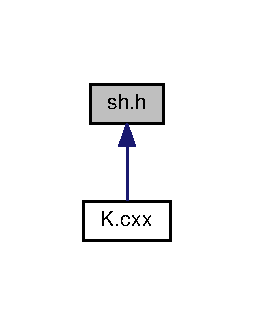
\includegraphics[width=122pt]{sh_8h__dep__incl}
\end{center}
\end{figure}
\subsection*{Data Structures}
\begin{DoxyCompactItemize}
\item 
class \hyperlink{class_k_1_1_s_h}{SH}
\end{DoxyCompactItemize}
\subsection*{Namespaces}
\begin{DoxyCompactItemize}
\item 
 \hyperlink{namespace_k}{K}
\end{DoxyCompactItemize}
\subsection*{Macros}
\begin{DoxyCompactItemize}
\item 
\#define \hyperlink{sh_8h_a7a276367773516f9f6e660c3f4635beb}{\+\_\+red\+Alert\+\_\+}~((SH$\ast$)screen)-\/$>$error
\end{DoxyCompactItemize}
\subsection*{Variables}
\begin{DoxyCompactItemize}
\item 
vector$<$ function$<$ void()$>$ $\ast$ $>$ \hyperlink{namespace_k_a1c3ecbe3046298af183be61349de6900}{ending\+Fn}
\item 
char \hyperlink{namespace_k_a1203c8bea34ade1c1d524b0df5bfdf37}{R\+B\+L\+A\+CK} \mbox{[}$\,$\mbox{]} = \char`\"{}\textbackslash{}033\mbox{[}0;30m\char`\"{}
\item 
char \hyperlink{namespace_k_ae976a2e4e900318926db4fa1624bc30a}{R\+R\+ED} \mbox{[}$\,$\mbox{]} = \char`\"{}\textbackslash{}033\mbox{[}0;31m\char`\"{}
\item 
char \hyperlink{namespace_k_a9c4858b8b93beb509648e92071d727ca}{R\+G\+R\+E\+EN} \mbox{[}$\,$\mbox{]} = \char`\"{}\textbackslash{}033\mbox{[}0;32m\char`\"{}
\item 
char \hyperlink{namespace_k_abd378d9900fa5f1effc177ef1a3eaf88}{R\+Y\+E\+L\+L\+OW} \mbox{[}$\,$\mbox{]} = \char`\"{}\textbackslash{}033\mbox{[}0;33m\char`\"{}
\item 
char \hyperlink{namespace_k_a035ca76c4d8abd4253d53e1dfb952368}{R\+B\+L\+UE} \mbox{[}$\,$\mbox{]} = \char`\"{}\textbackslash{}033\mbox{[}0;34m\char`\"{}
\item 
char \hyperlink{namespace_k_a16f016905667739f3d64b6ab7e4d7f95}{R\+P\+U\+R\+P\+LE} \mbox{[}$\,$\mbox{]} = \char`\"{}\textbackslash{}033\mbox{[}0;35m\char`\"{}
\item 
char \hyperlink{namespace_k_a816b9af371d1741fead9f73abb978052}{R\+C\+Y\+AN} \mbox{[}$\,$\mbox{]} = \char`\"{}\textbackslash{}033\mbox{[}0;36m\char`\"{}
\item 
char \hyperlink{namespace_k_a37a06065638319240adf83b5bdfdf313}{R\+W\+H\+I\+TE} \mbox{[}$\,$\mbox{]} = \char`\"{}\textbackslash{}033\mbox{[}0;37m\char`\"{}
\item 
char \hyperlink{namespace_k_a1b5ebfb775cf88920f1beb1b59c80137}{B\+B\+L\+A\+CK} \mbox{[}$\,$\mbox{]} = \char`\"{}\textbackslash{}033\mbox{[}1;30m\char`\"{}
\item 
char \hyperlink{namespace_k_ae09107156acfd00c2e31f049f70b622a}{B\+R\+ED} \mbox{[}$\,$\mbox{]} = \char`\"{}\textbackslash{}033\mbox{[}1;31m\char`\"{}
\item 
char \hyperlink{namespace_k_aa83d8d71c463813bdbd57fab20312b7d}{B\+G\+R\+E\+EN} \mbox{[}$\,$\mbox{]} = \char`\"{}\textbackslash{}033\mbox{[}1;32m\char`\"{}
\item 
char \hyperlink{namespace_k_aa522b04bcf50df65fd4819d0b46d6664}{B\+Y\+E\+L\+L\+OW} \mbox{[}$\,$\mbox{]} = \char`\"{}\textbackslash{}033\mbox{[}1;33m\char`\"{}
\item 
char \hyperlink{namespace_k_a2fcd49453f10ffd3ccb5aebe30f5d0c0}{B\+B\+L\+UE} \mbox{[}$\,$\mbox{]} = \char`\"{}\textbackslash{}033\mbox{[}1;34m\char`\"{}
\item 
char \hyperlink{namespace_k_adcaba86455bd5bd0cbdeac28c4fced2b}{B\+P\+U\+R\+P\+LE} \mbox{[}$\,$\mbox{]} = \char`\"{}\textbackslash{}033\mbox{[}1;35m\char`\"{}
\item 
char \hyperlink{namespace_k_a2c3e50cb34db635087047ef75ab1ca52}{B\+C\+Y\+AN} \mbox{[}$\,$\mbox{]} = \char`\"{}\textbackslash{}033\mbox{[}1;36m\char`\"{}
\item 
char \hyperlink{namespace_k_a723a80b3fad44765a8c6371fd4841609}{B\+W\+H\+I\+TE} \mbox{[}$\,$\mbox{]} = \char`\"{}\textbackslash{}033\mbox{[}1;37m\char`\"{}
\item 
char \hyperlink{namespace_k_a610d2184e75b6475eaf1f16700be824e}{R\+R\+E\+S\+ET} \mbox{[}$\,$\mbox{]} = \char`\"{}\textbackslash{}033\mbox{[}0m\char`\"{}
\end{DoxyCompactItemize}


\subsection{Macro Definition Documentation}
\index{sh.\+h@{sh.\+h}!\+\_\+red\+Alert\+\_\+@{\+\_\+red\+Alert\+\_\+}}
\index{\+\_\+red\+Alert\+\_\+@{\+\_\+red\+Alert\+\_\+}!sh.\+h@{sh.\+h}}
\subsubsection[{\texorpdfstring{\+\_\+red\+Alert\+\_\+}{_redAlert_}}]{\setlength{\rightskip}{0pt plus 5cm}\#define \+\_\+red\+Alert\+\_\+~((SH$\ast$)screen)-\/$>$error}\hypertarget{sh_8h_a7a276367773516f9f6e660c3f4635beb}{}\label{sh_8h_a7a276367773516f9f6e660c3f4635beb}


Definition at line 4 of file sh.\+h.


\hypertarget{ui_8h}{}\section{ui.\+h File Reference}
\label{ui_8h}\index{ui.\+h@{ui.\+h}}
This graph shows which files directly or indirectly include this file\+:
\nopagebreak
\begin{figure}[H]
\begin{center}
\leavevmode
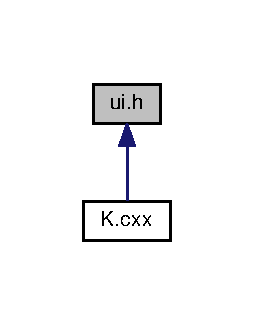
\includegraphics[width=122pt]{ui_8h__dep__incl}
\end{center}
\end{figure}
\subsection*{Data Structures}
\begin{DoxyCompactItemize}
\item 
class \hyperlink{class_k_1_1_u_i}{UI}
\end{DoxyCompactItemize}
\subsection*{Namespaces}
\begin{DoxyCompactItemize}
\item 
 \hyperlink{namespace_k}{K}
\end{DoxyCompactItemize}
\subsection*{Variables}
\begin{DoxyCompactItemize}
\item 
const char \hyperlink{ui_8h_a0568773bbf1975eb30c34fd8dc066549}{\+\_\+www\+\_\+html\+\_\+index}
\item 
const char \hyperlink{ui_8h_a26b0b9043782b3b1cc00326c741f836b}{\+\_\+www\+\_\+ico\+\_\+favicon}
\item 
const char \hyperlink{ui_8h_a6ab05f623b0e5c08a170e5334bfc1ba0}{\+\_\+www\+\_\+css\+\_\+base}
\item 
const char \hyperlink{ui_8h_aa2945a301b33dccaa4279adf2eae3cd4}{\+\_\+www\+\_\+gzip\+\_\+bomb}
\item 
const char \hyperlink{ui_8h_a4251341dfc79da09dc340e062cbb47f9}{\+\_\+www\+\_\+mp3\+\_\+audio\+\_\+0}
\item 
const char \hyperlink{ui_8h_a27e6829febcdeda2854a5285440d8f11}{\+\_\+www\+\_\+css\+\_\+light}
\item 
const char \hyperlink{ui_8h_aacf7df2eda9f5f86d358c33eeb5a4adb}{\+\_\+www\+\_\+js\+\_\+bundle}
\item 
const char \hyperlink{ui_8h_ab9086766055cf92ed18a17162b1be411}{\+\_\+www\+\_\+mp3\+\_\+audio\+\_\+1}
\item 
const char \hyperlink{ui_8h_a54ca4b3ec51bb57443eb988dc3367f3e}{\+\_\+www\+\_\+css\+\_\+dark}
\item 
const int \hyperlink{ui_8h_ae1bb0d3e9fd909bd48a2987eb115b287}{\+\_\+www\+\_\+html\+\_\+index\+\_\+len}
\item 
const int \hyperlink{ui_8h_a5957a5a67fc3dbc583929f7659dc7937}{\+\_\+www\+\_\+ico\+\_\+favicon\+\_\+len}
\item 
const int \hyperlink{ui_8h_a7c16f9081fa72b59304b449f30d0c059}{\+\_\+www\+\_\+css\+\_\+base\+\_\+len}
\item 
const int \hyperlink{ui_8h_a686c0254b2ec3f4ad6e6af93efc154cc}{\+\_\+www\+\_\+gzip\+\_\+bomb\+\_\+len}
\item 
const int \hyperlink{ui_8h_a43f1c4d8866c96e27564eebc8f75a2da}{\+\_\+www\+\_\+mp3\+\_\+audio\+\_\+0\+\_\+len}
\item 
const int \hyperlink{ui_8h_aef72cd4366d22e5b51a661288adbb2d2}{\+\_\+www\+\_\+css\+\_\+light\+\_\+len}
\item 
const int \hyperlink{ui_8h_a6be2966ac4e53987cf9fb997eb042ddb}{\+\_\+www\+\_\+js\+\_\+bundle\+\_\+len}
\item 
const int \hyperlink{ui_8h_ad631e51c75a7cab3f0b42edadcbde4f0}{\+\_\+www\+\_\+mp3\+\_\+audio\+\_\+1\+\_\+len}
\item 
const int \hyperlink{ui_8h_a670b5d2a617b2c4ffc6bc55ab6623930}{\+\_\+www\+\_\+css\+\_\+dark\+\_\+len}
\end{DoxyCompactItemize}


\subsection{Variable Documentation}
\index{ui.\+h@{ui.\+h}!\+\_\+www\+\_\+css\+\_\+base@{\+\_\+www\+\_\+css\+\_\+base}}
\index{\+\_\+www\+\_\+css\+\_\+base@{\+\_\+www\+\_\+css\+\_\+base}!ui.\+h@{ui.\+h}}
\subsubsection[{\texorpdfstring{\+\_\+www\+\_\+css\+\_\+base}{_www_css_base}}]{\setlength{\rightskip}{0pt plus 5cm}const char \+\_\+www\+\_\+css\+\_\+base}\hypertarget{ui_8h_a6ab05f623b0e5c08a170e5334bfc1ba0}{}\label{ui_8h_a6ab05f623b0e5c08a170e5334bfc1ba0}
\index{ui.\+h@{ui.\+h}!\+\_\+www\+\_\+css\+\_\+base\+\_\+len@{\+\_\+www\+\_\+css\+\_\+base\+\_\+len}}
\index{\+\_\+www\+\_\+css\+\_\+base\+\_\+len@{\+\_\+www\+\_\+css\+\_\+base\+\_\+len}!ui.\+h@{ui.\+h}}
\subsubsection[{\texorpdfstring{\+\_\+www\+\_\+css\+\_\+base\+\_\+len}{_www_css_base_len}}]{\setlength{\rightskip}{0pt plus 5cm}const int \+\_\+www\+\_\+css\+\_\+base\+\_\+len}\hypertarget{ui_8h_a7c16f9081fa72b59304b449f30d0c059}{}\label{ui_8h_a7c16f9081fa72b59304b449f30d0c059}
\index{ui.\+h@{ui.\+h}!\+\_\+www\+\_\+css\+\_\+dark@{\+\_\+www\+\_\+css\+\_\+dark}}
\index{\+\_\+www\+\_\+css\+\_\+dark@{\+\_\+www\+\_\+css\+\_\+dark}!ui.\+h@{ui.\+h}}
\subsubsection[{\texorpdfstring{\+\_\+www\+\_\+css\+\_\+dark}{_www_css_dark}}]{\setlength{\rightskip}{0pt plus 5cm}const char \+\_\+www\+\_\+css\+\_\+dark}\hypertarget{ui_8h_a54ca4b3ec51bb57443eb988dc3367f3e}{}\label{ui_8h_a54ca4b3ec51bb57443eb988dc3367f3e}
\index{ui.\+h@{ui.\+h}!\+\_\+www\+\_\+css\+\_\+dark\+\_\+len@{\+\_\+www\+\_\+css\+\_\+dark\+\_\+len}}
\index{\+\_\+www\+\_\+css\+\_\+dark\+\_\+len@{\+\_\+www\+\_\+css\+\_\+dark\+\_\+len}!ui.\+h@{ui.\+h}}
\subsubsection[{\texorpdfstring{\+\_\+www\+\_\+css\+\_\+dark\+\_\+len}{_www_css_dark_len}}]{\setlength{\rightskip}{0pt plus 5cm}const int \+\_\+www\+\_\+css\+\_\+dark\+\_\+len}\hypertarget{ui_8h_a670b5d2a617b2c4ffc6bc55ab6623930}{}\label{ui_8h_a670b5d2a617b2c4ffc6bc55ab6623930}
\index{ui.\+h@{ui.\+h}!\+\_\+www\+\_\+css\+\_\+light@{\+\_\+www\+\_\+css\+\_\+light}}
\index{\+\_\+www\+\_\+css\+\_\+light@{\+\_\+www\+\_\+css\+\_\+light}!ui.\+h@{ui.\+h}}
\subsubsection[{\texorpdfstring{\+\_\+www\+\_\+css\+\_\+light}{_www_css_light}}]{\setlength{\rightskip}{0pt plus 5cm}const char \+\_\+www\+\_\+css\+\_\+light}\hypertarget{ui_8h_a27e6829febcdeda2854a5285440d8f11}{}\label{ui_8h_a27e6829febcdeda2854a5285440d8f11}
\index{ui.\+h@{ui.\+h}!\+\_\+www\+\_\+css\+\_\+light\+\_\+len@{\+\_\+www\+\_\+css\+\_\+light\+\_\+len}}
\index{\+\_\+www\+\_\+css\+\_\+light\+\_\+len@{\+\_\+www\+\_\+css\+\_\+light\+\_\+len}!ui.\+h@{ui.\+h}}
\subsubsection[{\texorpdfstring{\+\_\+www\+\_\+css\+\_\+light\+\_\+len}{_www_css_light_len}}]{\setlength{\rightskip}{0pt plus 5cm}const int \+\_\+www\+\_\+css\+\_\+light\+\_\+len}\hypertarget{ui_8h_aef72cd4366d22e5b51a661288adbb2d2}{}\label{ui_8h_aef72cd4366d22e5b51a661288adbb2d2}
\index{ui.\+h@{ui.\+h}!\+\_\+www\+\_\+gzip\+\_\+bomb@{\+\_\+www\+\_\+gzip\+\_\+bomb}}
\index{\+\_\+www\+\_\+gzip\+\_\+bomb@{\+\_\+www\+\_\+gzip\+\_\+bomb}!ui.\+h@{ui.\+h}}
\subsubsection[{\texorpdfstring{\+\_\+www\+\_\+gzip\+\_\+bomb}{_www_gzip_bomb}}]{\setlength{\rightskip}{0pt plus 5cm}const char \+\_\+www\+\_\+gzip\+\_\+bomb}\hypertarget{ui_8h_aa2945a301b33dccaa4279adf2eae3cd4}{}\label{ui_8h_aa2945a301b33dccaa4279adf2eae3cd4}
\index{ui.\+h@{ui.\+h}!\+\_\+www\+\_\+gzip\+\_\+bomb\+\_\+len@{\+\_\+www\+\_\+gzip\+\_\+bomb\+\_\+len}}
\index{\+\_\+www\+\_\+gzip\+\_\+bomb\+\_\+len@{\+\_\+www\+\_\+gzip\+\_\+bomb\+\_\+len}!ui.\+h@{ui.\+h}}
\subsubsection[{\texorpdfstring{\+\_\+www\+\_\+gzip\+\_\+bomb\+\_\+len}{_www_gzip_bomb_len}}]{\setlength{\rightskip}{0pt plus 5cm}const int \+\_\+www\+\_\+gzip\+\_\+bomb\+\_\+len}\hypertarget{ui_8h_a686c0254b2ec3f4ad6e6af93efc154cc}{}\label{ui_8h_a686c0254b2ec3f4ad6e6af93efc154cc}
\index{ui.\+h@{ui.\+h}!\+\_\+www\+\_\+html\+\_\+index@{\+\_\+www\+\_\+html\+\_\+index}}
\index{\+\_\+www\+\_\+html\+\_\+index@{\+\_\+www\+\_\+html\+\_\+index}!ui.\+h@{ui.\+h}}
\subsubsection[{\texorpdfstring{\+\_\+www\+\_\+html\+\_\+index}{_www_html_index}}]{\setlength{\rightskip}{0pt plus 5cm}const char \+\_\+www\+\_\+html\+\_\+index}\hypertarget{ui_8h_a0568773bbf1975eb30c34fd8dc066549}{}\label{ui_8h_a0568773bbf1975eb30c34fd8dc066549}
\index{ui.\+h@{ui.\+h}!\+\_\+www\+\_\+html\+\_\+index\+\_\+len@{\+\_\+www\+\_\+html\+\_\+index\+\_\+len}}
\index{\+\_\+www\+\_\+html\+\_\+index\+\_\+len@{\+\_\+www\+\_\+html\+\_\+index\+\_\+len}!ui.\+h@{ui.\+h}}
\subsubsection[{\texorpdfstring{\+\_\+www\+\_\+html\+\_\+index\+\_\+len}{_www_html_index_len}}]{\setlength{\rightskip}{0pt plus 5cm}const int \+\_\+www\+\_\+html\+\_\+index\+\_\+len}\hypertarget{ui_8h_ae1bb0d3e9fd909bd48a2987eb115b287}{}\label{ui_8h_ae1bb0d3e9fd909bd48a2987eb115b287}
\index{ui.\+h@{ui.\+h}!\+\_\+www\+\_\+ico\+\_\+favicon@{\+\_\+www\+\_\+ico\+\_\+favicon}}
\index{\+\_\+www\+\_\+ico\+\_\+favicon@{\+\_\+www\+\_\+ico\+\_\+favicon}!ui.\+h@{ui.\+h}}
\subsubsection[{\texorpdfstring{\+\_\+www\+\_\+ico\+\_\+favicon}{_www_ico_favicon}}]{\setlength{\rightskip}{0pt plus 5cm}const char \+\_\+www\+\_\+ico\+\_\+favicon}\hypertarget{ui_8h_a26b0b9043782b3b1cc00326c741f836b}{}\label{ui_8h_a26b0b9043782b3b1cc00326c741f836b}
\index{ui.\+h@{ui.\+h}!\+\_\+www\+\_\+ico\+\_\+favicon\+\_\+len@{\+\_\+www\+\_\+ico\+\_\+favicon\+\_\+len}}
\index{\+\_\+www\+\_\+ico\+\_\+favicon\+\_\+len@{\+\_\+www\+\_\+ico\+\_\+favicon\+\_\+len}!ui.\+h@{ui.\+h}}
\subsubsection[{\texorpdfstring{\+\_\+www\+\_\+ico\+\_\+favicon\+\_\+len}{_www_ico_favicon_len}}]{\setlength{\rightskip}{0pt plus 5cm}const int \+\_\+www\+\_\+ico\+\_\+favicon\+\_\+len}\hypertarget{ui_8h_a5957a5a67fc3dbc583929f7659dc7937}{}\label{ui_8h_a5957a5a67fc3dbc583929f7659dc7937}
\index{ui.\+h@{ui.\+h}!\+\_\+www\+\_\+js\+\_\+bundle@{\+\_\+www\+\_\+js\+\_\+bundle}}
\index{\+\_\+www\+\_\+js\+\_\+bundle@{\+\_\+www\+\_\+js\+\_\+bundle}!ui.\+h@{ui.\+h}}
\subsubsection[{\texorpdfstring{\+\_\+www\+\_\+js\+\_\+bundle}{_www_js_bundle}}]{\setlength{\rightskip}{0pt plus 5cm}const char \+\_\+www\+\_\+js\+\_\+bundle}\hypertarget{ui_8h_aacf7df2eda9f5f86d358c33eeb5a4adb}{}\label{ui_8h_aacf7df2eda9f5f86d358c33eeb5a4adb}
\index{ui.\+h@{ui.\+h}!\+\_\+www\+\_\+js\+\_\+bundle\+\_\+len@{\+\_\+www\+\_\+js\+\_\+bundle\+\_\+len}}
\index{\+\_\+www\+\_\+js\+\_\+bundle\+\_\+len@{\+\_\+www\+\_\+js\+\_\+bundle\+\_\+len}!ui.\+h@{ui.\+h}}
\subsubsection[{\texorpdfstring{\+\_\+www\+\_\+js\+\_\+bundle\+\_\+len}{_www_js_bundle_len}}]{\setlength{\rightskip}{0pt plus 5cm}const int \+\_\+www\+\_\+js\+\_\+bundle\+\_\+len}\hypertarget{ui_8h_a6be2966ac4e53987cf9fb997eb042ddb}{}\label{ui_8h_a6be2966ac4e53987cf9fb997eb042ddb}
\index{ui.\+h@{ui.\+h}!\+\_\+www\+\_\+mp3\+\_\+audio\+\_\+0@{\+\_\+www\+\_\+mp3\+\_\+audio\+\_\+0}}
\index{\+\_\+www\+\_\+mp3\+\_\+audio\+\_\+0@{\+\_\+www\+\_\+mp3\+\_\+audio\+\_\+0}!ui.\+h@{ui.\+h}}
\subsubsection[{\texorpdfstring{\+\_\+www\+\_\+mp3\+\_\+audio\+\_\+0}{_www_mp3_audio_0}}]{\setlength{\rightskip}{0pt plus 5cm}const char \+\_\+www\+\_\+mp3\+\_\+audio\+\_\+0}\hypertarget{ui_8h_a4251341dfc79da09dc340e062cbb47f9}{}\label{ui_8h_a4251341dfc79da09dc340e062cbb47f9}
\index{ui.\+h@{ui.\+h}!\+\_\+www\+\_\+mp3\+\_\+audio\+\_\+0\+\_\+len@{\+\_\+www\+\_\+mp3\+\_\+audio\+\_\+0\+\_\+len}}
\index{\+\_\+www\+\_\+mp3\+\_\+audio\+\_\+0\+\_\+len@{\+\_\+www\+\_\+mp3\+\_\+audio\+\_\+0\+\_\+len}!ui.\+h@{ui.\+h}}
\subsubsection[{\texorpdfstring{\+\_\+www\+\_\+mp3\+\_\+audio\+\_\+0\+\_\+len}{_www_mp3_audio_0_len}}]{\setlength{\rightskip}{0pt plus 5cm}const int \+\_\+www\+\_\+mp3\+\_\+audio\+\_\+0\+\_\+len}\hypertarget{ui_8h_a43f1c4d8866c96e27564eebc8f75a2da}{}\label{ui_8h_a43f1c4d8866c96e27564eebc8f75a2da}
\index{ui.\+h@{ui.\+h}!\+\_\+www\+\_\+mp3\+\_\+audio\+\_\+1@{\+\_\+www\+\_\+mp3\+\_\+audio\+\_\+1}}
\index{\+\_\+www\+\_\+mp3\+\_\+audio\+\_\+1@{\+\_\+www\+\_\+mp3\+\_\+audio\+\_\+1}!ui.\+h@{ui.\+h}}
\subsubsection[{\texorpdfstring{\+\_\+www\+\_\+mp3\+\_\+audio\+\_\+1}{_www_mp3_audio_1}}]{\setlength{\rightskip}{0pt plus 5cm}const char \+\_\+www\+\_\+mp3\+\_\+audio\+\_\+1}\hypertarget{ui_8h_ab9086766055cf92ed18a17162b1be411}{}\label{ui_8h_ab9086766055cf92ed18a17162b1be411}
\index{ui.\+h@{ui.\+h}!\+\_\+www\+\_\+mp3\+\_\+audio\+\_\+1\+\_\+len@{\+\_\+www\+\_\+mp3\+\_\+audio\+\_\+1\+\_\+len}}
\index{\+\_\+www\+\_\+mp3\+\_\+audio\+\_\+1\+\_\+len@{\+\_\+www\+\_\+mp3\+\_\+audio\+\_\+1\+\_\+len}!ui.\+h@{ui.\+h}}
\subsubsection[{\texorpdfstring{\+\_\+www\+\_\+mp3\+\_\+audio\+\_\+1\+\_\+len}{_www_mp3_audio_1_len}}]{\setlength{\rightskip}{0pt plus 5cm}const int \+\_\+www\+\_\+mp3\+\_\+audio\+\_\+1\+\_\+len}\hypertarget{ui_8h_ad631e51c75a7cab3f0b42edadcbde4f0}{}\label{ui_8h_ad631e51c75a7cab3f0b42edadcbde4f0}

%--- End generated contents ---

% Index
\backmatter
\newpage
\phantomsection
\clearemptydoublepage
\addcontentsline{toc}{chapter}{Index}
\printindex

\end{document}
